\documentclass[a4paper, 12pt]{article}
\usepackage{amsmath, amsfonts, amssymb}
\usepackage{array}
\usepackage{booktabs}
\usepackage[figurename=Figure]{caption}
\usepackage{float}
\usepackage[margin=2.3cm]{geometry}
\usepackage{graphicx}
\usepackage{hyperref}
\usepackage[utf8]{inputenc}
\usepackage{multirow}
\usepackage{setspace}
\usepackage{subcaption}
\usepackage{pdflscape}
\usepackage[round]{natbib}
\bibliographystyle{aer}

\hypersetup{
  colorlinks=false,
  linkcolor=black,
  filecolor=black,
  urlcolor=black,
  citecolor=black,
}

\setlength{\tabcolsep}{3pt}

\newcolumntype{L}[1]{>{\raggedright\let\newline\\\arraybackslash\hspace{0pt}}m{#1}}
\newcolumntype{C}[1]{>{\centering\let\newline\\\arraybackslash\hspace{0pt}}m{#1}}

\raggedbottom

%Prevent footnotes from splitting across pages
\interfootnotelinepenalty=10000

\begin{document}
\onehalfspacing

\begin{center}
{\LARGE Supplemental Appendix} \\[0.5cm]
{\large Survival versus Scale: The Effects of Critical Access Hospital Designation}
\end{center}

\vspace{1cm}

This appendix provides supplementary material for the main text. Section~\ref{sec:app-financial} details the construction of our hospital-level financial measures. Section~\ref{sec:app-diagnostics} reports diagnostics for the synthetic difference-in-differences (SDID) estimator, including sample attrition from balanced-panel requirements, pre-trend tests, and synthetic control weight concentration. Section~\ref{sec:app-sample} examines sensitivity to the estimation sample, including the control group construction, pre-period length, bed size cutoff, and the eligibility-restricted design. Section~\ref{sec:app-alt} presents results from alternative estimators (Callaway--Sant'Anna and interactive fixed effects). Section~\ref{sec:app-perm} reports permutation inference results. Section~\ref{sec:app-adoption} examines what predicts a state's adoption year, Section~\ref{sec:app-populations} compares converting hospitals with hospitals that closed and reports bed reductions by initial size, and Section~\ref{sec:app-anticipation} reports the eligibility-restricted version of the pre-designation restructuring analysis in the main text.


%%% ===================================================================
%%% SECTION 1: Financial Measure Construction
%%% ===================================================================

\section{Financial Measure Construction}
\label{sec:app-financial}

We construct six financial measures (operating margin, current ratio, net patient revenue per bed, total operating expenses per bed, net fixed assets per bed, and capital expenditures per bed) from the Healthcare Cost Report Information System (HCRIS). This section describes the crosswalk that links converting hospitals to their pre-designation cost reports, the measure definitions, and the post-processing steps.

\subsection{Data Sources}

\paragraph{\textit{HCRIS.}} Medicare-certified hospitals file annual cost reports, from which we extract net patient revenue, total operating expenses, current assets, current liabilities, net fixed assets (land, buildings, and equipment net of accumulated depreciation), and the components of accumulated depreciation. These fields are drawn from Worksheet G (balance sheet) and Worksheet G-3 (income statement) of the cost report. When a hospital files multiple non-overlapping reports in a single fiscal year, we sum the relevant fields across reports. CMS publishes cost report data beginning with fiscal year 1996, so our financial series begins in 1996.

\paragraph{\textit{Linking converters to their pre-designation cost reports.}} Cost reports are identified by Medicare provider number, and a hospital receives a new number when it is designated as a CAH. We therefore match each converter's pre-designation years to cost reports filed under non-CAH provider numbers in the same state, using name similarity within zip code or city. We drop earlier numbers claimed by two converters, numbers that belong to another hospital, and numbers whose reports continue for more than two years after designation. Of converters' pre-designation hospital-years from 1996 onward, 86 percent have a cost report, compared with 15 percent under a time-invariant crosswalk that assigns each hospital one provider number for all years.

\subsection{Measure Definitions}

\paragraph{\textit{Operating margin.}} Operating margin is defined as
$$
\text{margin} = \frac{\text{net patient revenue} - \text{total operating expenses}}{\text{net patient revenue}}.
$$

\paragraph{\textit{Current ratio.}} The current ratio is defined as
$$
\text{current ratio} = \frac{\text{current assets}}{\text{current liabilities}},
$$
where both fields are drawn from the balance sheet (Worksheet G).

\paragraph{\textit{Net fixed assets per bed.}} Net fixed assets are taken directly from the HCRIS balance sheet. We normalize by each hospital's pre-period mean bed count, computed as the average of total staffed beds (AHA variable \texttt{BDTOT}) across all years after 1995 and prior to CAH designation (or across all post-1995 years for hospitals that never receive designation). We deflate to constant 2010 dollars using the annual CPI-U and express the result in millions of dollars per bed:
$$
\text{net fixed assets per bed} = \frac{\text{net fixed assets}}{10^6 \times \bar{B}_{\text{pre}} \times \text{CPI deflator}},
$$
where $\bar{B}_{\text{pre}}$ is the pre-period mean bed count and the CPI deflator is the ratio of the current-year CPI-U index to the 2010 index.

\paragraph{\textit{Capital expenditures per bed.}} We approximate capital expenditures as the year-to-year change in gross fixed assets. Gross fixed assets are computed as net fixed assets plus accumulated depreciation; capital expenditure is then the first difference of this series within each hospital. As with net fixed assets, we normalize by the pre-period mean bed count and deflate to constant 2010 dollars, expressed in units of \$10,000 per bed:
$$
\text{capex per bed} = \frac{\Delta\text{gross fixed assets}}{10^4 \times \bar{B}_{\text{pre}} \times \text{CPI deflator}}.
$$

\paragraph{\textit{Net patient revenue per bed.}} Net patient revenue is taken from the HCRIS income statement. We normalize by each hospital's pre-period mean bed count and deflate to constant 2010 dollars using the CPI-U, expressed in thousands of dollars per bed:
$$
\text{net patient revenue per bed} = \frac{\text{net patient revenue}}{10^3 \times \bar{B}_{\text{pre}} \times \text{CPI deflator}}.
$$

\paragraph{\textit{Total operating expenses per bed.}} Total operating expenses are taken from the HCRIS income statement. As with revenue, we normalize by the pre-period mean bed count and deflate to constant 2010 dollars, expressed in thousands of dollars per bed:
$$
\text{operating expenses per bed} = \frac{\text{total operating expenses}}{10^3 \times \bar{B}_{\text{pre}} \times \text{CPI deflator}}.
$$

\noindent Because operating margin is defined as $(R - C)/R$, these two component measures allow us to assess whether changes in margins reflect movements in revenue, costs, or both. The revenue and expense measures are constructed after computing operating margin from raw values, so the winsorization and per-bed normalization applied to these components do not affect the margin calculation.

\subsection{Post-Processing}

\paragraph{\textit{Winsorization.}} We winsorize all six financial measures at the 5th and 95th percentiles within each year-by-ever-CAH cell. Winsorization is applied before CPI deflation and per-bed normalization of the capital and revenue/expense measures. This reduces the influence of extreme values driven by reporting anomalies while preserving cross-sectional and temporal variation within plausible ranges.

\paragraph{\textit{Interpolation.}} After winsorization, we linearly interpolate missing values within each hospital's time series using observed year as the time index. Interpolation fills isolated gaps (e.g., a single missing cost report year) while leaving leading and trailing missingness unchanged. The same winsorization and interpolation procedures are applied to the capacity and staffing variables (total beds, OB beds, and FTE RNs), and inpatient days per bed is interpolated in the same way after being capped at 85 percent occupancy.


%%% ===================================================================
%%% SECTION 2: SDID Diagnostics
%%% ===================================================================

\section{SDID Diagnostics}
\label{sec:app-diagnostics}

Our primary estimates use the synthetic difference-in-differences (SDID) estimator, which requires a balanced panel of units observed in every period of the event window \citep{arkhangelsky2021}. This requirement can reduce sample sizes relative to estimators that accommodate unbalanced panels, such as the Callaway and Sant'Anna (CS) estimator \citep{callaway2021}. Similarly, the SDID estimator assigns nonnegative weights to control units to match the treated group's pre-period trajectory. If these weights are highly concentrated on a small number of controls, the resulting estimates may be sensitive to idiosyncratic variation in those units. We present three diagnostics below to assess these concerns.

Table~\ref{tab:diag-sample} reports, for each outcome and cohort, the number of treated and control units in the SDID balanced panel and in the full sample before balancing, together with the share of units lost to balancing. Attrition is largest for system membership, where roughly two-thirds of units in every cohort drop out of the balanced panel, and for the 1999 cohort of the financial outcomes, whose event window reaches back to the first years of the cost report data. Table~\ref{tab:diag-weights} reports the number of control units, the largest weight on any single control, the share of weight on the five largest controls, and the Herfindahl index of the weights. For the hospital-level outcomes, the largest weight on any control is at most 0.06 and the five largest controls never carry more than 27 percent of the weight, so no estimate depends on a handful of controls. The state-level outcomes have far fewer controls, 5 to 21 states depending on the cohort, so their weights are necessarily more concentrated.

Whether converters and the control pool were on different paths before designation indicates how much the SDID weights have to correct and which outcomes show restructuring before designation. Table~\ref{tab:diag-pretrend} therefore reports pre-trend tests on the unweighted balanced panel, regressing each outcome on the interaction of event time and treatment status over pre-treatment observations. The fit of the synthetic control itself is visible in the treated and synthetic paths in the main-text figures.

The FTE RN outcome shows evidence of differential pre-trends in the 1999 and 2000 cohorts (Table~\ref{tab:diag-pretrend}). This is consistent with treated hospitals already reducing staffing before formal designation, reflecting the restructuring required to meet eligibility requirements, which the main text examines directly by dating treatment one year earlier.

Among the financial outcomes, operating margin and the current ratio show statistically significant differential pre-trends in the 2000 and 2001 cohorts, total operating expenses per bed in the 1999 cohort, and net fixed assets in the 2000 cohort, while net patient revenue per bed shows none. The margin and expense pre-trends are consistent with the same pre-designation restructuring, in which converters' margins decline in the two years before designation as they shed scale, a pattern the main text documents directly. As shown in Section~\ref{sec:app-sample}, SDID point estimates for the financial outcomes are stable across pre-period lengths of 2--5 years. Among the organizational outcomes, closures show marginal pre-trends of opposite sign in the 2000 and 2001 cohorts and mergers in 1999, none at the 5 percent level.


%%% ===================================================================
%%% SECTION 3: Sensitivity to Estimation Sample
%%% ===================================================================

\section{Sensitivity to Estimation Sample}
\label{sec:app-sample}

Our results may be sensitive to how the estimation sample is defined. In this section, we examine sensitivity along several dimensions: the required lag in state-level CAH adoption, the post-period event window length, the exclusion of immediate adopters, the exclusion of never-treated states, the bed size cutoff used to define sample eligibility, the pre-period length for financial outcomes, and the eligibility-restricted control group design.

\paragraph{\textit{State-level adoption lags.}}
Our main specification constructs the not-yet-treated control group by requiring that a state's first CAH designation occur strictly after the cohort year. Formally, for a treated cohort converting in year $t$, a not-yet-treated hospital enters the control pool only if its state's first CAH designation year satisfies $s > t + \delta$, where $\delta = 0$ in the baseline. Increasing $\delta$ strengthens the exclusion by removing states whose CAH programs begin shortly after the cohort year, reducing the risk that anticipation effects or early program spillovers contaminate the control group. The cost is a smaller control pool, which reduces precision and may alter the composition of comparison units.

Figure~\ref{fig:statecut-sensitivity} presents SDID estimates for all outcomes at $\delta = 1$ and $\delta = 2$ alongside the baseline ($\delta = 0$). We do not report $\delta = 3$ because the earliest cohort (1999) can only draw controls from states adopting in 2003 or later, leaving too few comparison units for reliable estimation. The shaded band in each panel spans the baseline 95\% confidence interval, and the dashed vertical line marks the baseline point estimate. Across all outcomes, the sensitivity estimates remain qualitatively similar to the baseline, showing capacity reductions, system membership increases, and positive margin effects at both lag values. Point estimates generally fall within or near the baseline confidence band, confirming that our findings are not driven by contamination from states that adopt CAH programs shortly after the cohort year.

\paragraph{\textit{Post-period event window.}}
Our baseline uses a 5-year post-period, meaning control hospitals must not convert to CAH within 5 years of the cohort year. This requirement mechanically excludes hospitals that convert soon after their state opens the CAH program, selecting late- or never-converters into the control pool. If these hospitals differ systematically from treated hospitals (e.g., in financial health, management capacity, or payer mix), the exclusion could bias the comparison. Shortening the post-period to 4, 3, or 2 years relaxes this restriction, allowing hospitals that took up CAH relatively quickly after state implementation to serve as controls. Figure~\ref{fig:postperiod-sensitivity} reports SDID estimates at post-period lengths of 5, 4, 3, and 2 years. The results are broadly stable across all post-period lengths, with capacity reductions, closure effects, and positive margin effects persisting even at the shortest 2-year window.

\paragraph{\textit{Excluding immediate adopters.}}
Hospitals that convert to CAH in the same year their state first implements the program may represent a selected group of particularly proactive or financially distressed facilities. To assess whether these ``immediate adopters'' drive our results, we re-estimate the main specification after reclassifying them as untreated. Of the 1,466 hospitals with a designation date anywhere in our panel, 121 (8.3\%) converted in their state's first year of CAH availability. Figure~\ref{fig:noimmediate-sensitivity} shows that dropping these hospitals has minimal effect on the estimates, with point estimates for all outcomes remaining close to the baseline.

\paragraph{\textit{Excluding never-treated states.}}
The control pool in our main specification includes hospitals from states that never adopted CAH designation during our sample period. These states (Connecticut, New Jersey, and Rhode Island) are relatively urban, raising the concern that their hospitals may not be comparable to treated hospitals in rural states. However, only 10 hospitals in these states have 50 or fewer beds in any year, so they contribute minimally to the control group after the bed size restriction. Figure~\ref{fig:nonever-sensitivity} confirms that excluding never-treated states entirely has negligible effects on the estimates.

\paragraph{\textit{Bed size cutoff.}}
We also examine sensitivity to the bed size cutoff used to define the sample of plausibly CAH-eligible hospitals. Our baseline restricts to hospitals with 50 or fewer beds, allowing for flexible enforcement of CAH eligibility criteria as well as a buffer for hospitals that downsize to qualify. Figure~\ref{fig:bedcut-sensitivity} reports SDID estimates using cutoffs of 25 and 75 beds. Tightening the cutoff to 25 beds restricts the sample to hospitals already at or below the statutory limit, while relaxing it to 75 beds includes larger hospitals that may be less comparable to CAH converters. State-level outcomes (closures and mergers) are excluded because they do not depend on the hospital-level bed size filter. Across all hospital-level outcomes, the estimates are broadly consistent with the baseline, confirming that the results are not artifacts of the particular bed size threshold.

\paragraph{\textit{Pre-period length for financial outcomes.}}
Our financial series begins in 1996, so the baseline specification uses a three-year pre-period for financial outcomes in order to give every cohort a full pre-period. A longer pre-period does not add years for the earliest cohorts, because the balanced panel is formed only over the years with data, but it does change which hospitals enter the panel. With a five-year pre-period, for example, the treated sample falls from 272 to 143 hospitals. To assess sensitivity to this choice, we re-estimate each financial outcome using pre-periods of 2, 3, 4, and 5 years.

Table~\ref{tab:preperiod-financial} reports the results. Operating margin estimates range from 0.033 to 0.040 across pre-period lengths and are statistically significant at each. Net fixed assets per bed is close to zero throughout, and capital expenditures per bed is positive but imprecise. Current ratio estimates range from $-0.371$ (pre-period~$=5$) to $-0.206$ (pre-period~$=2$), and are significant only at the longest pre-period.

Net patient revenue per bed ranges from $-9.5$ to $-20.7$ thousand 2010 dollars per bed across pre-period lengths and operating expenses per bed from $-17.8$ to $-21.6$, with expenses falling by at least as much as revenue at every pre-period length. The stability of the point estimates across pre-period lengths, and across the treated samples they imply, indicates that the results are not driven by a particular subset of hospitals that happen to have unusually long financial histories.

\paragraph{\textit{Eligibility-restricted control group.}}
Table~\ref{tab:elig-overall} reports overall ATT estimates from the eligibility-restricted design, which uses all non-CAH or not-yet-CAH hospitals with $\leq 50$ beds as controls regardless of state-level CAH adoption timing. This design expands the cohort range to 1999--2005 and substantially increases treated sample sizes relative to the state-timing design. Closures and mergers are omitted because these outcomes are estimated at the state level and require the state-timing design.


%%% ===================================================================
%%% SECTION 4: Alternative Estimators
%%% ===================================================================

\section{Alternative Estimators}
\label{sec:app-alt}

\subsection{Callaway--Sant'Anna Event-Study Estimates}

This section presents Callaway and Sant'Anna (CS) event-study estimates. Event studies based on the state-timing design are presented in Figures~\ref{fig:cs-financial}--\ref{fig:cs-visits}, which underlie the overall CS ATTs presented in the main text. Analogous event-study estimates for the eligibility-restricted design are presented in Figures~\ref{fig:elig-cs-financial}--\ref{fig:elig-cs-visits}, along with the overall ATTs in Tables~\ref{tab:elig-overall} and~\ref{tab:visits-cs}.

\subsection{Interactive Fixed Effects Estimates}

Our primary SDID estimates require balanced panels, which can substantially reduce sample sizes, particularly for financial outcomes with sparse pre-treatment data coverage. As a robustness check, we estimate treatment effects using the interactive fixed effects (IFE) counterfactual estimator \citep{xu2017}, implemented in the \texttt{fect} package. The IFE estimator models untreated potential outcomes as a function of unit and time fixed effects plus a low-rank factor structure, then imputes counterfactual outcomes for treated observations. This approach accommodates unbalanced panels, so we retain the full sample of hospitals with available data.

We apply the IFE estimator to all financial and operational outcomes using the eligibility-restricted control group construction and a five-year pre-period. The operational outcomes use cohorts 1999--2005. The financial outcomes use cohorts 2001--2005, because the estimator requires at least five pre-treatment years and our financial series begins in 1996. For each cohort, we select the number of factors (0--5) by leave-one-out cross-validation and compute bootstrap standard errors (150 replications). Cohort-level ATTs are aggregated using the same treated-count weighting as our SDID estimates.

The IFE estimates are broadly consistent with the main SDID findings (Table~\ref{tab:gsynth}). Beds, OB beds, and FTE RNs decline by comparable magnitudes, and operating margin rises by 0.026 (95\% CI $[0.02, 0.03]$). Operating expenses per bed decline as under SDID, but net patient revenue per bed rises under IFE, so the revenue side of the decomposition is less stable across estimators than the margin itself. The current ratio, net fixed assets, and capital expenditures are close to zero. Ultimately, these estimates suggest that the main SDID results for capacity and margins do not depend on the balanced-panel restriction, nor do they appear to reflect differential trends that a latent factor structure would absorb.

%%% ===================================================================
%%% SECTION 5: Permutation Inference
%%% ===================================================================

\section{Permutation Inference}
\label{sec:app-perm}

The SDID estimator computes standard errors via the jackknife, which may perform poorly with small numbers of treated units. As a nonparametric alternative, we implement a permutation test. For each outcome, we randomly reassign treatment status among units within each cohort's balanced panel, holding the number of treated units fixed, and re-estimate the SDID ATT. We repeat this procedure 500 times to construct a placebo distribution. The permutation $p$-value is the fraction of placebo ATTs at least as extreme in absolute value as the actual estimate.

Figure~\ref{fig:permutation} displays the placebo distributions for all outcomes, and the main text reports the permutation $p$-values alongside the jackknife intervals. The permutation $p$-values are consistent with the jackknife-based confidence intervals. Total beds, OB beds, FTE RNs, operating margin, operating expenses per bed, and closures reject the null at conventional levels under both, while the current ratio, net fixed assets, capital expenditures, inpatient days per bed, and mergers do not under either. Net patient revenue per bed and system membership are significant under the jackknife but not under permutation ($p = 0.07$ and $0.09$). This alignment suggests that the jackknife standard errors provide a reasonable basis for inference despite the small number of treated units.


%%% ===================================================================
%%% SECTION: State Adoption Timing
%%% ===================================================================

\section{State Adoption Timing}
\label{sec:app-adoption}

To see whether observable characteristics predict a state's adoption cohort, we relate it to the state's hospital market structure, closure rates, operating margins, and unemployment rate over 1990 to 1996. Simple means and correlations are summarized in Table~\ref{tab:adoption-timing}. Across the 35 states in our 1999 to 2001 cohorts, earlier adopters are more rural and have more small hospitals. Specifically, the 1999 cohort is 37 percent rural against 23 percent for 2000 and 17 percent for 2001, and the correlation between cohort year and the number of hospitals with 50 or fewer beds is $-0.45$. Pre-period operating margins are about 2.5 points lower in the 1999 cohort than in the 2001 cohort.

In a simple regression of designation timing on rural share, the number of small hospitals, closure rates, and unemployment, rural share and the number of small hospitals are the only variables near conventional significance ($p = 0.09$ and $0.08$). We read this pattern as the program reaching its target population first, rather than as states responding to hospital distress or closures.


%%% ===================================================================
%%% SECTION: Which Hospitals Downsize and Which Close
%%% ===================================================================

\section{Which Hospitals Downsize and Which Close}
\label{sec:app-populations}

Table~\ref{tab:converters-closers} compares converters in the year before designation to hospitals in the year before they closed. Converters had a mean three-year operating margin of $-9$ percent and a current ratio of 2.6, against $-14$ percent and 1.7 for closing hospitals with 50 or fewer beds. Converters were not healthy on average, but their margins and liquidity were better than those of the hospitals that closed, and only about a quarter (27 percent) of converters had margins below the median closer. Converters were also more rural (67 percent against 18 percent) and more isolated (16 versus 12 miles on average to the nearest hospital) than the small hospitals that closed.

Table~\ref{tab:bedsize-split} compares converters by their bed size three years before designation. Hospitals already at or below 25 beds do not downsize on average, gaining 1.9 beds, and 94 percent remain at or below 25 three years after designation. Hospitals at 26 to 35 beds shed 3.3 beds on average, those at 36 to 50 shed 13.8, and those at 51 to 75 shed 17.3. Roughly two-thirds of the 26 to 50 group are at exactly 25 beds three years after designation. The reduction therefore increases with how far above the limit a hospital was, which is what we would expect if hospitals restructure to qualify, and it is difficult to reconcile with selection of hospitals that were already contracting.


%%% ===================================================================
%%% SECTION 6: Anticipatory Downsizing
%%% ===================================================================

\section[Pre-Designation Restructuring in the Eligibility-Restricted Design]{Pre-Designation Restructuring \\ in the Eligibility-Restricted Design}
\label{sec:app-anticipation}

The main text reports estimates with treatment dated one year before designation for the state-timing design. Table~\ref{tab:anticipation} reports the same exercise for the eligibility-restricted design. The capacity effects are similar under either dating, with FTE RNs and inpatient days per bed declining somewhat more and total beds and OB beds slightly less. The margin effect falls by half, from 0.037 to 0.018, and the declines in net patient revenue and operating expenses per bed become larger. This is because the year before designation is counted as treated, and in that year hospitals are shedding scale before cost-based reimbursement begins. These results for the eligibility-restricted design therefore mirror the state-timing results in the main text.


%%% ===================================================================
%%% TABLES
%%% ===================================================================

\clearpage

%%% SDID Diagnostics Tables

\begin{table}[!h]
\centering
\scriptsize
\renewcommand{\arraystretch}{0.85}
\begin{minipage}[h]{6in}
\caption[Sample Comparison]{\textbf{Sample Comparison: SDID Balanced Panel vs.\ Full Sample}\footnote{``Treated'' and ``Control'' report the number of units (hospitals for Panels A--B; states for Panel C) in the SDID balanced panel and the full unbalanced sample, respectively. ``\% Lost'' is the percentage of units dropped when balancing the panel. Hospital-level outcomes are restricted to hospitals with 50 or fewer beds in at least one year of the event window. Financial outcomes use the three-year pre-period of the main estimates; the other hospital-level outcomes use five years.}}
\label{tab:diag-sample}
\centerline{\begin{tabular}{l c cc cc c}
\toprule
 & & \multicolumn{2}{c}{Before balancing} & \multicolumn{2}{c}{SDID panel} & \\
\cmidrule(lr){3-4} \cmidrule(lr){5-6}
Outcome & Cohort & Treated & Control & Treated & Control & \% Lost \\
\midrule
\multicolumn{7}{l}{\textit{Panel A: Financial Performance}} \\
Operating margin & 1999 & 69 & 281 & 16 & 121 & 60.9\% \\
 & 2000 & 152 & 111 & 125 & 89 & 18.6\% \\
 & 2001 & 159 & 44 & 131 & 40 & 15.8\% \\
Current ratio & 1999 & 69 & 280 & 16 & 120 & 61.0\% \\
 & 2000 & 152 & 110 & 125 & 88 & 18.7\% \\
 & 2001 & 158 & 45 & 131 & 39 & 16.3\% \\
Net fixed assets & 1999 & 66 & 281 & 16 & 121 & 60.5\% \\
 & 2000 & 148 & 110 & 125 & 89 & 17.1\% \\
 & 2001 & 151 & 44 & 131 & 40 & 12.3\% \\
Capital expenditures & 1999 & 66 & 270 & 16 & 119 & 59.8\% \\
 & 2000 & 148 & 107 & 56 & 54 & 56.9\% \\
 & 2001 & 150 & 44 & 128 & 36 & 15.5\% \\
Net patient revenue per bed & 1999 & 66 & 282 & 16 & 121 & 60.6\% \\
 & 2000 & 148 & 111 & 125 & 89 & 17.4\% \\
 & 2001 & 151 & 44 & 131 & 40 & 12.3\% \\
Operating expenses per bed & 1999 & 66 & 283 & 40 & 227 & 23.5\% \\
 & 2000 & 148 & 111 & 125 & 89 & 17.4\% \\
 & 2001 & 151 & 44 & 131 & 40 & 12.3\% \\
\midrule
\multicolumn{7}{l}{\textit{Panel B: Capacity \& Staffing}} \\
Total beds & 1999 & 69 & 324 & 50 & 237 & 27.0\% \\
 & 2000 & 152 & 121 & 133 & 90 & 18.3\% \\
 & 2001 & 159 & 45 & 136 & 39 & 14.2\% \\
OB beds & 1999 & 69 & 314 & 50 & 229 & 27.2\% \\
 & 2000 & 152 & 119 & 130 & 88 & 19.6\% \\
 & 2001 & 157 & 46 & 135 & 37 & 15.3\% \\
FTE RNs & 1999 & 69 & 324 & 50 & 237 & 27.0\% \\
 & 2000 & 152 & 121 & 133 & 90 & 18.3\% \\
 & 2001 & 159 & 45 & 136 & 39 & 14.2\% \\
IP days per bed & 1999 & 66 & 312 & 50 & 237 & 24.1\% \\
 & 2000 & 148 & 118 & 133 & 90 & 16.2\% \\
 & 2001 & 151 & 45 & 136 & 39 & 10.7\% \\
\midrule
\multicolumn{7}{l}{\textit{Panel C: Organizational Changes}} \\
System membership & 1999 & 67 & 315 & 17 & 110 & 66.8\% \\
 & 2000 & 143 & 120 & 42 & 42 & 68.1\% \\
 & 2001 & 148 & 48 & 46 & 19 & 66.8\% \\
Closures & 1999 & 19 & 21 & 19 & 21 & 0.0\% \\
 & 2000 & 8 & 13 & 8 & 13 & 0.0\% \\
 & 2001 & 8 & 5 & 8 & 5 & 0.0\% \\
Mergers & 1999 & 19 & 21 & 19 & 21 & 0.0\% \\
 & 2000 & 8 & 13 & 8 & 13 & 0.0\% \\
 & 2001 & 8 & 5 & 8 & 5 & 0.0\% \\
\bottomrule
\end{tabular}
}
\end{minipage}
\end{table}

\clearpage

\begin{table}[!h]
\centering
\small
\begin{minipage}[h]{6in}
\caption[Pre-Trend Tests]{\textbf{Pre-Trend Tests: Interaction of Event Time and Treatment in Pre-Periods}\footnote{Each row reports the coefficient on the interaction of event time and treatment status, estimated on pre-treatment observations of the unweighted balanced panel, before SDID reweighting. Standard errors are clustered at the hospital level for hospital-level outcomes and at the state level for state-level outcomes. $^{*}$~$p<0.10$, $^{**}$~$p<0.05$, $^{***}$~$p<0.01$.}}
\label{tab:diag-pretrend}
\centerline{\begin{tabular}{l c r r r}
\toprule
Outcome & Cohort & Coefficient & Std.\ Error & $p$-value \\
\midrule
\multicolumn{5}{l}{\textit{Panel A: Financial Performance}} \\
Operating margin & 1999 & 0.0057 & 0.0139 & 0.683 \\
 & 2000 & -0.0179$^{**}$ & 0.0077 & 0.020 \\
 & 2001 & -0.0233$^{**}$ & 0.0102 & 0.023 \\
Current ratio & 1999 & -0.0770 & 0.1258 & 0.541 \\
 & 2000 & -0.2407$^{***}$ & 0.0905 & 0.008 \\
 & 2001 & -0.3076$^{**}$ & 0.1213 & 0.012 \\
Net fixed assets & 1999 & -0.0118 & 0.0118 & 0.319 \\
 & 2000 & -0.0200$^{**}$ & 0.0077 & 0.010 \\
 & 2001 & -0.0115 & 0.0122 & 0.349 \\
Capital expenditures & 1999 & -0.7977 & 1.1252 & 0.479 \\
 & 2000 & -0.3887 & 0.9792 & 0.692 \\
 & 2001 & 2.8650 & 1.8813 & 0.130 \\
Net patient revenue per bed & 1999 & -1.3691 & 12.7441 & 0.915 \\
 & 2000 & -8.0100 & 7.4588 & 0.284 \\
 & 2001 & -12.0215 & 7.4743 & 0.109 \\
Operating expenses per bed & 1999 & -38.8527$^{***}$ & 11.2733 & 0.001 \\
 & 2000 & -1.5733 & 4.5691 & 0.731 \\
 & 2001 & 0.0778 & 5.8556 & 0.989 \\
\midrule
\multicolumn{5}{l}{\textit{Panel B: Capacity \& Staffing}} \\
Total beds & 1999 & -0.3548 & 0.7087 & 0.617 \\
 & 2000 & 0.3243 & 0.7551 & 0.668 \\
 & 2001 & 1.3348 & 1.1941 & 0.265 \\
OB beds & 1999 & -0.0874 & 0.0684 & 0.202 \\
 & 2000 & -0.0194 & 0.0816 & 0.812 \\
 & 2001 & -0.1506 & 0.1569 & 0.338 \\
FTE RNs & 1999 & -1.3581$^{***}$ & 0.3495 & 0.000 \\
 & 2000 & -0.9247$^{**}$ & 0.4225 & 0.029 \\
 & 2001 & -0.4480 & 0.8354 & 0.592 \\
IP days per bed & 1999 & -1.2355 & 2.7581 & 0.654 \\
 & 2000 & -0.7049 & 2.0003 & 0.725 \\
 & 2001 & 2.4808 & 2.7083 & 0.361 \\
\midrule
\multicolumn{5}{l}{\textit{Panel C: Organizational Changes}} \\
System membership & 1999 & -0.0179 & 0.0150 & 0.234 \\
 & 2000 & -0.0232$^{*}$ & 0.0129 & 0.073 \\
 & 2001 & -0.0225 & 0.0174 & 0.199 \\
Closures & 1999 & -0.0591 & 0.1089 & 0.590 \\
 & 2000 & -0.2067$^{*}$ & 0.1018 & 0.056 \\
 & 2001 & 0.0875$^{*}$ & 0.0439 & 0.070 \\
Mergers & 1999 & 0.2642$^{*}$ & 0.1399 & 0.067 \\
 & 2000 & 0.0606 & 0.3488 & 0.864 \\
 & 2001 & -0.2150 & 0.2804 & 0.458 \\
\bottomrule
\end{tabular}
}
\end{minipage}
\end{table}

\clearpage

\begin{table}[!h]
\centering
\small
\begin{minipage}[h]{6in}
\caption[Weight Concentration]{\textbf{SDID Synthetic Control Weight Concentration}\footnote{``$N$ Controls'' is the number of control units in the balanced panel. ``Max Weight'' is the largest single omega weight assigned by the SDID estimator. ``Top 5 Share'' is the sum of the five largest weights. ``HHI'' is the Herfindahl--Hirschman Index of the omega weights ($\sum \omega_i^2$), where values closer to zero indicate more dispersed weighting. Hospital-level outcomes use individual hospitals as units; state-level outcomes (closures, mergers) use states.}}
\label{tab:diag-weights}
\centerline{\begin{tabular}{l c r r r r}
\toprule
Outcome & Cohort & $N$ Controls & Max Weight & Top 5 Share & HHI \\
\midrule
\multicolumn{6}{l}{\textit{Panel A: Financial Performance}} \\
Operating margin & 1999 & 121 & 0.014 & 0.055 & 0.0084 \\
 & 2000 & 89 & 0.017 & 0.080 & 0.0116 \\
 & 2001 & 40 & 0.029 & 0.143 & 0.0253 \\
Current ratio & 1999 & 120 & 0.012 & 0.053 & 0.0085 \\
 & 2000 & 88 & 0.020 & 0.082 & 0.0118 \\
 & 2001 & 39 & 0.031 & 0.150 & 0.0260 \\
Net fixed assets & 1999 & 121 & 0.011 & 0.056 & 0.0088 \\
 & 2000 & 89 & 0.013 & 0.063 & 0.0114 \\
 & 2001 & 40 & 0.030 & 0.134 & 0.0251 \\
Capital expenditures & 1999 & 119 & 0.009 & 0.047 & 0.0084 \\
 & 2000 & 54 & 0.020 & 0.099 & 0.0187 \\
 & 2001 & 36 & 0.031 & 0.147 & 0.0280 \\
Net patient revenue per bed & 1999 & 121 & 0.022 & 0.074 & 0.0093 \\
 & 2000 & 89 & 0.012 & 0.059 & 0.0112 \\
 & 2001 & 40 & 0.031 & 0.143 & 0.0252 \\
Operating expenses per bed & 1999 & 227 & 0.008 & 0.032 & 0.0047 \\
 & 2000 & 89 & 0.014 & 0.063 & 0.0113 \\
 & 2001 & 40 & 0.029 & 0.136 & 0.0251 \\
\midrule
\multicolumn{6}{l}{\textit{Panel B: Capacity \& Staffing}} \\
Total beds & 1999 & 237 & 0.006 & 0.026 & 0.0043 \\
 & 2000 & 90 & 0.013 & 0.059 & 0.0112 \\
 & 2001 & 39 & 0.026 & 0.131 & 0.0257 \\
OB beds & 1999 & 229 & 0.009 & 0.031 & 0.0044 \\
 & 2000 & 88 & 0.012 & 0.061 & 0.0114 \\
 & 2001 & 37 & 0.030 & 0.143 & 0.0271 \\
FTE RNs & 1999 & 237 & 0.009 & 0.036 & 0.0045 \\
 & 2000 & 90 & 0.015 & 0.067 & 0.0112 \\
 & 2001 & 39 & 0.028 & 0.137 & 0.0257 \\
IP days per bed & 1999 & 237 & 0.010 & 0.045 & 0.0048 \\
 & 2000 & 90 & 0.012 & 0.059 & 0.0111 \\
 & 2001 & 39 & 0.027 & 0.134 & 0.0258 \\
\midrule
\multicolumn{6}{l}{\textit{Panel C: Organizational Changes}} \\
System membership & 1999 & 110 & 0.014 & 0.066 & 0.0096 \\
 & 2000 & 42 & 0.028 & 0.129 & 0.0244 \\
 & 2001 & 19 & 0.062 & 0.271 & 0.0527 \\
Closures & 1999 & 21 & 0.051 & 0.253 & 0.0482 \\
 & 2000 & 13 & 0.101 & 0.503 & 0.0860 \\
 & 2001 & 5 & 0.291 & 1.000 & 0.2105 \\
Mergers & 1999 & 21 & 0.051 & 0.250 & 0.0478 \\
 & 2000 & 13 & 0.090 & 0.416 & 0.0778 \\
 & 2001 & 5 & 0.229 & 1.000 & 0.2011 \\
\bottomrule
\end{tabular}
}
\end{minipage}
\end{table}

\clearpage

%%% Estimation Sample Tables

\begin{table}[!h]
\centering
\small
\begin{minipage}[h]{6in}
\caption[Pre-Period Sensitivity]{\textbf{Pre-Period Sensitivity: Financial Outcome SDID Estimates}\footnote{Each cell reports the pooled SDID ATT and 95\% confidence interval for the indicated financial outcome and pre-period length. Revenue and expense measures are in thousands of 2010 dollars per bed. The pre-period length determines the number of years before CAH designation required to enter the balanced panel; shorter pre-periods admit more hospitals. ``Control obs.'' and ``Treated obs.'' report the number of hospitals in the SDID balanced panel at each pre-period length.}}
\label{tab:preperiod-financial}
\centerline{\begin{tabular}{l cc cc cc cc}
\toprule
 & \multicolumn{2}{c}{Pre $= 5$} & \multicolumn{2}{c}{Pre $= 4$} & \multicolumn{2}{c}{Pre $= 3$} & \multicolumn{2}{c}{Pre $= 2$} \\
\cmidrule(lr){2-3} \cmidrule(lr){4-5} \cmidrule(lr){6-7} \cmidrule(lr){8-9}
Outcome & ATT & 95\% CI & ATT & 95\% CI & ATT & 95\% CI & ATT & 95\% CI \\
\midrule
Operating margin & 0.038 & [0.02, 0.06] & 0.035 & [0.01, 0.06] & 0.033 & [0.01, 0.05] & 0.040 & [0.02, 0.06] \\
Current ratio & -0.371 & [-0.74, -0.00] & -0.320 & [-0.67, 0.03] & -0.239 & [-0.54, 0.06] & -0.206 & [-0.48, 0.07] \\
Net fixed assets & -0.007 & [-0.04, 0.02] & -0.002 & [-0.03, 0.02] & 0.004 & [-0.02, 0.03] & 0.005 & [-0.02, 0.03] \\
Capital expenditures per bed & 0.698 & [-0.66, 2.06] & 0.698 & [-0.66, 2.06] & 0.976 & [-0.38, 2.33] & 1.438 & [0.01, 2.87] \\
Net patient revenue per bed & -9.53 & [-34.1, 15.0] & -16.50 & [-38.8, 5.8] & -19.48 & [-38.7, -0.3] & -20.65 & [-38.6, -2.7] \\
Operating expenses per bed & -17.80 & [-33.1, -2.5] & -19.66 & [-35.1, -4.2] & -21.60 & [-37.1, -6.1] & -20.85 & [-36.1, -5.6] \\
\midrule
Control obs. & \multicolumn{2}{c}{205} & \multicolumn{2}{c}{217} & \multicolumn{2}{c}{250} & \multicolumn{2}{c}{358} \\
Treated obs. & \multicolumn{2}{c}{143} & \multicolumn{2}{c}{205} & \multicolumn{2}{c}{272} & \multicolumn{2}{c}{301} \\
\bottomrule
\end{tabular}
}
\end{minipage}
\end{table}

\clearpage

\begin{table}[!h]
\centering
\footnotesize
\begin{minipage}[h]{6in}
\caption[Eligibility-Restricted ATT Estimates]{\textbf{ATT Estimates: Eligibility-Restricted Control Group}\footnote{ATT estimates from SDID and Callaway--Sant'Anna estimators using the eligibility-restricted control group (all non-CAH hospitals with $\leq 50$ beds). Cohorts span 1999--2005. $N_{tr}$ reports the total number of treated units across cohorts in the SDID balanced panel. Revenue and expense measures are in thousands of 2010 dollars per bed.}}
\label{tab:elig-overall}
\centerline{\begin{tabular}{lccrcc}
\toprule
Outcome & ATT & 95\% CI & $N_{tr}$ & CS ATT & CS 95\% CI \\
\midrule
Operating margin & 0.037 & [0.03, 0.04] & 797 & 0.042 & [0.03, 0.05] \\
Current ratio & 0.019 & [-0.09, 0.12] & 796 & 0.154 & [0.05, 0.25] \\
Net fixed assets & -0.005 & [-0.02, 0.01] & 795 & -0.023 & [-0.04, -0.01] \\
Capital expenditures per bed & 0.372 & [-0.01, 0.75] & 717 & 0.268 & [-0.11, 0.65] \\
Net patient revenue per bed & -11.97 & [-21.4, -2.5] & 797 & -60.41 & [-77.0, -43.8] \\
Operating expenses per bed & -23.05 & [-31.4, -14.7] & 821 & -63.83 & [-80.7, -47.0] \\
\addlinespace
Total beds & -6.69 & [-8.2, -5.2] & 875 & -5.89 & [-7.7, -4.1] \\
OB beds & -0.652 & [-0.79, -0.51] & 860 & -0.616 & [-0.81, -0.42] \\
FTE RNs & -3.163 & [-4.12, -2.20] & 875 & -4.953 & [-6.6, -3.3] \\
Inpatient days per bed & -17.60 & [-21.2, -14.0] & 875 & -11.95 & [-15.8, -8.2] \\
\addlinespace
System membership & 0.048 & [0.02, 0.08] & 287 & 0.082 & [0.05, 0.11] \\
\bottomrule
\end{tabular}
}
\end{minipage}
\end{table}

\clearpage

%%% Alternative Estimators Tables


\clearpage

\begin{table}[!h]
\centering
\footnotesize
\begin{minipage}[h]{6in}
\caption[IFE ATT Estimates]{\textbf{Interactive Fixed Effects ATT Estimates}\footnote{ATT estimates from the interactive fixed effects (IFE) counterfactual estimator. The number of factors is selected by cross-validation for each cohort. Revenue and expense measures are in thousands of 2010 dollars per bed. $N_{tr}$ reports the total number of treated units across cohorts. Bootstrap standard errors based on 150 replications. Financial outcomes pool cohorts 2001--2005.}}
\label{tab:gsynth}
\centerline{\begin{tabular}{lccr}
\toprule
Outcome & IFE ATT & 95\% CI & $N_{tr}$ \\
\midrule
Operating margin & 0.026 & [0.02, 0.03] & 766 \\
Current ratio & -0.094 & [-0.22, 0.03] & 766 \\
Net fixed assets & -0.023 & [-0.07, 0.03] & 740 \\
Capital expenditures per bed & 0.353 & [-0.08, 0.79] & 586 \\
Net patient revenue per bed & 40.07 & [17.0, 63.1] & 740 \\
Operating expenses per bed & -14.50 & [-26.7, -2.3] & 957 \\
\addlinespace
Total beds & -6.59 & [-8.0, -5.2] & 996 \\
OB beds & -0.726 & [-0.89, -0.57] & 991 \\
FTE RNs & -4.129 & [-5.1, -3.2] & 996 \\
Inpatient days per bed & -22.10 & [-25.9, -18.3] & 961 \\
\addlinespace
System membership & 0.039 & [-0.01, 0.09] & 962 \\
\bottomrule
\end{tabular}
}
\end{minipage}
\end{table}

\clearpage

%%% Anticipation Table

\begin{table}[!h]
\centering
\begin{minipage}[h]{6in}
\caption[Anticipation-Adjusted Estimates]{\textbf{SDID Estimates: Baseline vs.\ Anticipation-Adjusted Treatment Timing}\footnote{Both columns report pooled SDID ATTs from the eligibility-restricted design (cohorts 1999--2005). The baseline column defines treatment at the year of formal CAH designation ($t=0$). The anticipation column redefines treatment as starting one year earlier ($t=-1$), so that pre-period matching uses only $t \leq -2$. Confidence intervals are based on jackknife standard errors.}}
\label{tab:anticipation}
\centerline{\begin{tabular}[t]{lcccc}
\toprule
 & \multicolumn{2}{c}{Baseline ($t = 0$)} & \multicolumn{2}{c}{Anticipation ($t = -1$)} \\
\cmidrule(lr){2-3} \cmidrule(lr){4-5}
Outcome & ATT & 95\% CI & ATT & 95\% CI \\
\midrule
Operating margin & 0.037 & [0.03, 0.04] & 0.018 & [0.01, 0.02] \\
Current ratio & 0.019 & [-0.09, 0.12] & -0.102 & [-0.21, 0.00] \\
Net fixed assets & -0.005 & [-0.02, 0.01] & -0.013 & [-0.02, -0.00] \\
Capital expenditures per bed & 0.372 & [-0.01, 0.75] & 0.215 & [-0.22, 0.65] \\
Net patient revenue per bed & -11.97 & [-21.4, -2.5] & -29.47 & [-39.8, -19.2] \\
Operating expenses per bed & -23.05 & [-31.4, -14.7] & -31.53 & [-40.5, -22.5] \\
\addlinespace
Total beds & -6.69 & [-8.2, -5.2] & -6.17 & [-7.6, -4.8] \\
OB beds & -0.652 & [-0.79, -0.51] & -0.628 & [-0.77, -0.49] \\
FTE RNs & -3.163 & [-4.12, -2.20] & -3.656 & [-4.54, -2.77] \\
Inpatient days per bed & -17.60 & [-21.2, -14.0] & -20.35 & [-24.0, -16.7] \\
\addlinespace
System membership & 0.048 & [0.02, 0.08] & 0.049 & [0.02, 0.08] \\
\bottomrule
\end{tabular}
}
\end{minipage}
\end{table}

\clearpage

%%% Visits CS Table

\begin{table}[!h]
\centering
\begin{minipage}[h]{6in}
\caption[Visits and Births: Eligibility-Restricted]{\textbf{ATT Estimates on Visits and Births: Eligibility-Restricted Design}\footnote{Pooled SDID and Callaway--Sant'Anna ATTs for the eligibility-restricted design (cohorts 1999--2005). Visit outcomes are annual counts per pre-designation bed. Births are annual counts. The main text reports the state-timing design.}}
\label{tab:visits-cs}
\centerline{\begin{tabular}{lccccr}
\toprule
 & \multicolumn{2}{c}{SDID} & \multicolumn{2}{c}{Callaway--Sant'Anna} & \\
\cmidrule(lr){2-3} \cmidrule(lr){4-5}
Outcome & ATT & 95\% CI & ATT & 95\% CI & $N_{tr}$ \\
\midrule
ED visits per bed & -10.99 & [-14.93, -7.05] & -8.41 & [-13.30, -3.532] & 875 \\
Outpatient visits per bed & -29.90 & [-56.65, -3.147] & -15.92 & [-52.81, 20.96] & 875 \\
Non-ED outpatient visits per bed & -20.43 & [-45.39, 4.531] & -2.838 & [-36.96, 31.28] & 875 \\
Births & -9.61 & [-15.06, -4.155] & -10.48 & [-18.77, -2.182] & 875 \\
\bottomrule
\end{tabular}
}
\end{minipage}
\end{table}

\clearpage

%%% Adoption Timing Table

\begin{table}[!h]
\centering
\footnotesize
\begin{minipage}[h]{6.3in}
\caption[State Characteristics by Adoption Cohort]{\textbf{State Characteristics by CAH Adoption Cohort}\footnote{Means of state characteristics by the year of the state's first CAH designation. Rural share, hospitals with 50 or fewer beds, mean beds, government share, and distance to the nearest hospital are measured in 1996; closures are per 100 hospital-years over 1990--1996 and the change from 1990--1993 to 1994--1996; operating margin is the 1994--1996 mean; unemployment is the BLS state rate. The last column is the correlation between each characteristic and the adoption year among the 35 states adopting in 1999--2001.}}
\label{tab:adoption-timing}
\centerline{\resizebox{\linewidth}{!}{\begin{tabular}{lcccccc c}
\toprule
 & \multicolumn{6}{c}{Adoption cohort} & Correlation with \\
State characteristic, 1990--1996 & Before 1999 & 1999 & 2000 & 2001 & After 2001 & Never & cohort year, 1999--2001 \\
\midrule
States & 6 & 19 & 8 & 8 & 2 & 3 & \\
\addlinespace
Share of hospitals rural & 0.456 & 0.367 & 0.231 & 0.168 & 0.311 & 0.000 & -0.43 \\
Hospitals with 50 or fewer beds & 26.0 & 36.5 & 20.1 & 10.8 & 19.5 & 0.0 & -0.45 \\
Mean beds & 121.6 & 136.1 & 153.1 & 170.2 & 132.2 & 248.4 & 0.30 \\
Share government-owned & 0.309 & 0.346 & 0.221 & 0.180 & 0.327 & 0.023 & -0.36 \\
Miles to nearest hospital & 11.5 & 10.5 & 11.9 & 9.8 & 11.3 & 4.2 & -0.02 \\
Closures per 100 hospital-years, 1990-96 & 0.388 & 0.584 & 0.498 & 0.405 & 0.515 & 0.713 & -0.21 \\
Change in closure rate, 1990-93 to 1994-96 & -0.312 & -0.365 & -0.302 & -0.399 & -0.357 & -0.390 & -0.02 \\
Operating margin, 1994-96 & -0.016 & -0.024 & -0.003 & 0.002 & -0.005 & -0.036 & 0.31 \\
Unemployment rate, 1994-96 & 5.379 & 4.887 & 5.770 & 5.151 & 4.628 & 5.959 & 0.16 \\
Change in unemployment, 1994-96 to 1997-98 & -0.808 & -0.661 & -0.720 & -1.063 & -0.593 & -1.339 & -0.30 \\
\bottomrule
\end{tabular}
}}
\end{minipage}
\end{table}

\clearpage

%%% Converters vs Closers Table

\begin{table}[!h]
\centering
\begin{minipage}[h]{6in}
\caption[Converters and Closers]{\textbf{Converting Hospitals and Closing Hospitals before the Event}\footnote{Means in the year before designation for converters and in the year before closure for hospitals that closed over 1995--2010, where small closers are hospitals with 50 or fewer beds. Operating margin and current ratio are three-year means ending in that year.}}
\label{tab:converters-closers}
\centerline{\begin{tabular}{lccc}
\toprule
Characteristic & Converters & Closers & Small closers \\
\midrule
Beds & 50.8 & 123.2 & 38.7 \\
Occupancy & 0.446 & 0.496 & 0.403 \\
Operating margin (3-year mean) & -0.094 & -0.104 & -0.136 \\
Current ratio (3-year mean) & 2.606 & 1.564 & 1.726 \\
Miles to nearest hospital & 16.4 & 5.8 & 11.6 \\
Rural & 0.669 & 0.074 & 0.177 \\
Government-owned & 0.452 & 0.126 & 0.316 \\
Medicare share of admissions & 0.559 & 0.472 & 0.528 \\
\addlinespace
Hospitals & 1249 & 284 & 79 \\
\bottomrule
\end{tabular}
}
\end{minipage}
\end{table}

\clearpage

%%% Bed-Size Split Table

\begin{table}[!h]
\centering
\footnotesize
\begin{minipage}[h]{6.3in}
\caption[Bed Reductions by Initial Size]{\textbf{Bed Reductions among Converters by Bed Size Three Years before Designation}\footnote{Converters grouped by total beds three years before designation, using raw AHA bed counts. Columns report mean beds at $t-3$, $t$, and $t+3$, the change from $t-3$ to $t+3$, and the share of hospitals at exactly 25 beds at $t+3$.}}
\label{tab:bedsize-split}
\centerline{\resizebox{\linewidth}{!}{\begin{tabular}{lcccccc}
\toprule
Beds three years & & \multicolumn{3}{c}{Mean beds} & Change & Share at exactly \\
before designation & Hospitals & $t-3$ & $t$ & $t+3$ & $t-3$ to $t+3$ & 25 beds at $t+3$ \\
\midrule
25 or fewer & 229 & 19.5 & 21.9 & 21.3 & 1.9 & 0.23 \\
26 to 35 & 225 & 30.3 & 28.3 & 27.0 & -3.3 & 0.70 \\
36 to 50 & 262 & 43.1 & 35.1 & 29.3 & -13.8 & 0.66 \\
51 to 75 & 212 & 61.3 & 51.6 & 44.1 & -17.3 & 0.32 \\
More than 75 & 232 & 124.1 & 112.6 & 104.3 & -19.9 & 0.09 \\
\bottomrule
\end{tabular}
}}
\end{minipage}
\end{table}

\clearpage

%%% ===================================================================
%%% FIGURES
%%% ===================================================================

%%% SDID Diagnostics Figures



%%% Estimation Sample Figures

\begin{figure}[!h]
\centering
\begin{minipage}[h]{6in}
\caption[State-Level Lag Sensitivity]{\textbf{SDID Estimates by State-Level CAH Adoption Lag ($\delta$)}\footnote{The shaded band spans the baseline ($\delta = 0$) 95\% confidence interval; the dashed line marks the baseline point estimate. Points show SDID ATTs at $\delta = 1$ and $\delta = 2$, with 95\% confidence intervals. Cohort-lag combinations with fewer than 5 control hospitals in the balanced panel are excluded.}}
\label{fig:statecut-sensitivity}
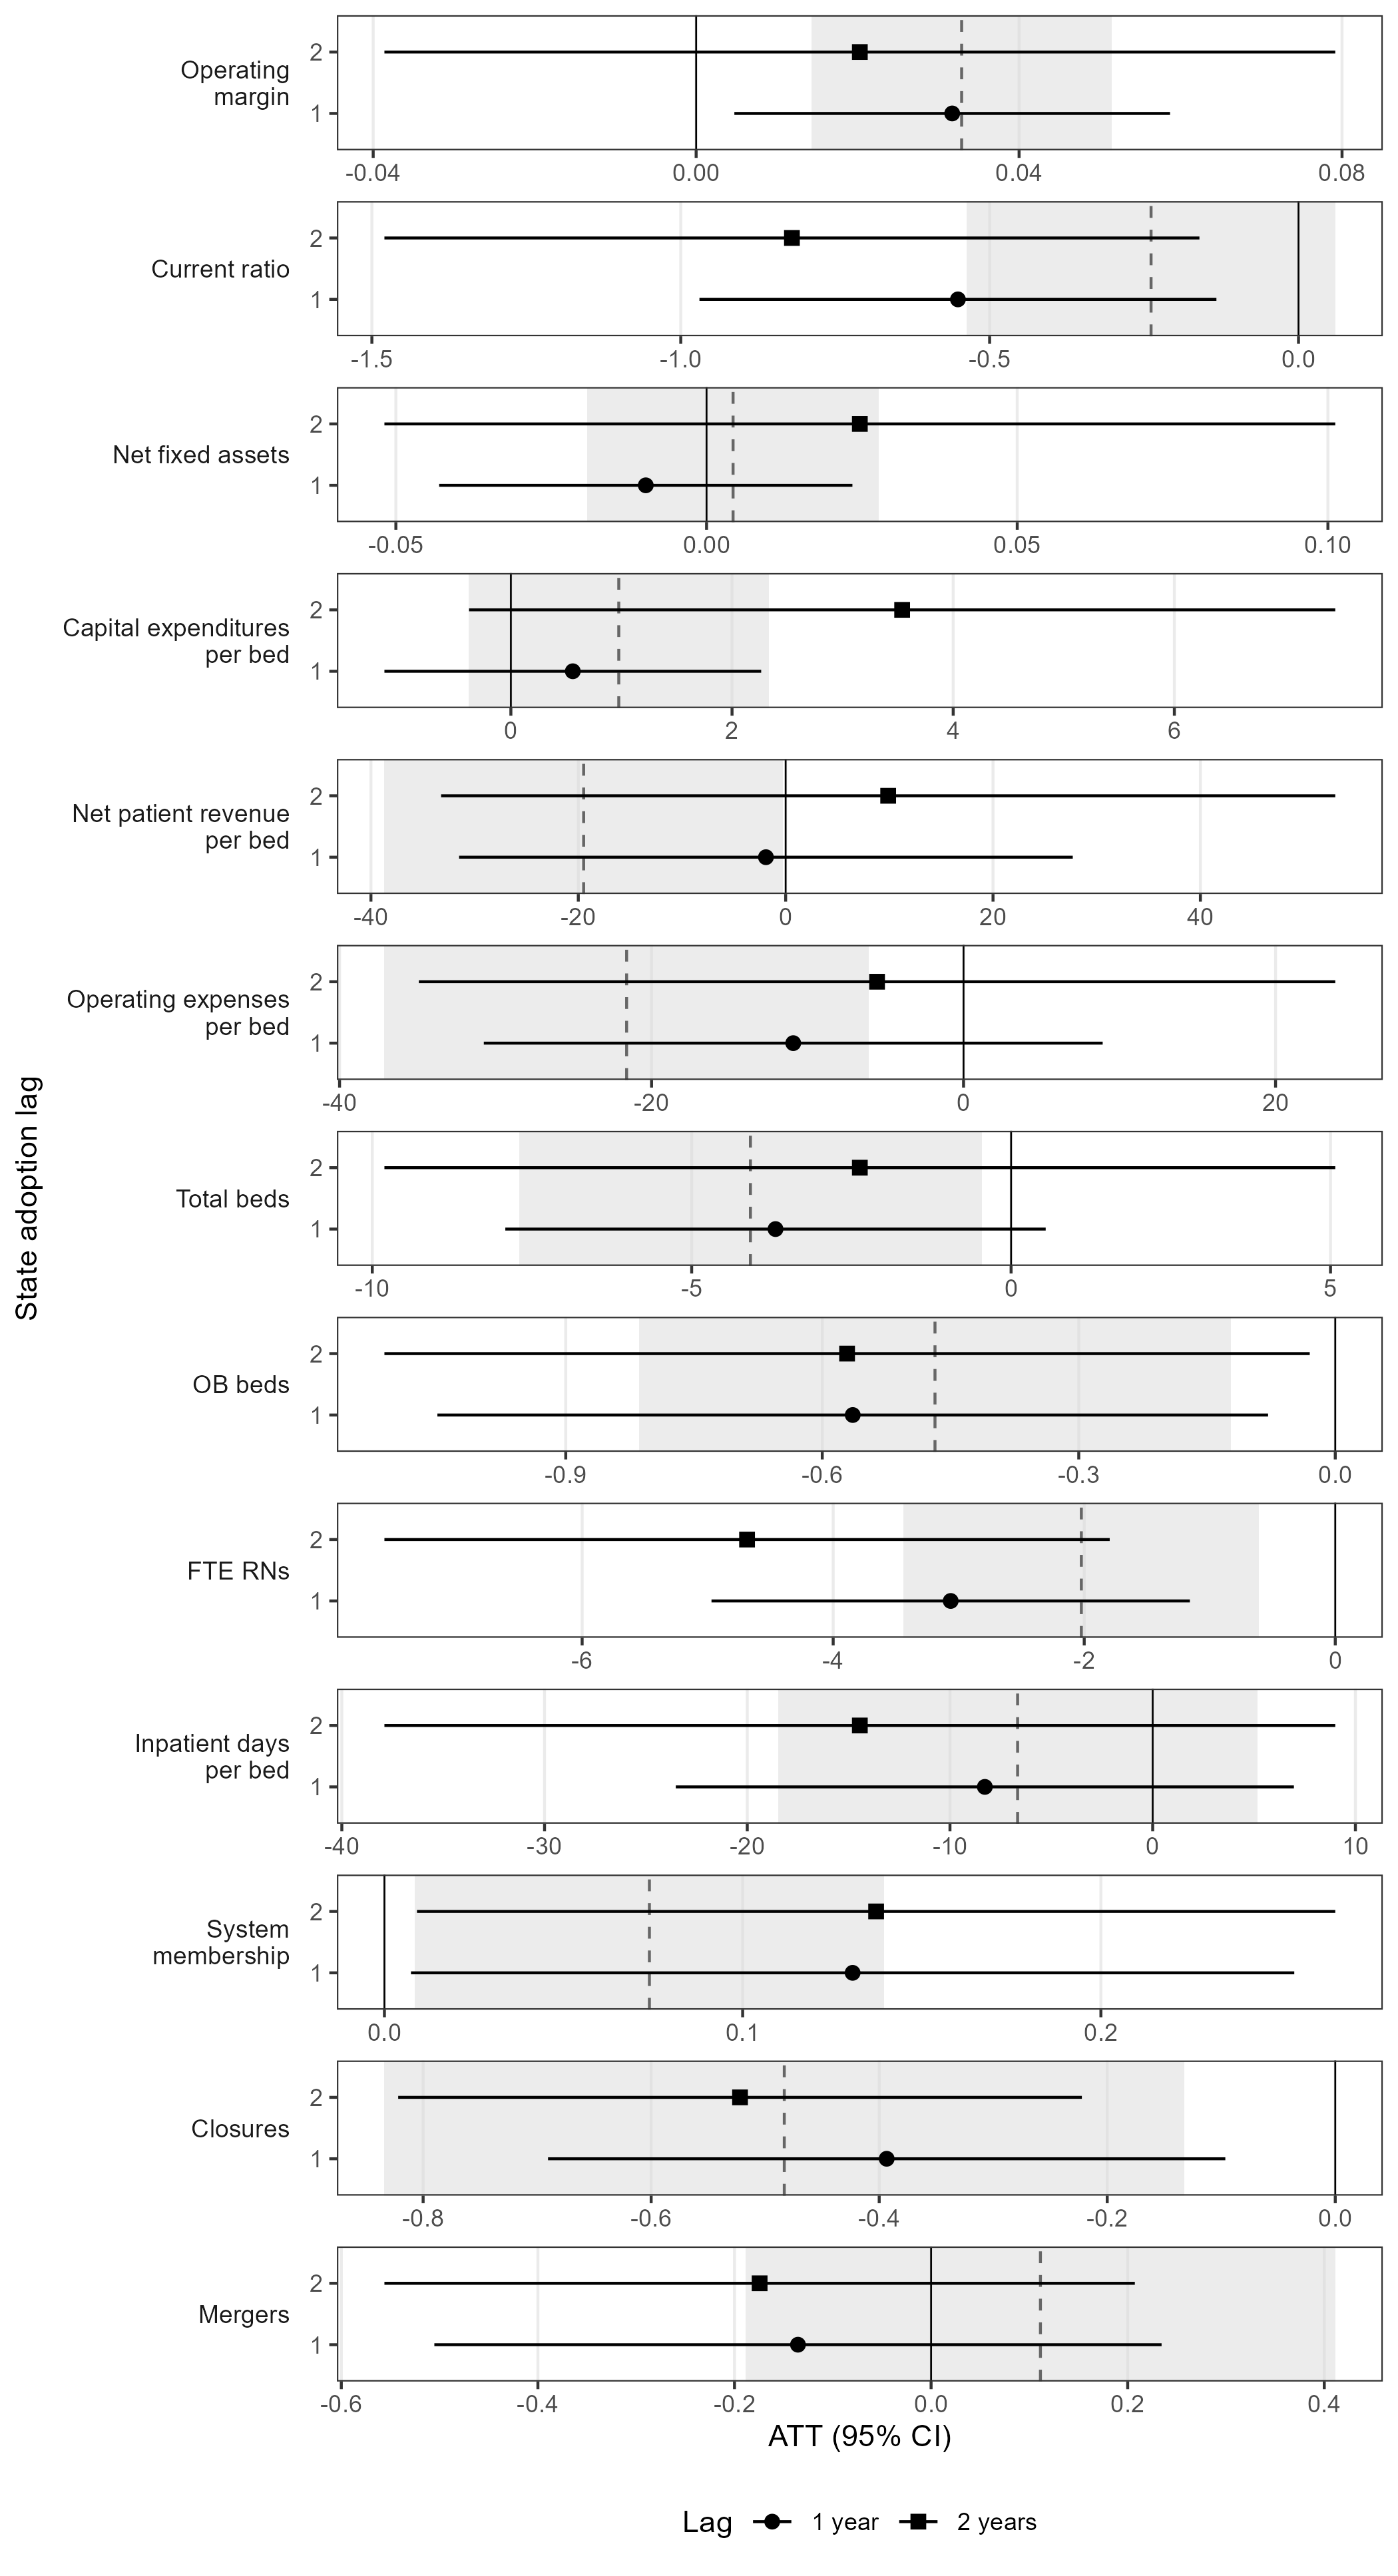
\includegraphics[width=\textwidth, height=0.8\textheight, keepaspectratio]{../results/statecut-sensitivity.png}
\end{minipage}
\end{figure}

\clearpage

\begin{figure}[!h]
\centering
\begin{minipage}[h]{6in}
\caption[Post-Period Sensitivity]{\textbf{SDID Estimates by Post-Period Length}\footnote{The shaded band spans the baseline (5-year post-period) 95\% confidence interval; the dashed line marks the baseline point estimate. Points show SDID ATTs at post-period lengths of 5, 4, 3, and 2 years, with 95\% confidence intervals.}}
\label{fig:postperiod-sensitivity}
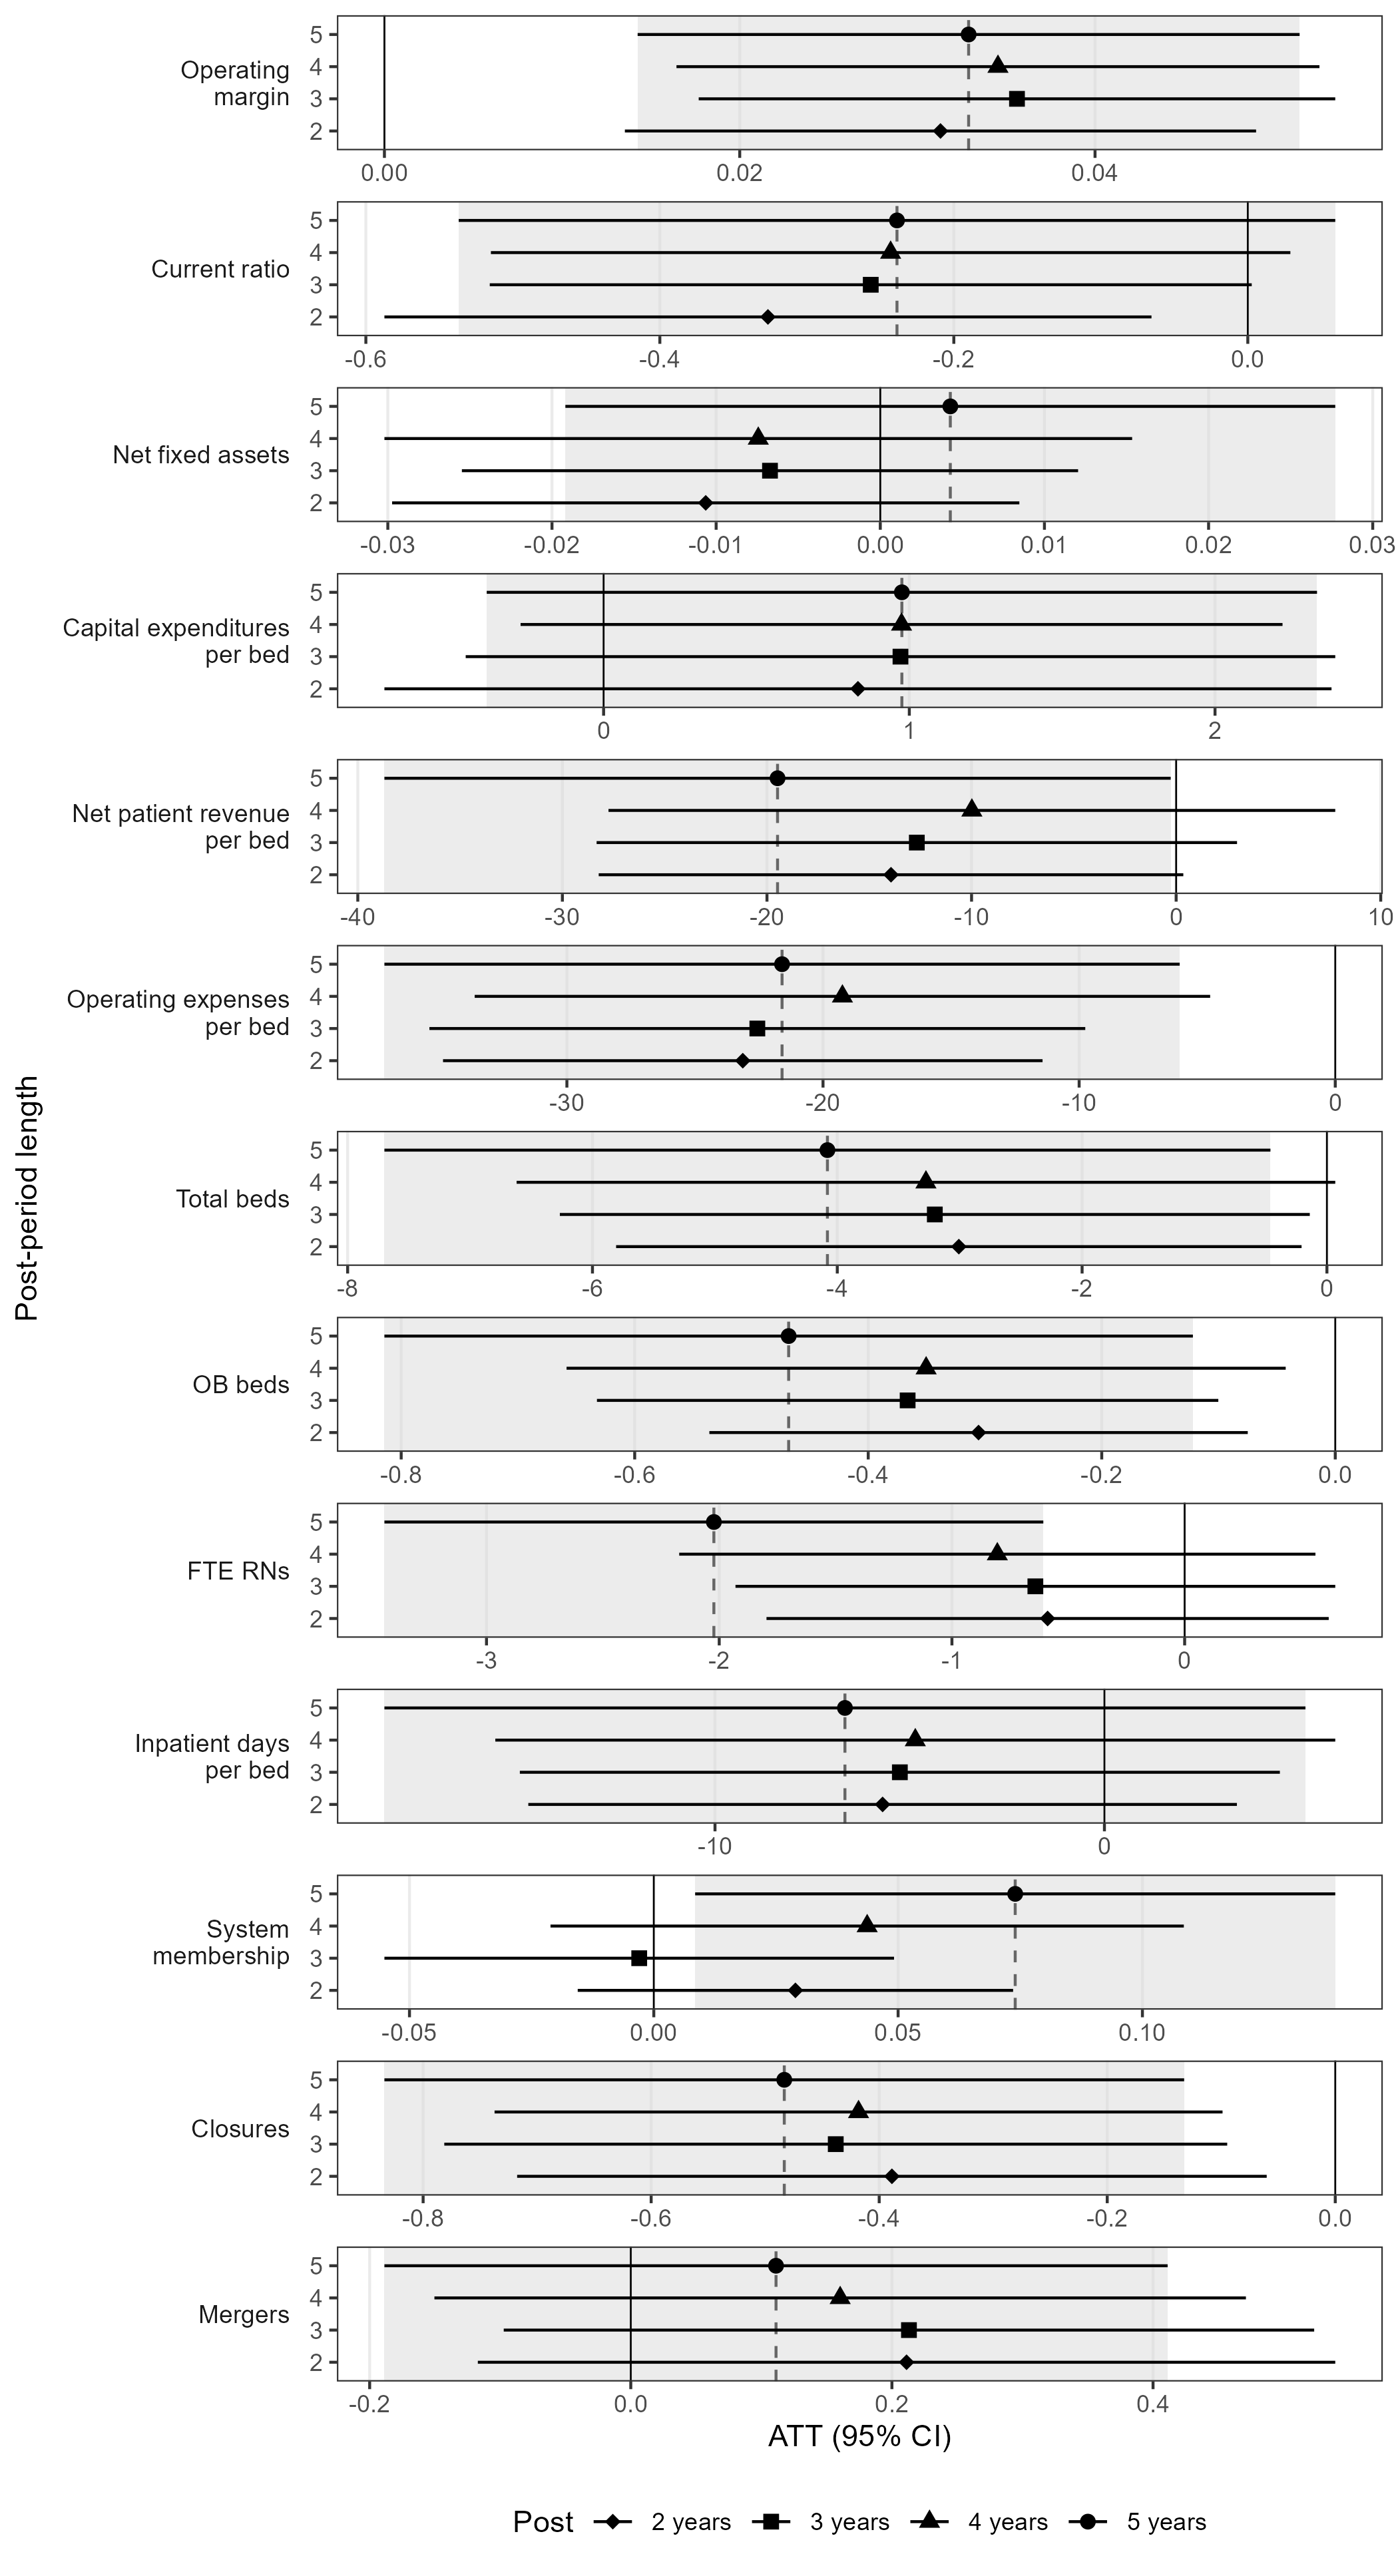
\includegraphics[width=\textwidth, height=0.8\textheight, keepaspectratio]{../results/control-timing-postperiod.png}
\end{minipage}
\end{figure}

\clearpage

\begin{figure}[!h]
\centering
\begin{minipage}[h]{6in}
\caption[Excluding Immediate Adopters]{\textbf{SDID Estimates Excluding Immediate Adopters}\footnote{The shaded band spans the baseline 95\% confidence interval; the dashed line marks the baseline point estimate. Points show SDID ATTs after dropping hospitals that converted to CAH in the same year their state first implemented the program (121 of 1,466 treated hospitals).}}
\label{fig:noimmediate-sensitivity}
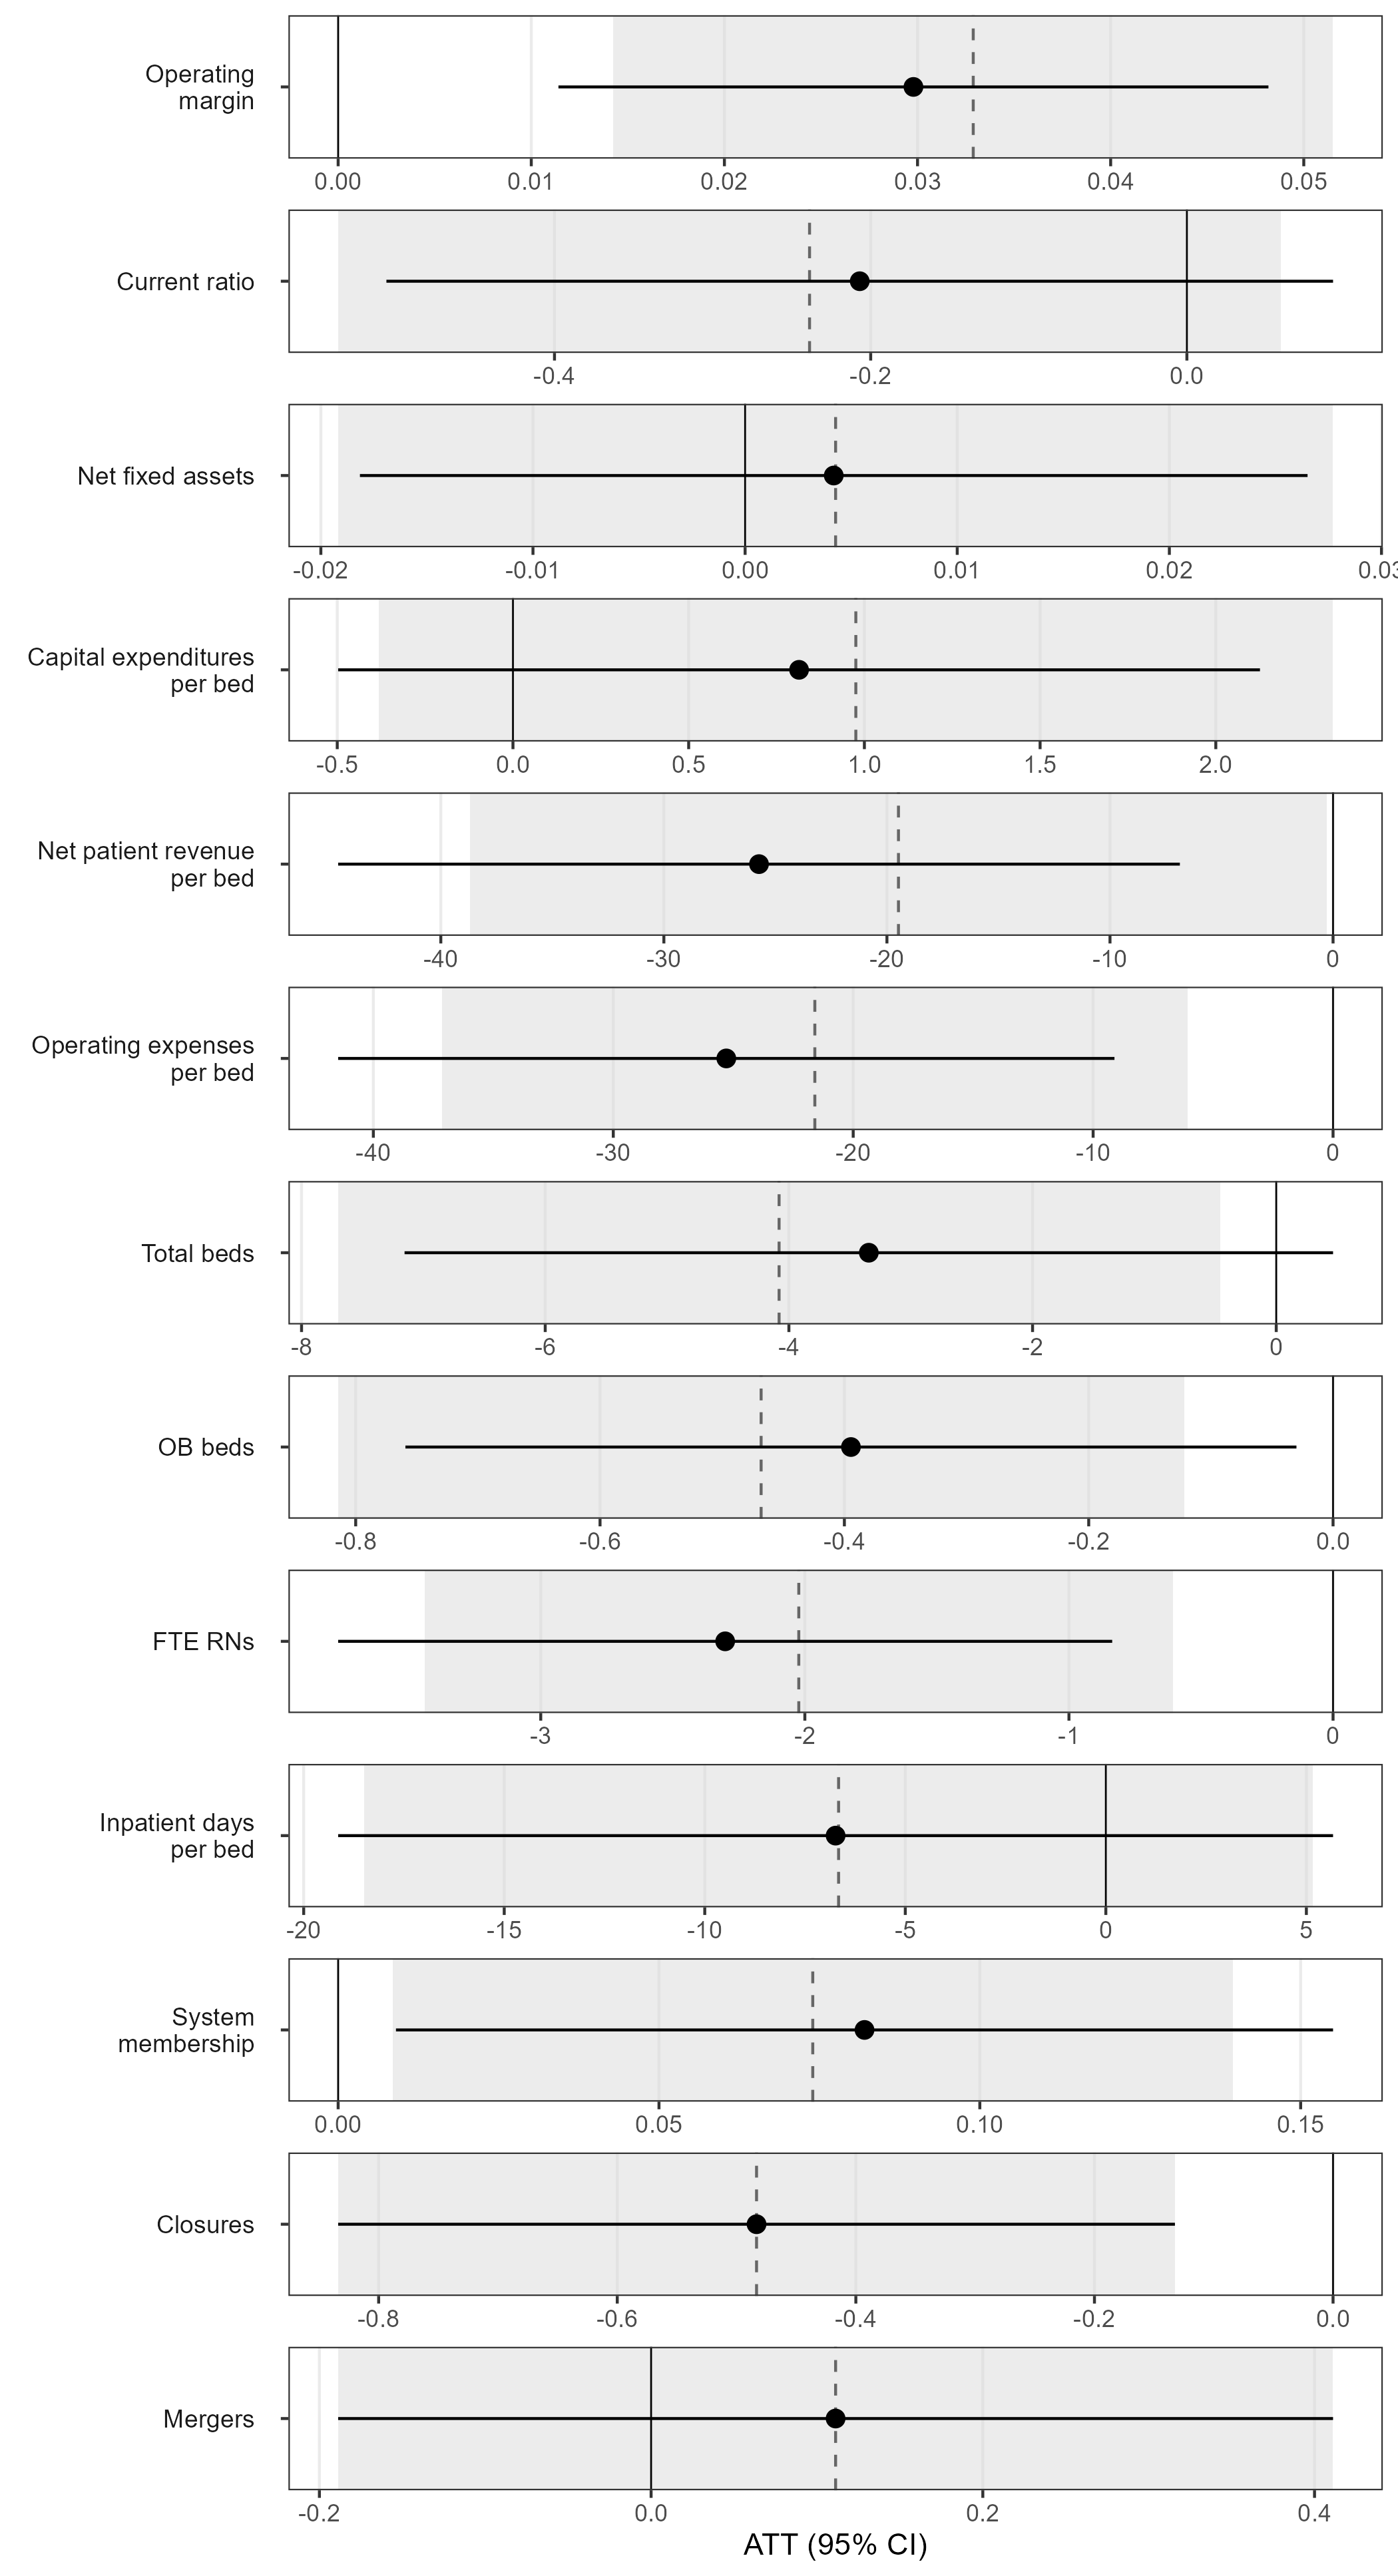
\includegraphics[width=\textwidth, height=0.8\textheight, keepaspectratio]{../results/control-timing-noimmediate.png}
\end{minipage}
\end{figure}

\clearpage

\begin{figure}[!h]
\centering
\begin{minipage}[h]{6in}
\caption[Excluding Never-Treated States]{\textbf{SDID Estimates Excluding Never-Treated States}\footnote{The shaded band spans the baseline 95\% confidence interval; the dashed line marks the baseline point estimate. Points show SDID ATTs after dropping all hospitals in states that never adopted CAH designation (Connecticut, New Jersey, and Rhode Island; 10 hospitals with $\leq 50$ beds).}}
\label{fig:nonever-sensitivity}
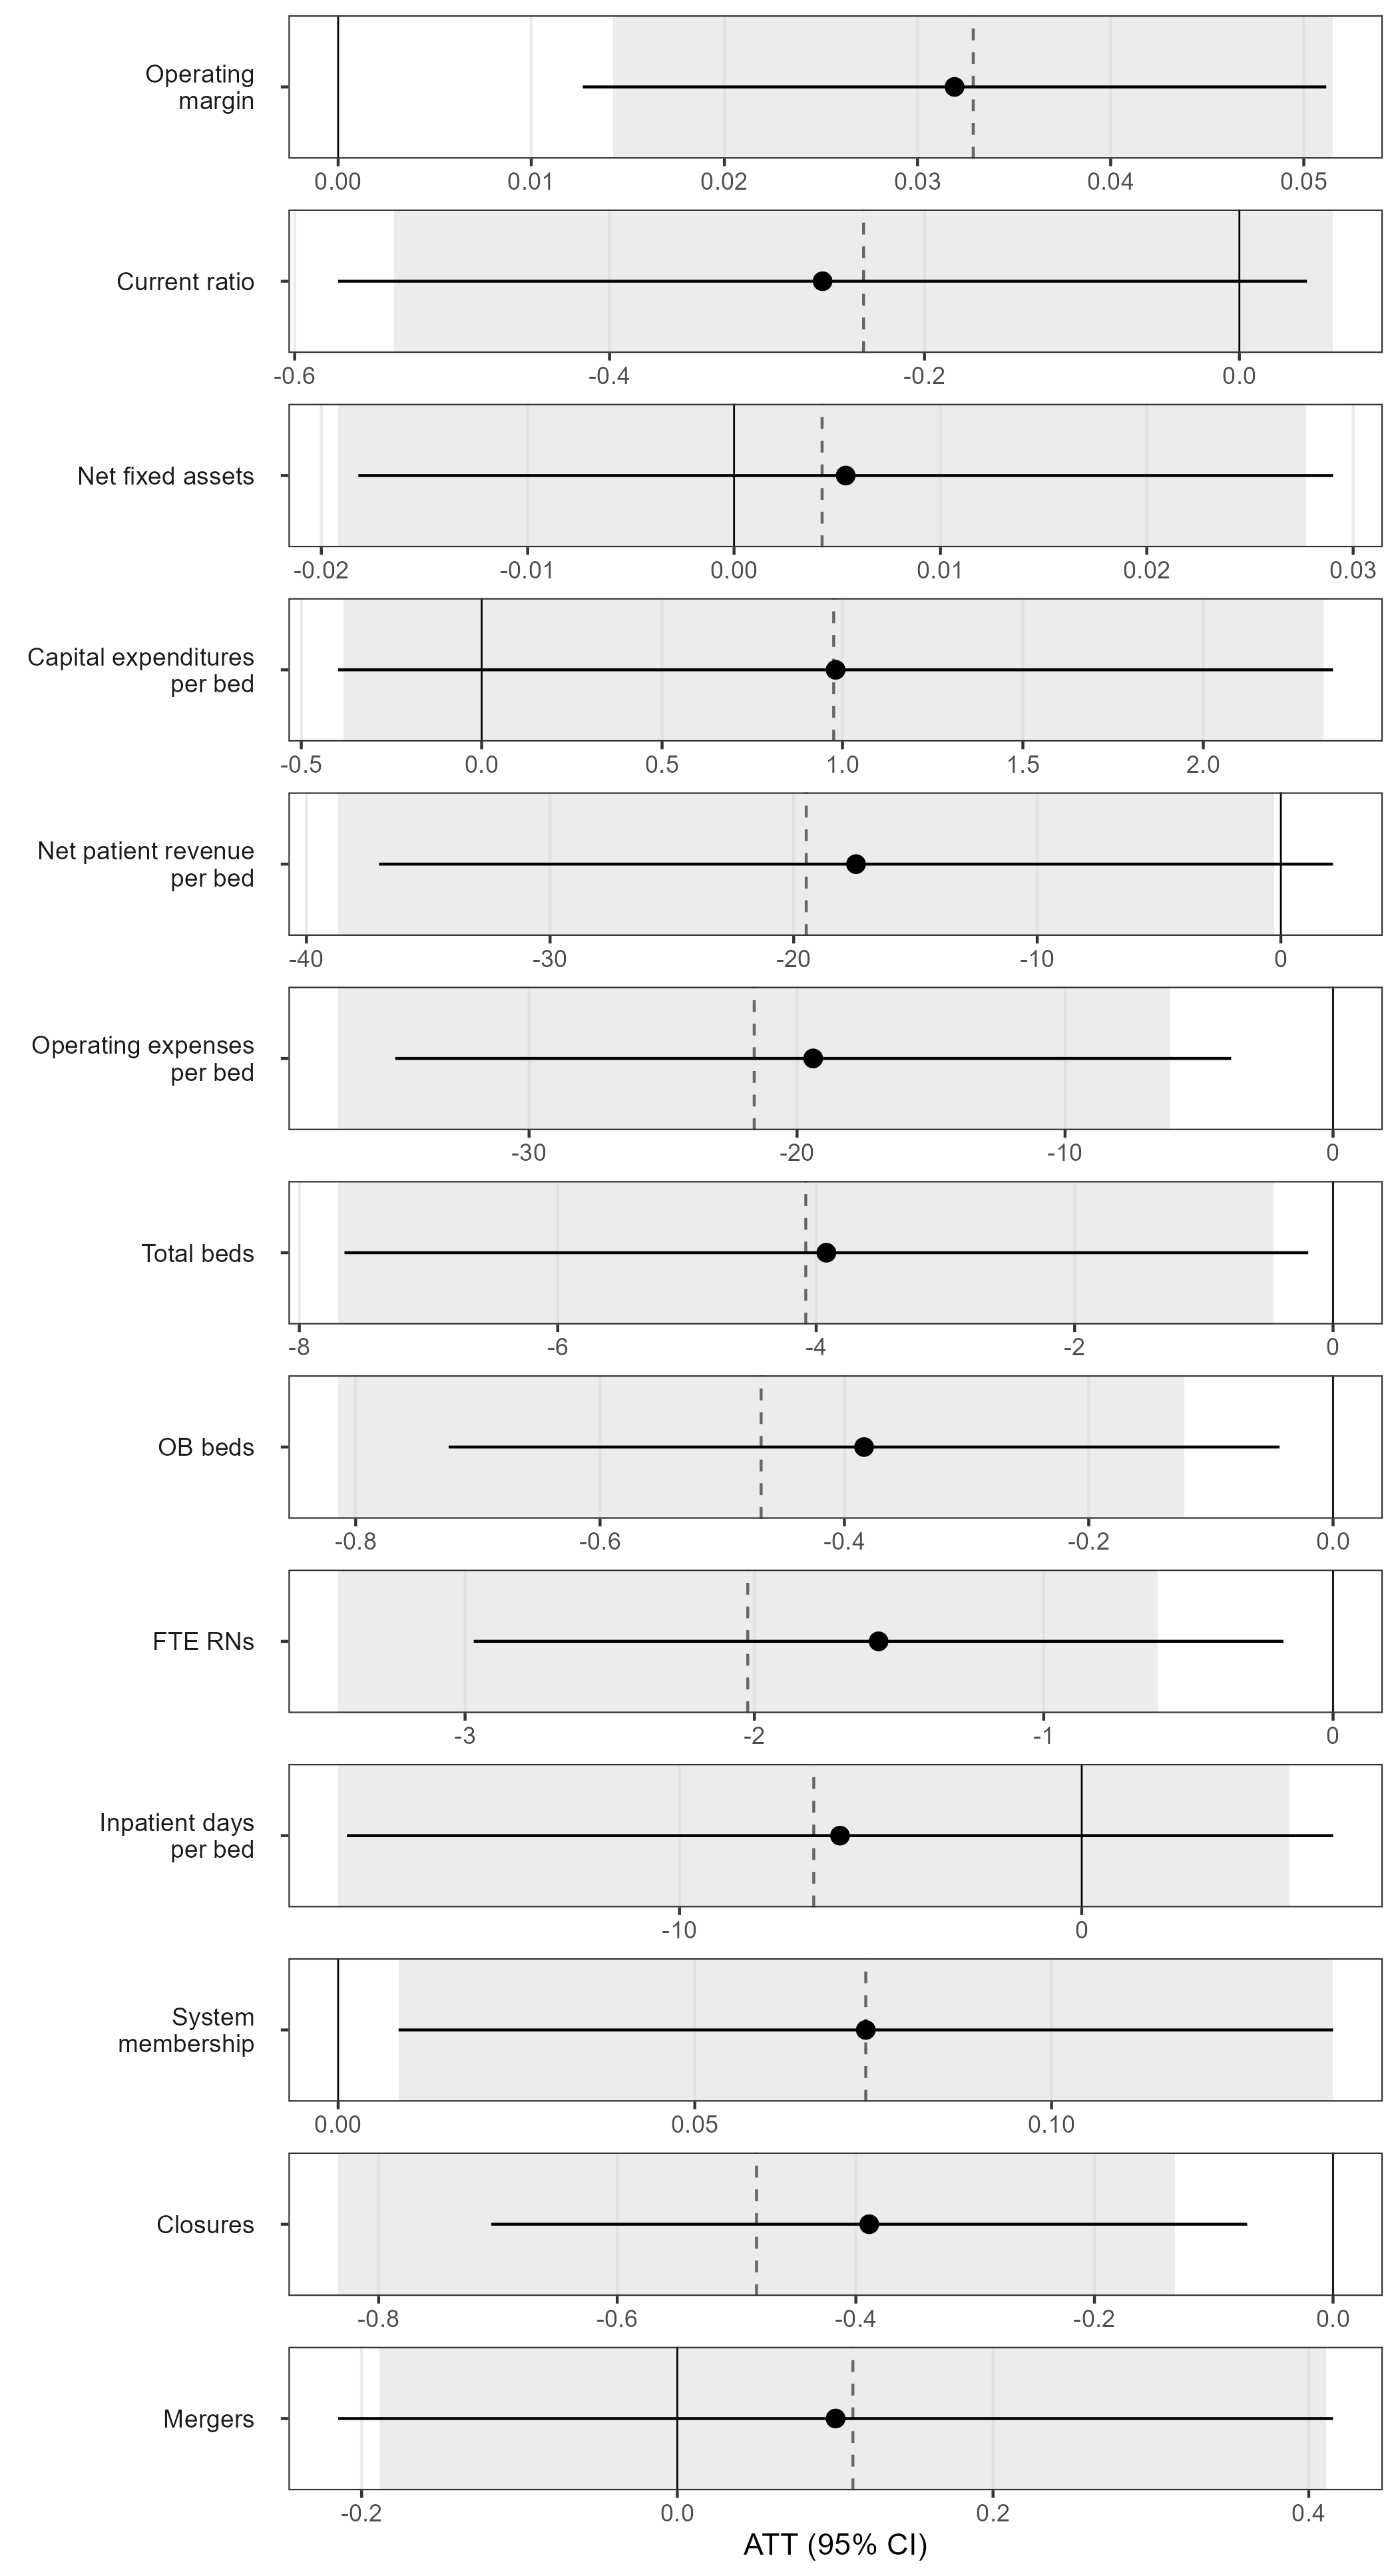
\includegraphics[width=\textwidth, height=0.8\textheight, keepaspectratio]{../results/control-timing-nonever.png}
\end{minipage}
\end{figure}

\clearpage

\begin{figure}[!h]
\centering
\begin{minipage}[h]{6in}
\caption[Bed Size Cutoff Sensitivity]{\textbf{SDID Estimates by Bed Size Cutoff}\footnote{The shaded band spans the baseline (50-bed cutoff) 95\% confidence interval; the dashed line marks the baseline point estimate. Points show SDID ATTs at 25-bed and 75-bed cutoffs, with 95\% confidence intervals. Cohort-cutoff combinations with fewer than 5 control hospitals in the balanced panel are excluded.}}
\label{fig:bedcut-sensitivity}
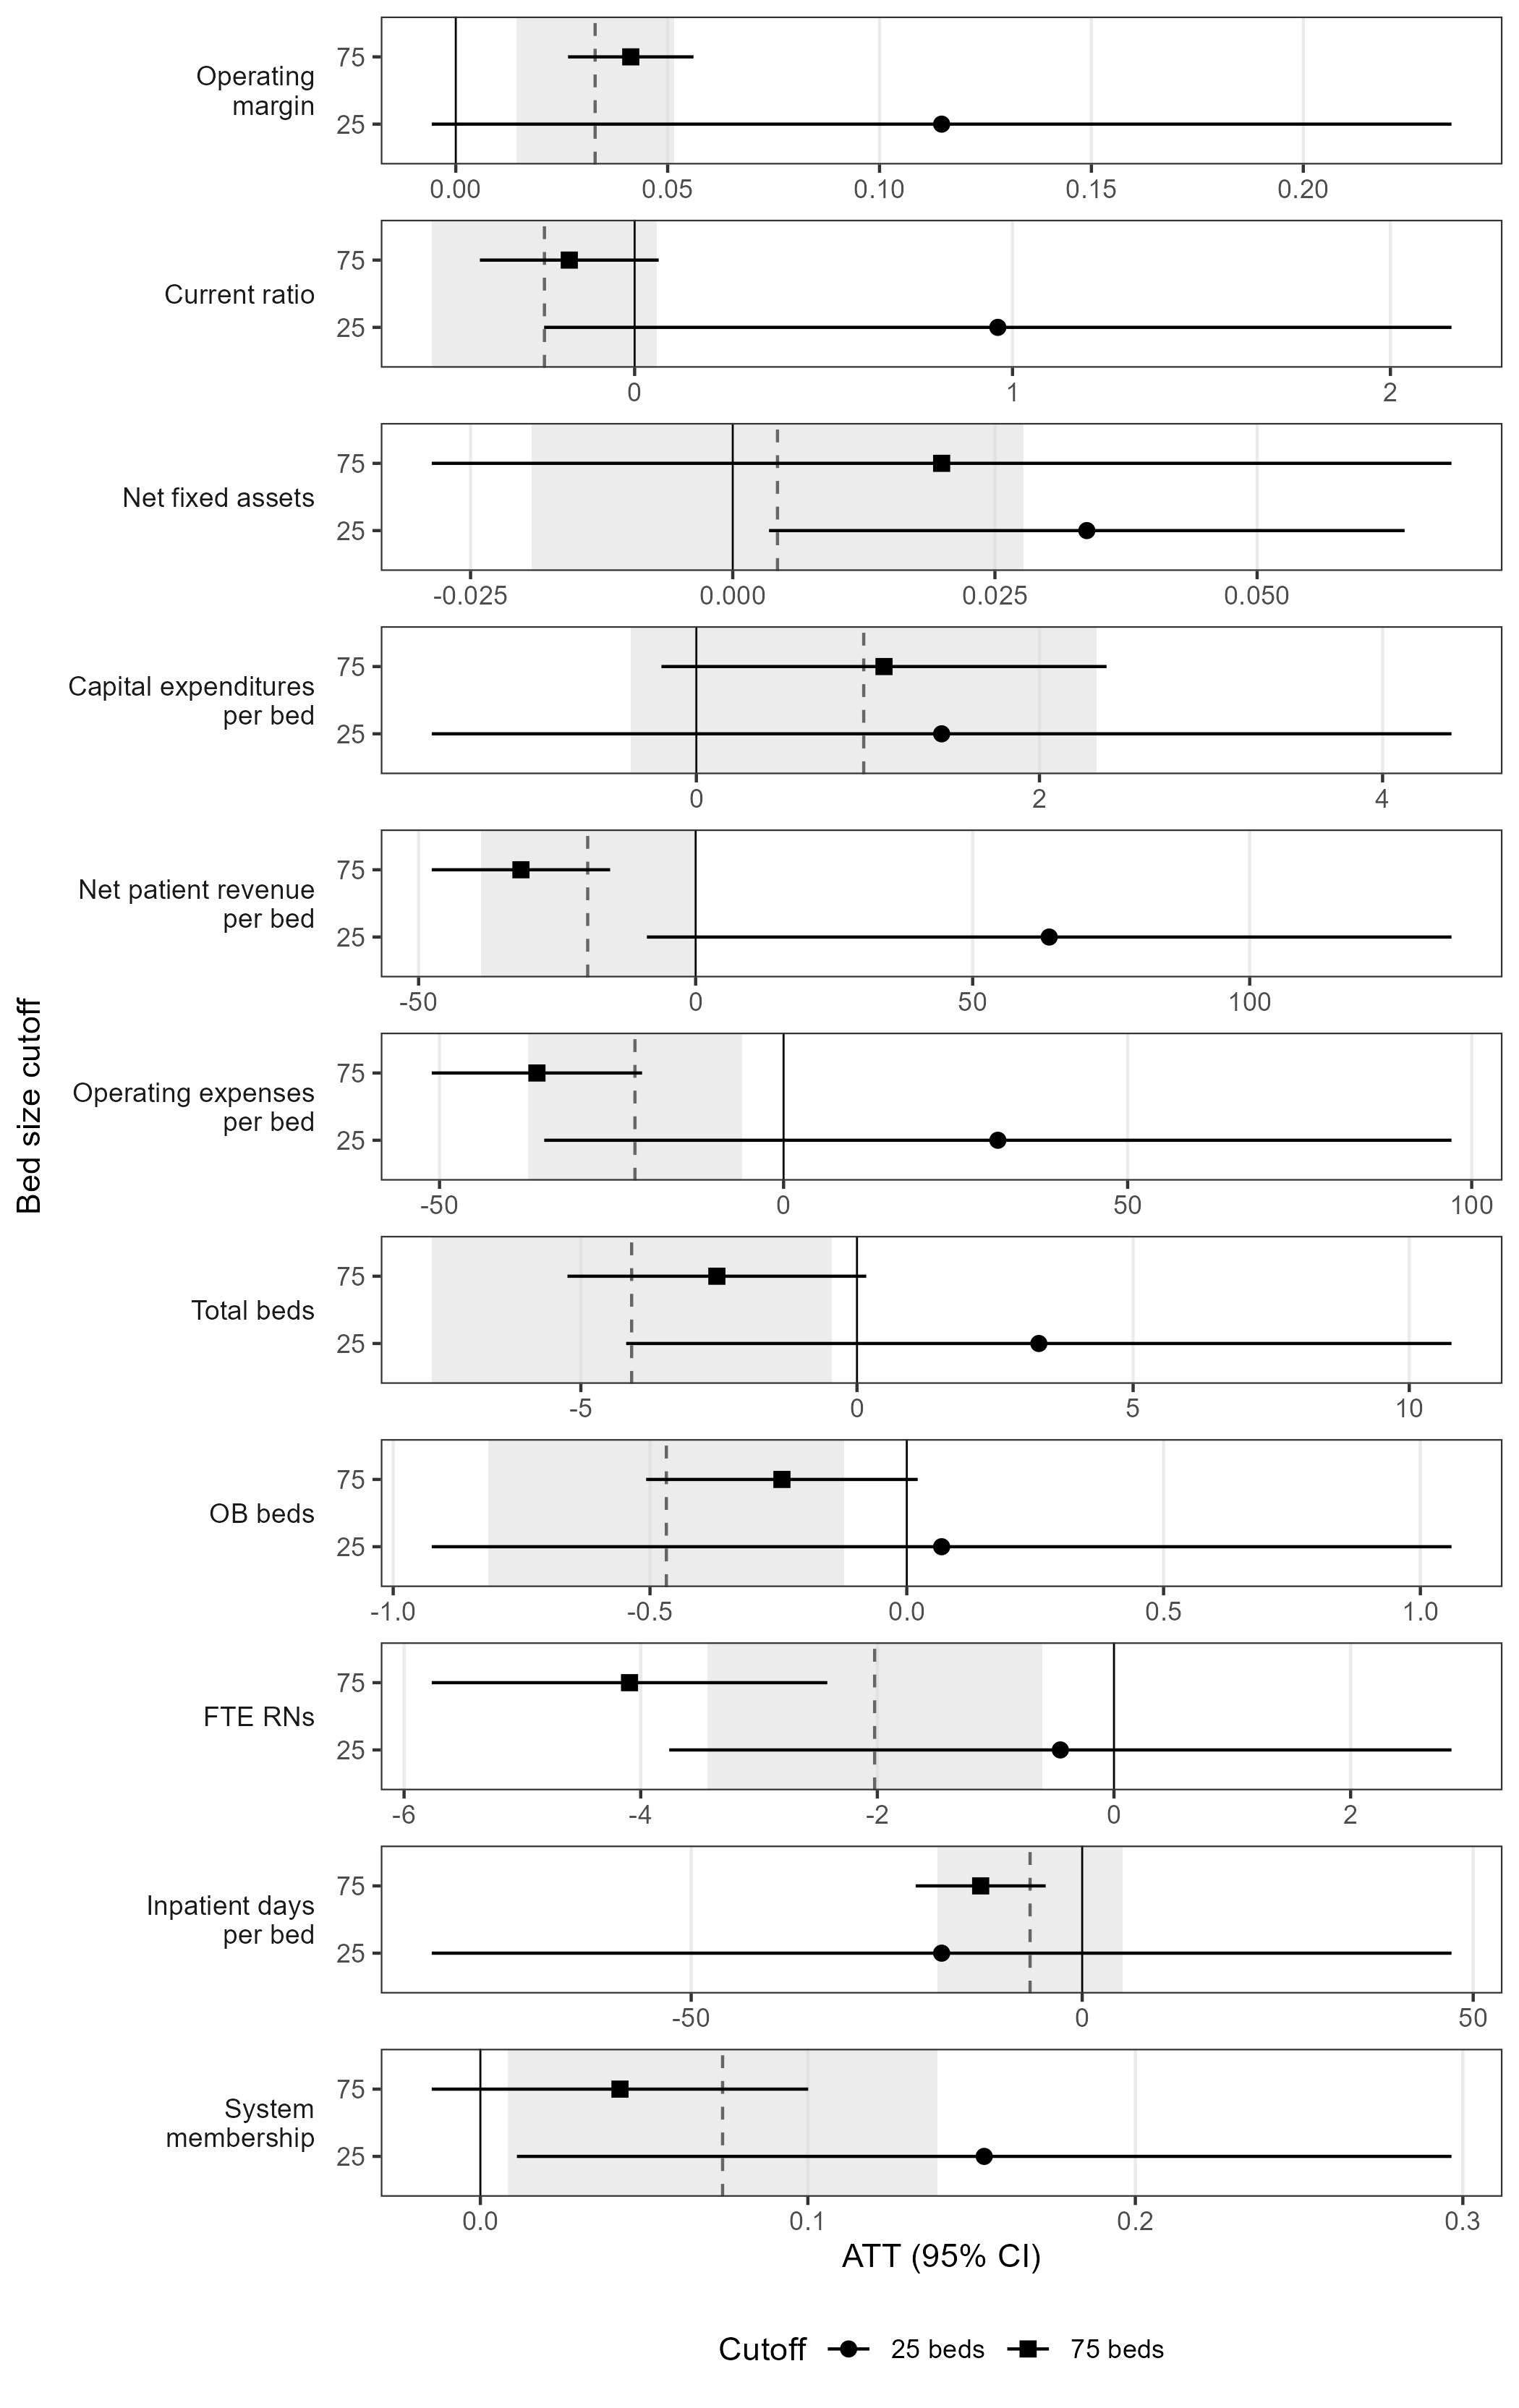
\includegraphics[width=\textwidth, height=0.85\textheight, keepaspectratio]{../results/bedcut-sensitivity.png}
\end{minipage}
\end{figure}

\clearpage

%%% Alternative Estimator Figures

\begin{figure}[!h]
\centering
\begin{minipage}[h]{6in}
\caption[CS Event Studies: Financial]{\textbf{CS Event-Study Estimates: Financial Performance and Capital}\footnote{Callaway--Sant'Anna event-study estimates with 95\% confidence intervals by years relative to designation, state-timing design (cohorts 1999--2001), not-yet-treated control group, universal base period. Revenue and expense measures are in thousands of 2010 dollars per bed.}}
\label{fig:cs-financial}
\begin{tabular}{cc}
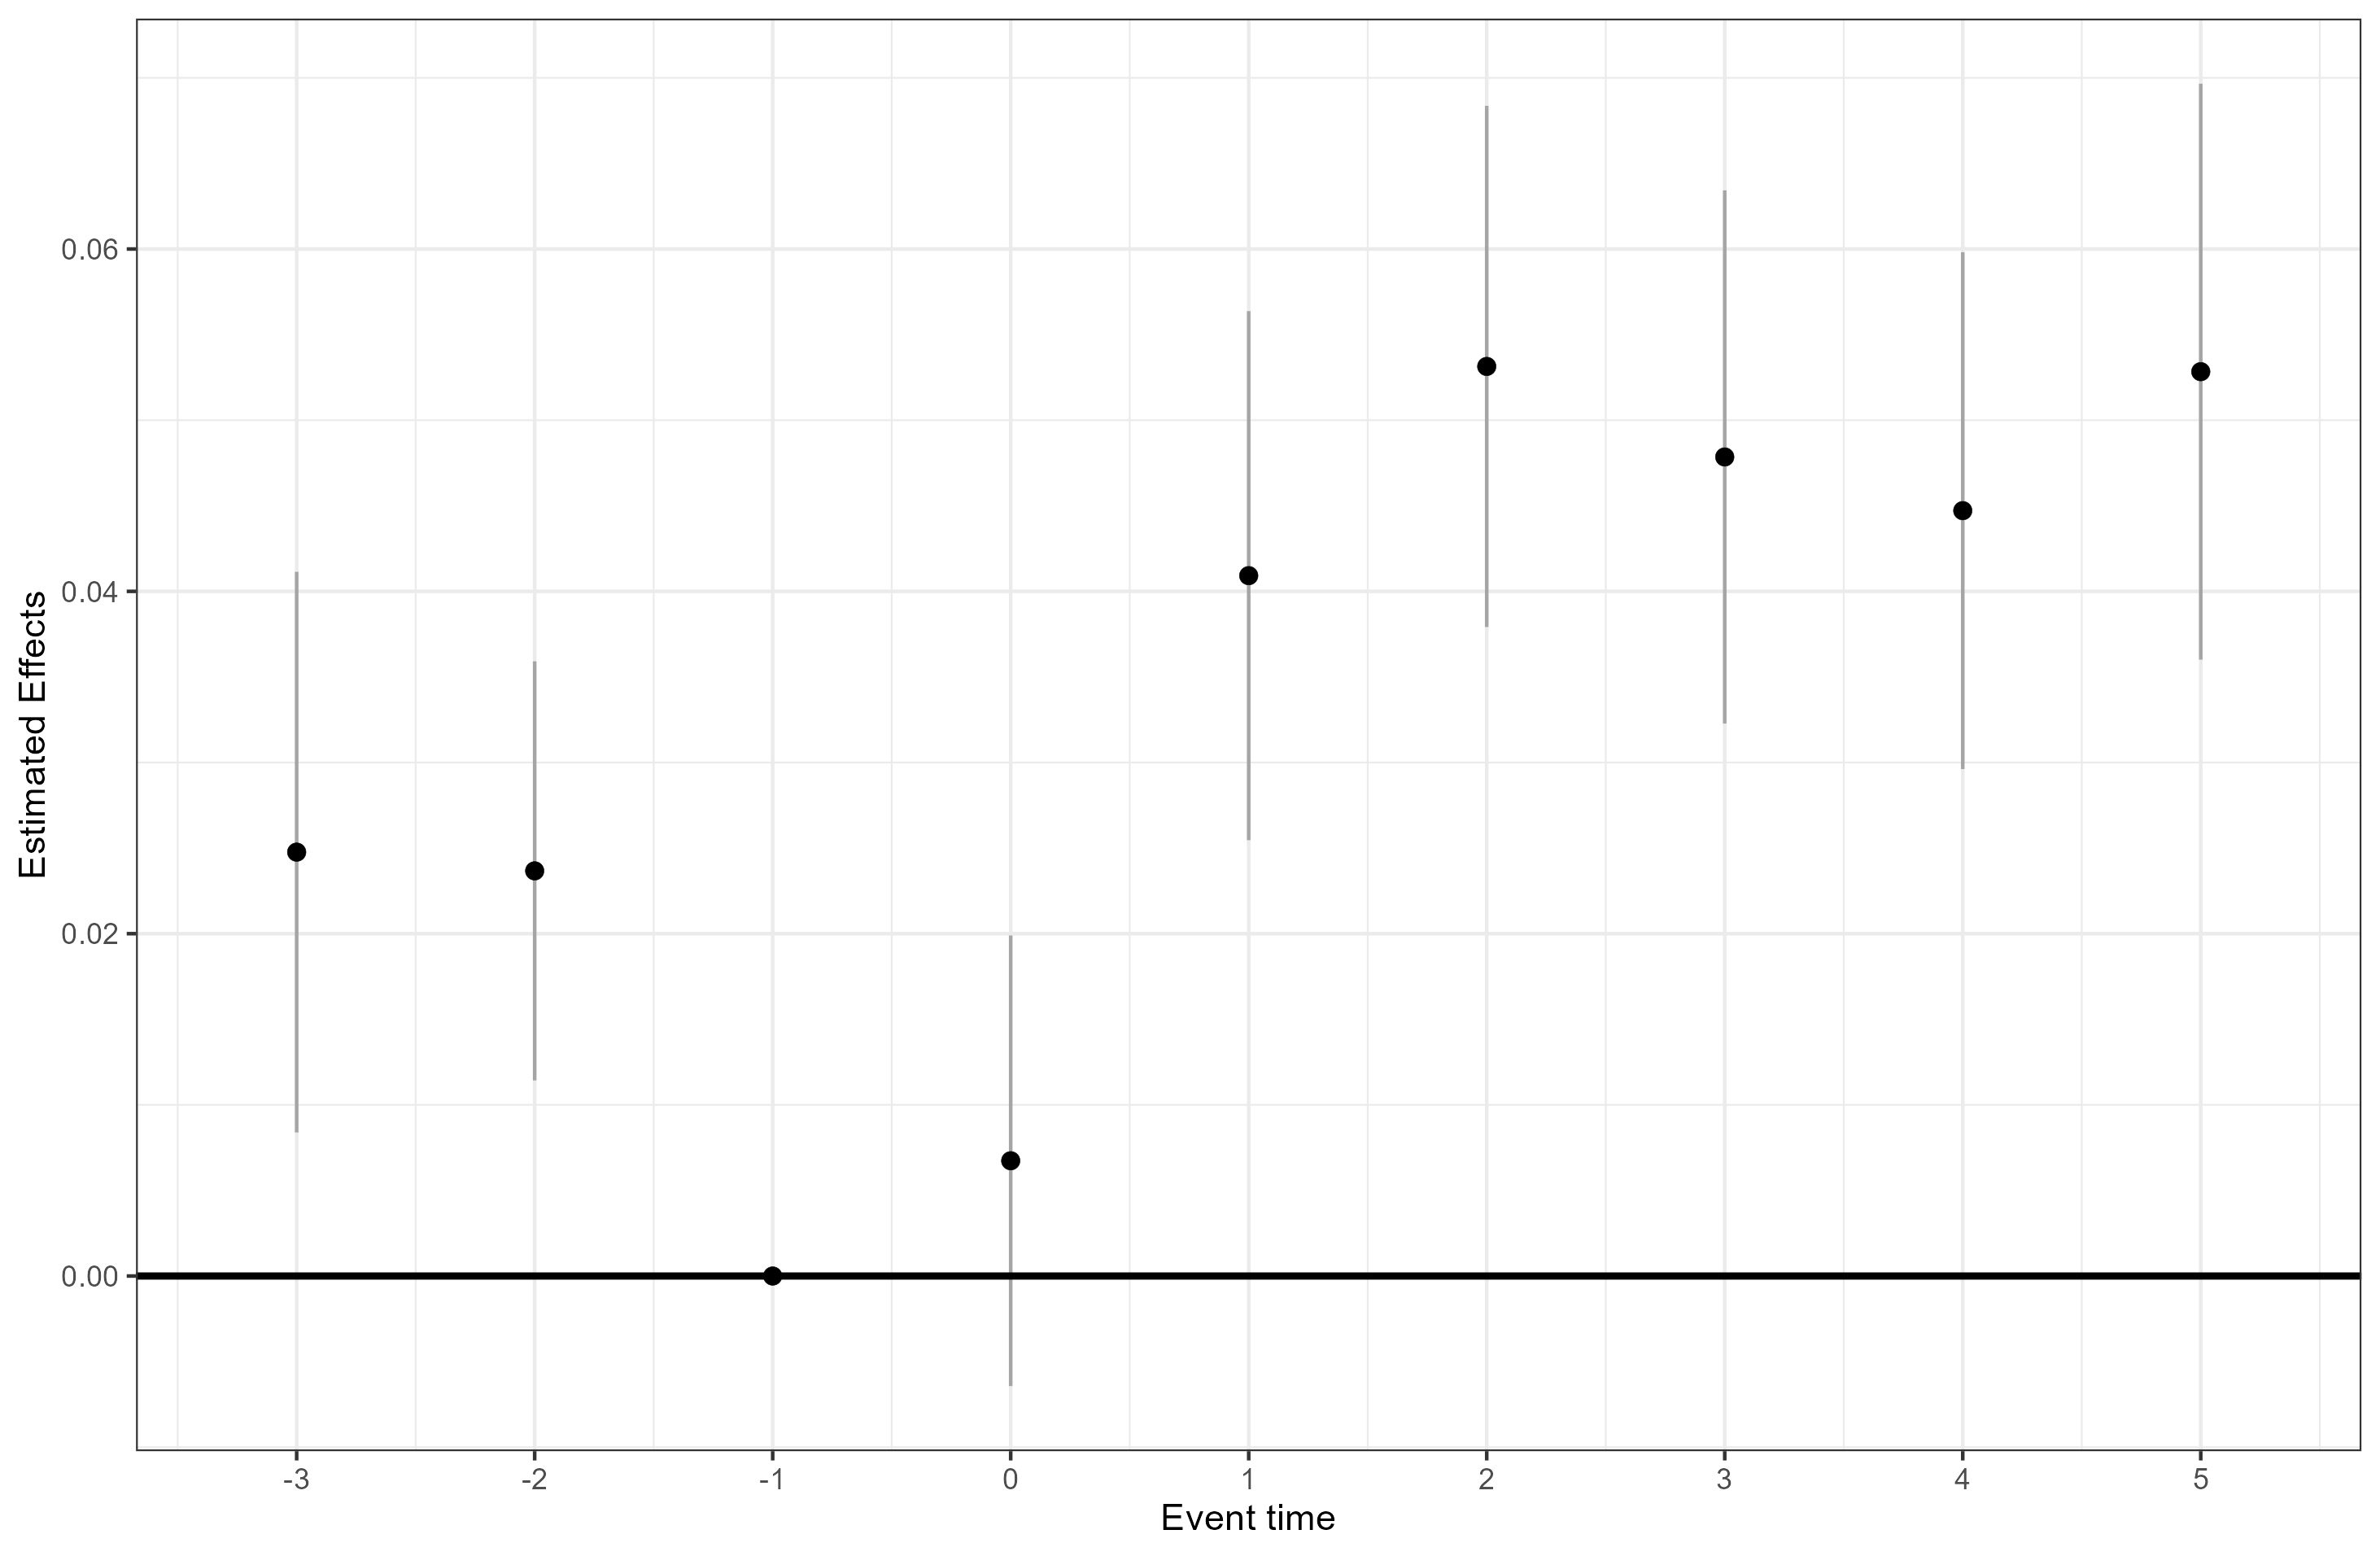
\includegraphics[width=0.48\textwidth]{../results/margin-cs.png} &
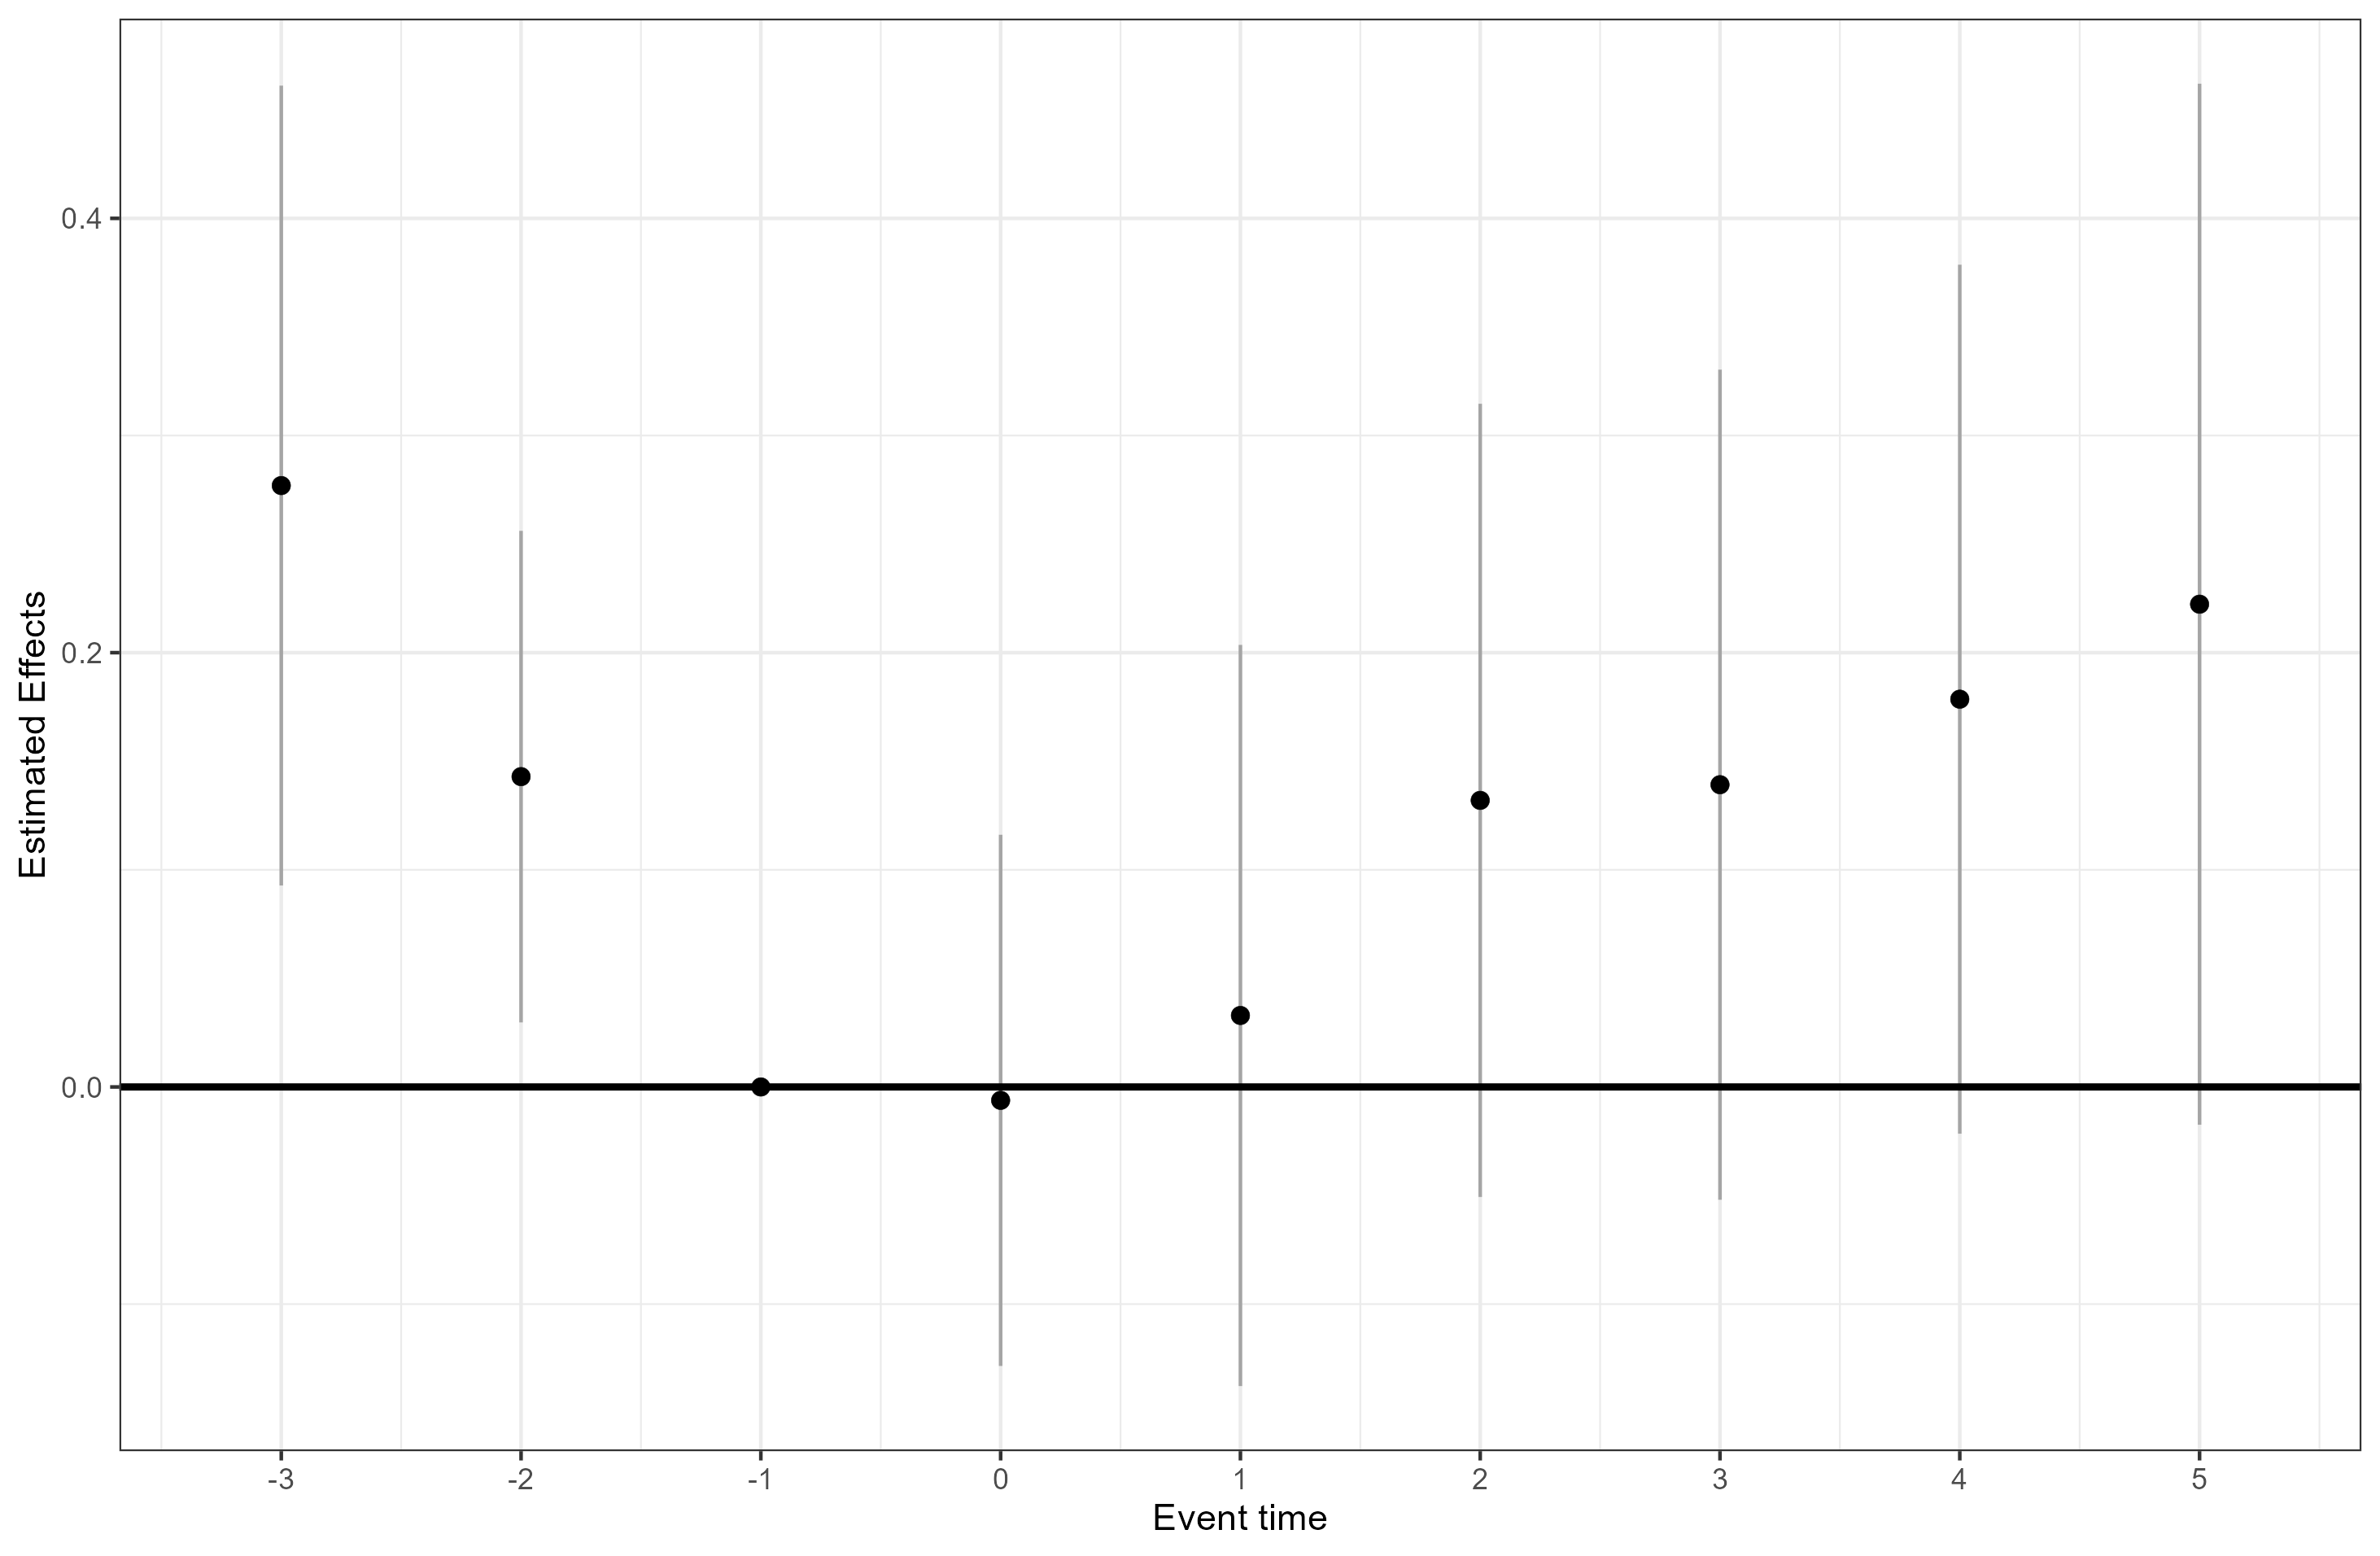
\includegraphics[width=0.48\textwidth]{../results/currentratio-cs.png} \\
\small (a) Operating Margin & \small (b) Current Ratio \\[0.5cm]
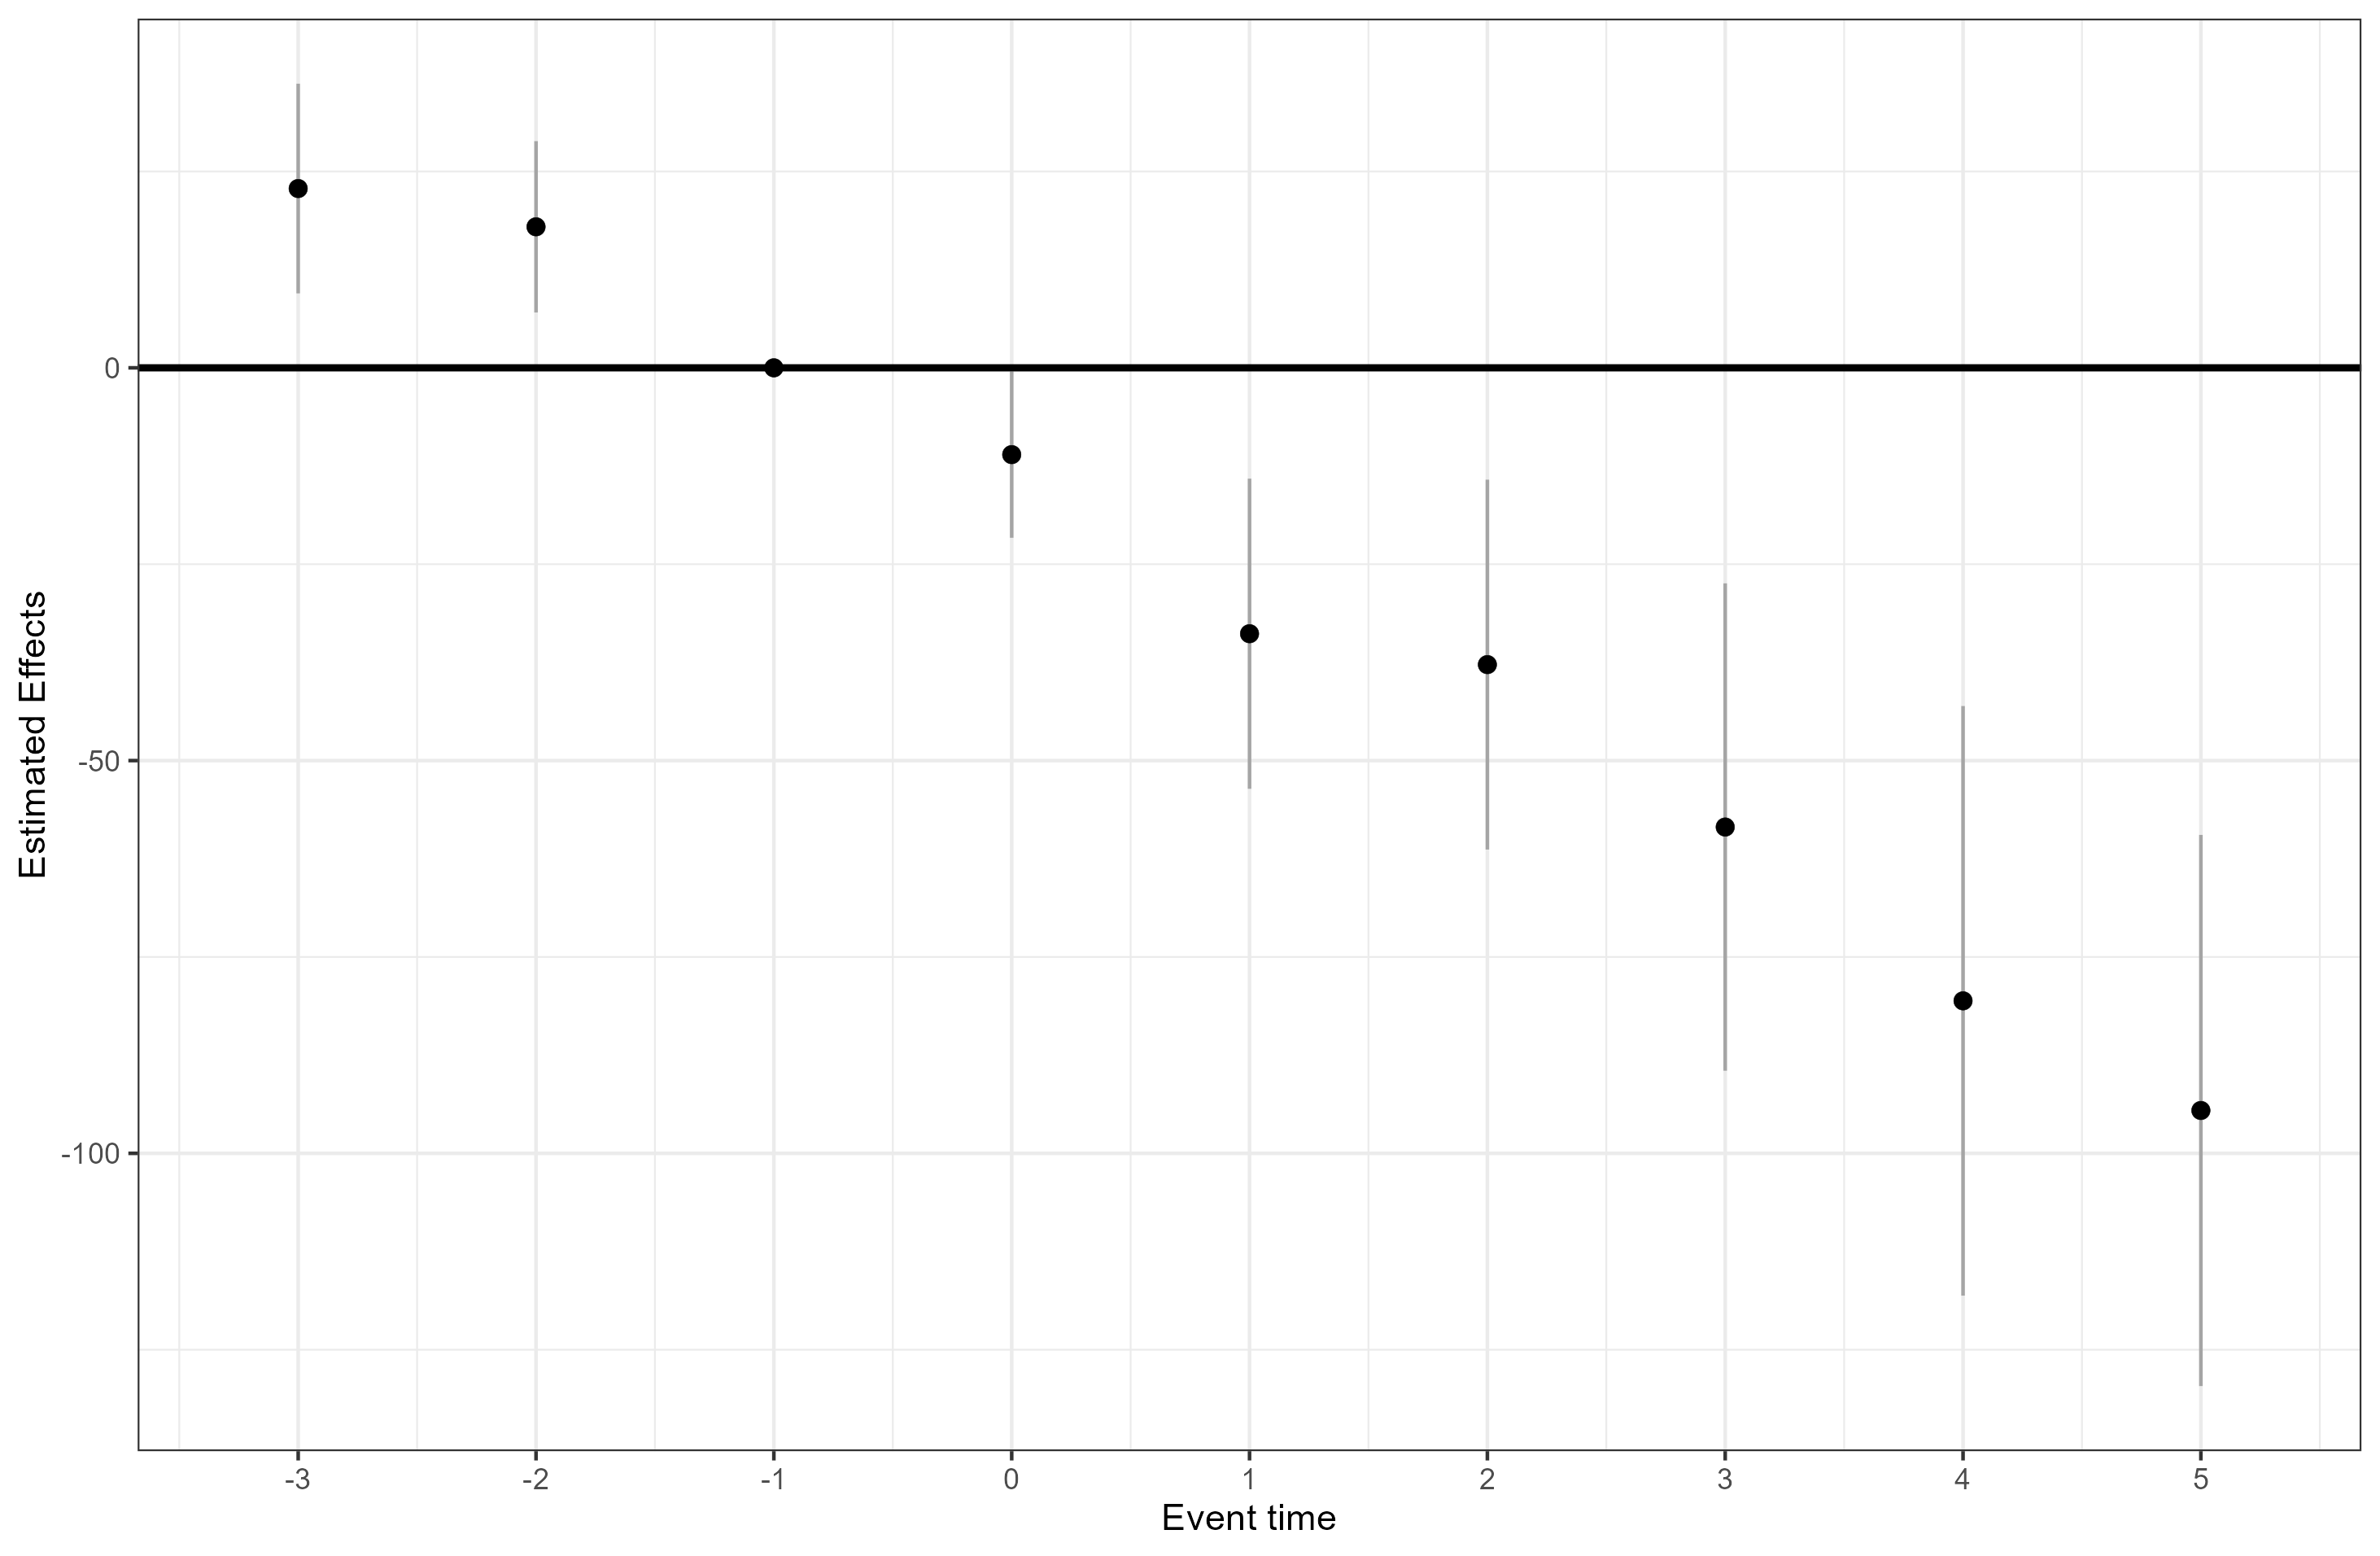
\includegraphics[width=0.48\textwidth]{../results/netpatrev-cs.png} &
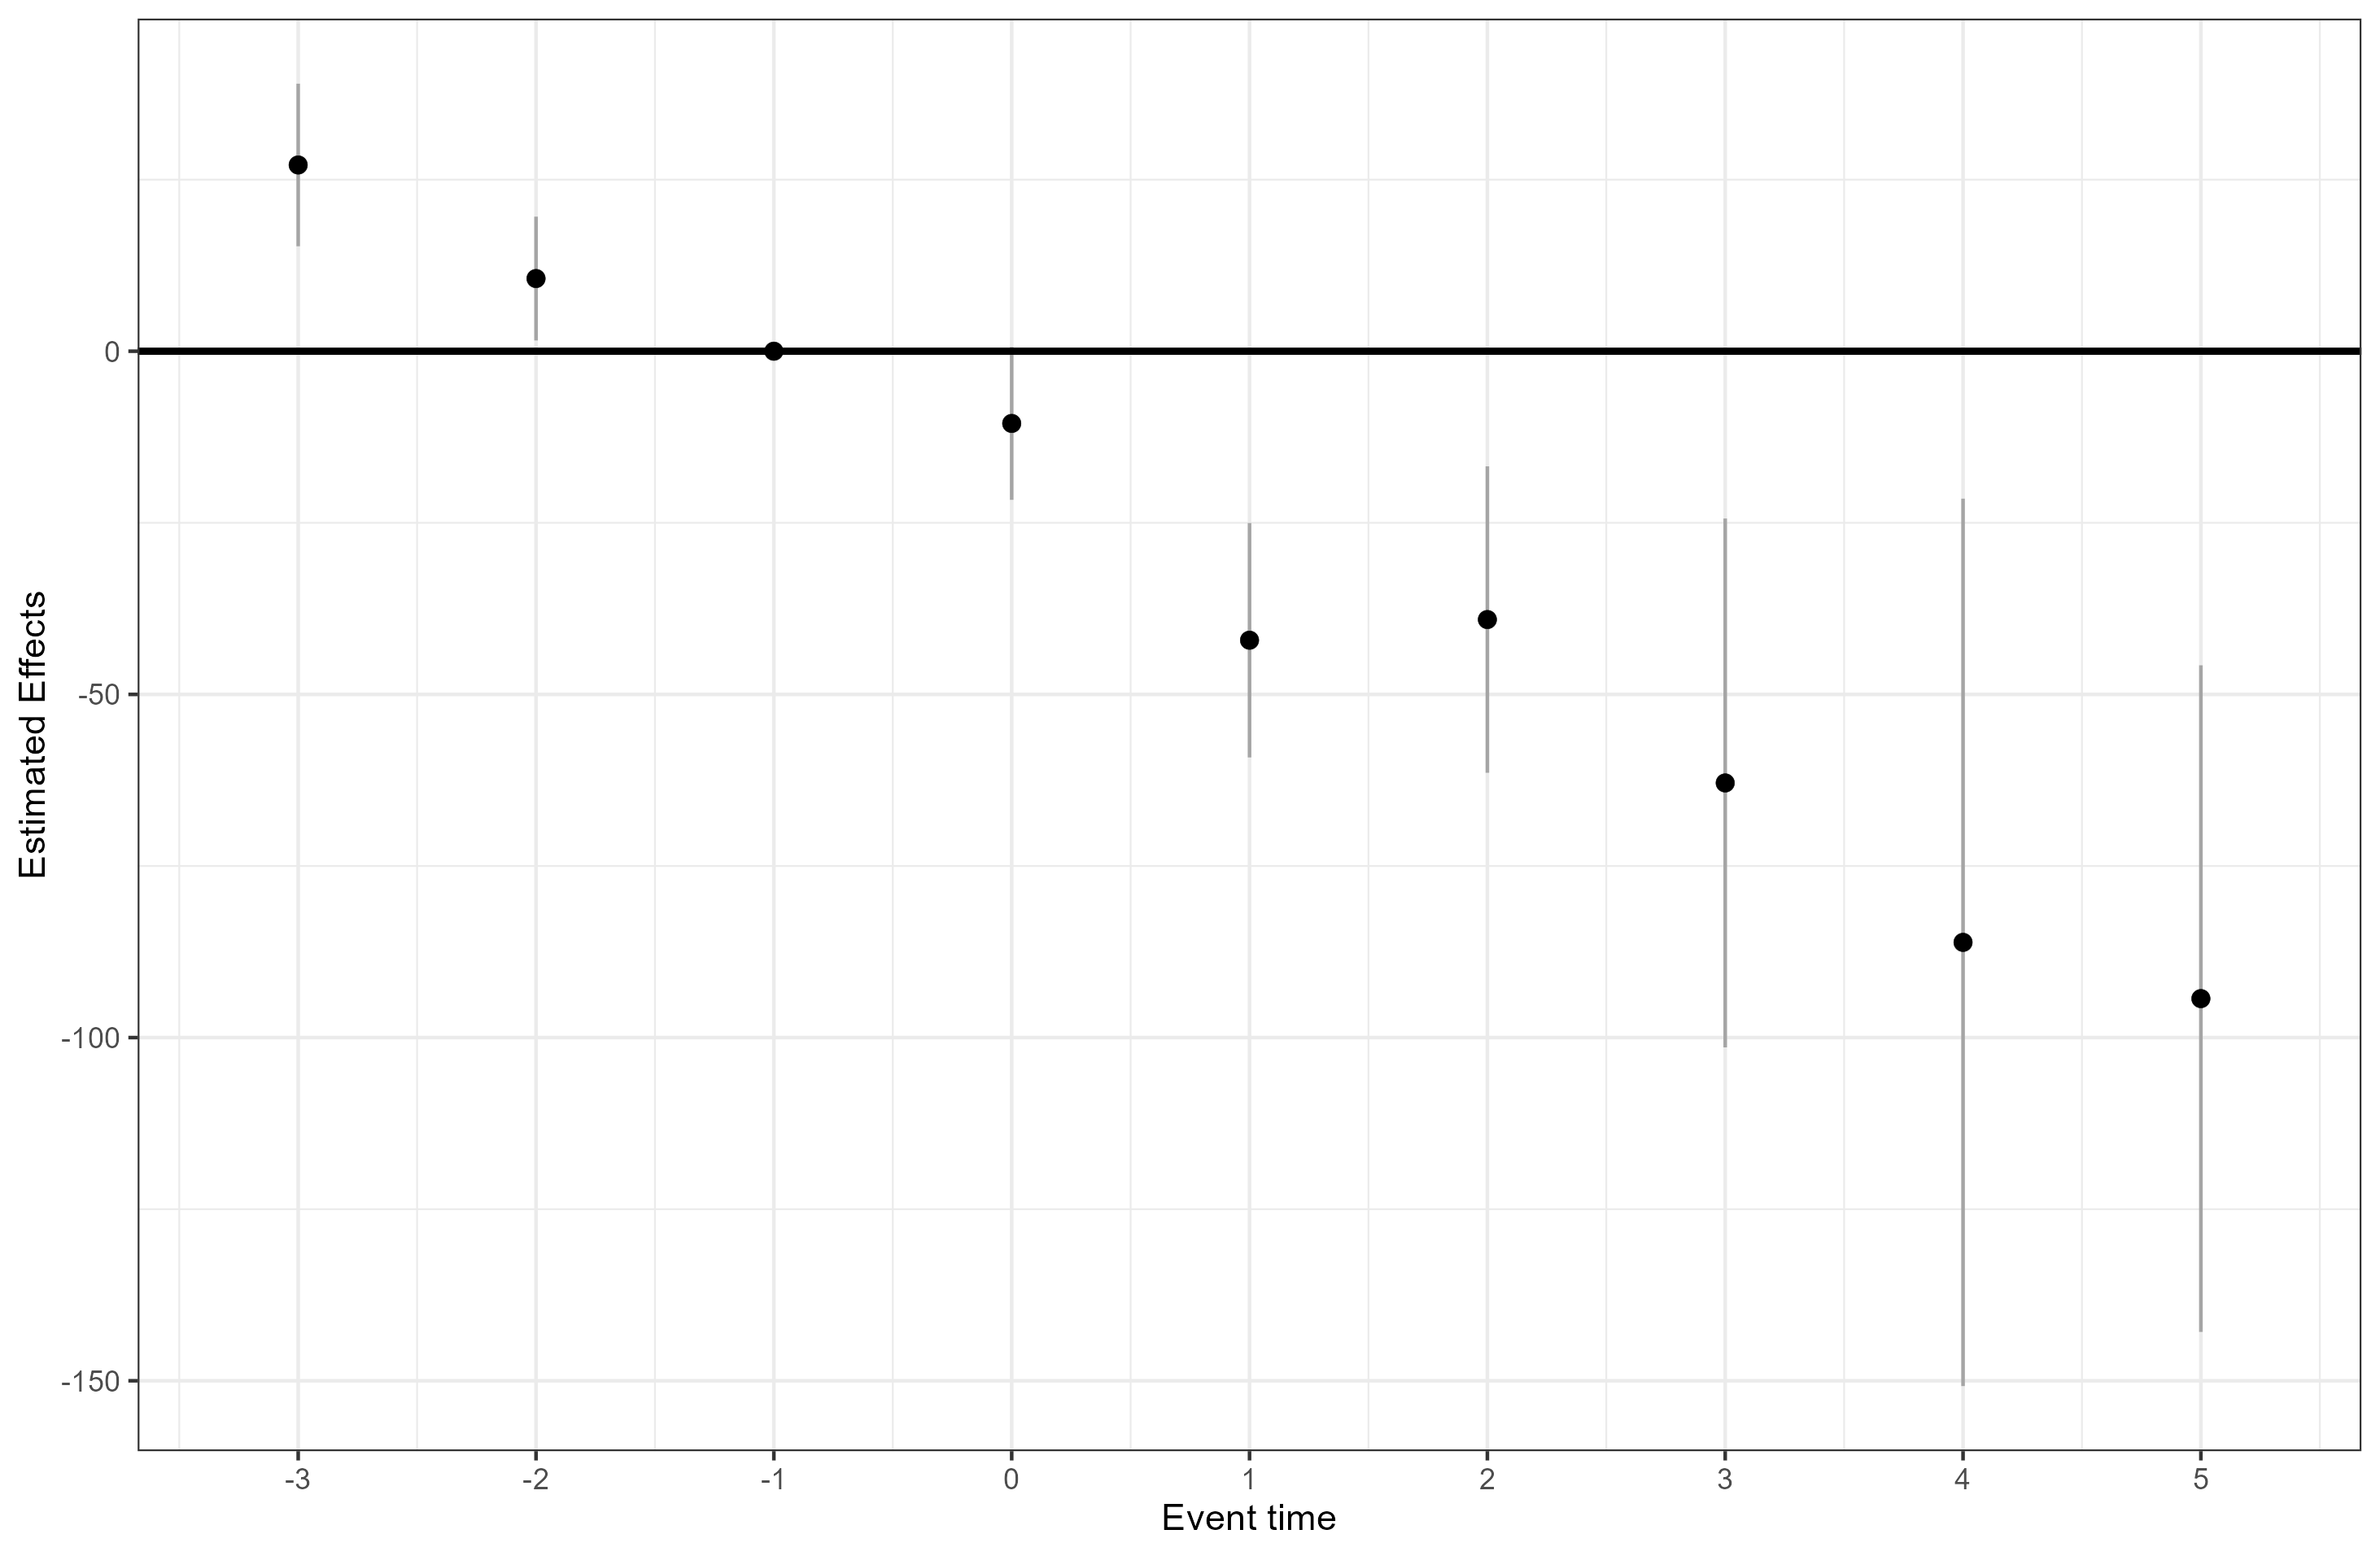
\includegraphics[width=0.48\textwidth]{../results/totopexp-cs.png} \\
\small (c) Net Patient Revenue per Bed & \small (d) Operating Expenses per Bed \\[0.5cm]
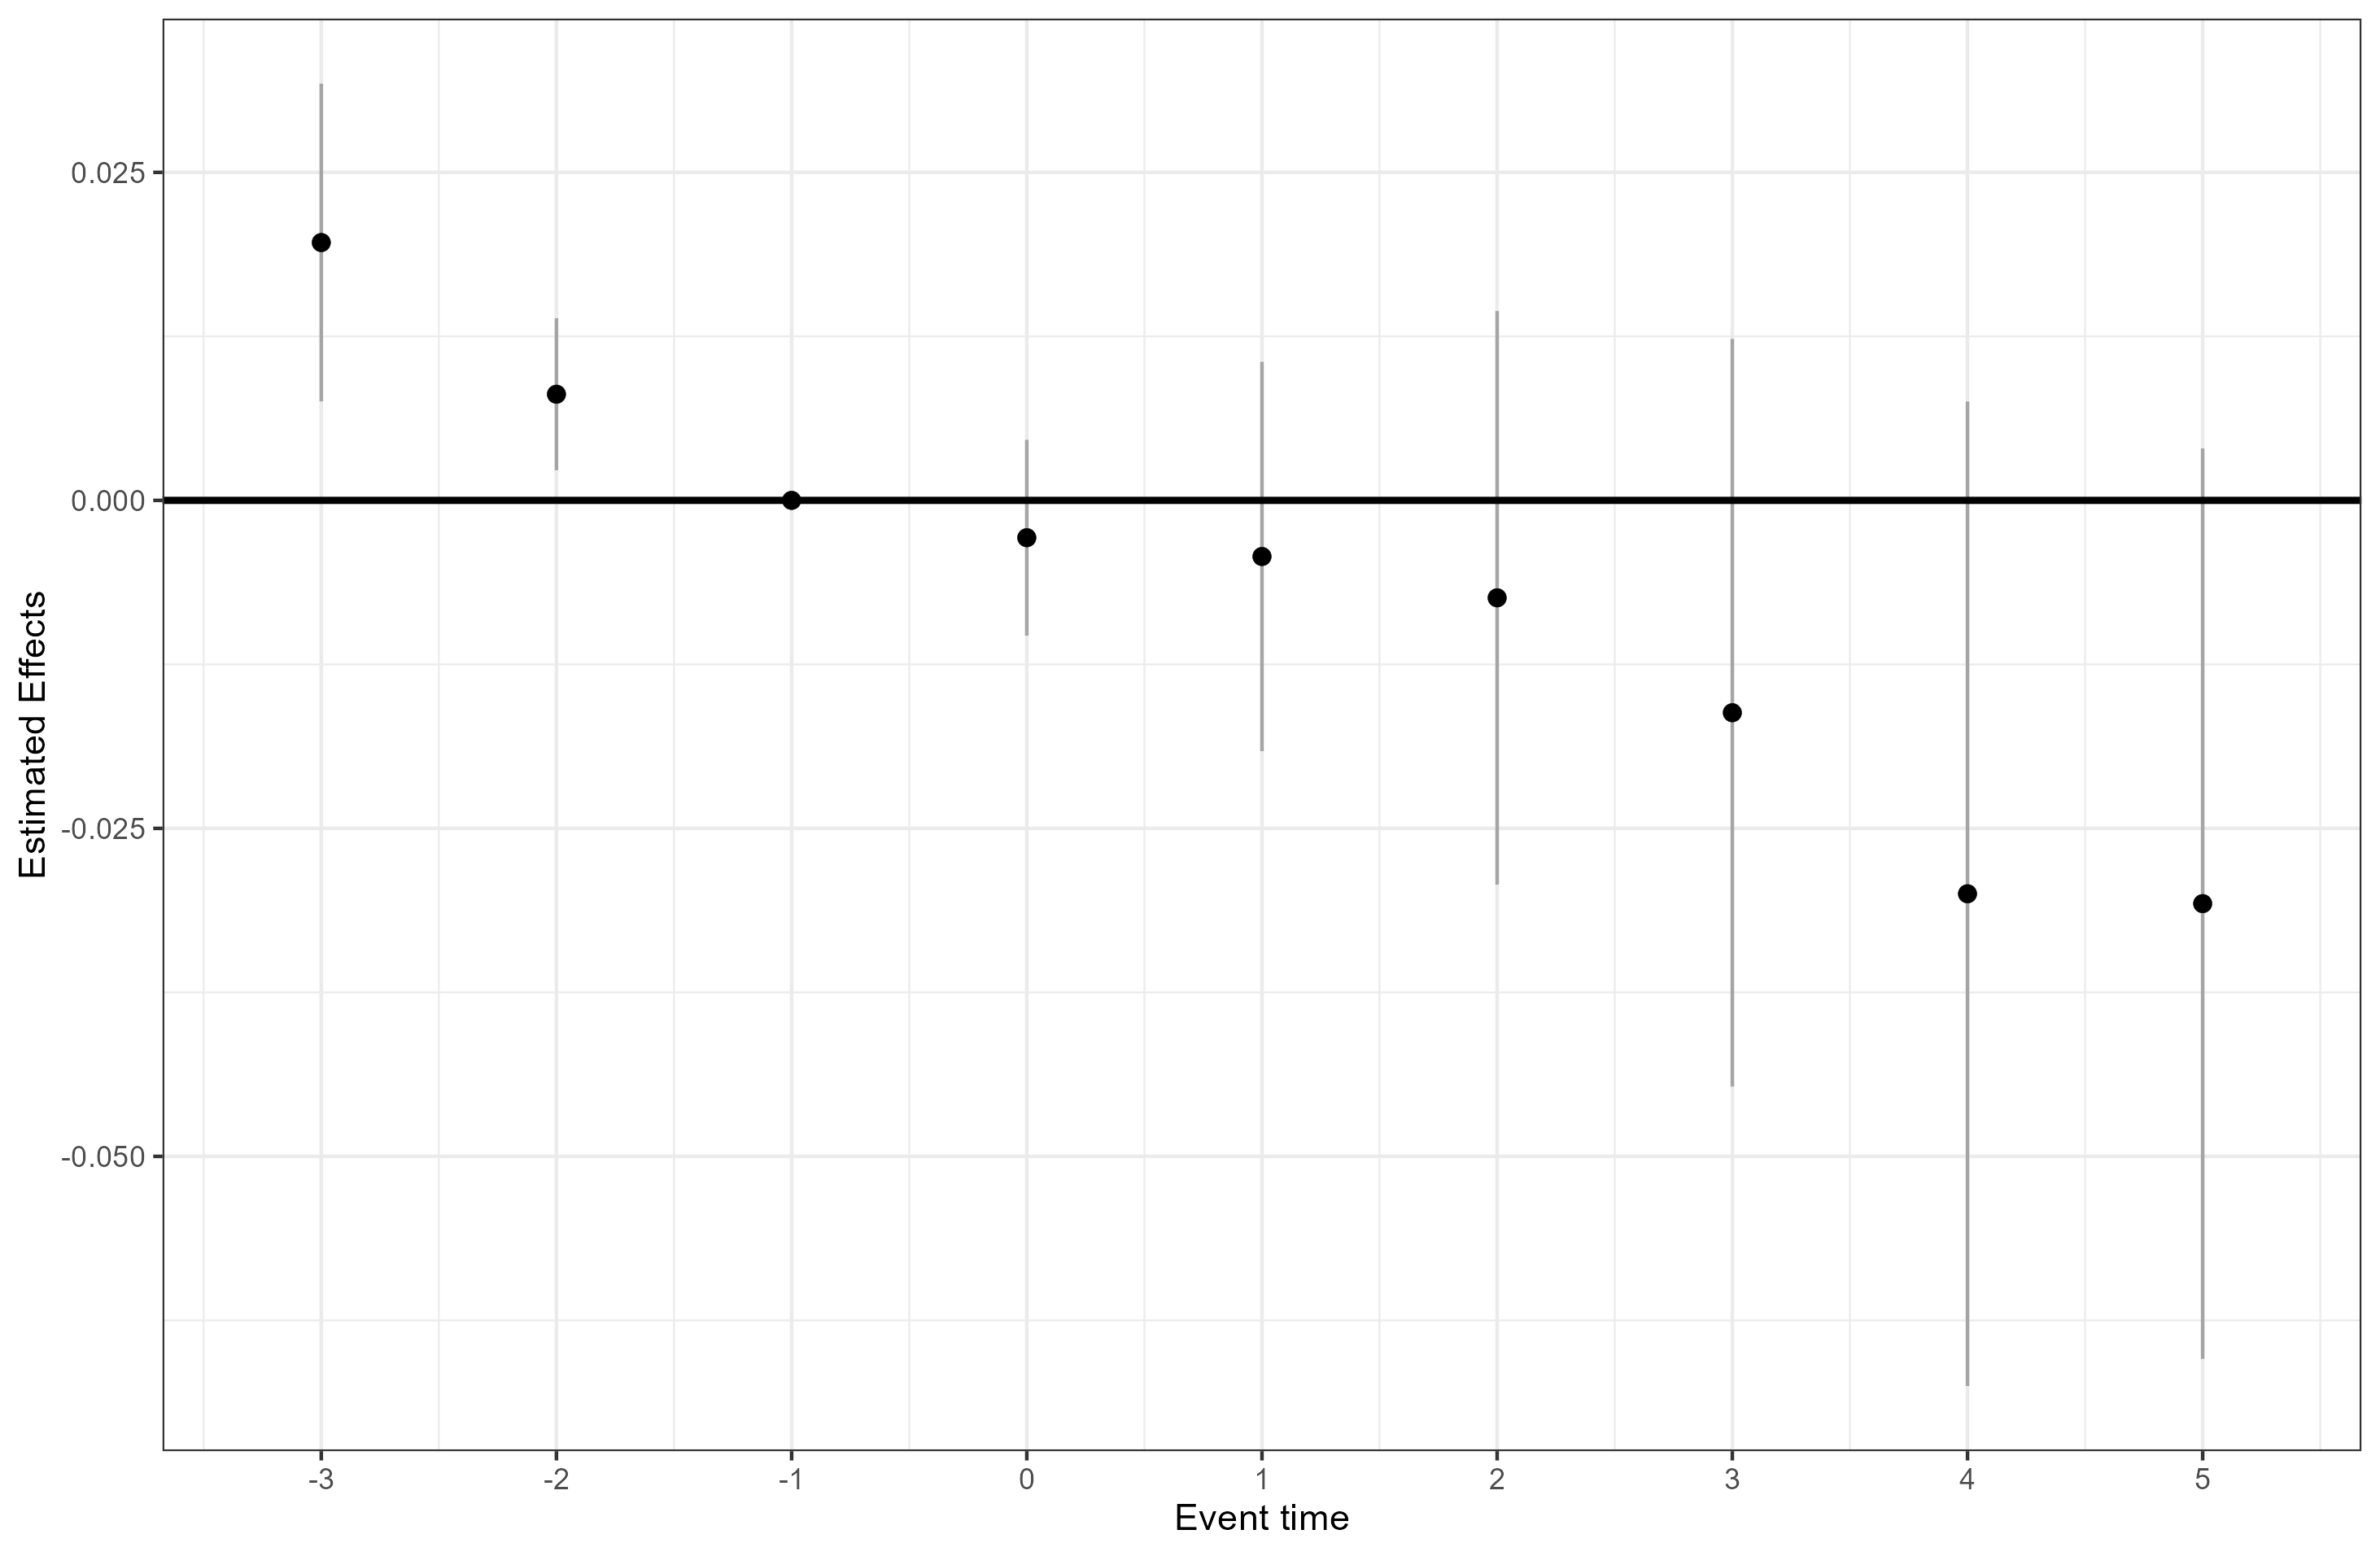
\includegraphics[width=0.48\textwidth]{../results/netfixed-cs.png} &
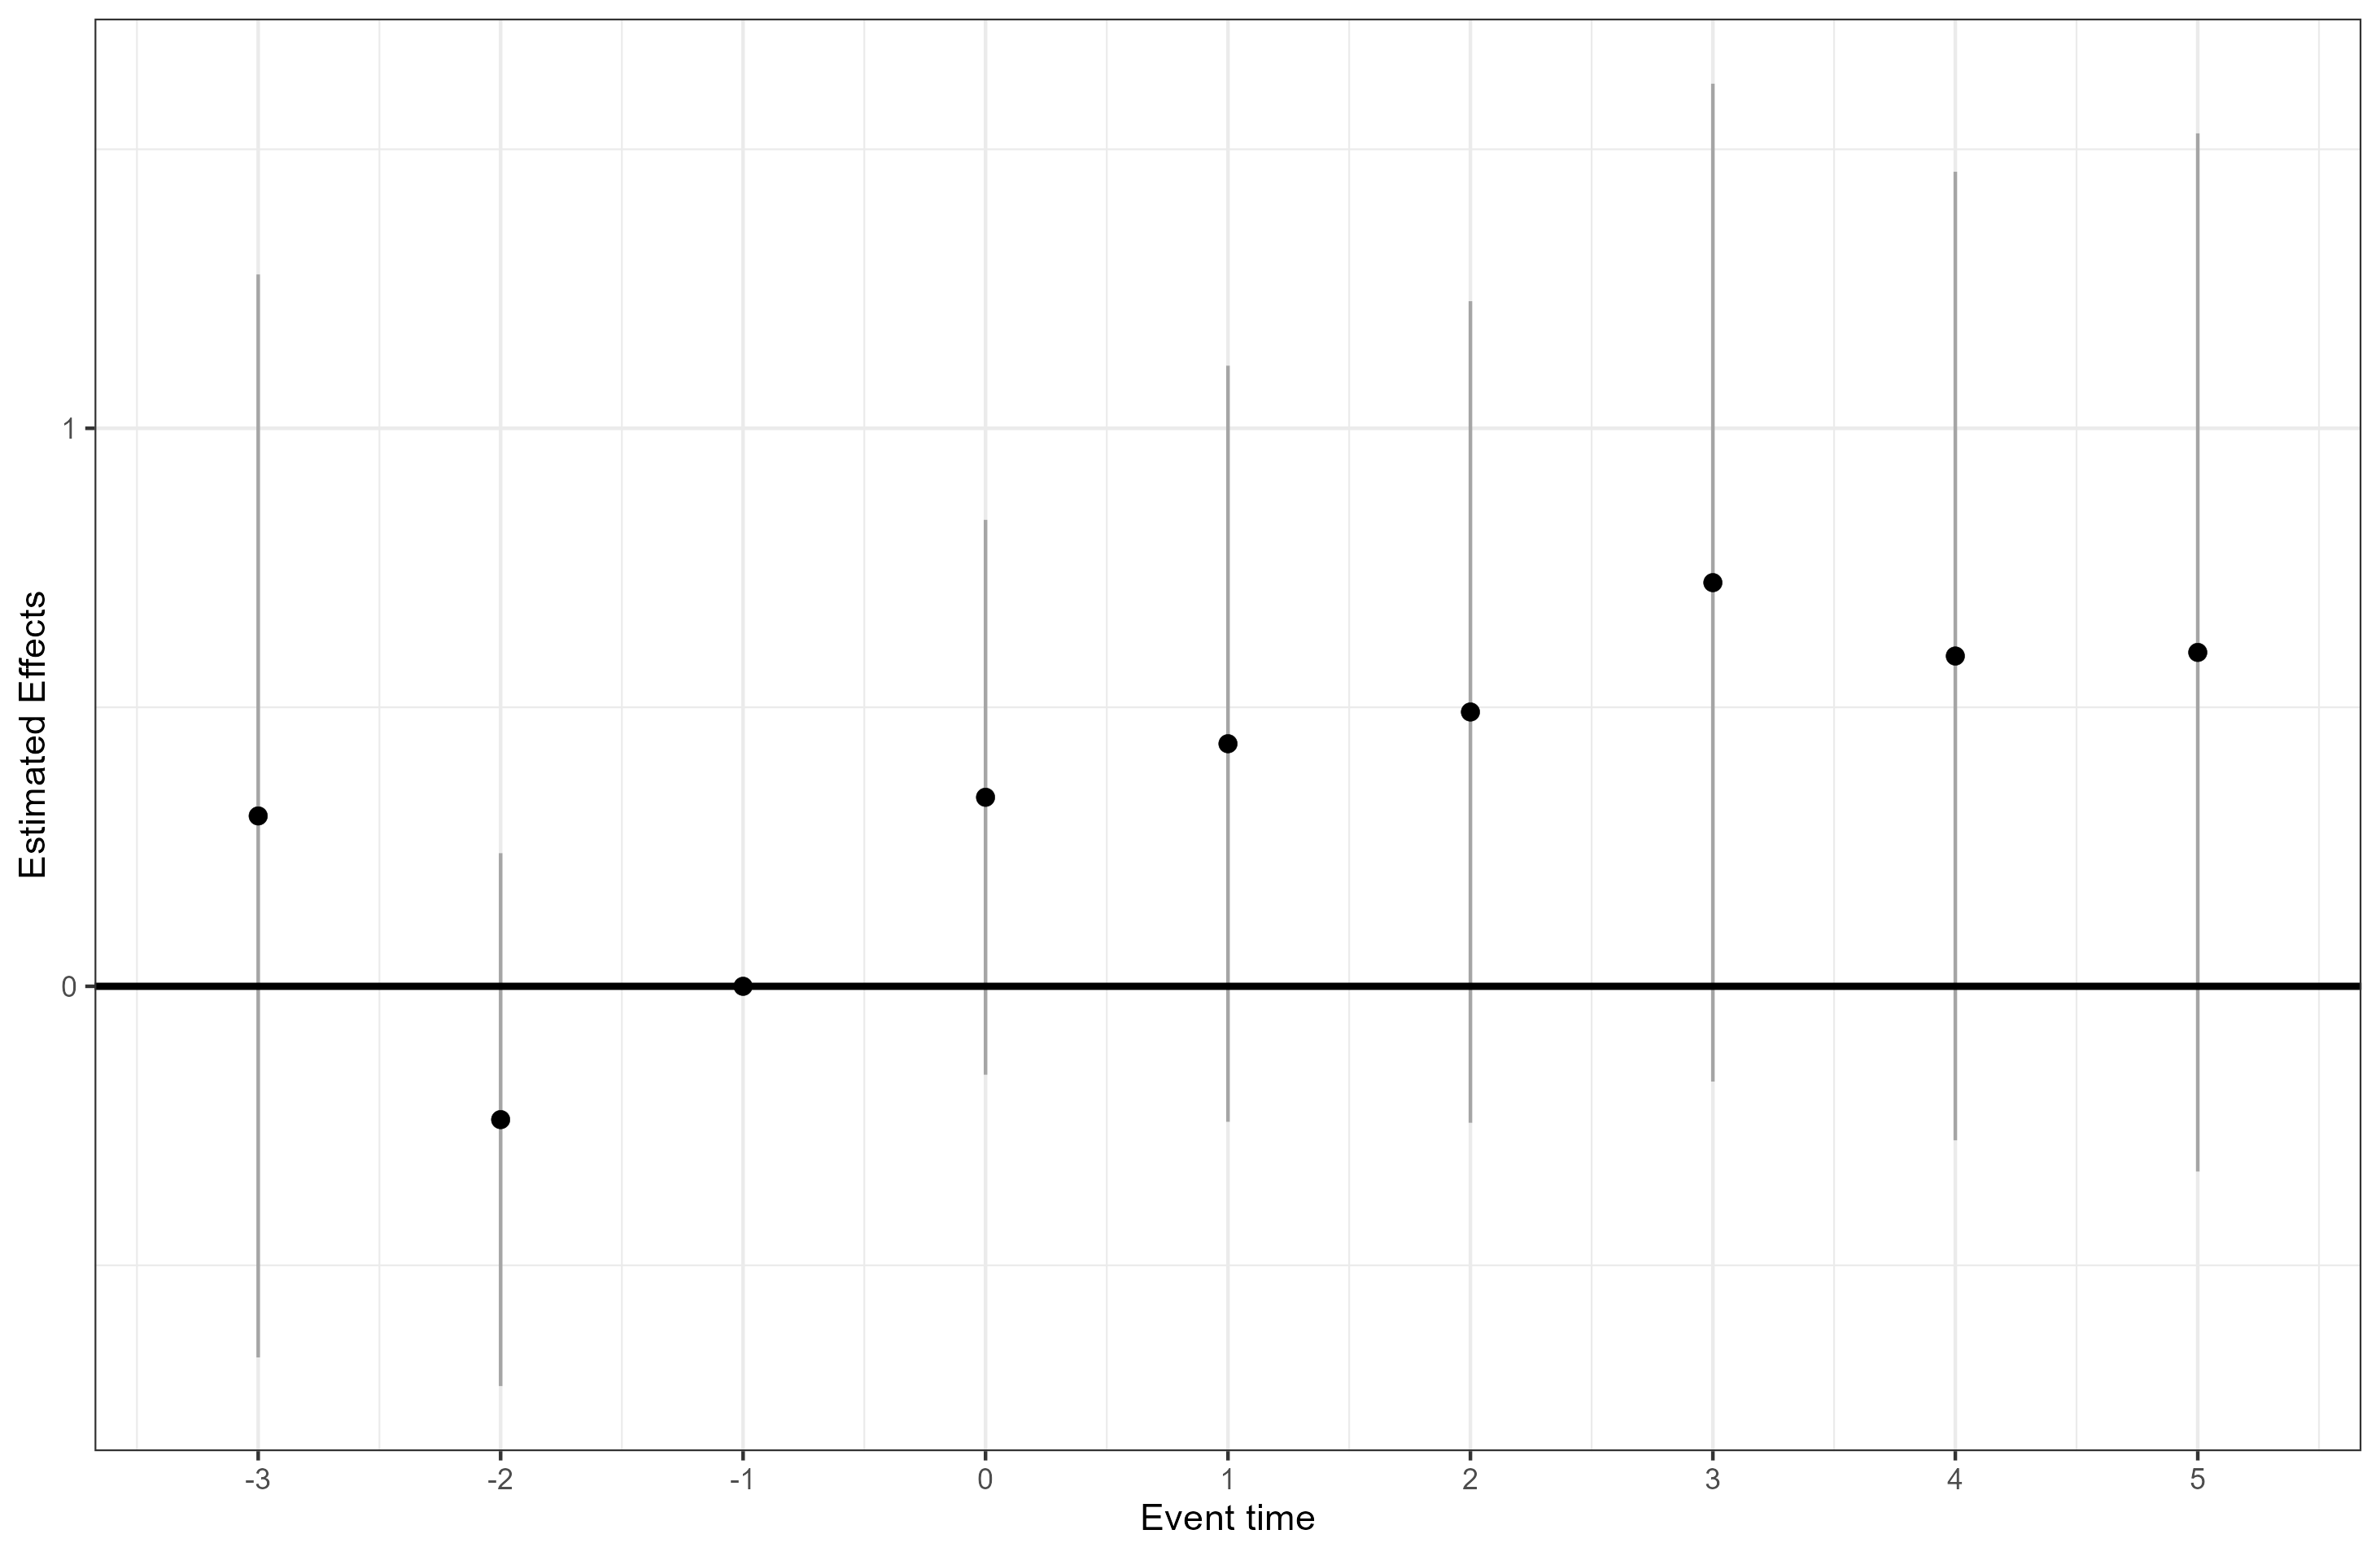
\includegraphics[width=0.48\textwidth]{../results/capex-cs.png} \\
\small (e) Net Fixed Assets & \small (f) Capital Expenditures
\end{tabular}
\end{minipage}
\end{figure}

\clearpage

\begin{figure}[!h]
\centering
\begin{minipage}[h]{6in}
\caption[CS Event Studies: Capacity]{\textbf{CS Event-Study Estimates: Capacity and Staffing}\footnote{Callaway--Sant'Anna event-study estimates with 95\% confidence intervals by years relative to designation, state-timing design (cohorts 1999--2001), not-yet-treated control group, universal base period.}}
\label{fig:cs-capacity}
\begin{tabular}{cc}
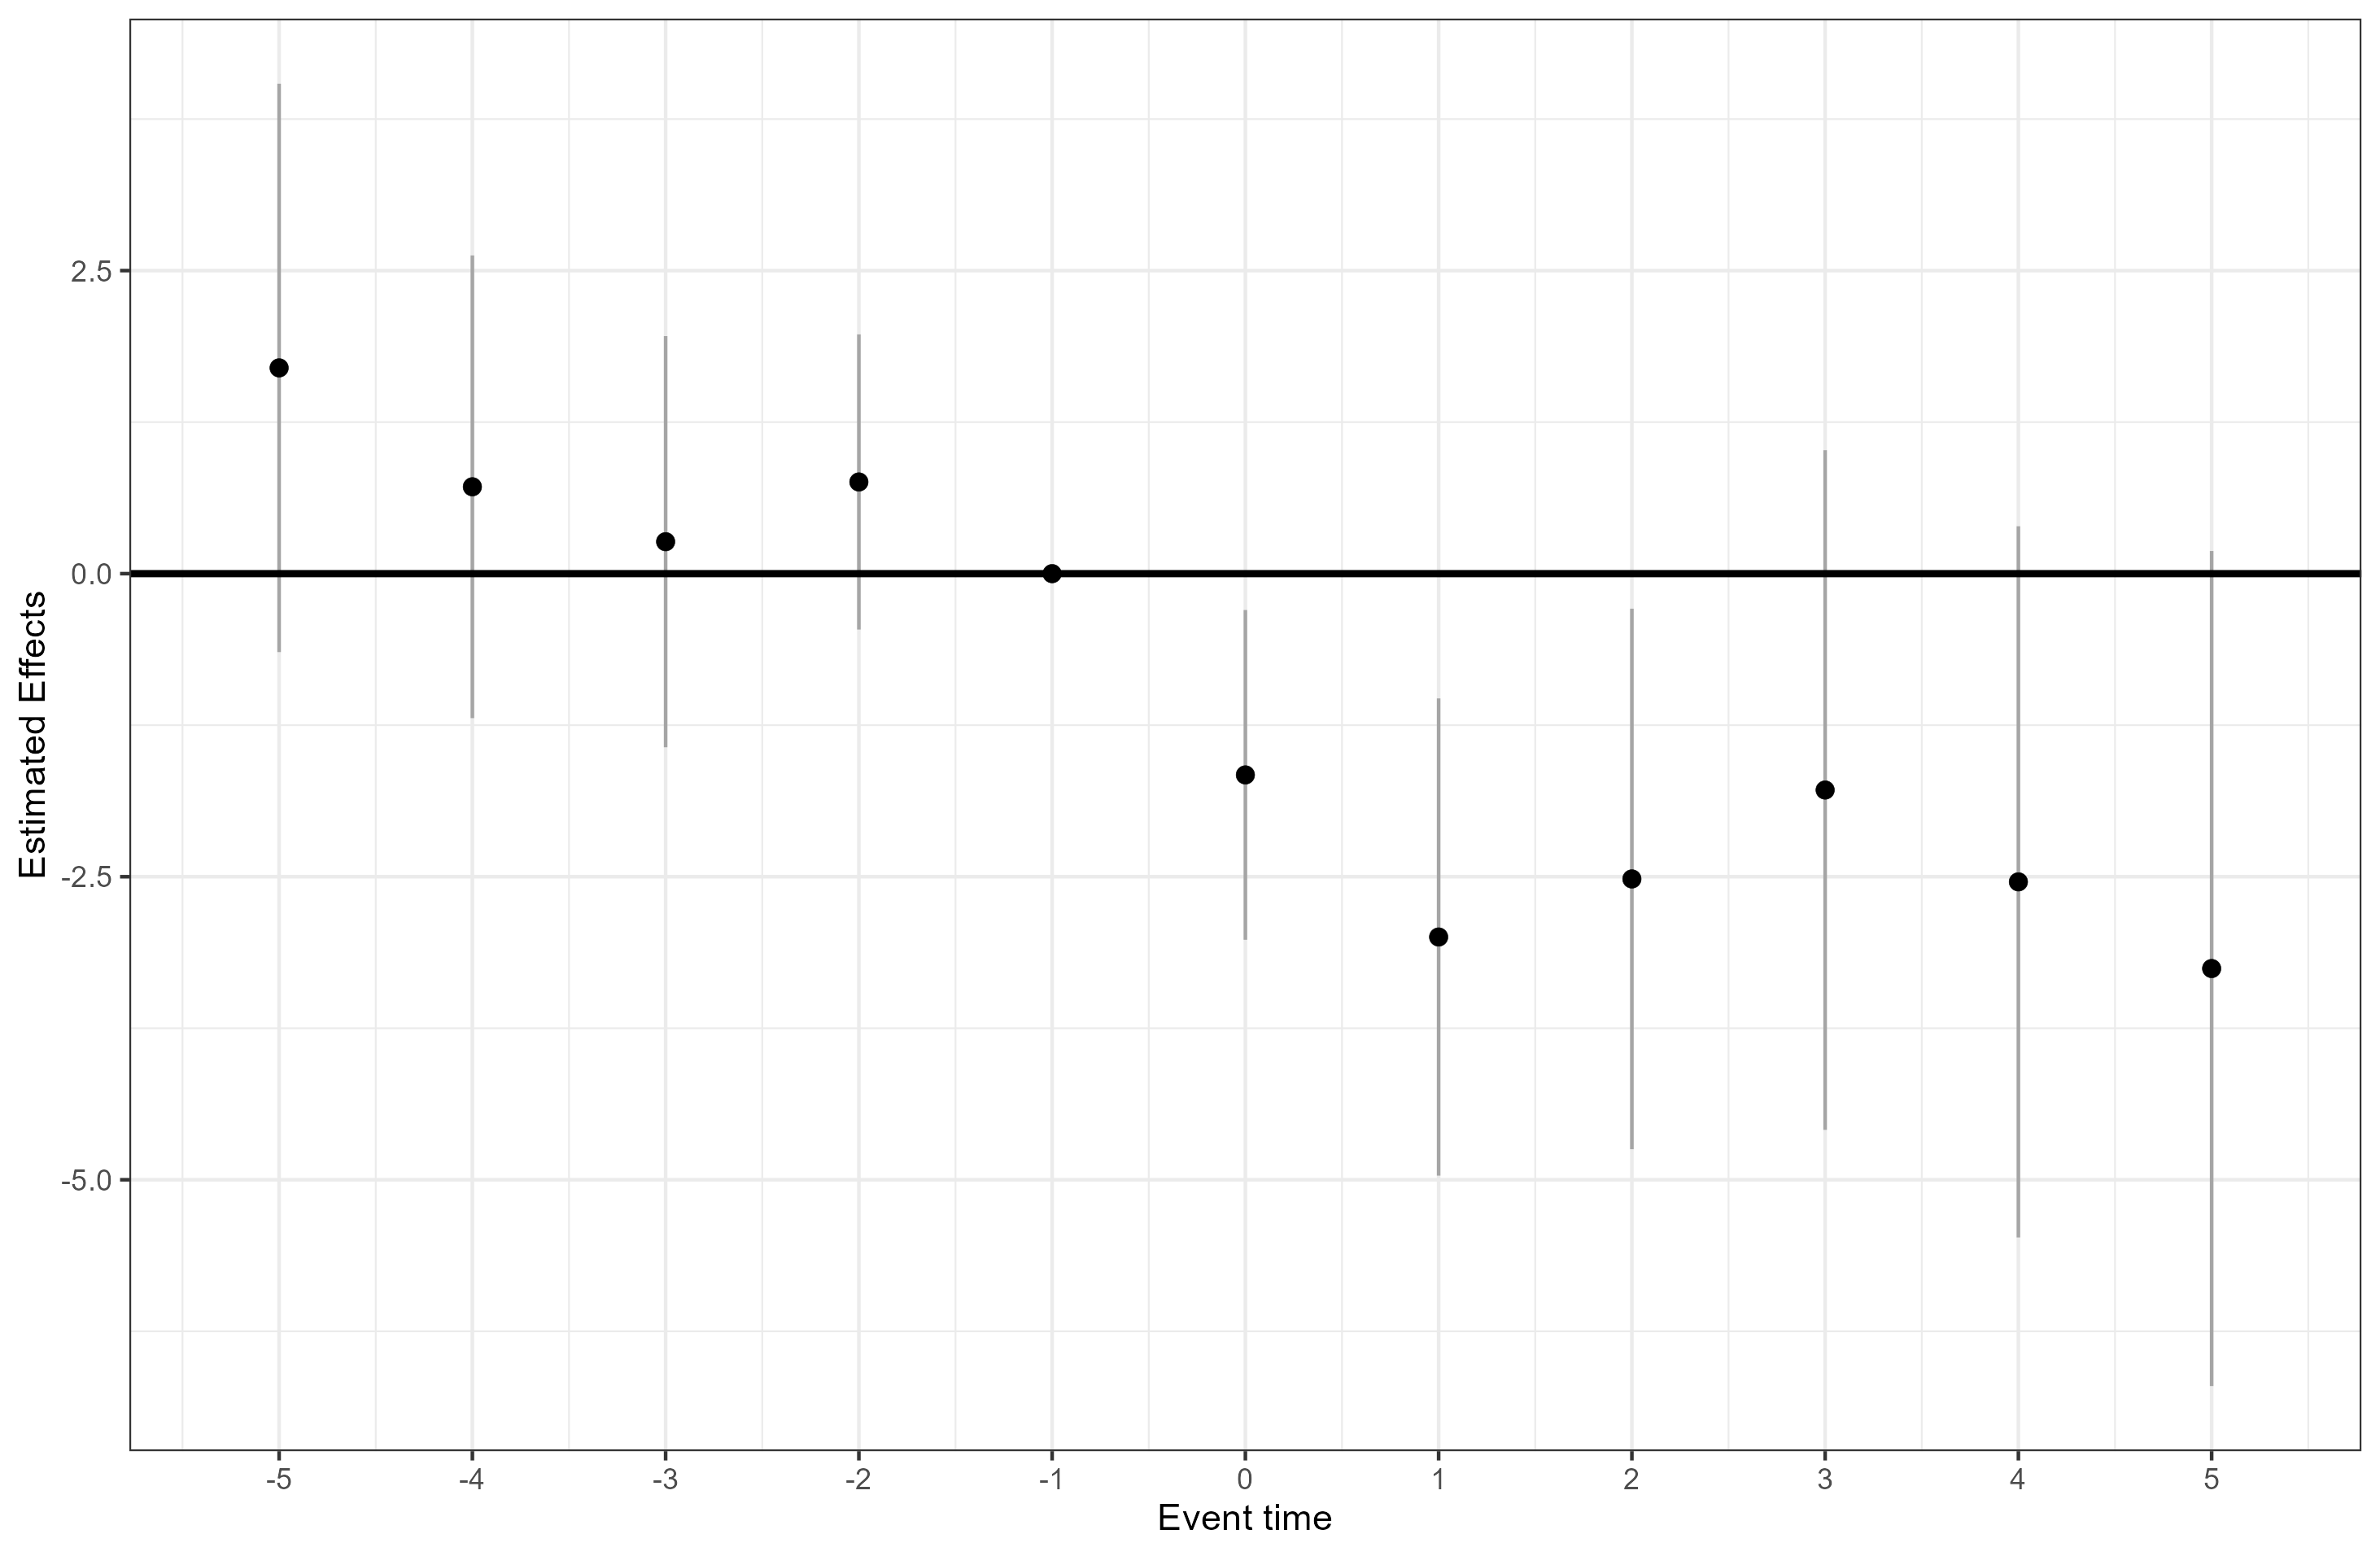
\includegraphics[width=0.48\textwidth]{../results/beds-cs.png} &
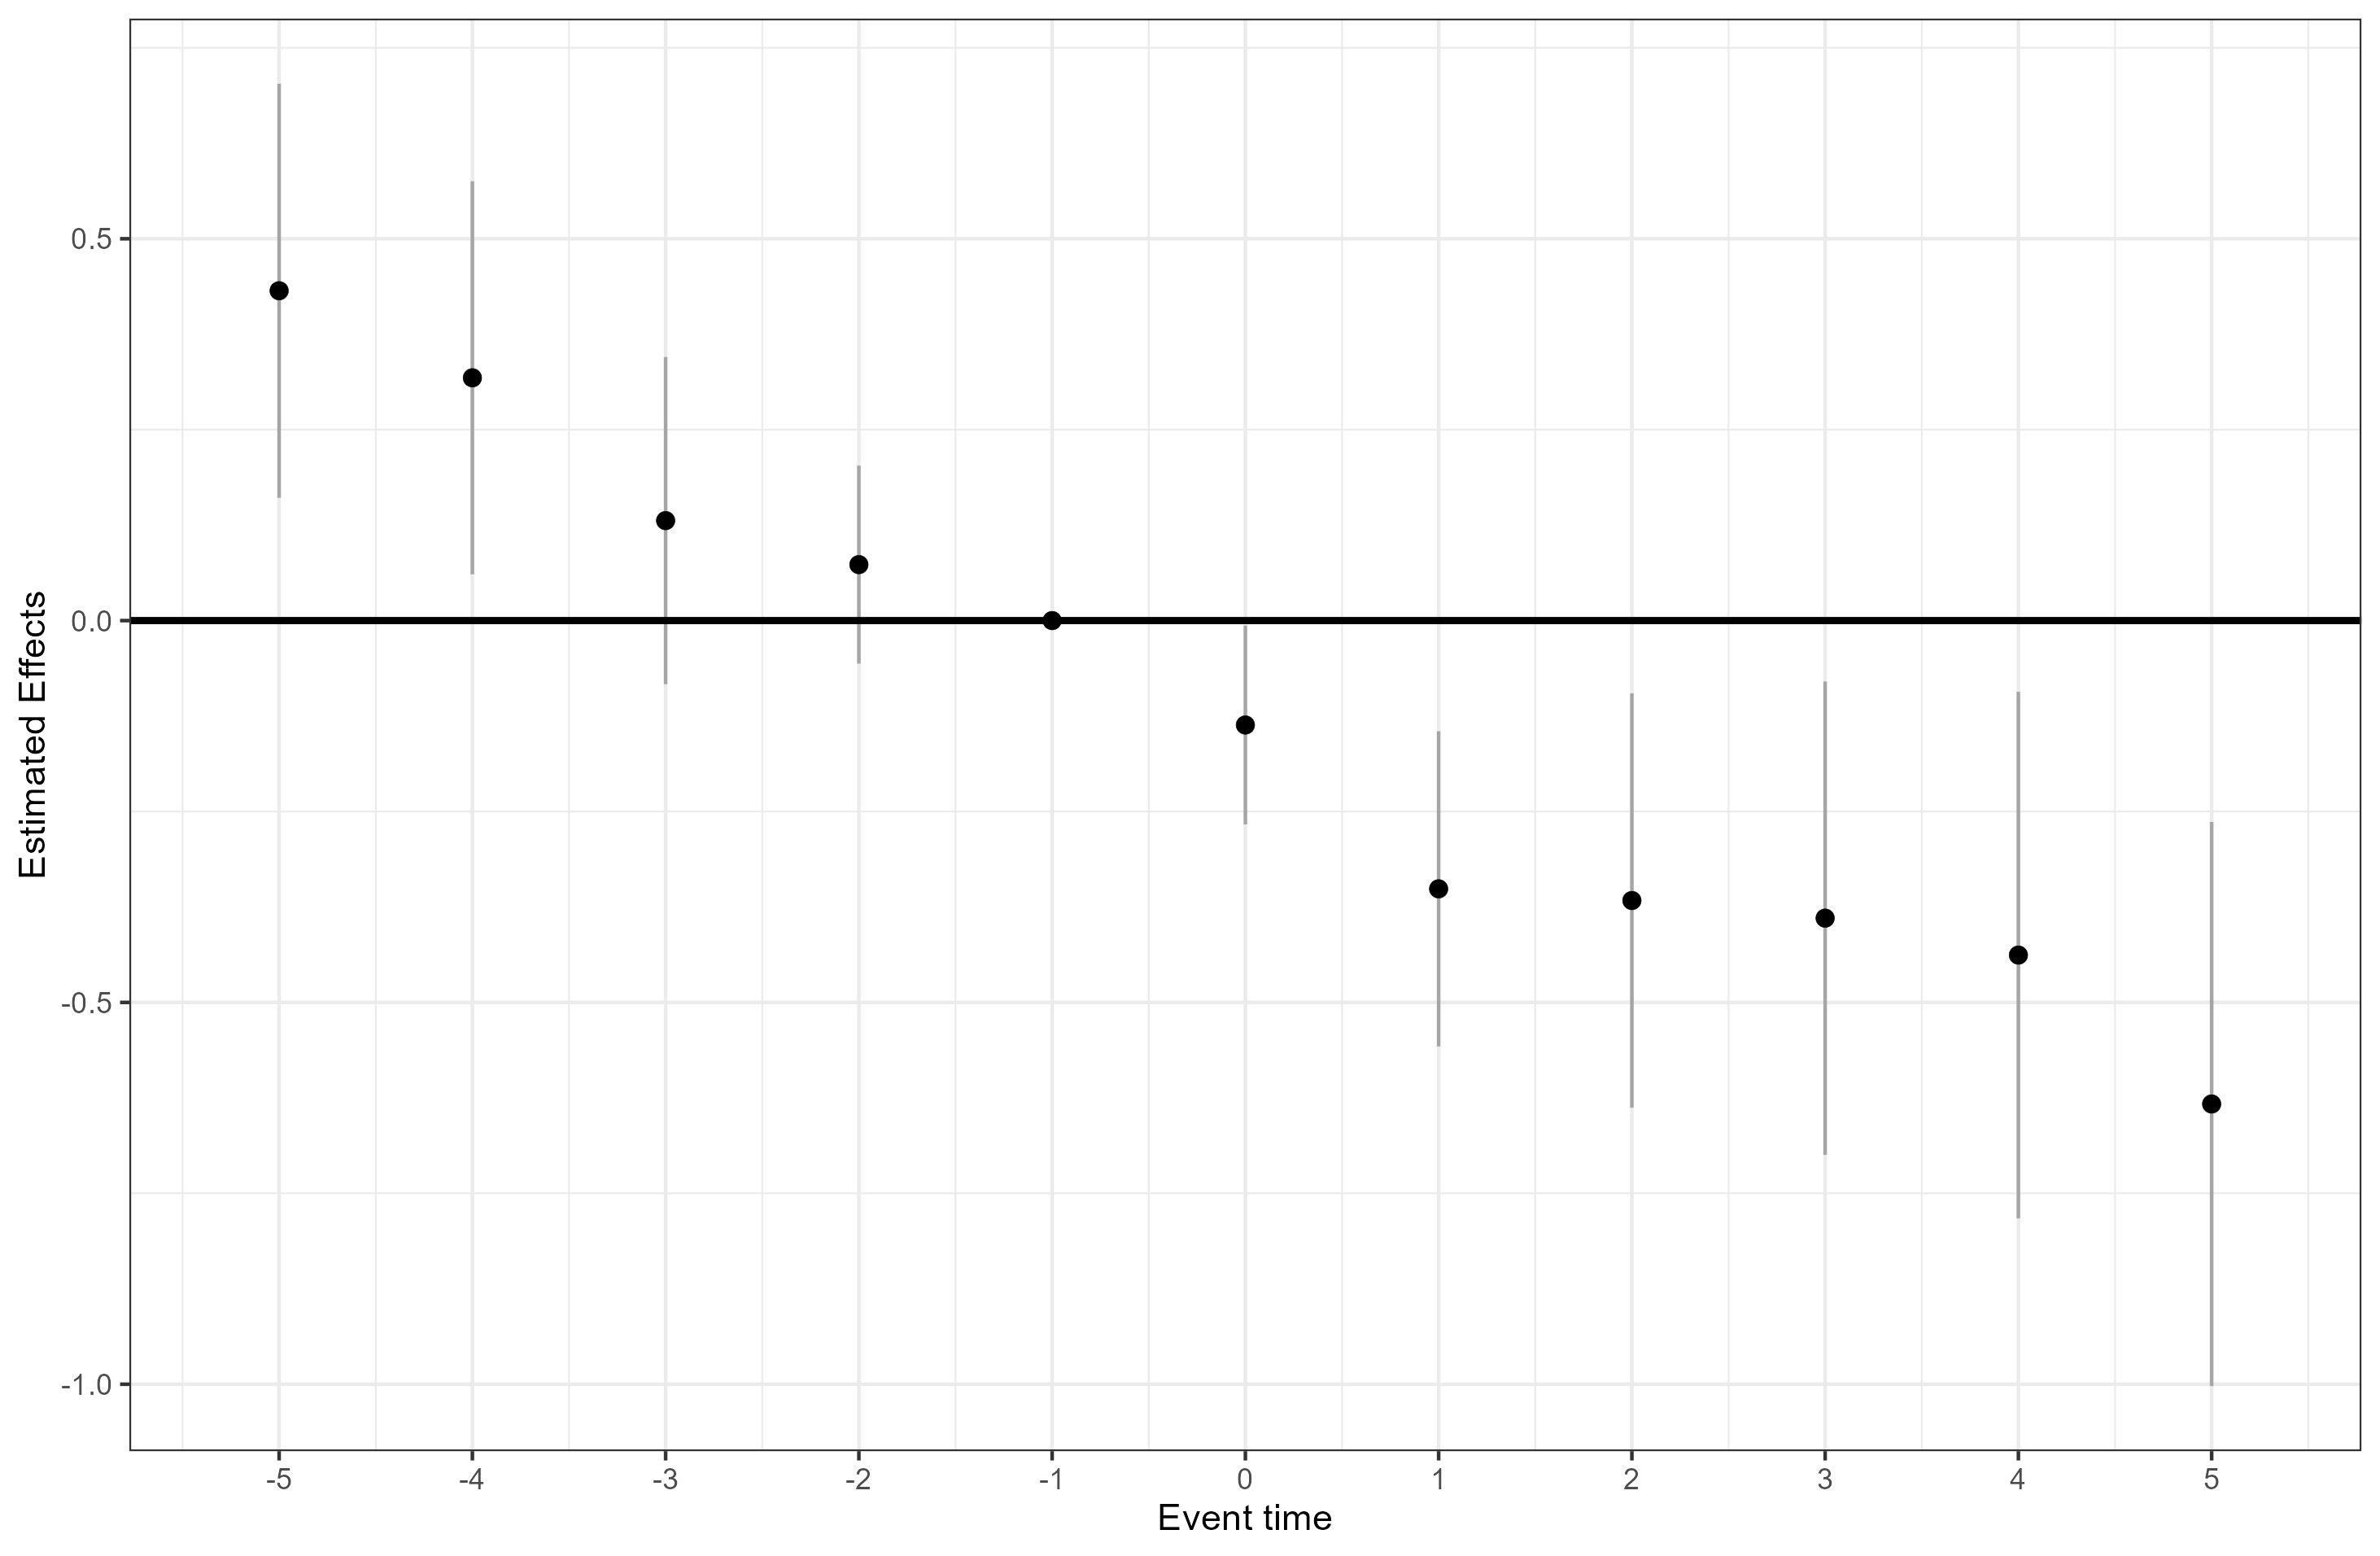
\includegraphics[width=0.48\textwidth]{../results/beds_ob-cs.png} \\
\small (a) Total Beds & \small (b) Obstetric Beds \\[0.5cm]
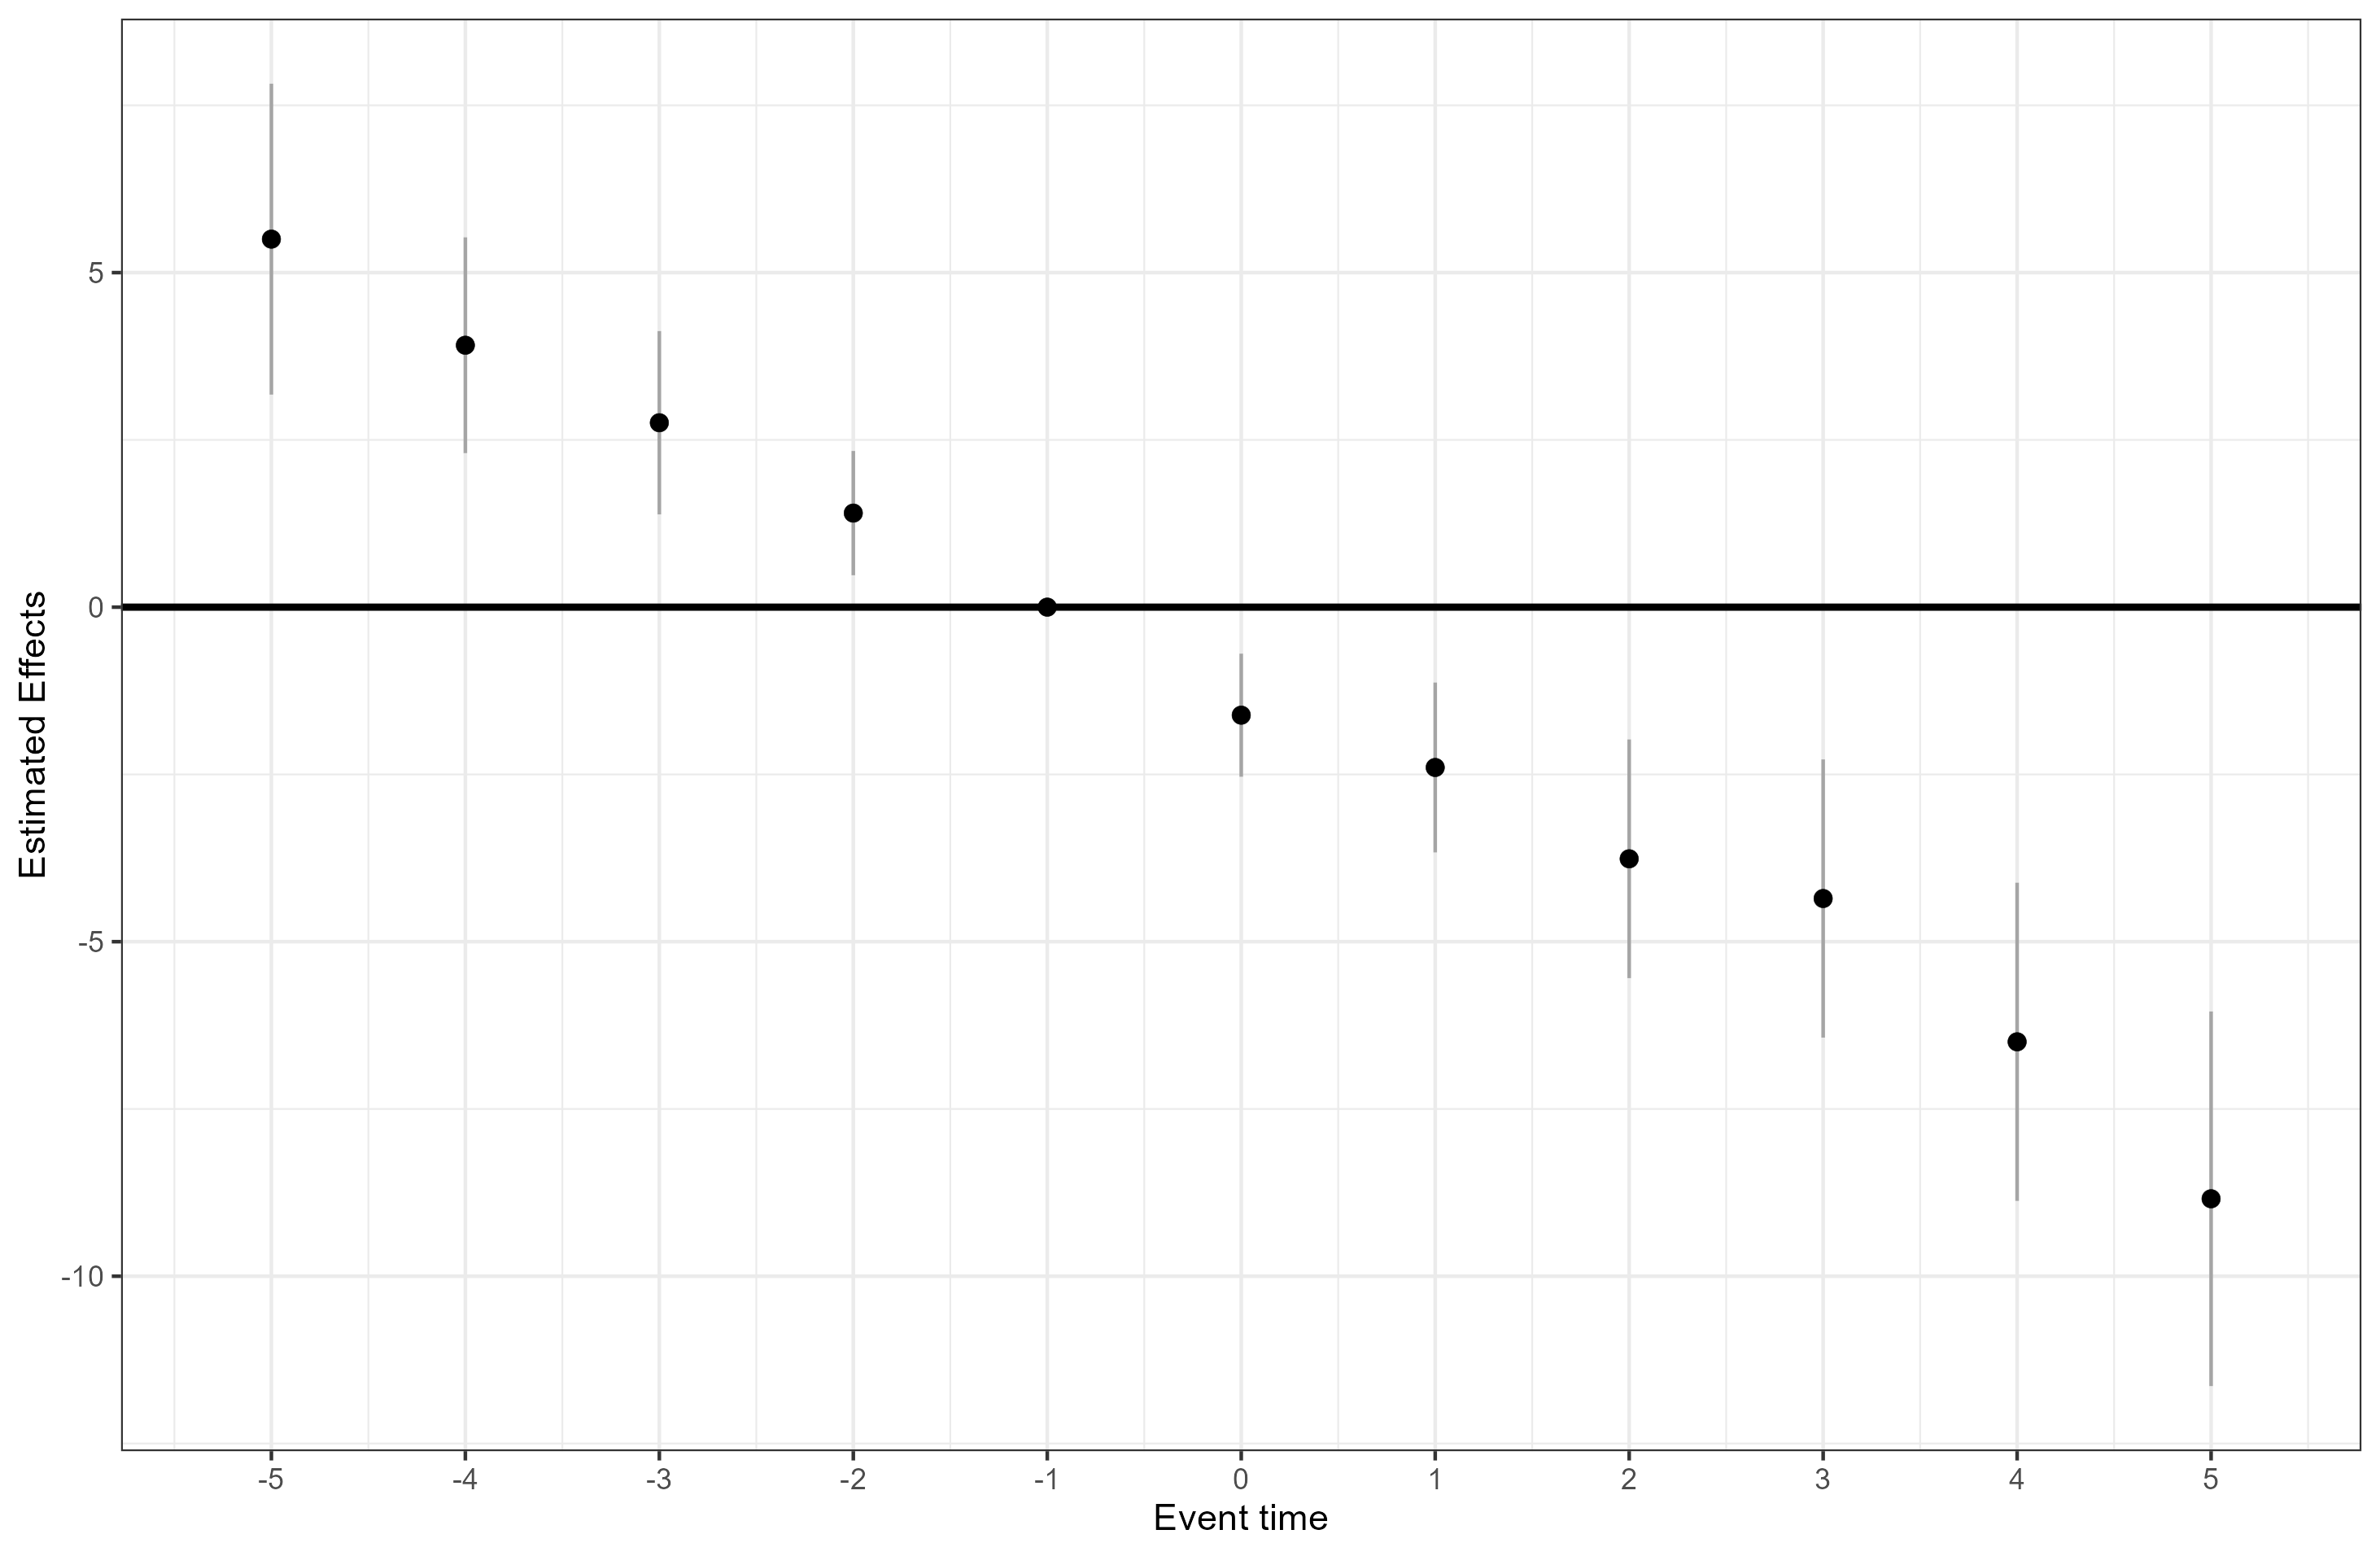
\includegraphics[width=0.48\textwidth]{../results/ftern-cs.png} &
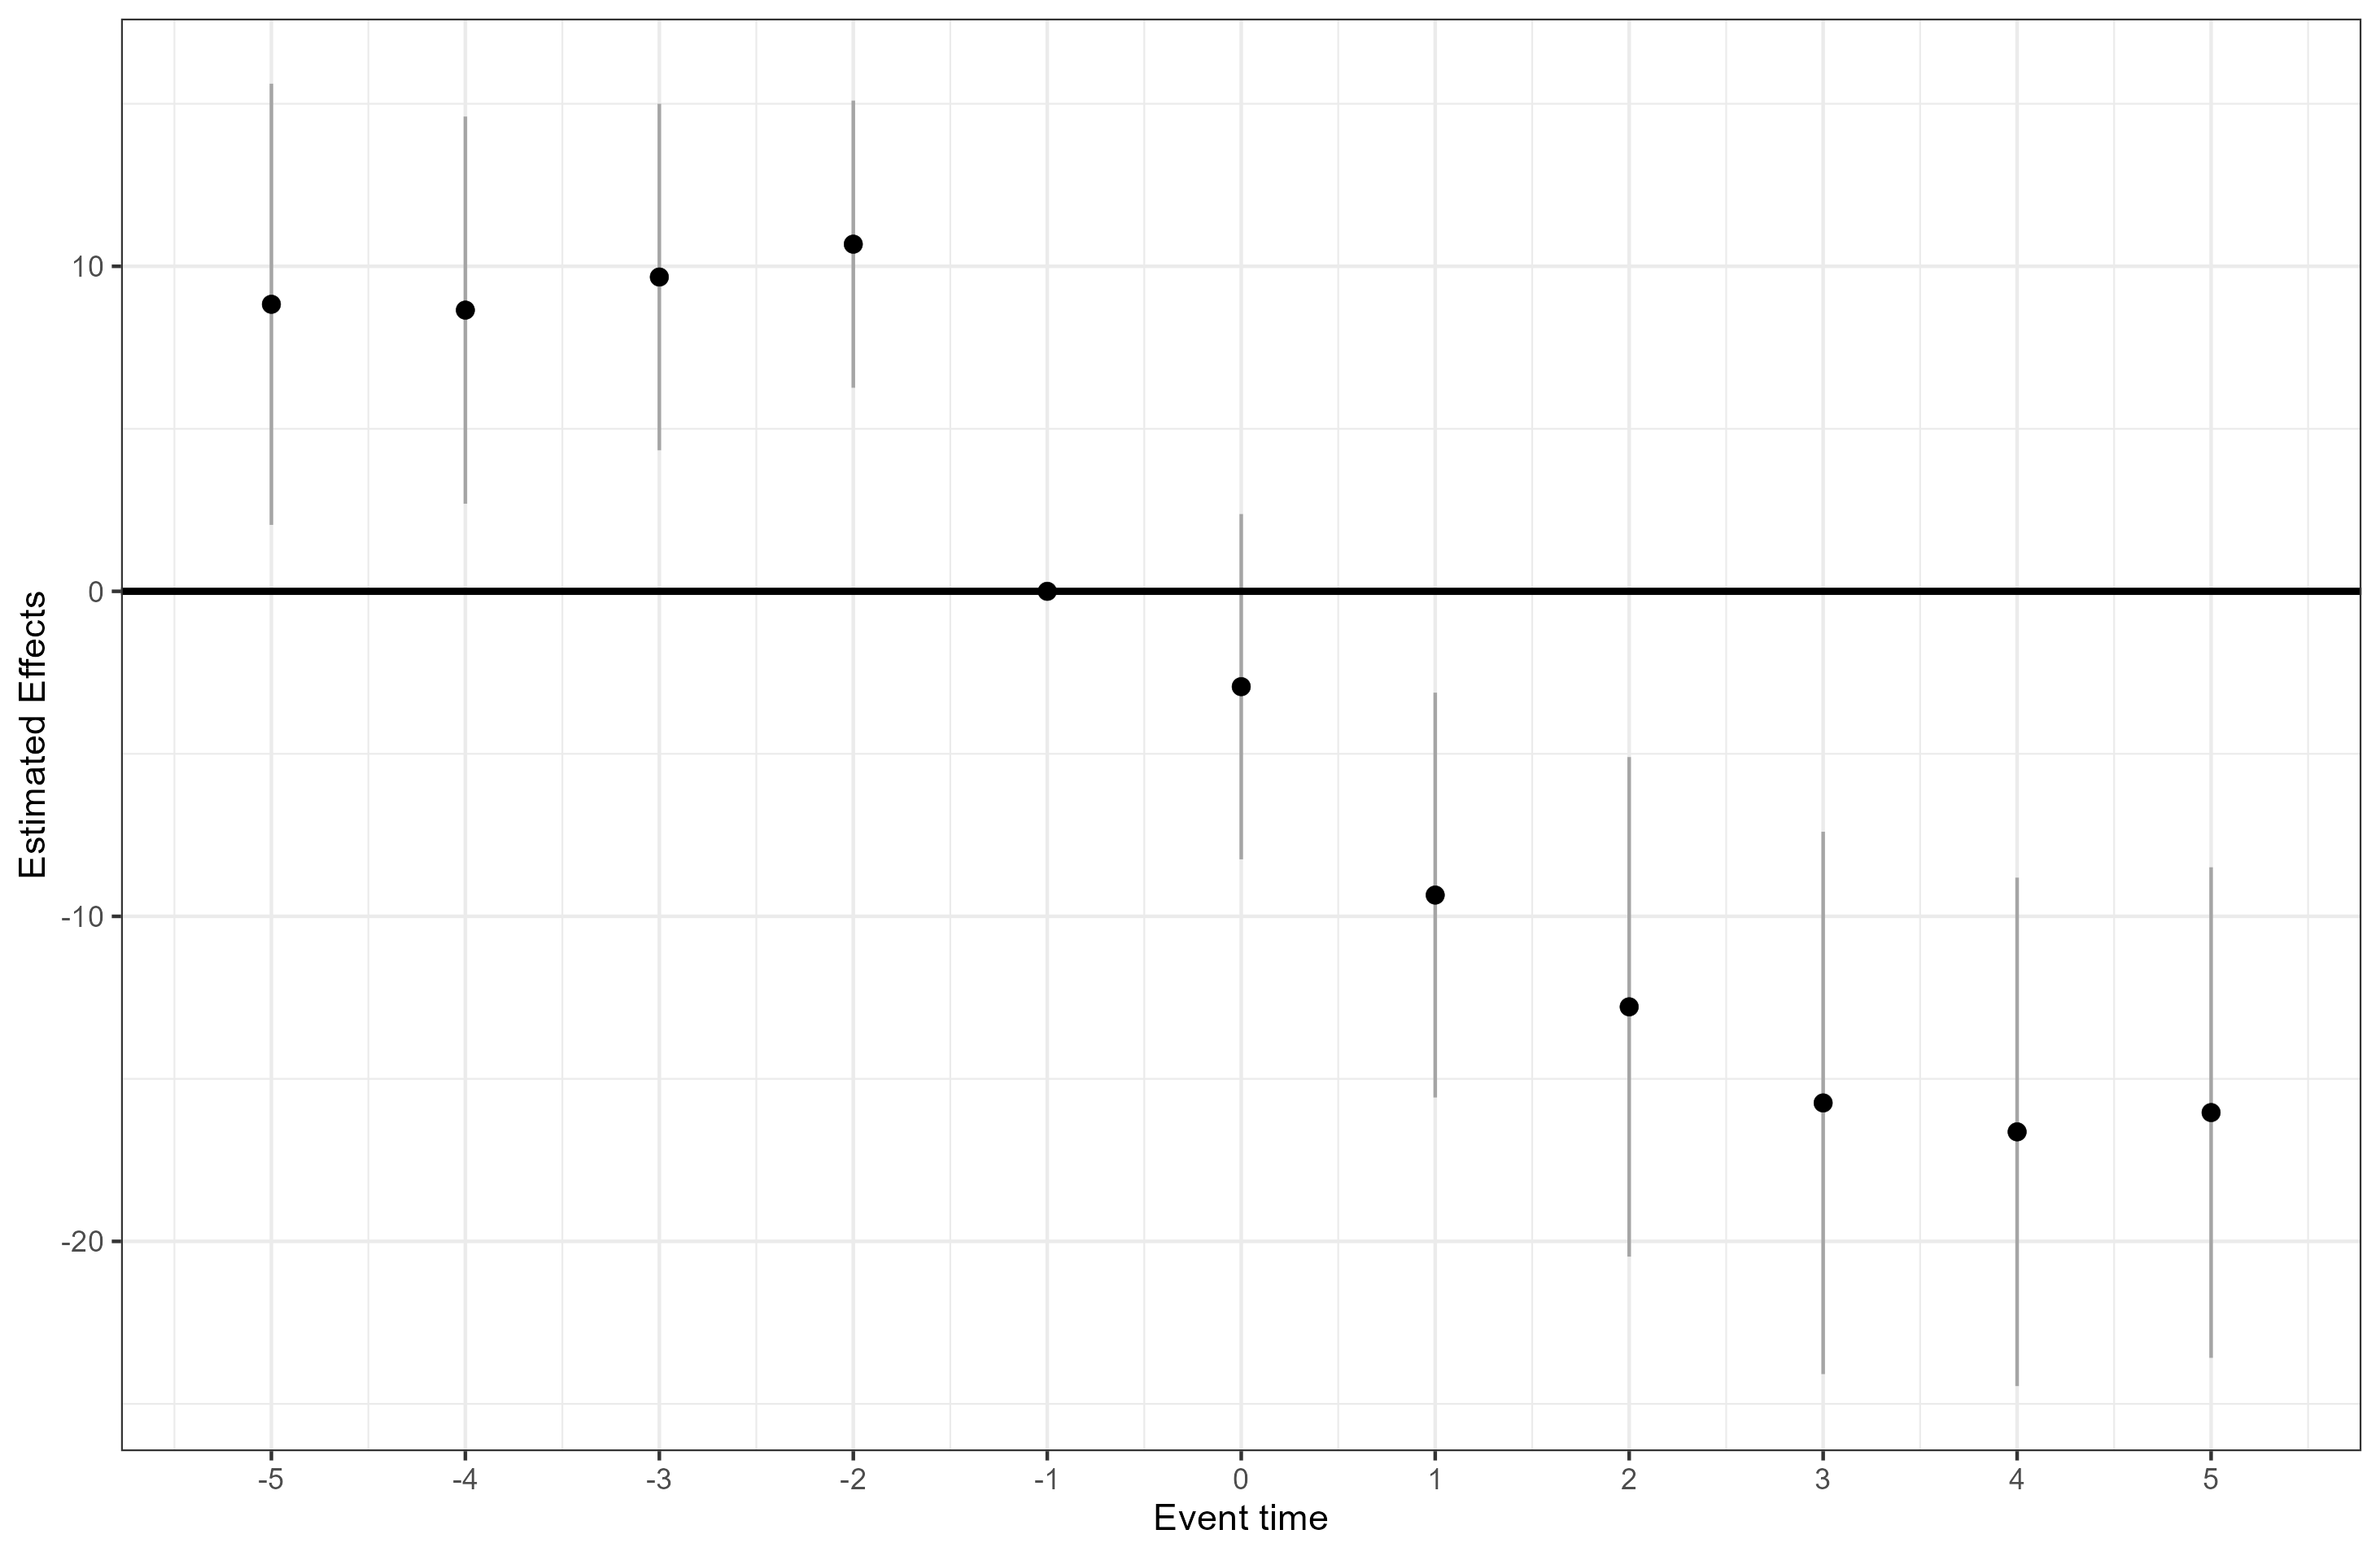
\includegraphics[width=0.48\textwidth]{../results/ipdays-cs.png} \\
\small (c) Full Time Equivalent RNs & \small (d) Inpatient Days per Bed
\end{tabular}
\end{minipage}
\end{figure}

\clearpage

\begin{figure}[!h]
\centering
\begin{minipage}[h]{6in}
\caption[CS Event Studies: Organizational]{\textbf{CS Event-Study Estimates: Organizational Changes}\footnote{Callaway--Sant'Anna event-study estimates with 95\% confidence intervals by years relative to designation, state-timing design (cohorts 1999--2001), not-yet-treated control group, universal base period. Closures and mergers are state-level counts per 100 hospitals.}}
\label{fig:cs-org}
\begin{tabular}{cc}
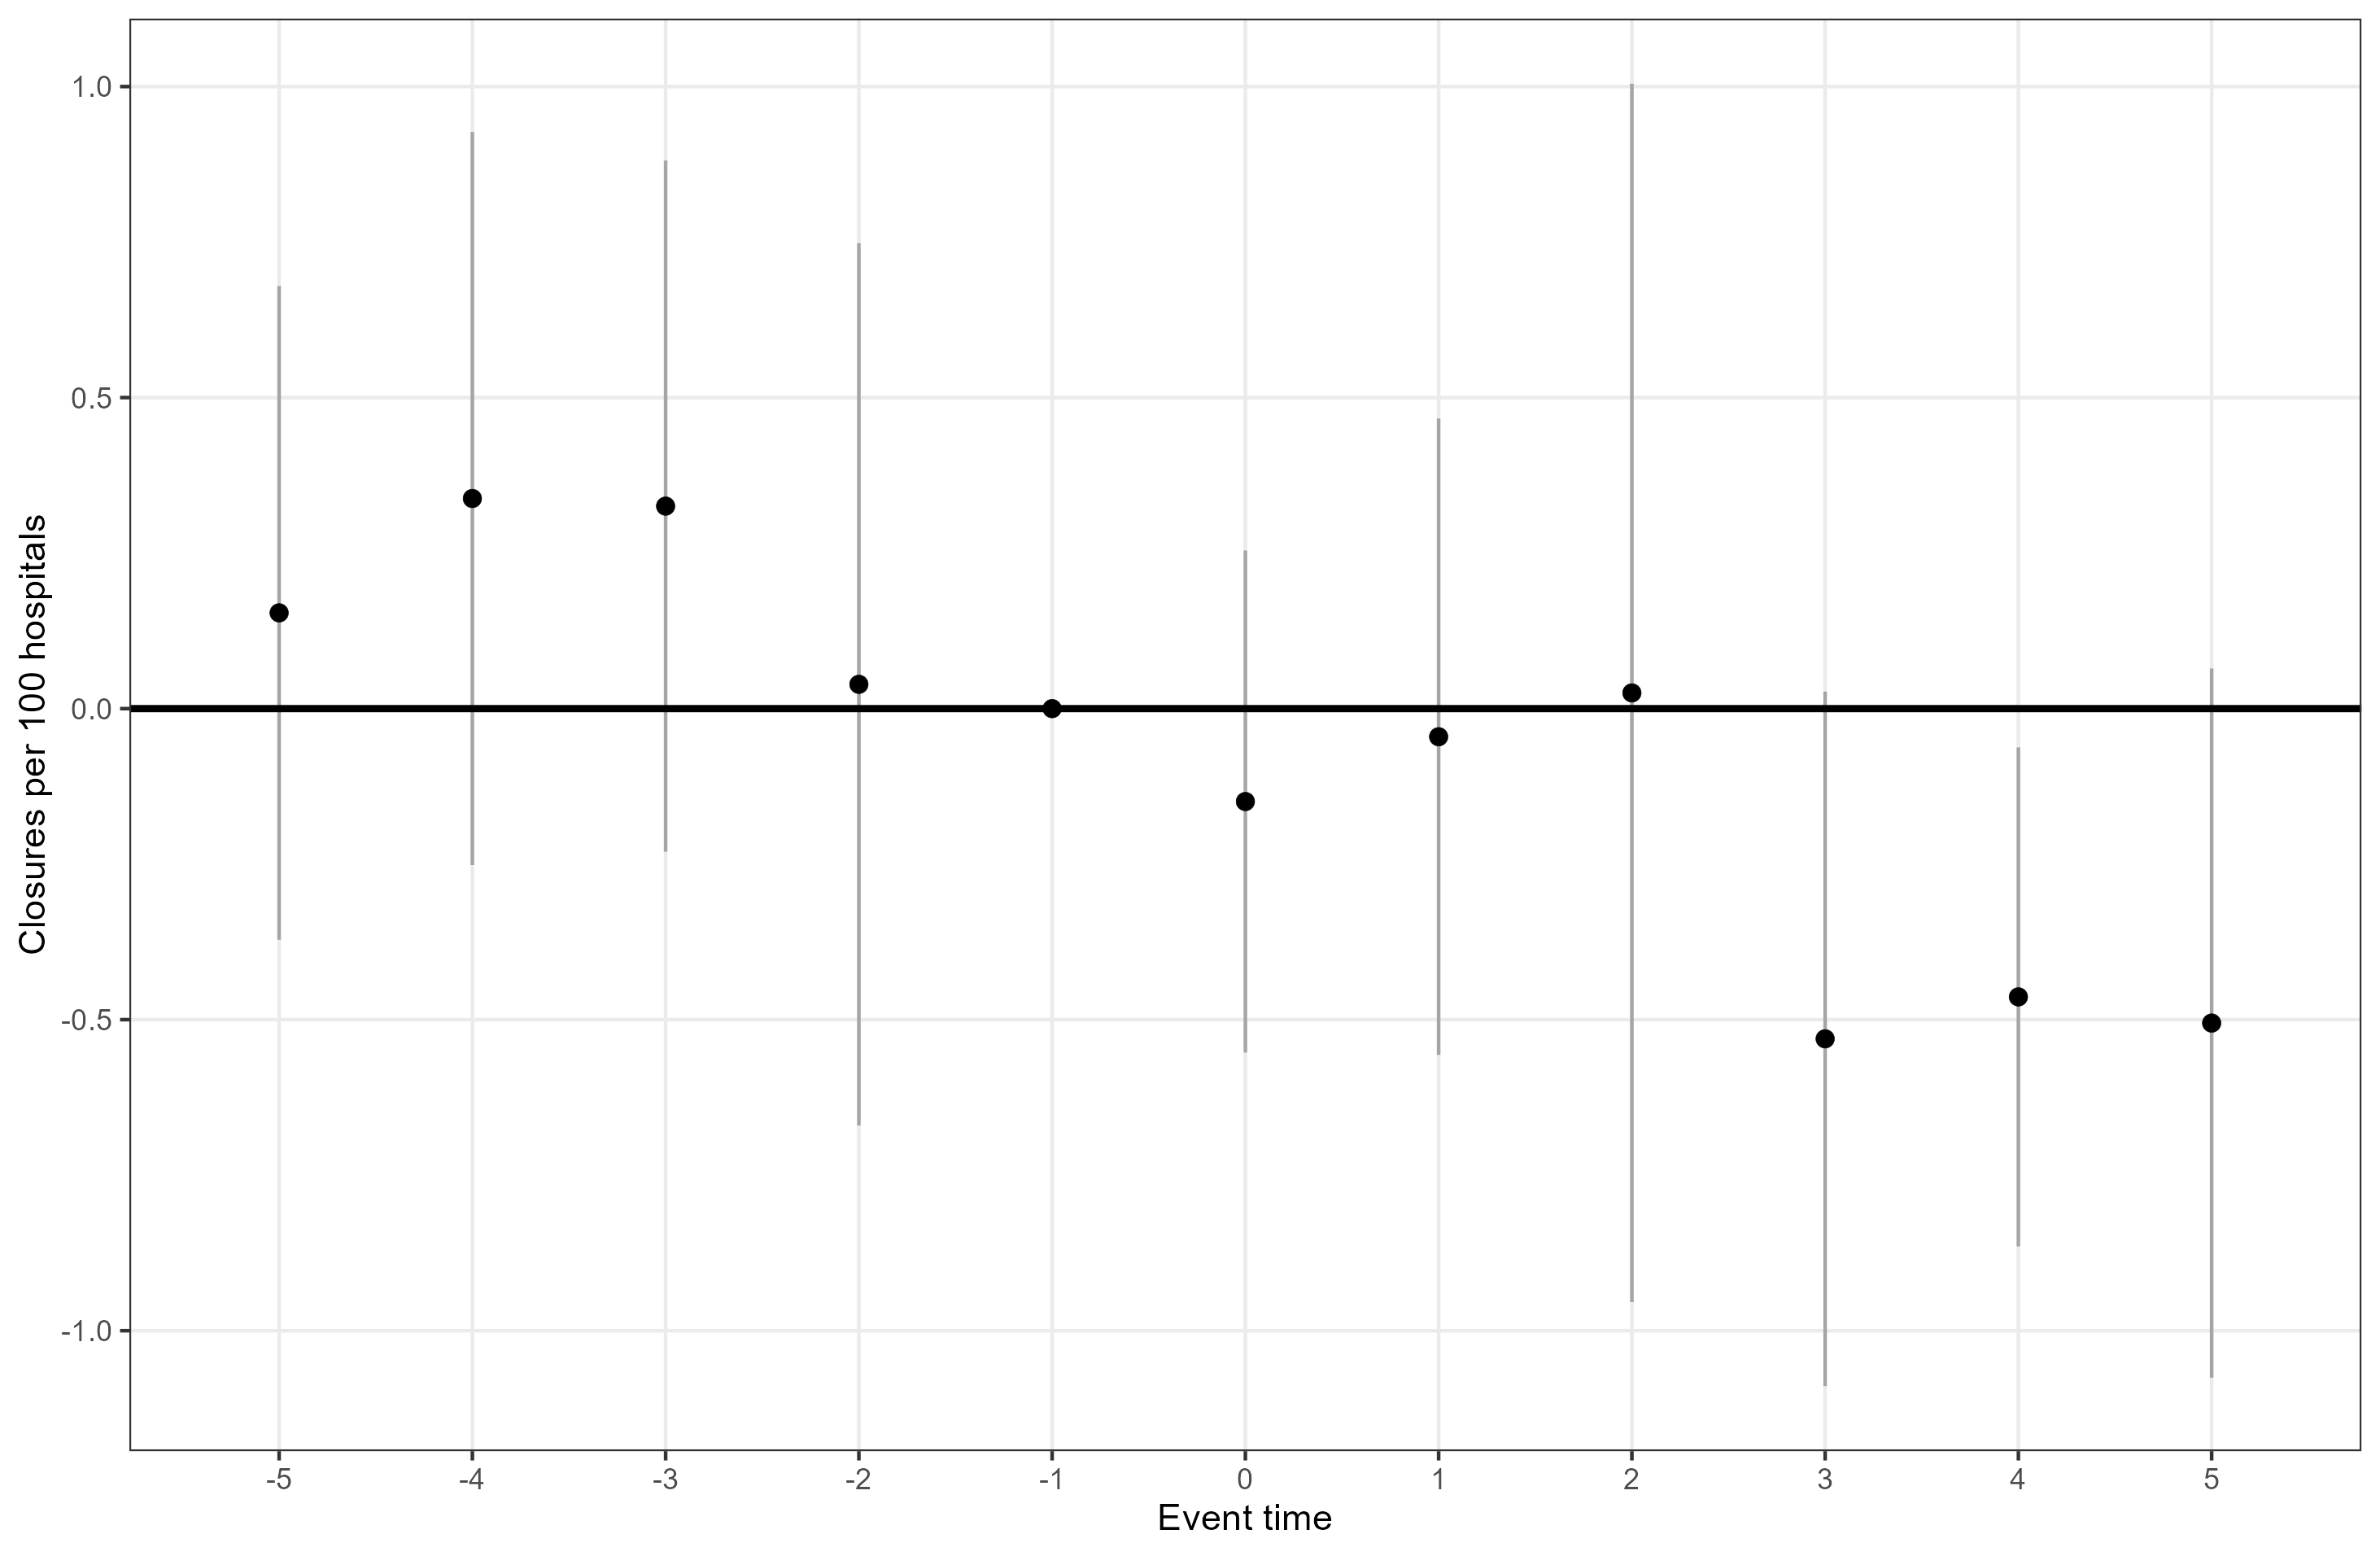
\includegraphics[width=0.48\textwidth]{../results/closure-rate-cs.png} &
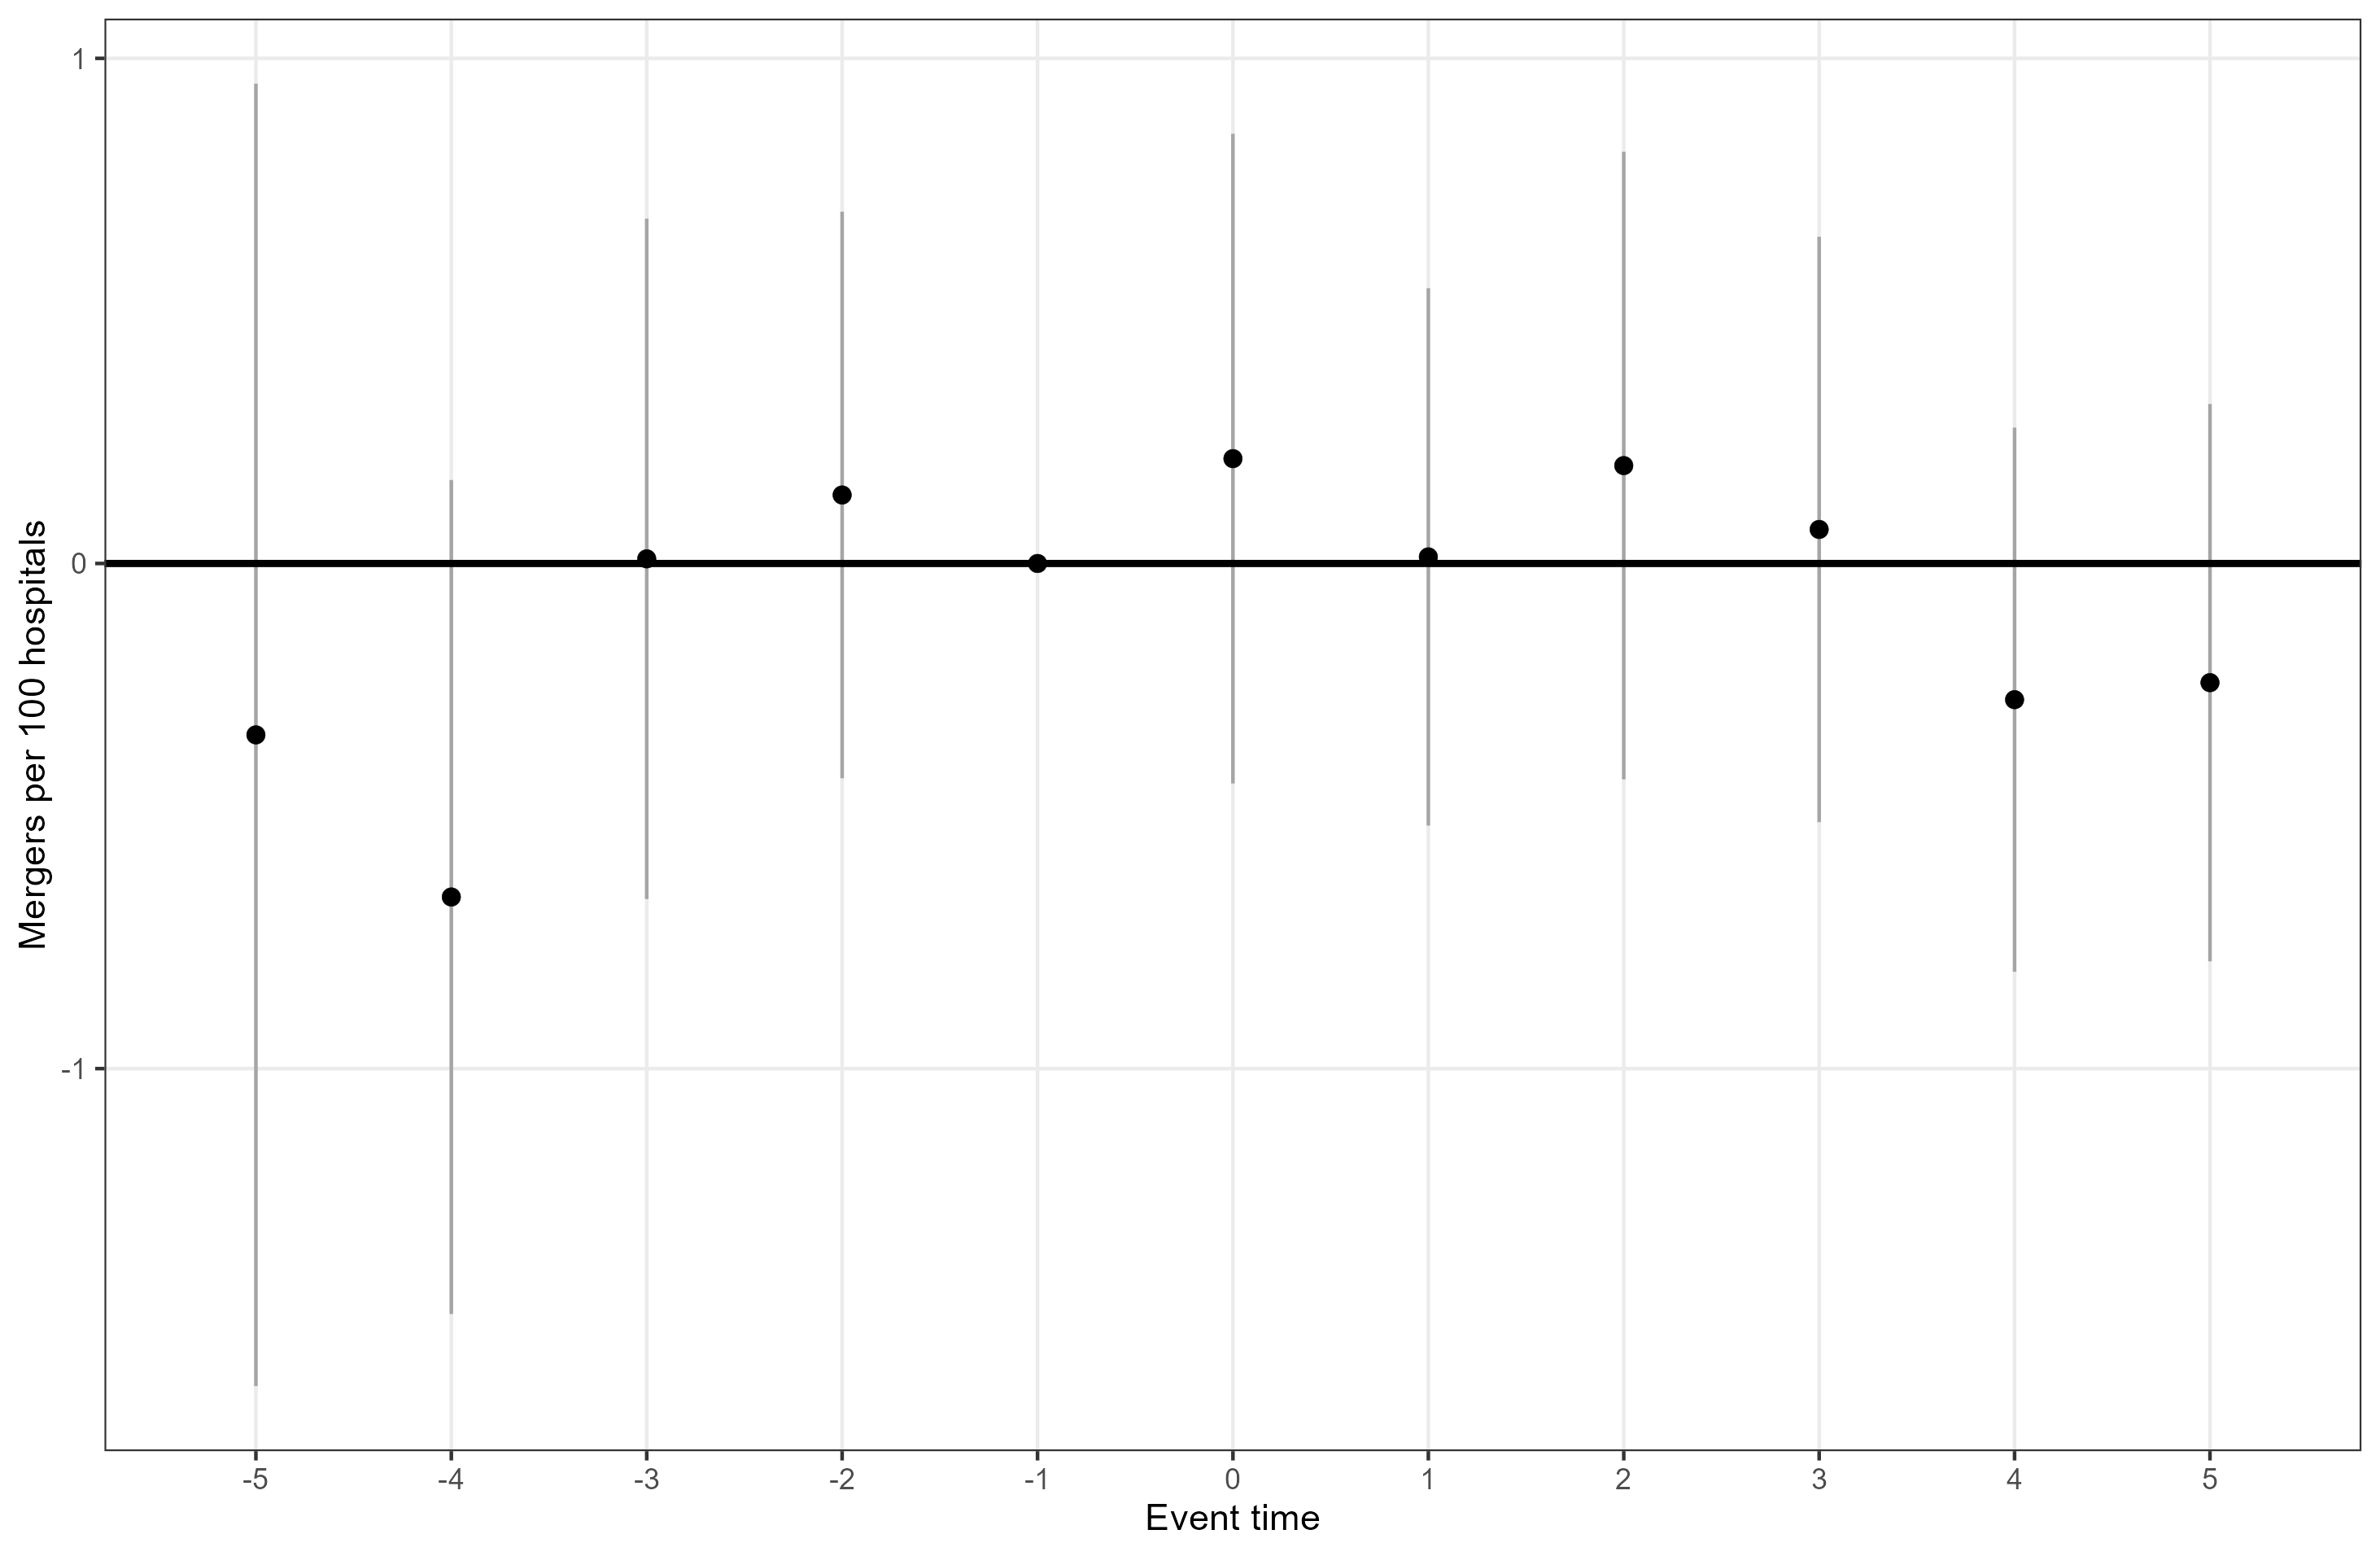
\includegraphics[width=0.48\textwidth]{../results/merger-rate-cs.png} \\
\small (a) Closures (per 100 hospitals) & \small (b) Mergers (per 100 hospitals) \\[0.5cm]
\multicolumn{2}{c}{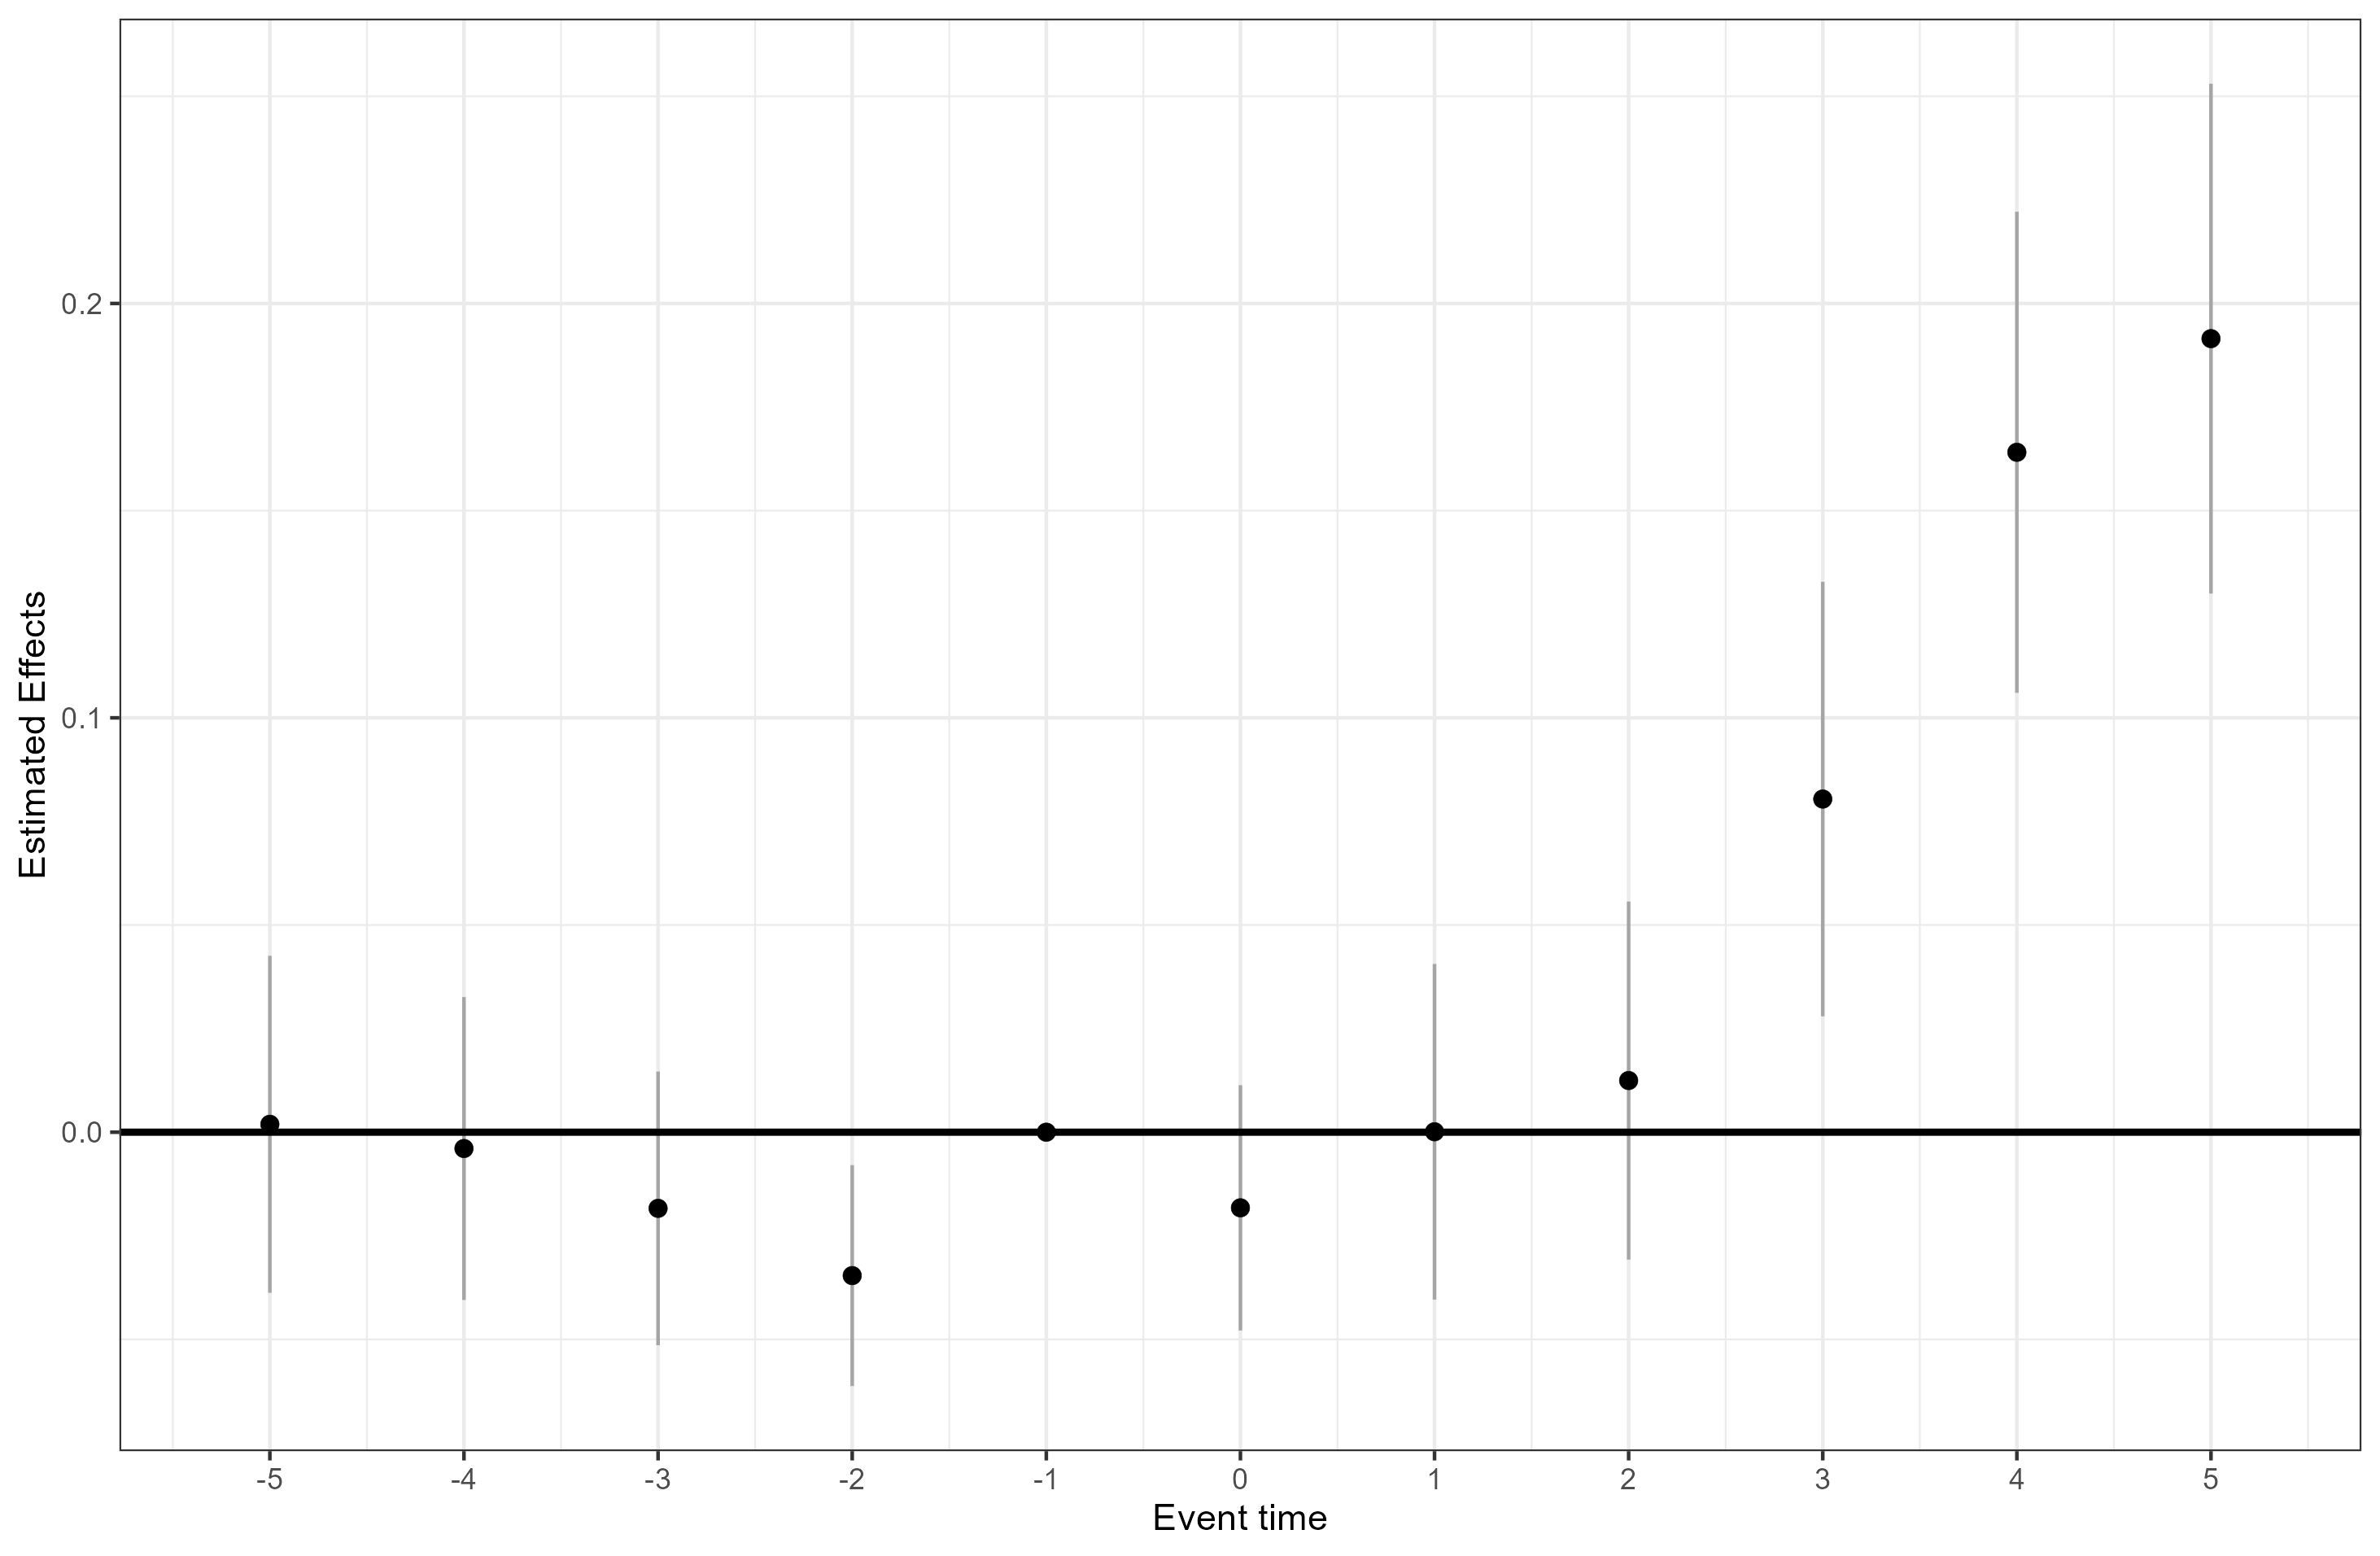
\includegraphics[width=0.48\textwidth]{../results/system-cs.png}} \\
\multicolumn{2}{c}{\small (c) System Membership}
\end{tabular}
\end{minipage}
\end{figure}

\clearpage

\begin{figure}[!h]
\centering
\begin{minipage}[h]{6in}
\caption[CS Event Studies: Visits and Births]{\textbf{CS Event-Study Estimates: Outpatient Visits, Emergency Department Visits, and Births}\footnote{Callaway--Sant'Anna event-study estimates with 95\% confidence intervals by years relative to designation, state-timing design (cohorts 1999--2001), not-yet-treated control group, universal base period. Visit outcomes are annual counts per pre-designation bed; births are annual counts.}}
\label{fig:cs-visits}
\begin{tabular}{cc}
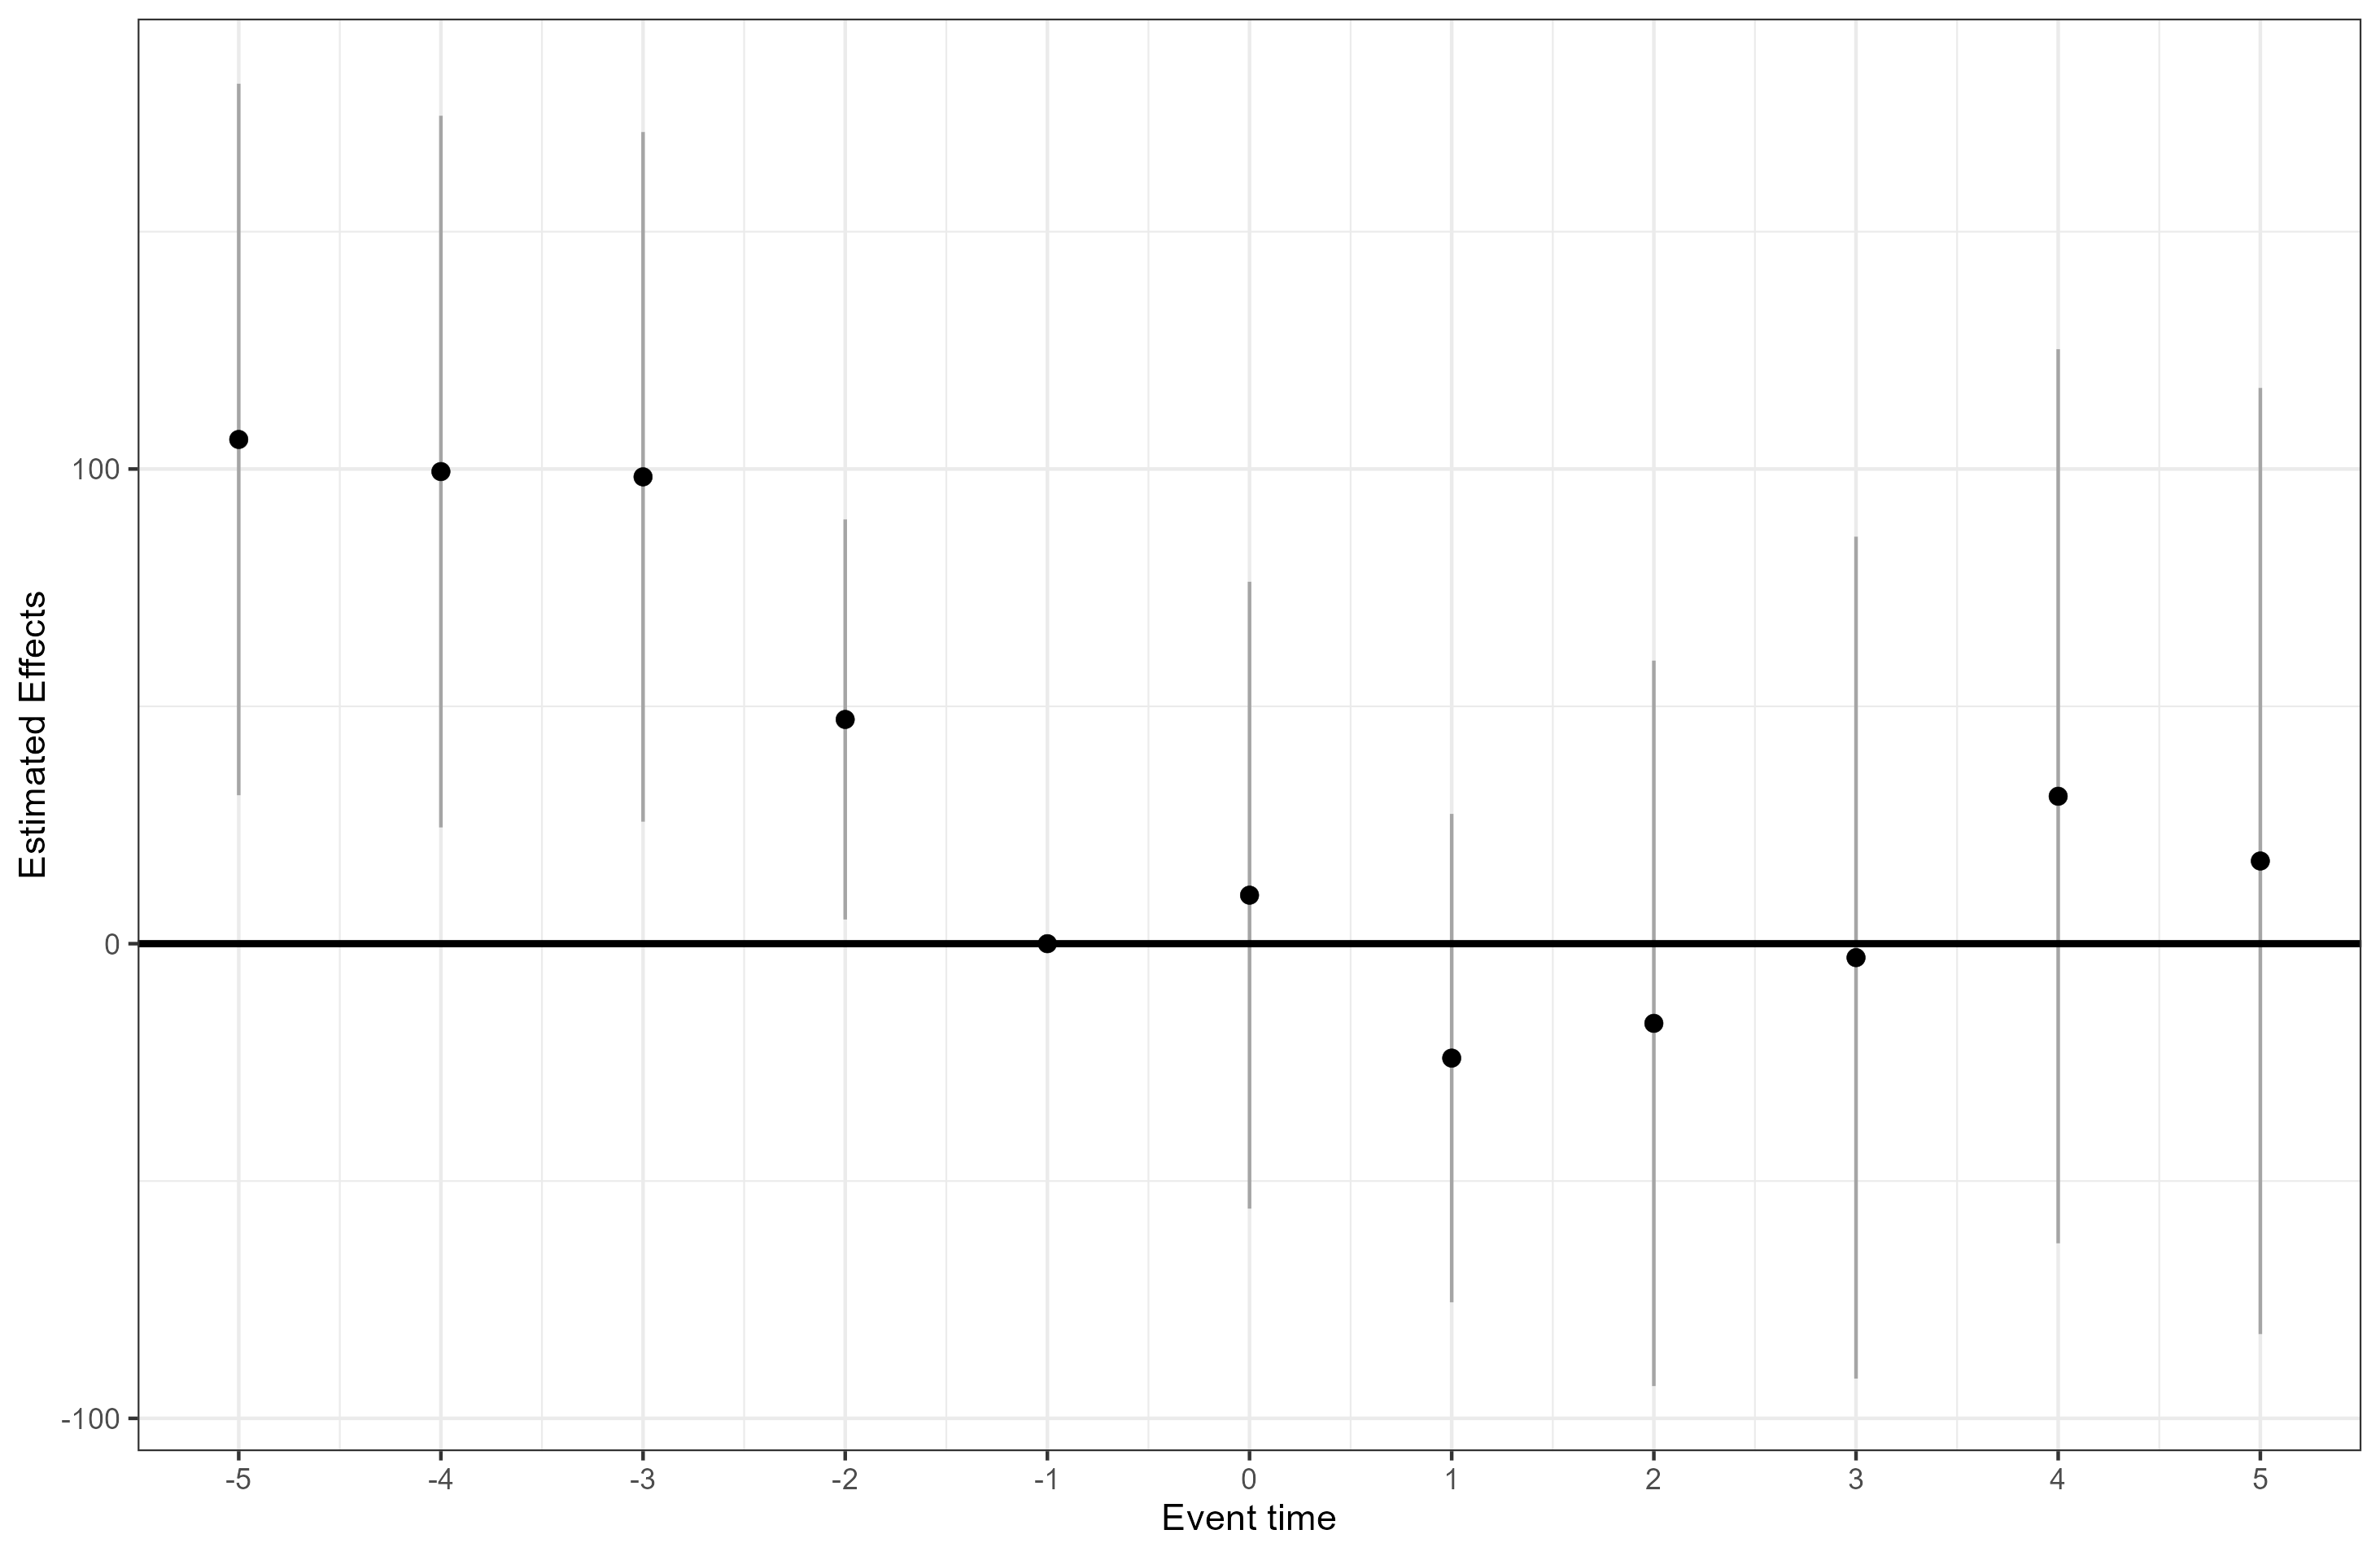
\includegraphics[width=0.48\textwidth]{../results/opvisits-state-cs.png} &
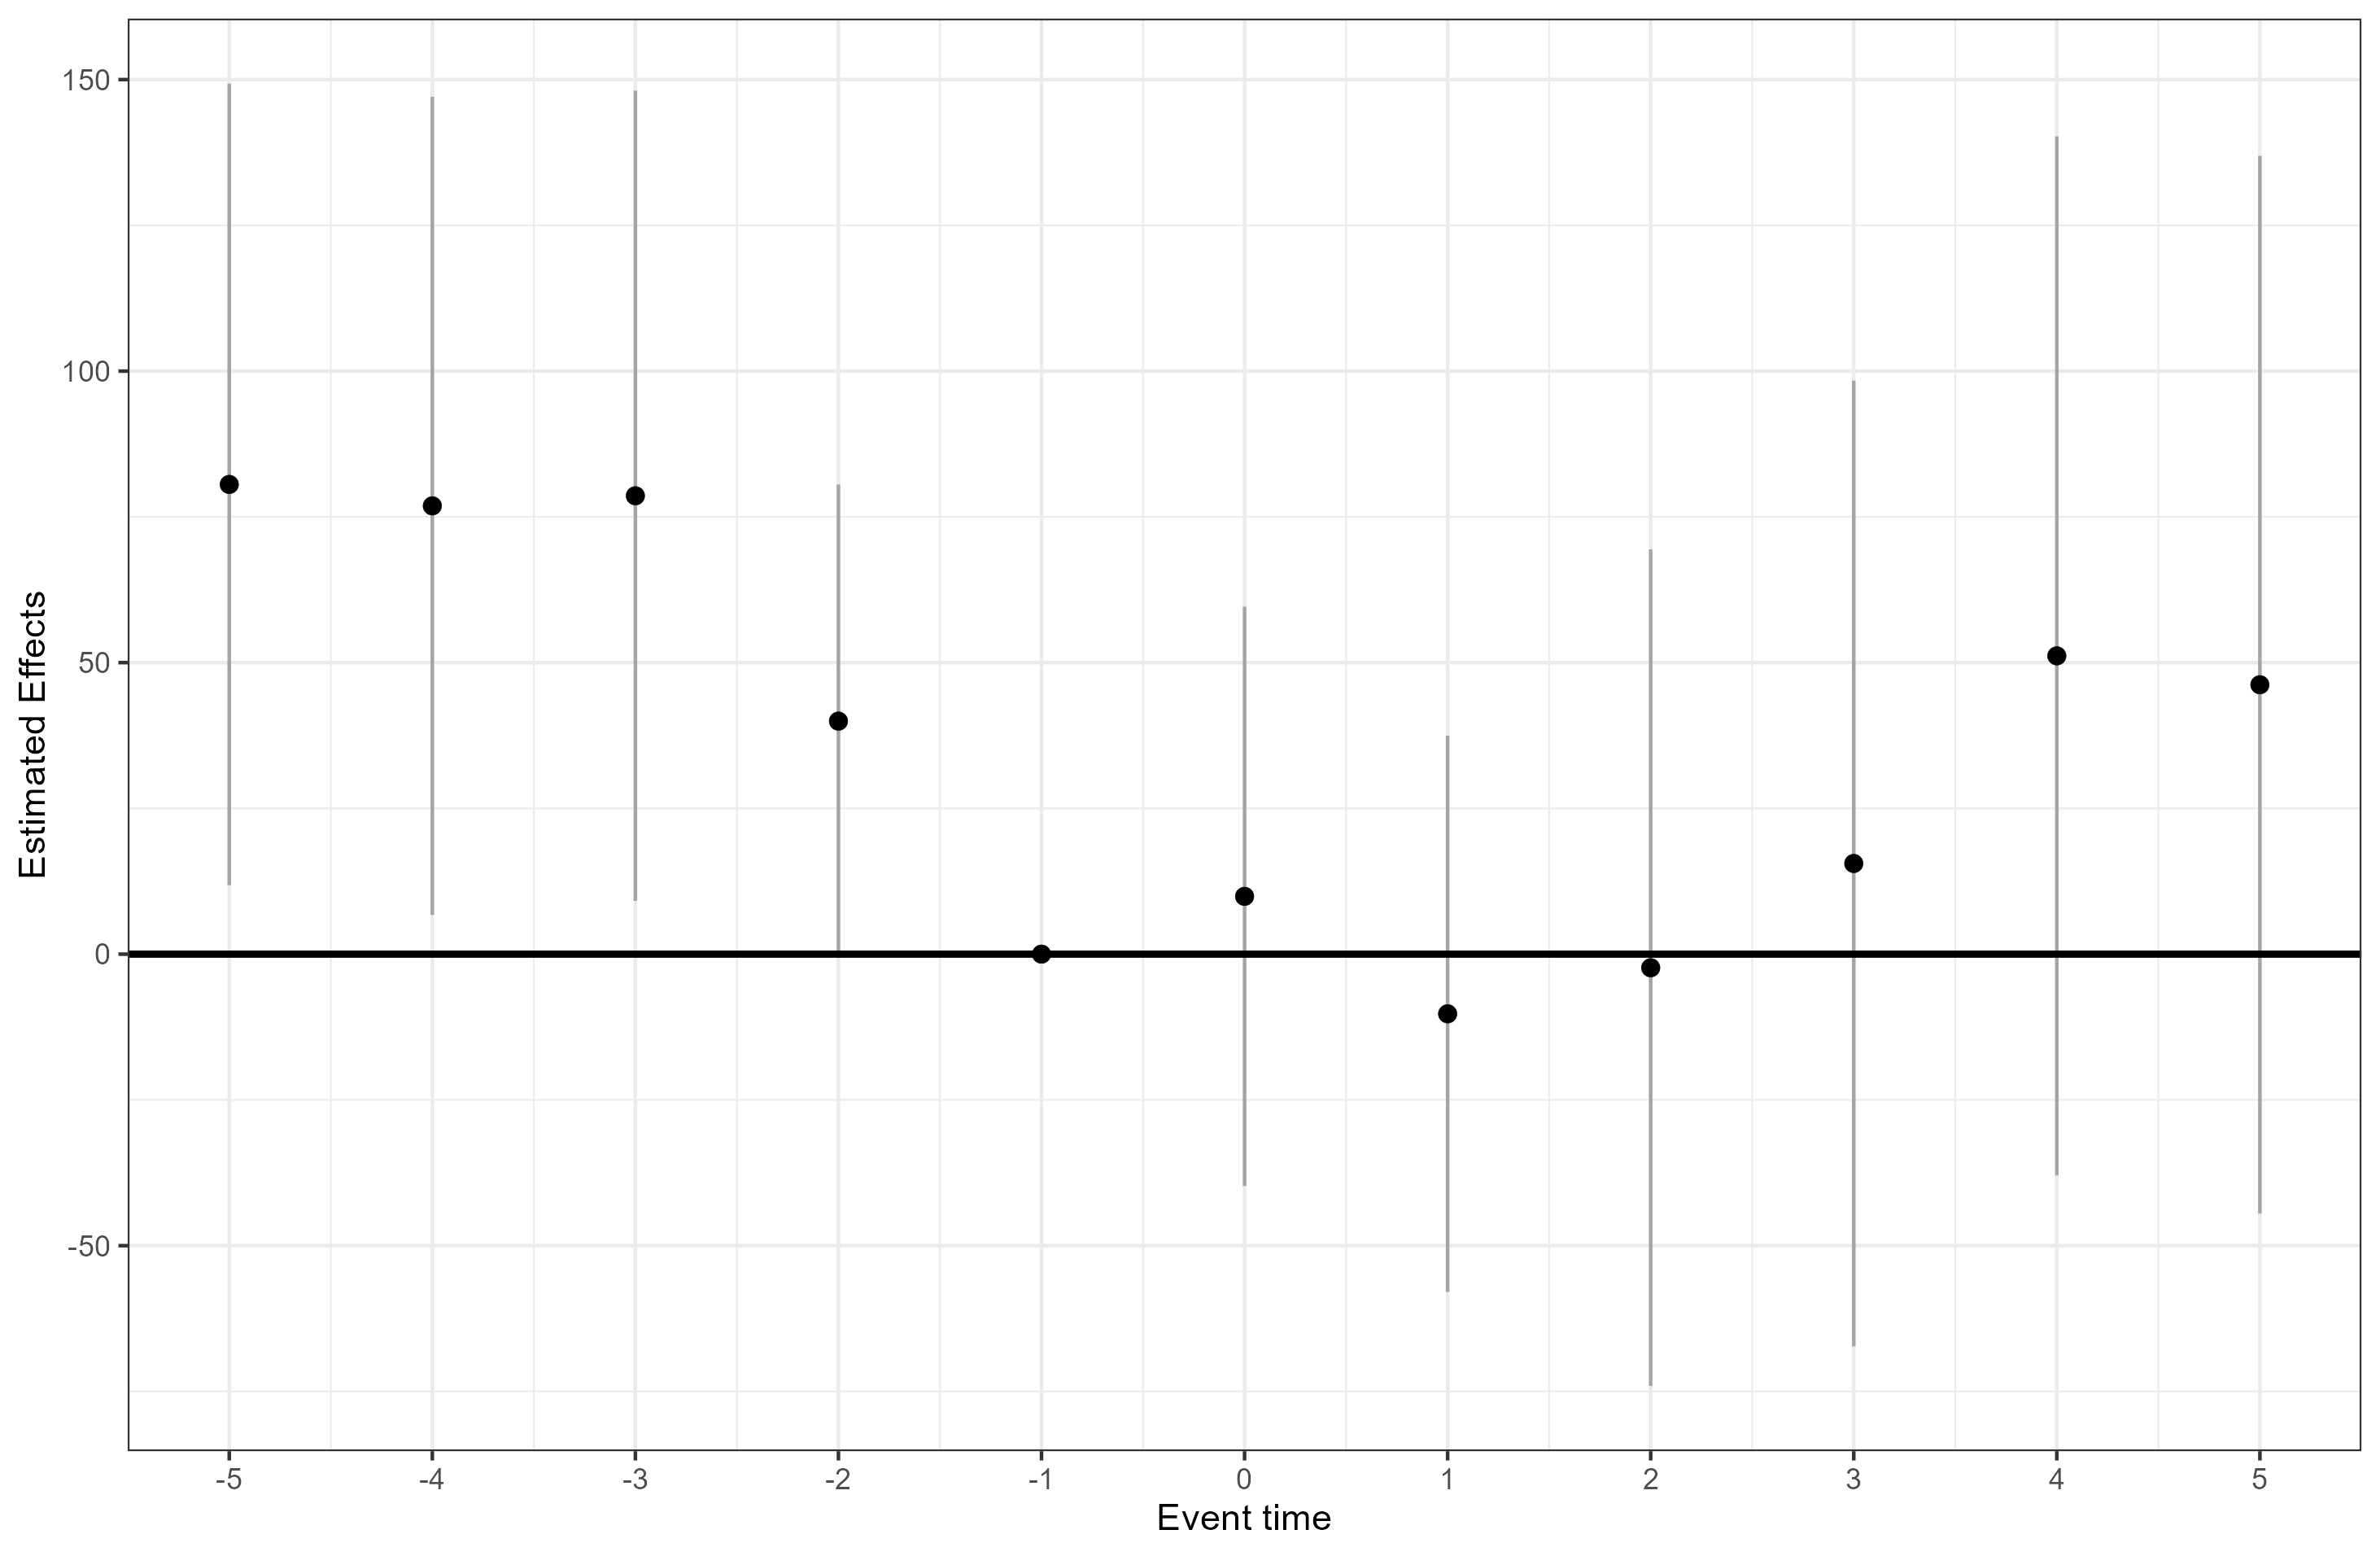
\includegraphics[width=0.48\textwidth]{../results/opvisits-noned-state-cs.png} \\
\small (a) Outpatient Visits per Bed & \small (b) Non-ED Outpatient Visits per Bed \\[0.5cm]
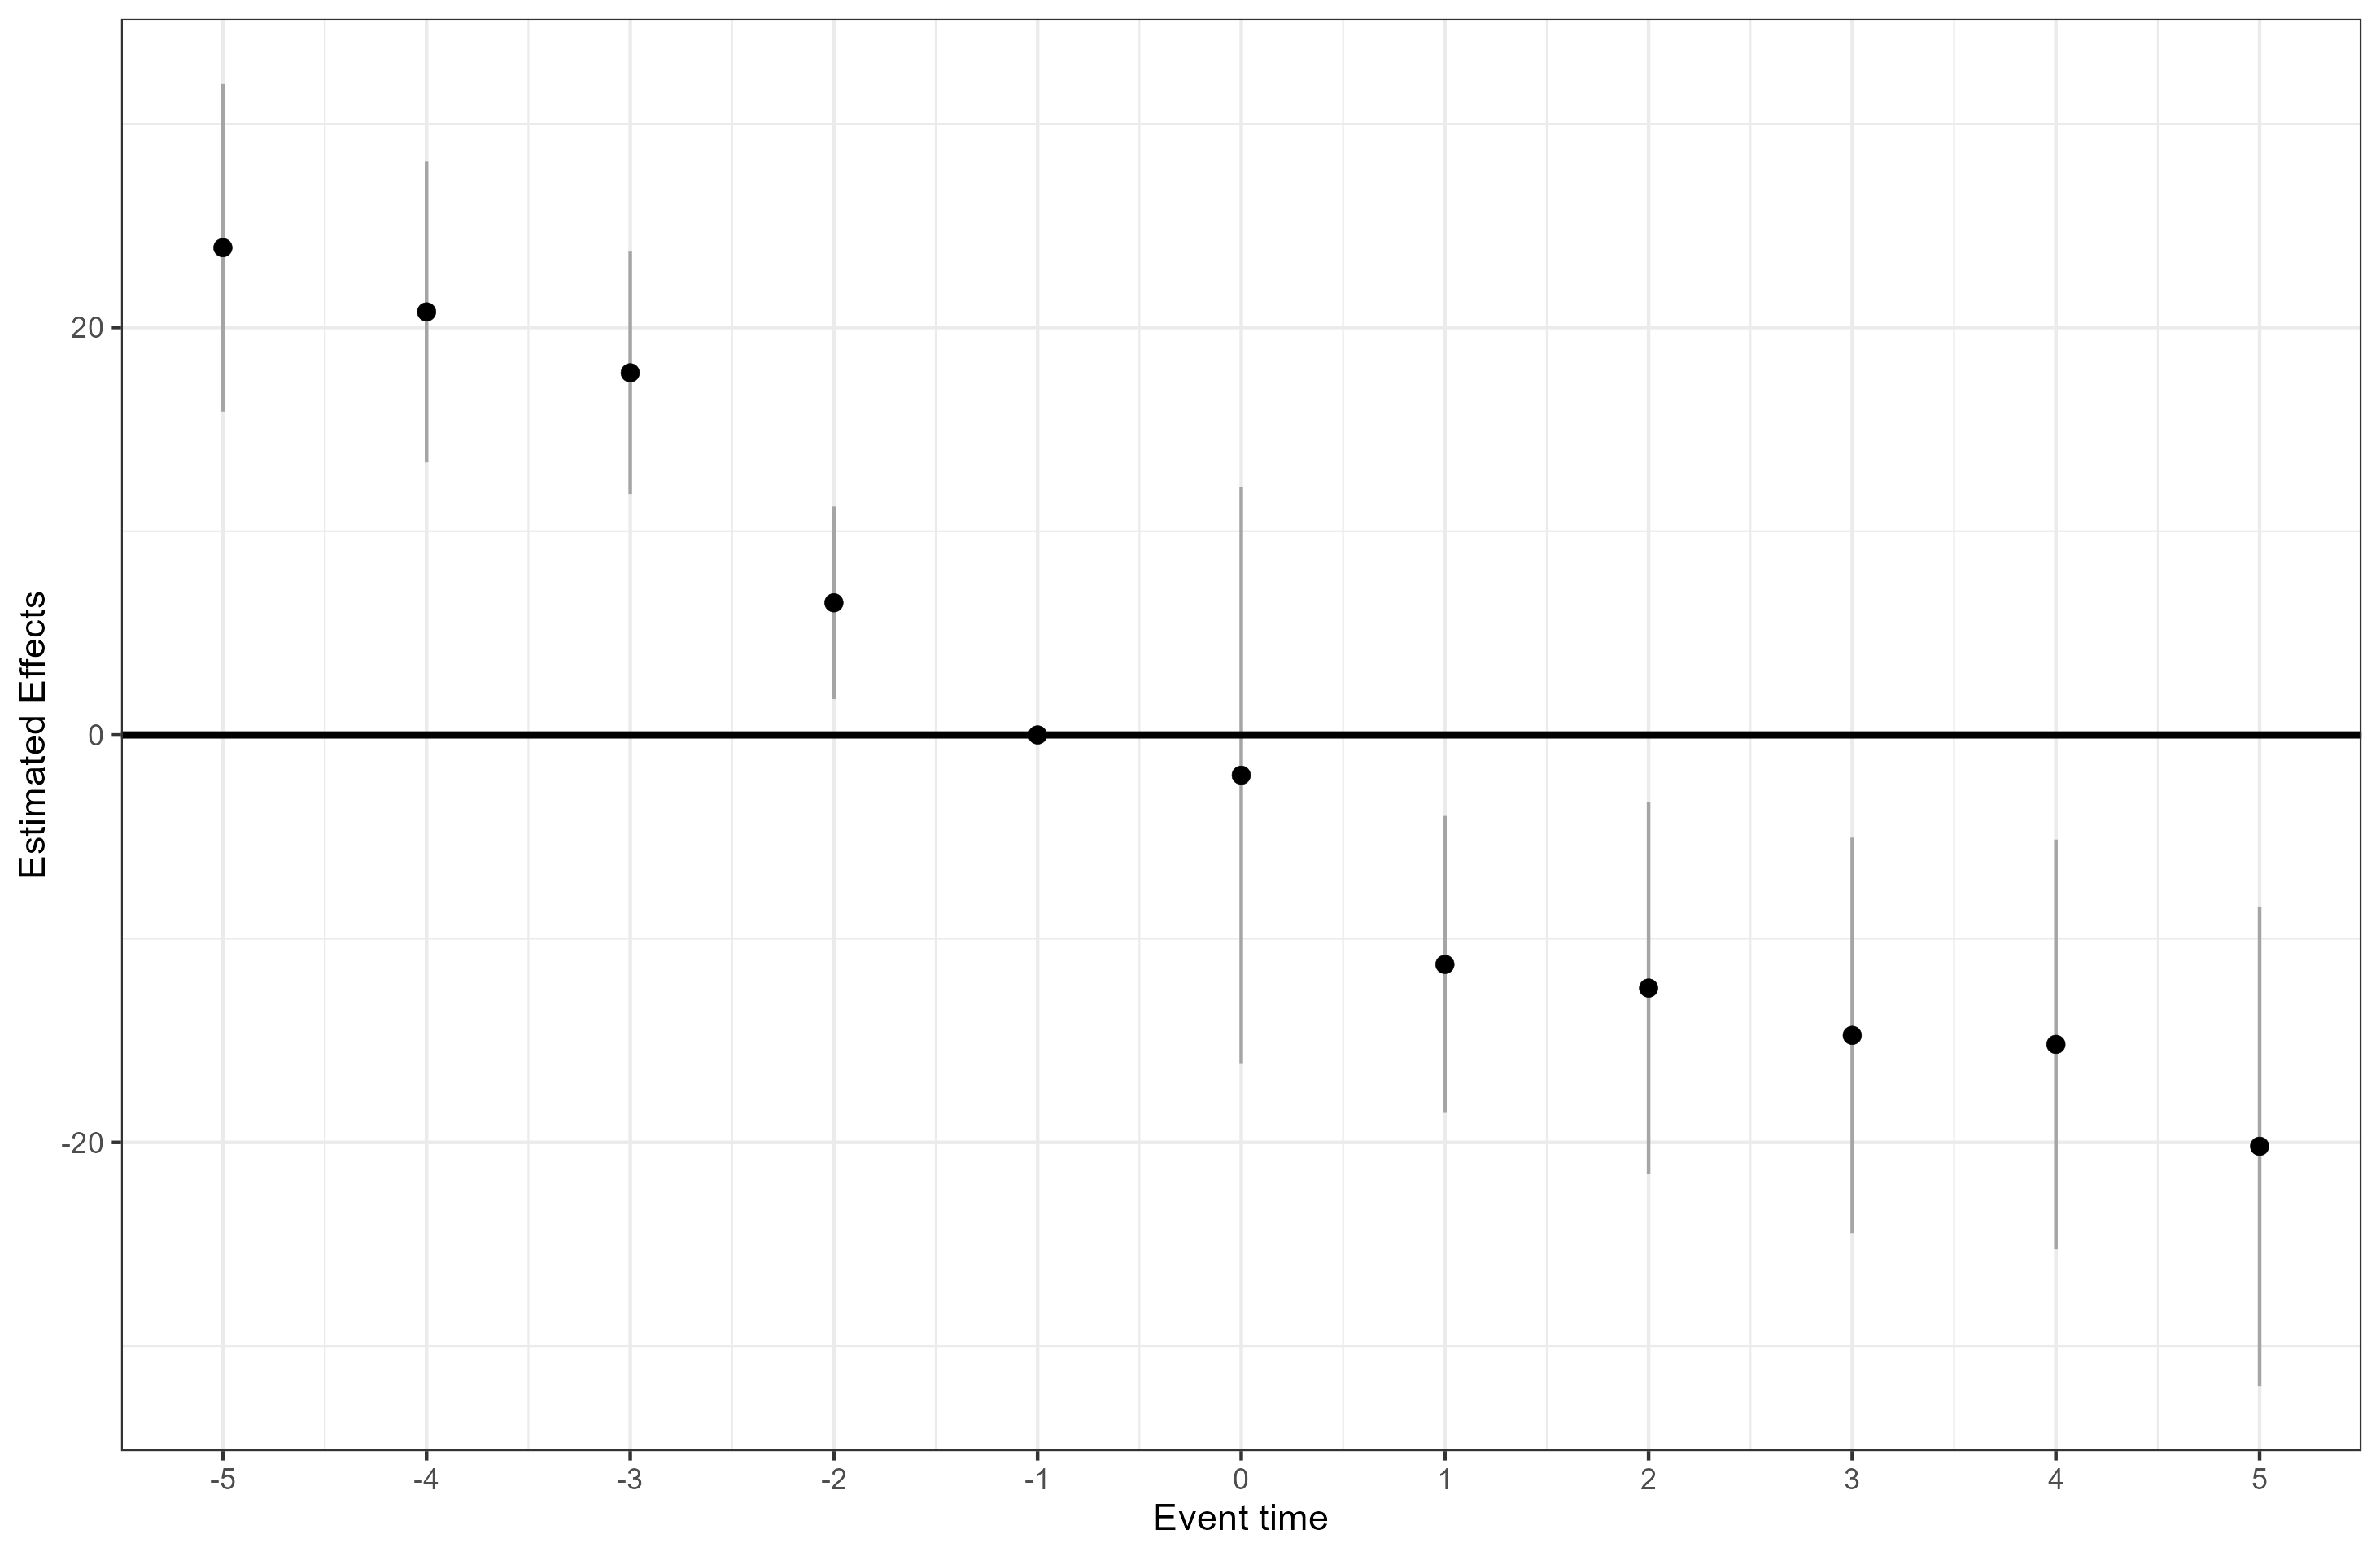
\includegraphics[width=0.48\textwidth]{../results/edvisits-state-cs.png} &
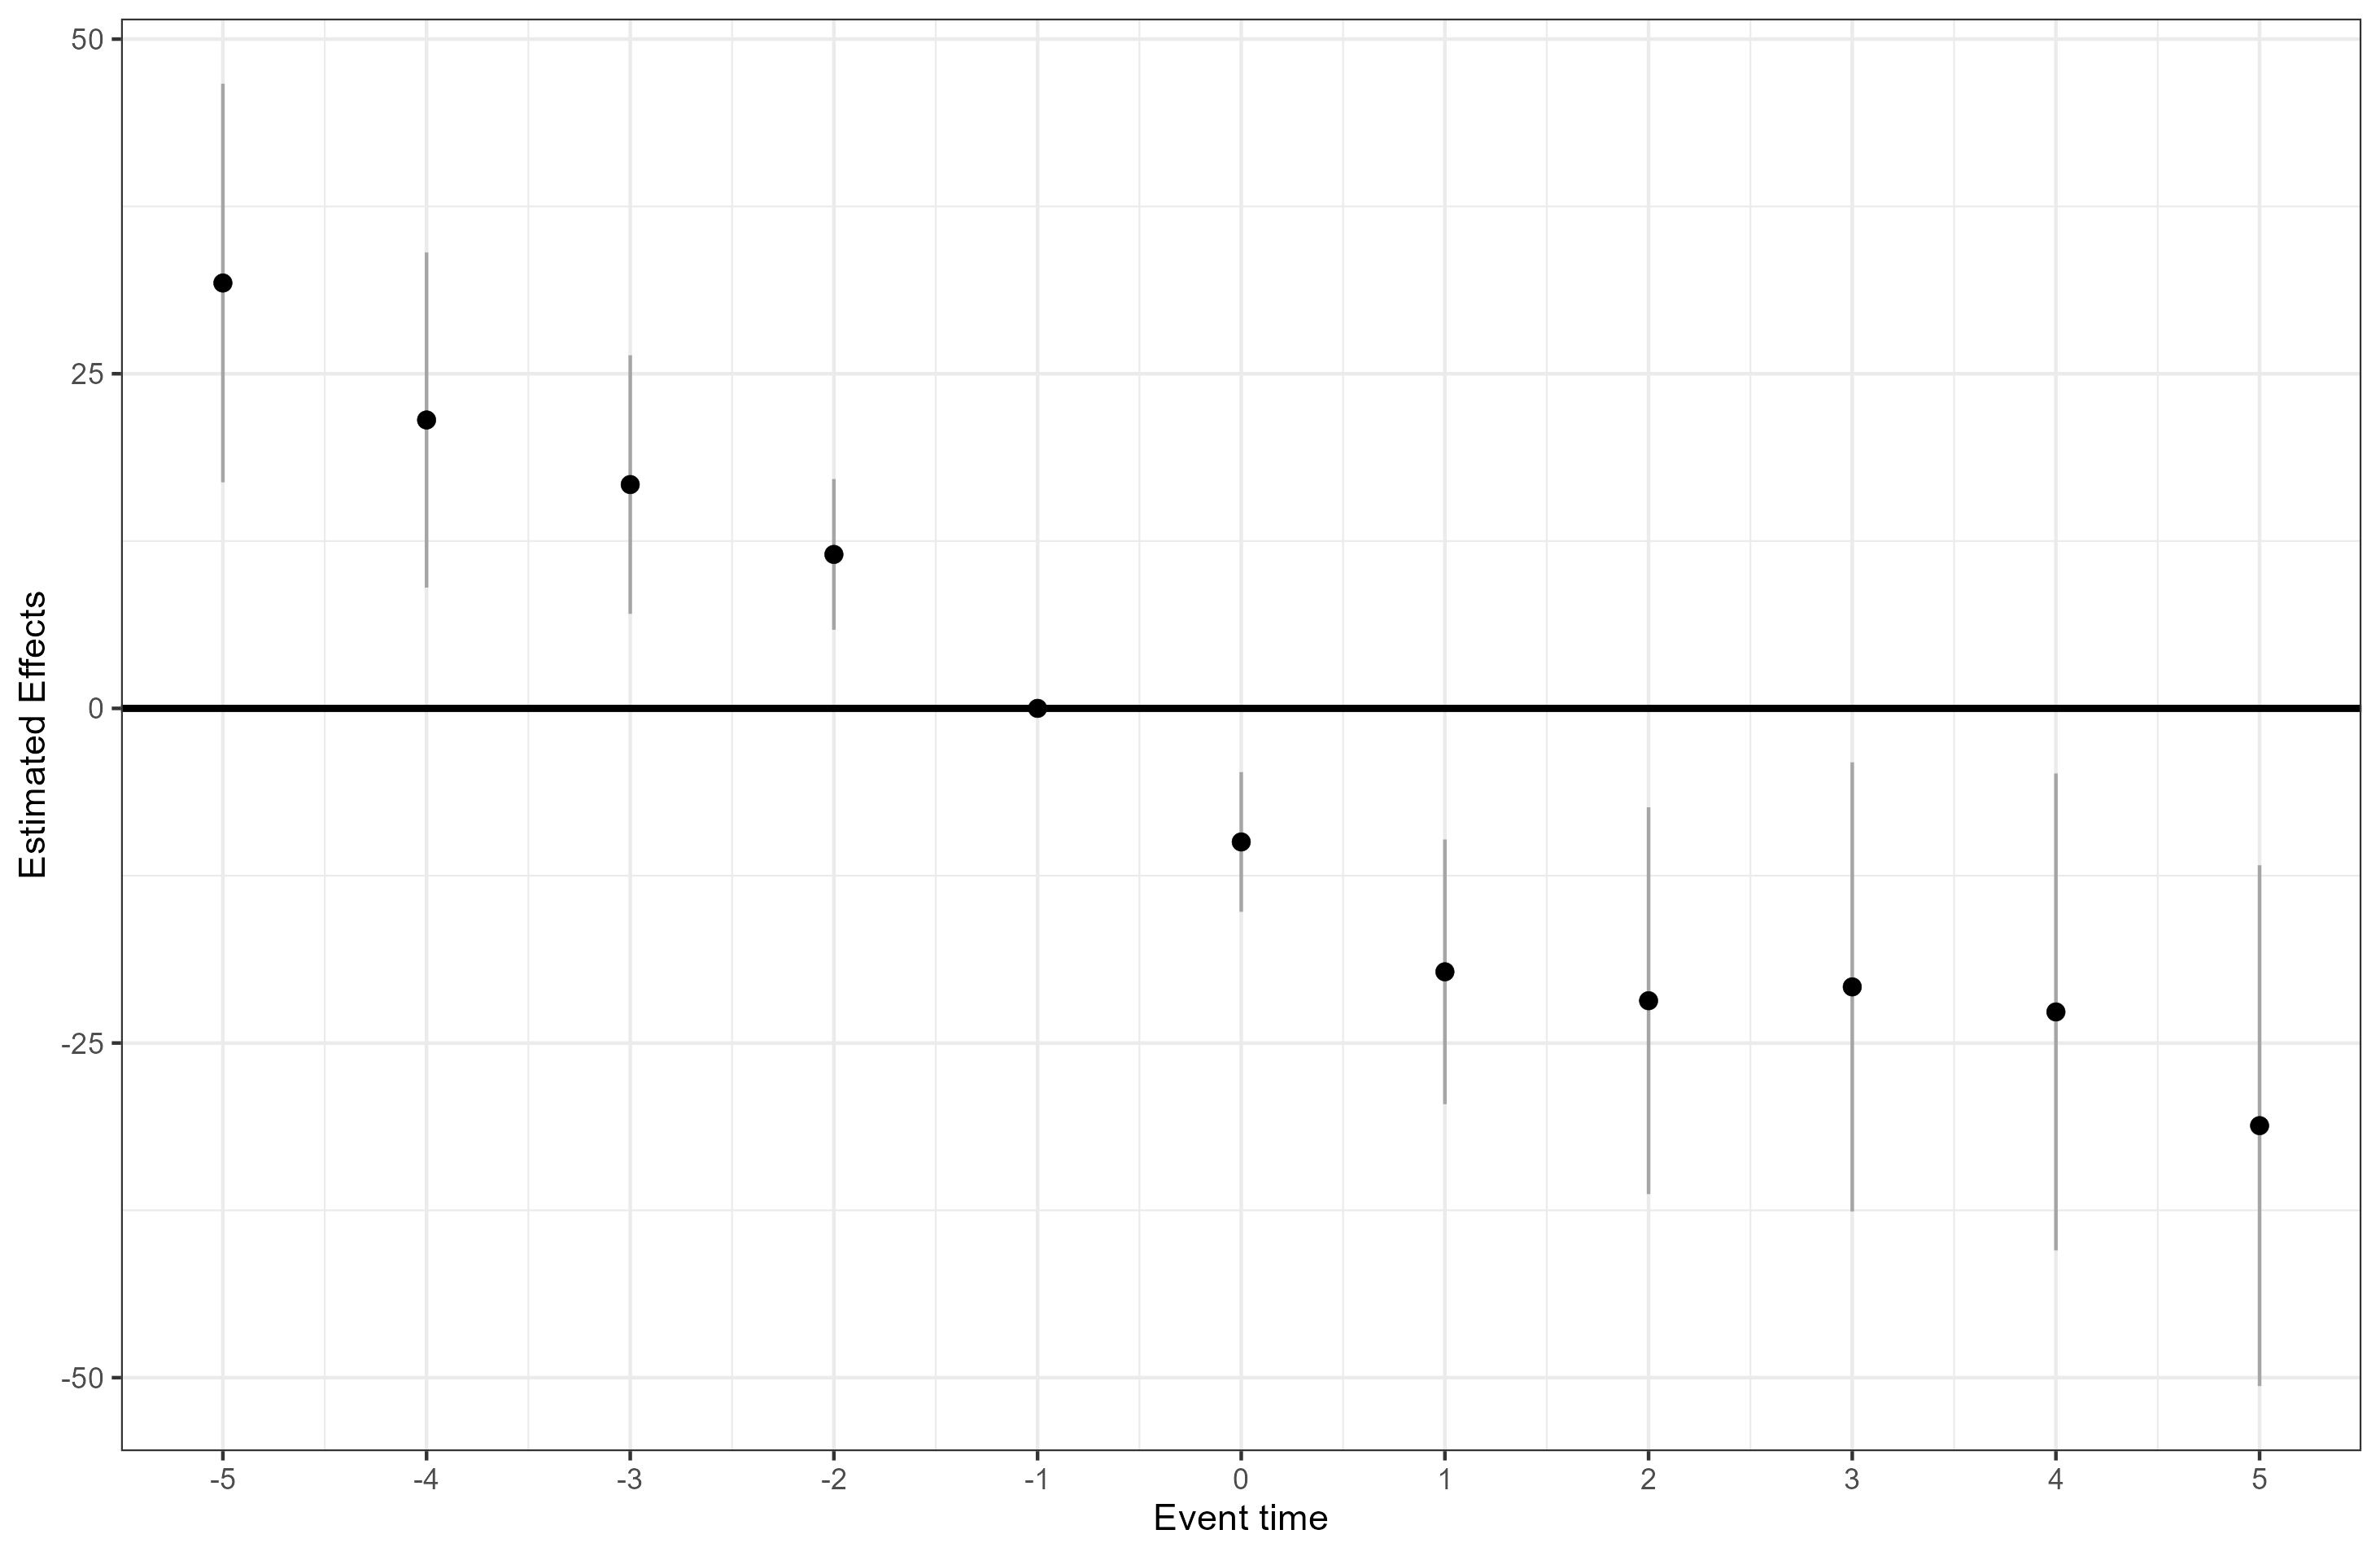
\includegraphics[width=0.48\textwidth]{../results/births-state-cs.png} \\
\small (c) Emergency Department Visits per Bed & \small (d) Births
\end{tabular}
\end{minipage}
\end{figure}

\clearpage

\begin{figure}[!h]
\centering
\begin{minipage}[h]{6in}
\caption[CS Event Studies (Eligibility): Financial]{\textbf{CS Event-Study Estimates (Eligibility-Restricted): Financial Performance and Capital}\footnote{Callaway--Sant'Anna event-study estimates with 95\% confidence intervals by years relative to designation, eligibility-restricted design (cohorts 1999--2005), not-yet-treated control group, universal base period. Revenue and expense measures are in thousands of 2010 dollars per bed.}}
\label{fig:elig-cs-financial}
\begin{tabular}{cc}
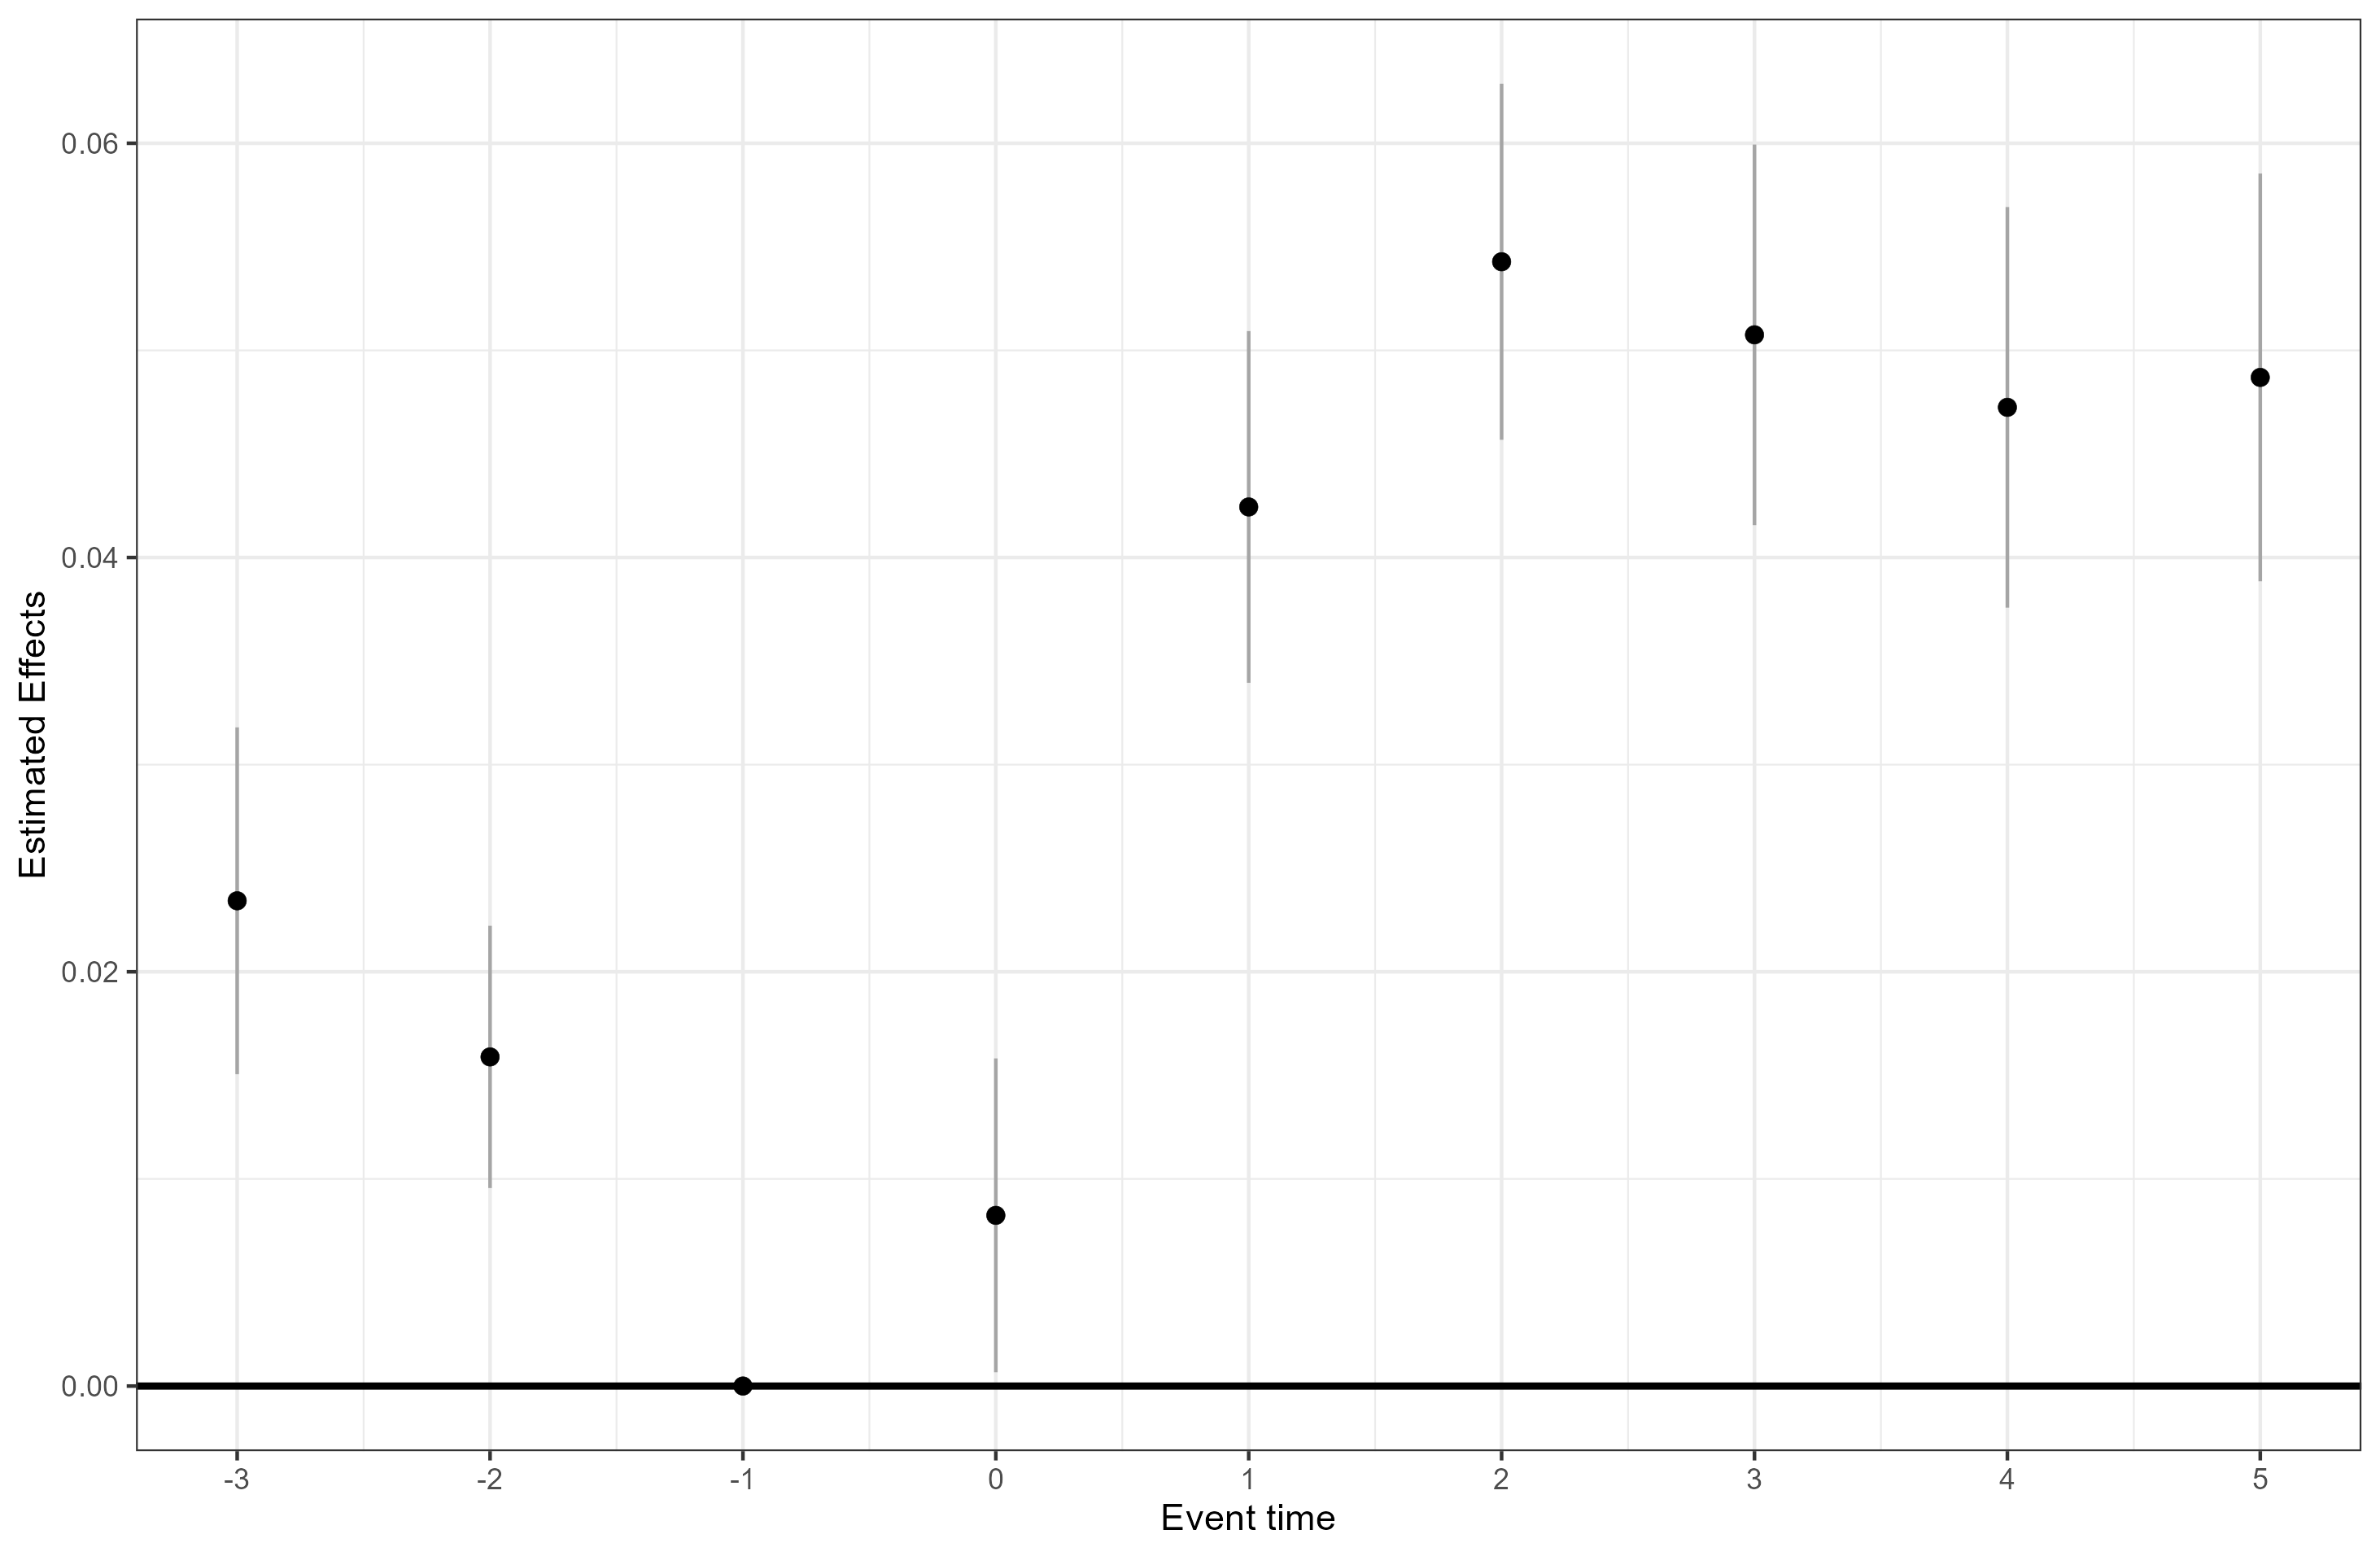
\includegraphics[width=0.48\textwidth]{../results/elig-margin-cs.png} &
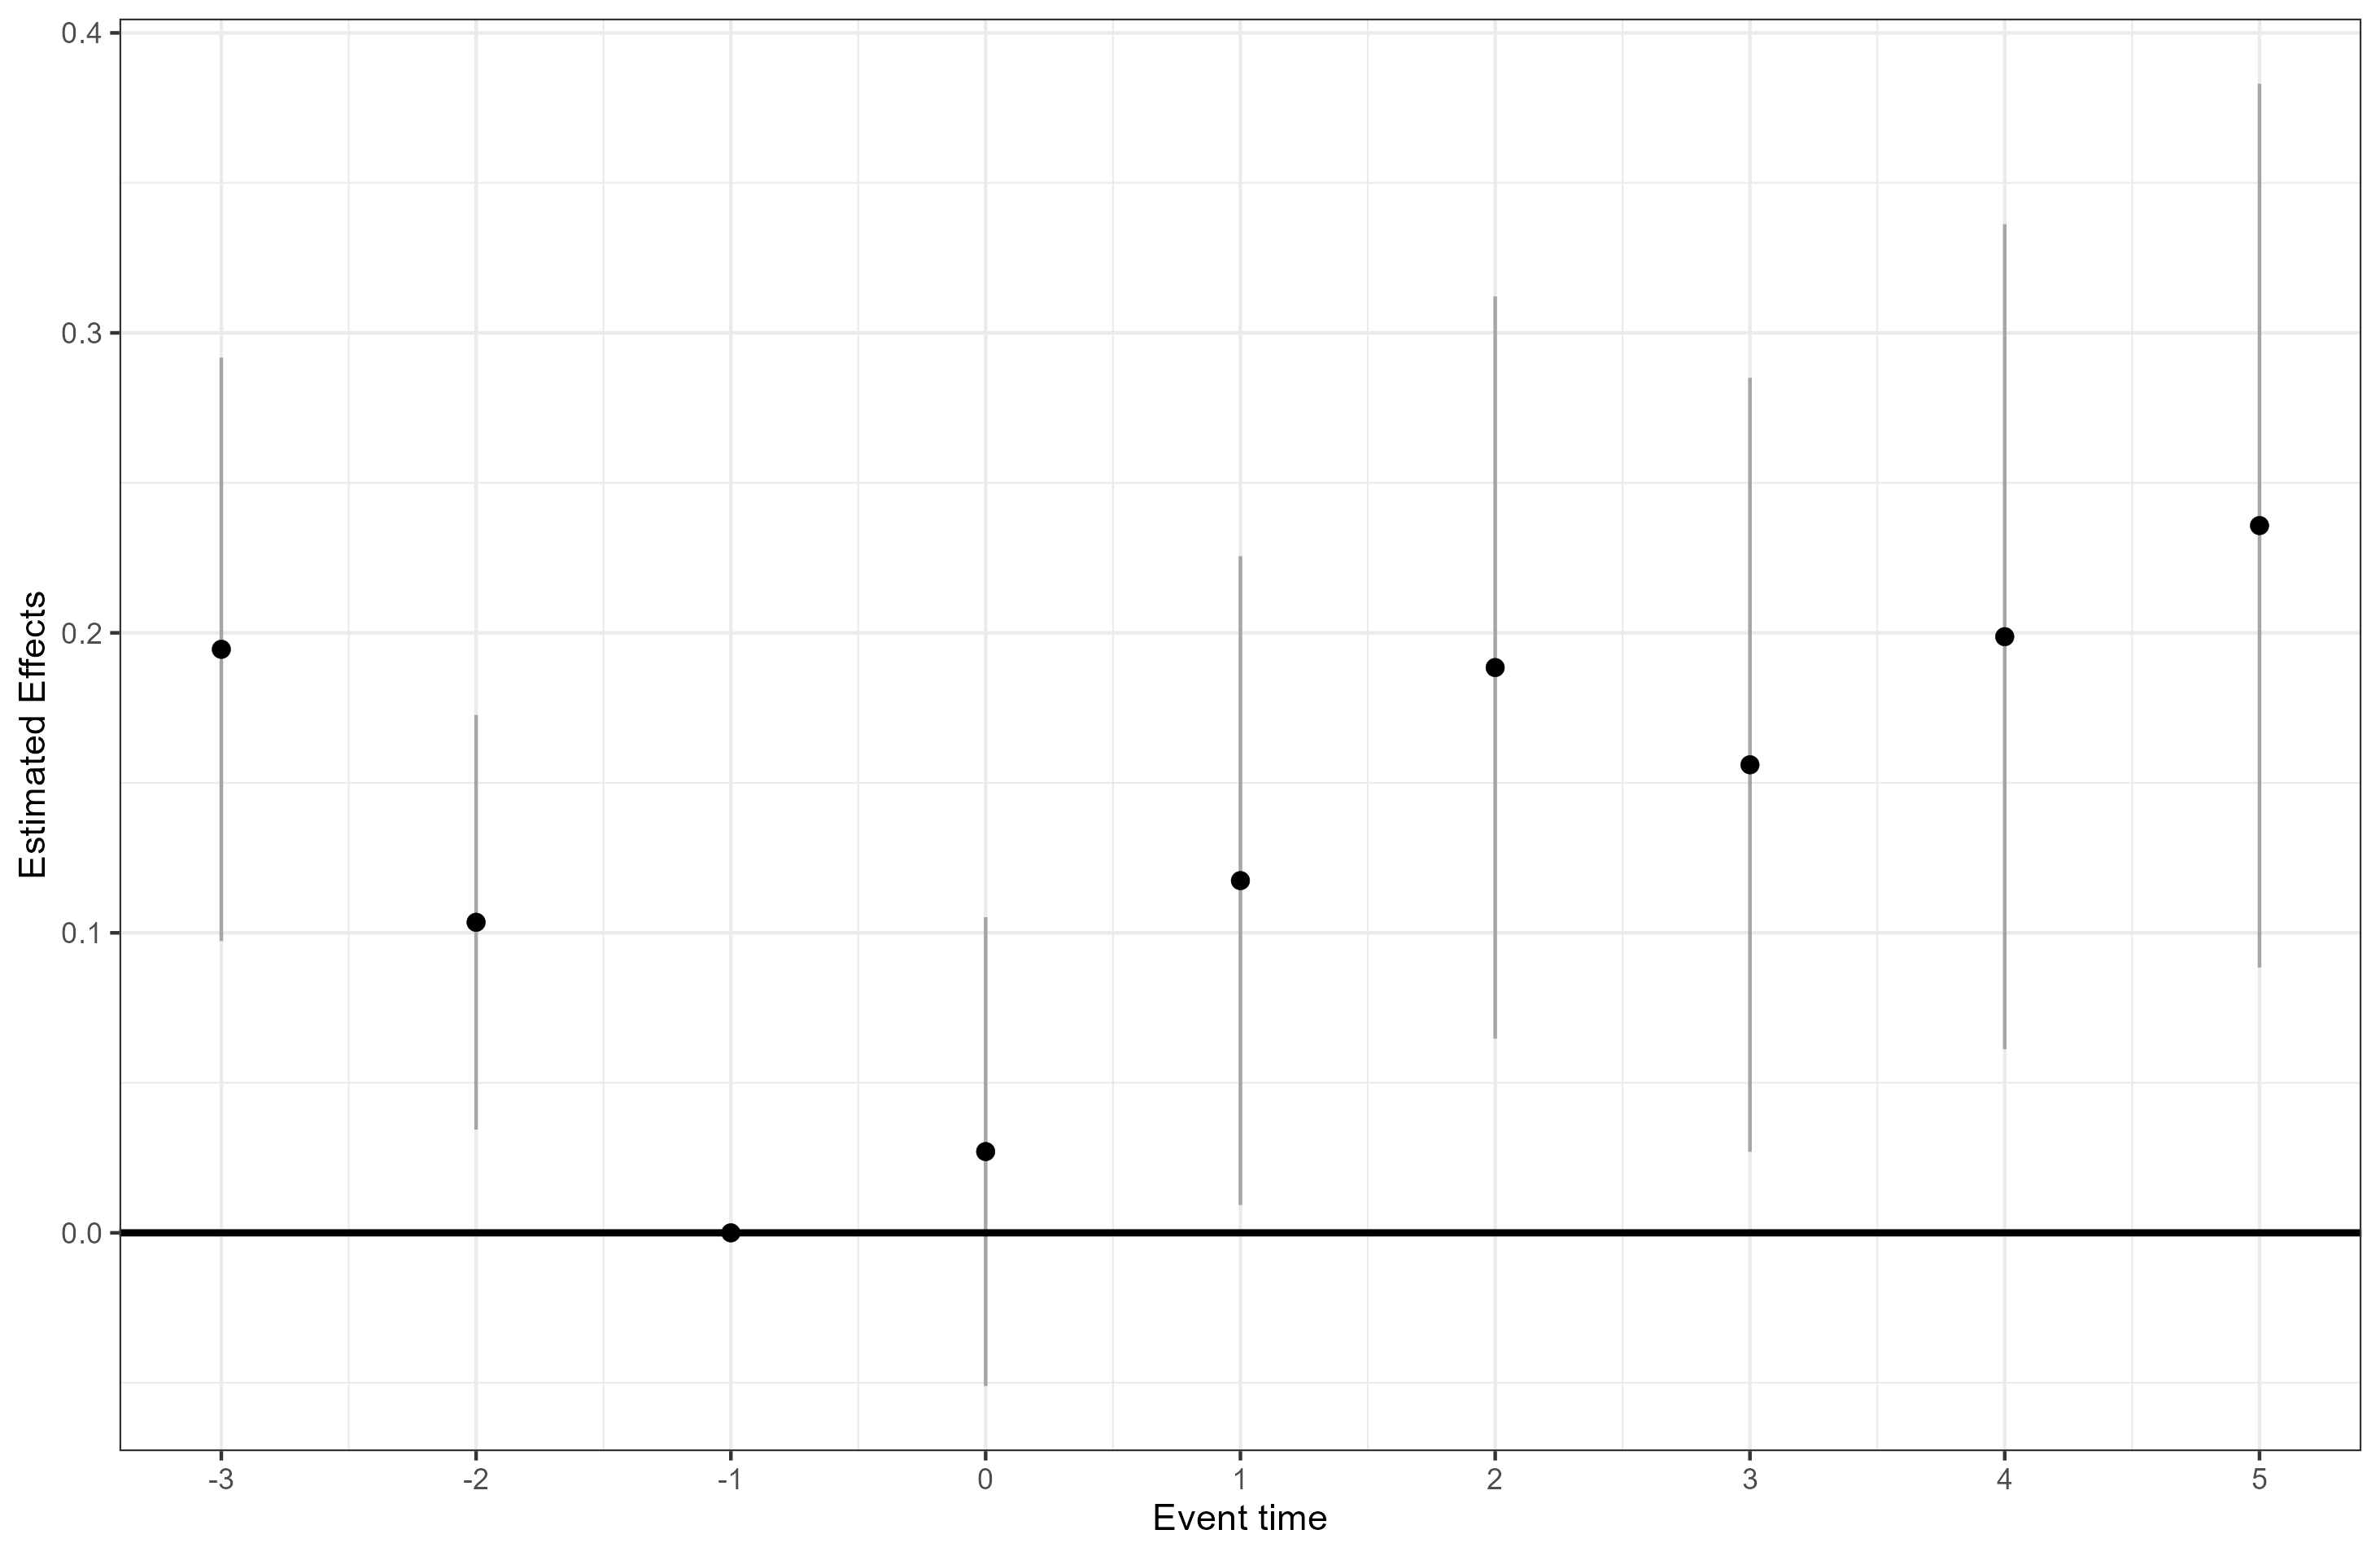
\includegraphics[width=0.48\textwidth]{../results/elig-currentratio-cs.png} \\
\small (a) Operating Margin & \small (b) Current Ratio \\[0.5cm]
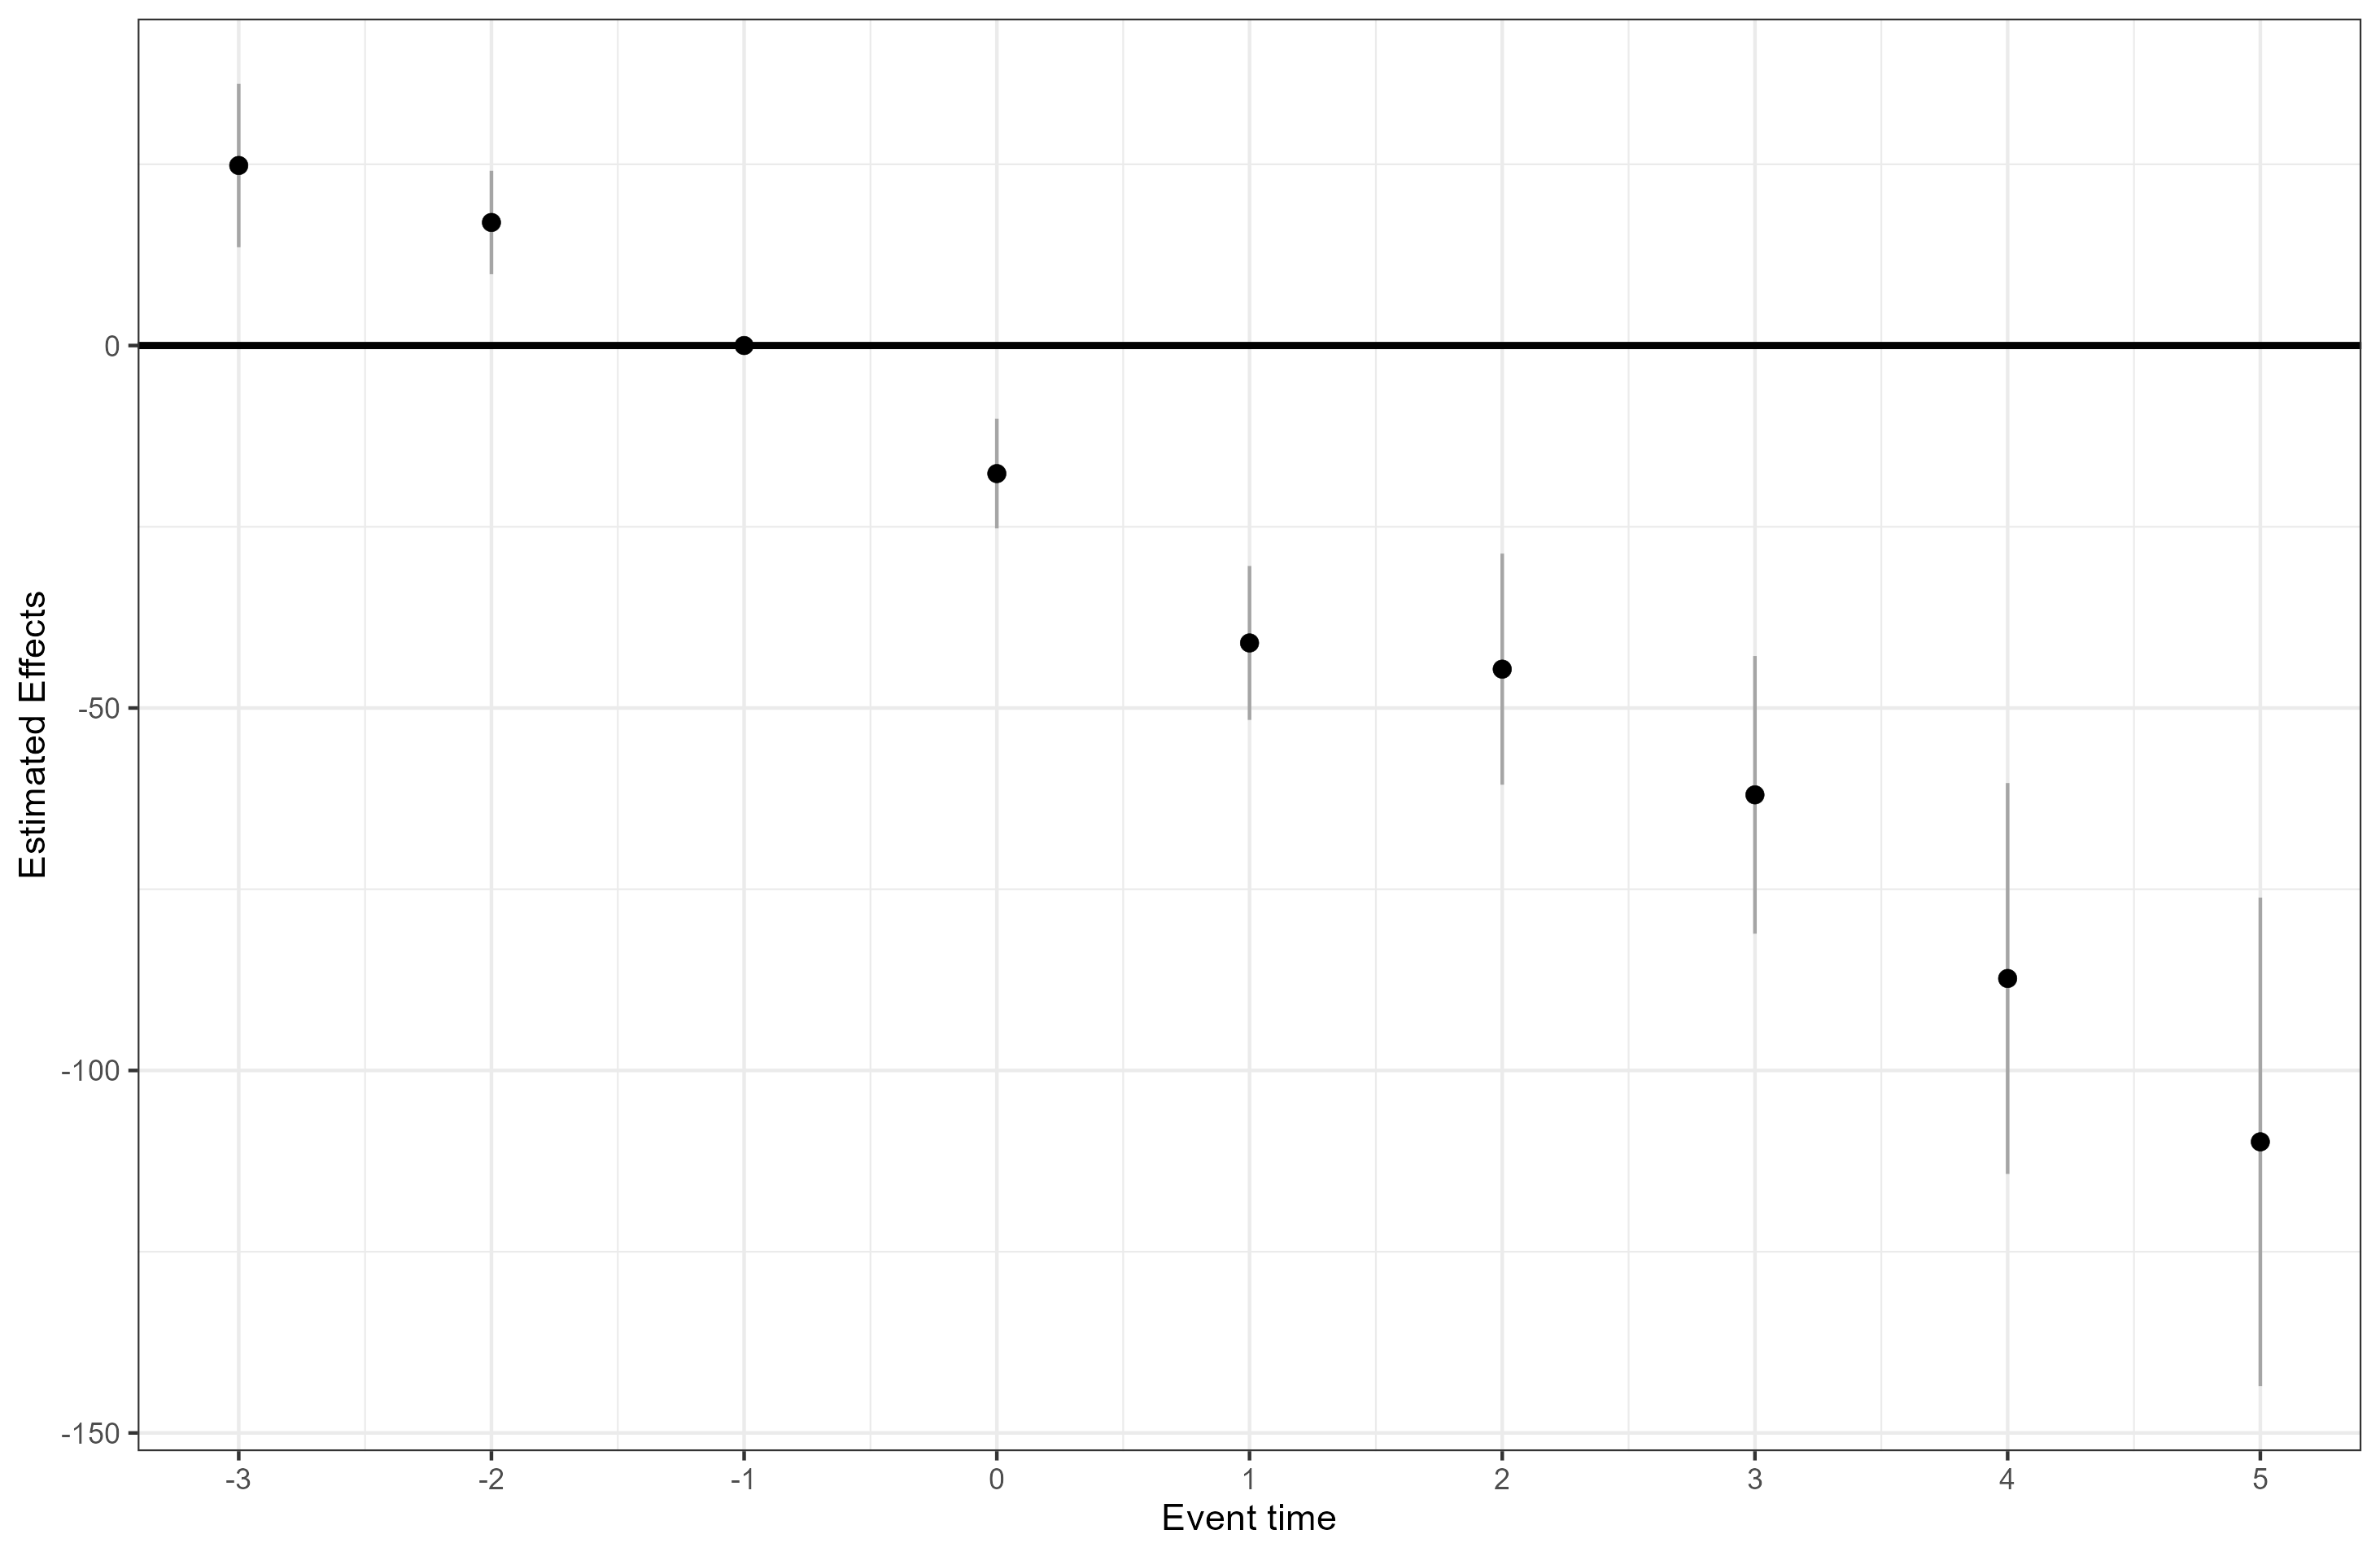
\includegraphics[width=0.48\textwidth]{../results/elig-netpatrev-cs.png} &
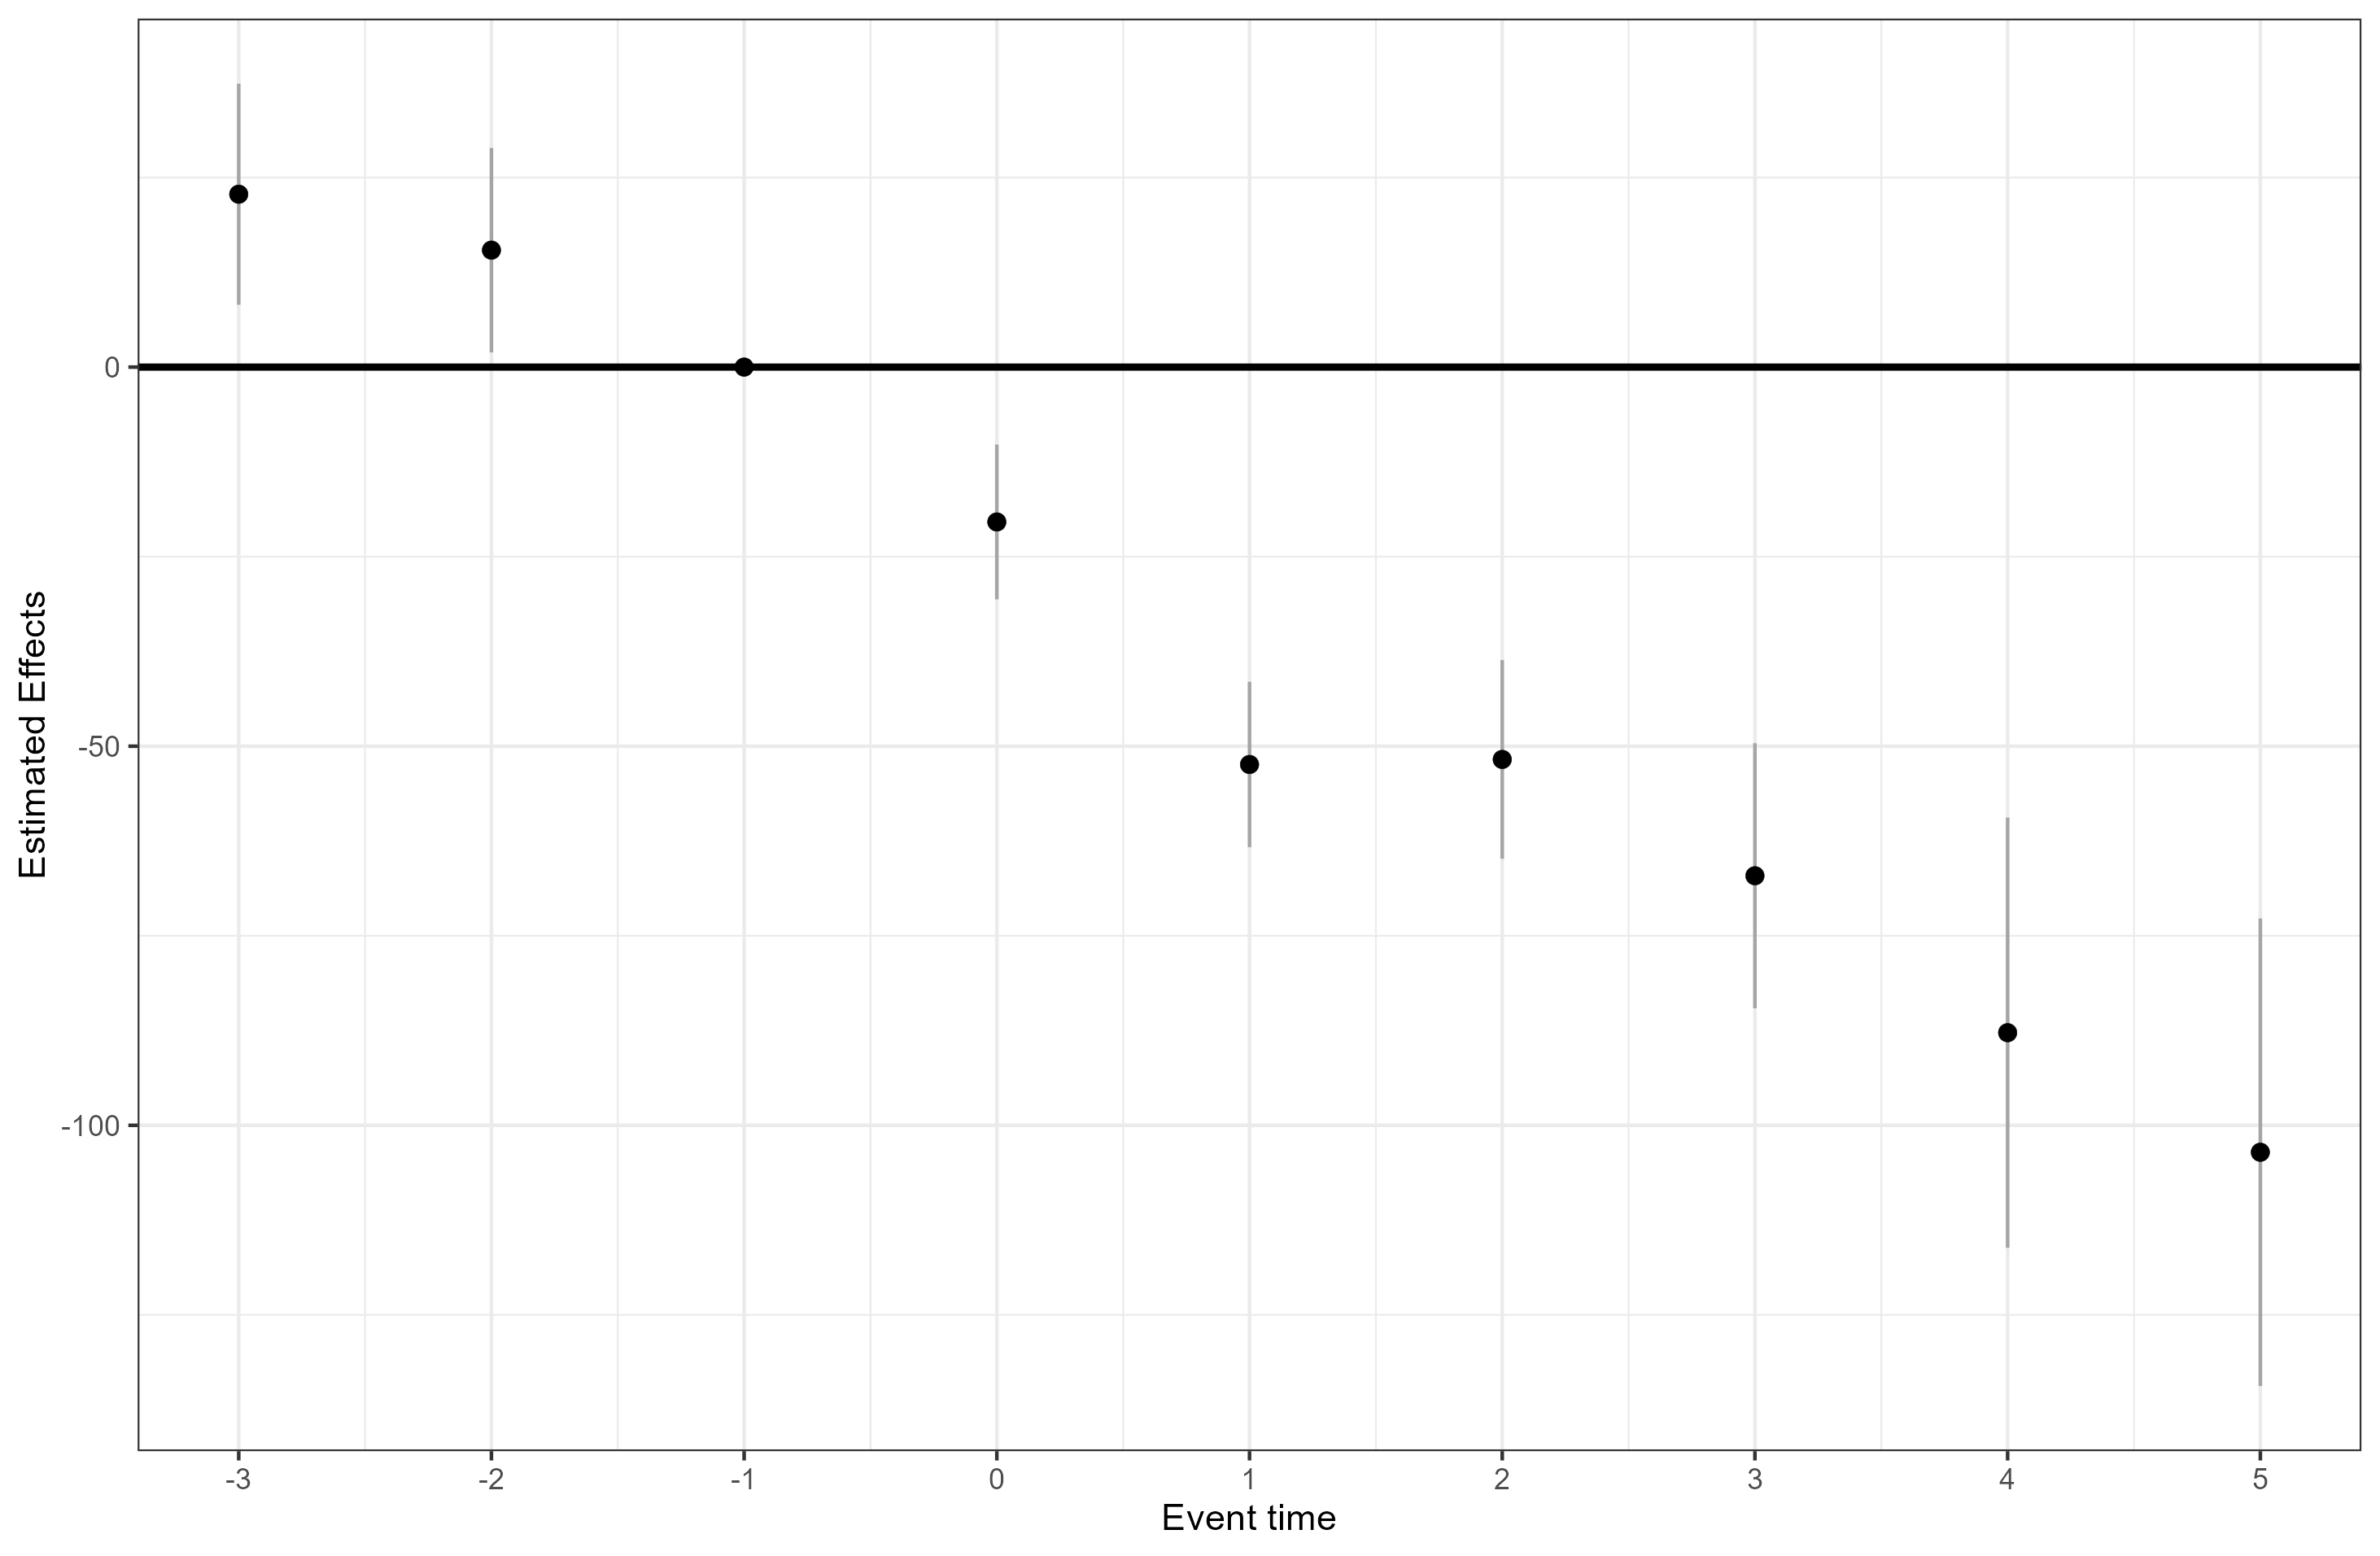
\includegraphics[width=0.48\textwidth]{../results/elig-totopexp-cs.png} \\
\small (c) Net Patient Revenue per Bed & \small (d) Operating Expenses per Bed \\[0.5cm]
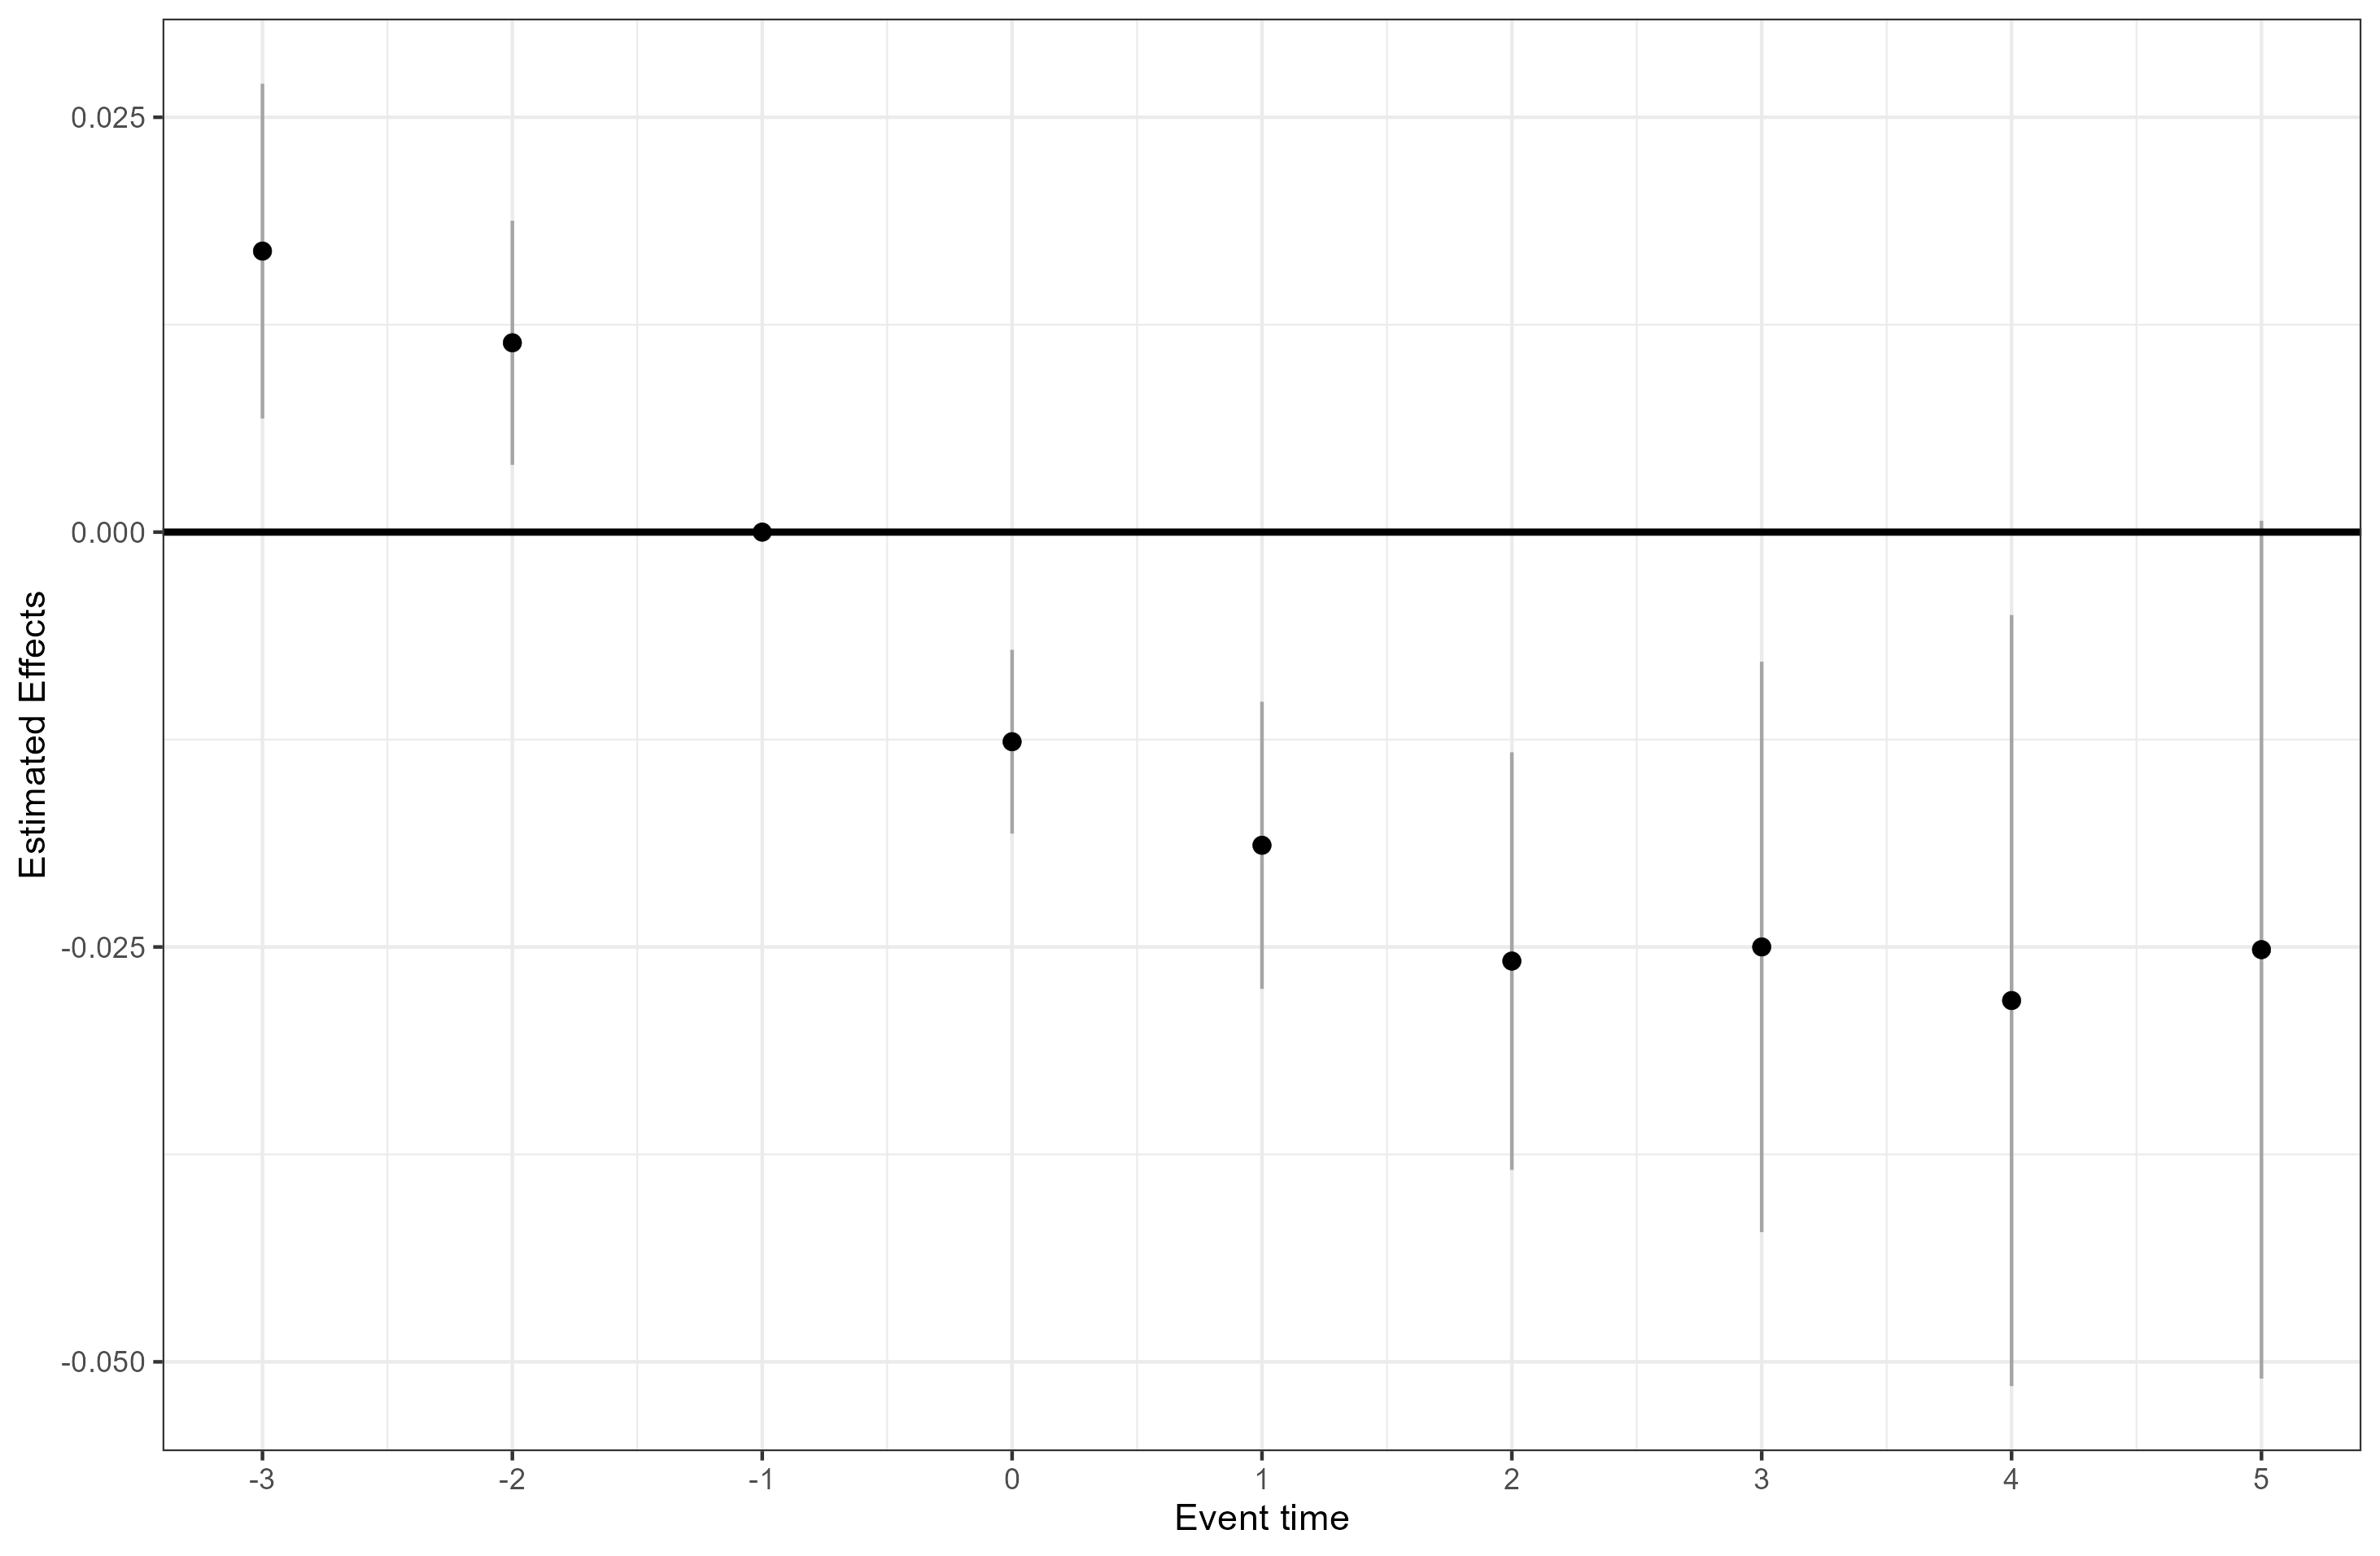
\includegraphics[width=0.48\textwidth]{../results/elig-netfixed-cs.png} &
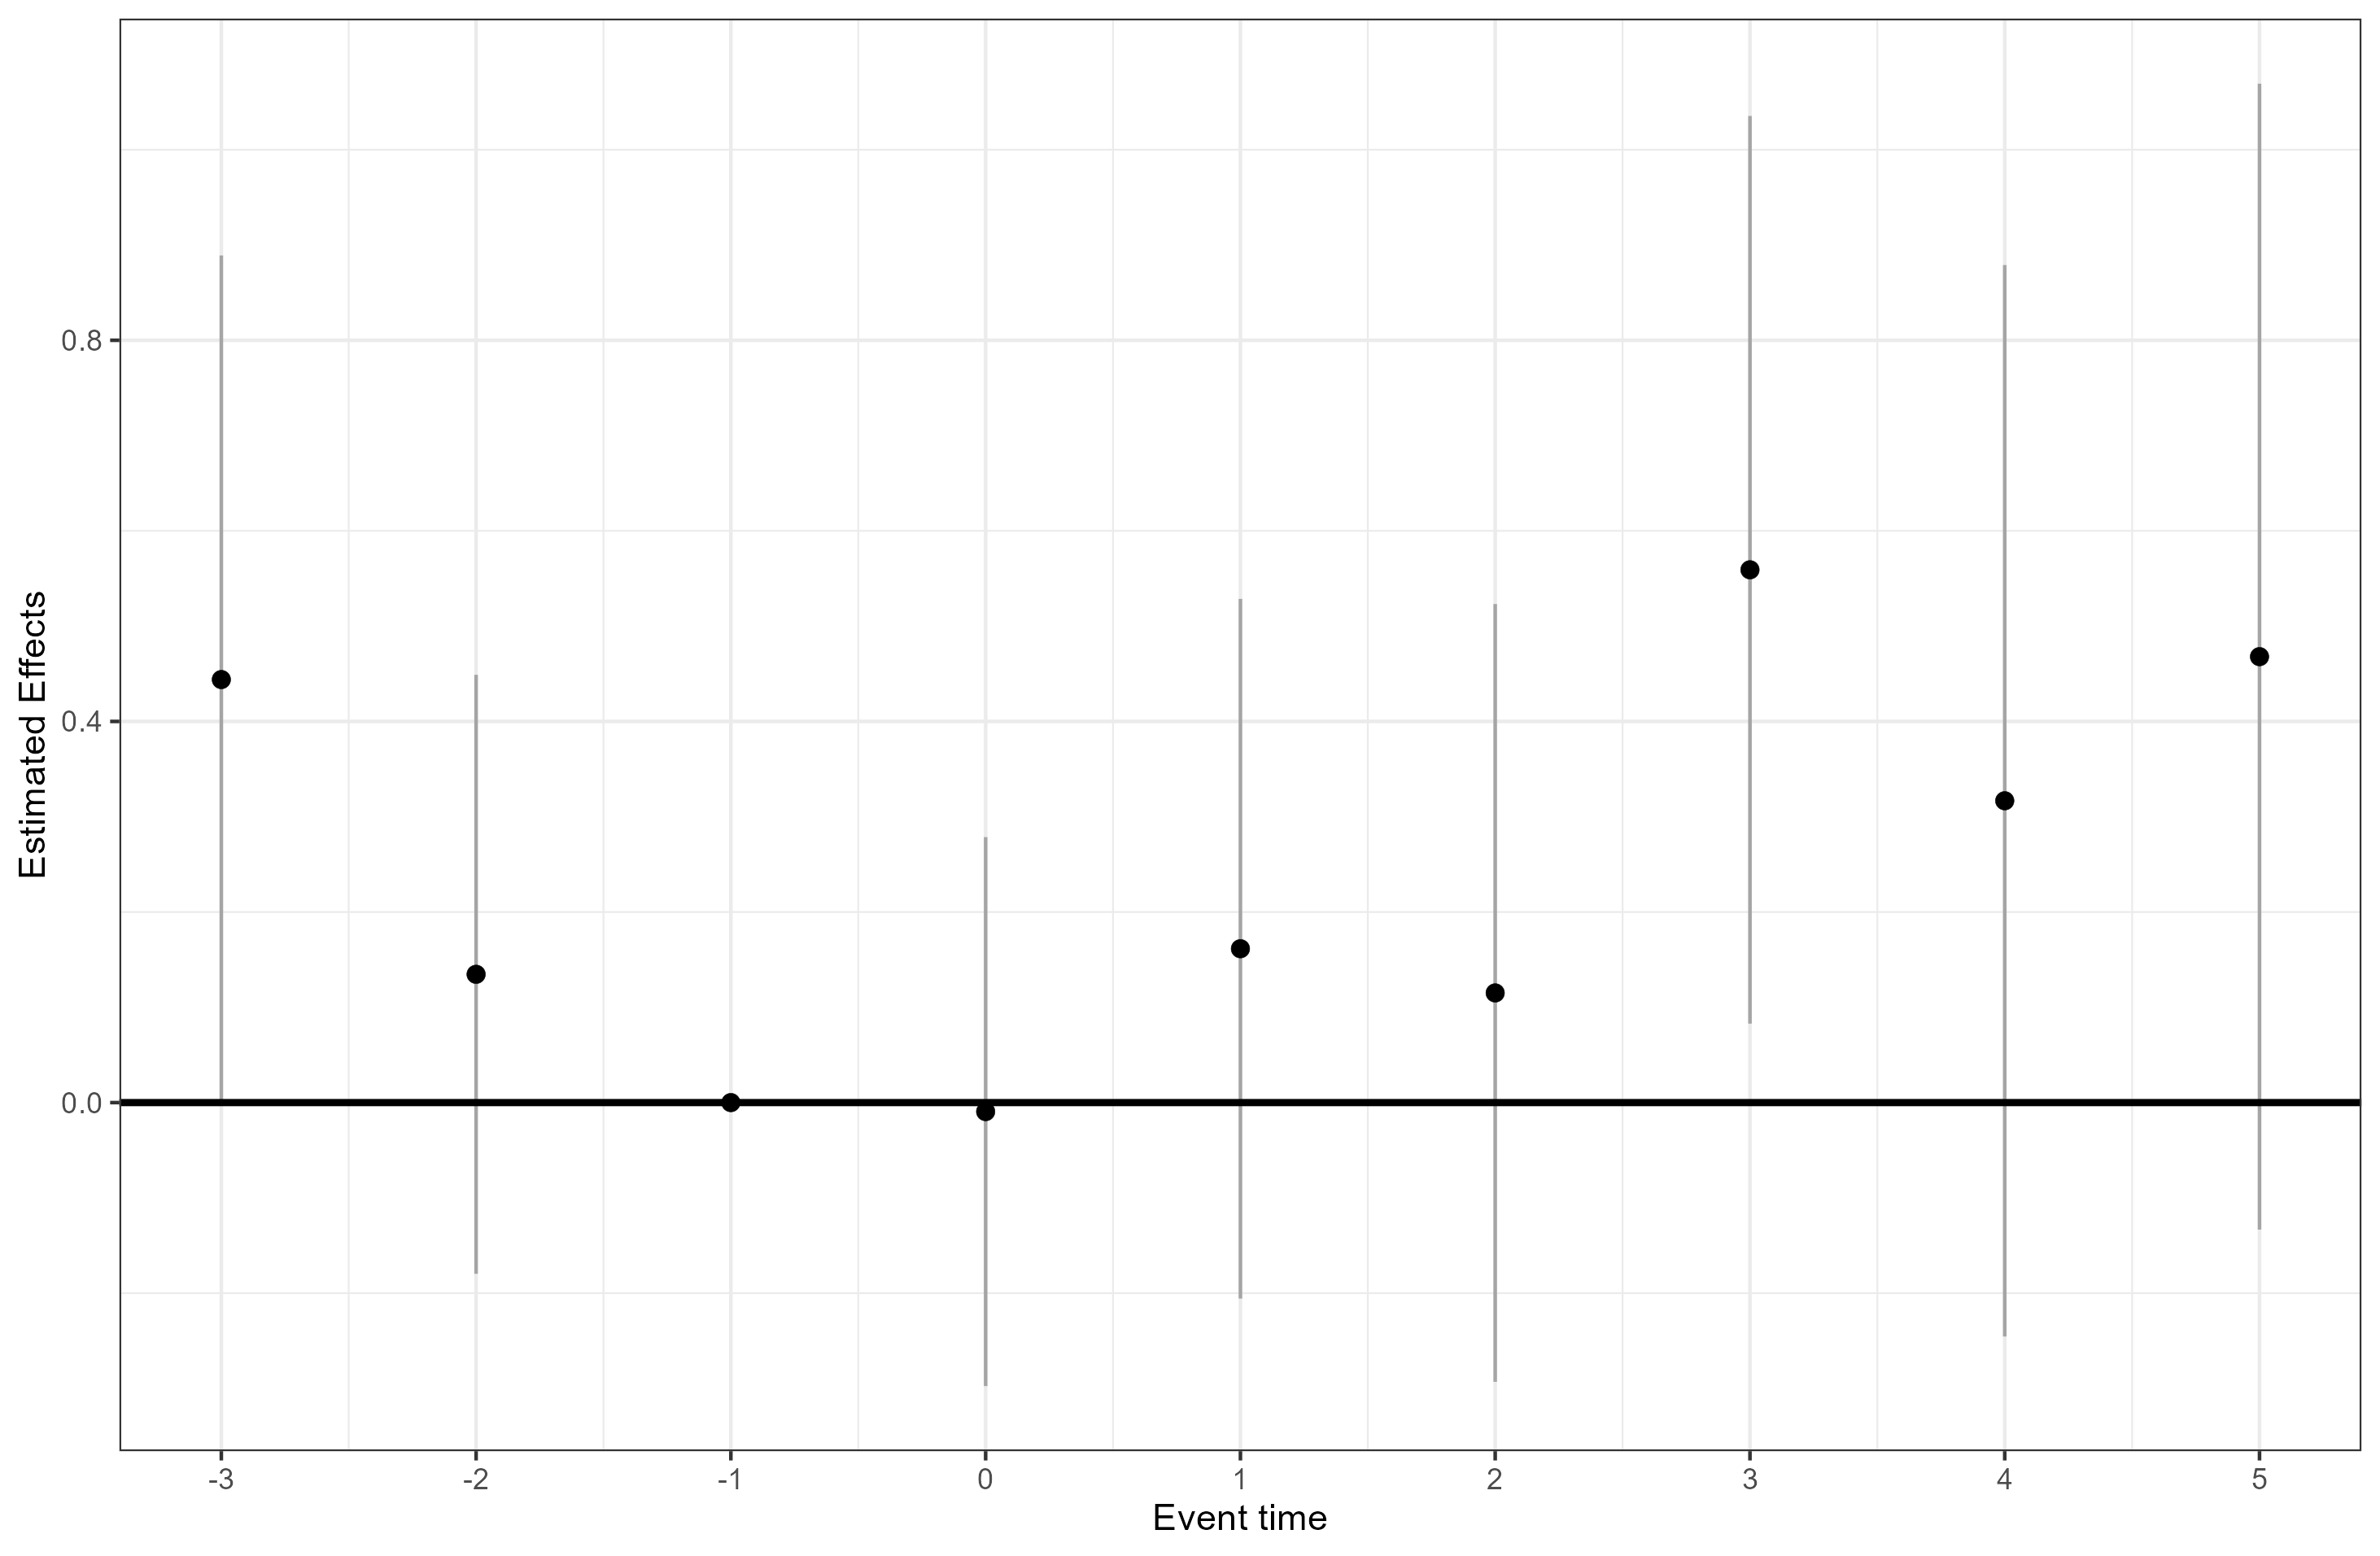
\includegraphics[width=0.48\textwidth]{../results/elig-capex-cs.png} \\
\small (e) Net Fixed Assets & \small (f) Capital Expenditures
\end{tabular}
\end{minipage}
\end{figure}

\clearpage

\begin{figure}[!h]
\centering
\begin{minipage}[h]{6in}
\caption[CS Event Studies (Eligibility): Capacity]{\textbf{CS Event-Study Estimates (Eligibility-Restricted): Capacity, Staffing, and System Membership}\footnote{Callaway--Sant'Anna event-study estimates with 95\% confidence intervals by years relative to designation, eligibility-restricted design (cohorts 1999--2005), not-yet-treated control group, universal base period.}}
\label{fig:elig-cs-capacity}
\begin{tabular}{cc}
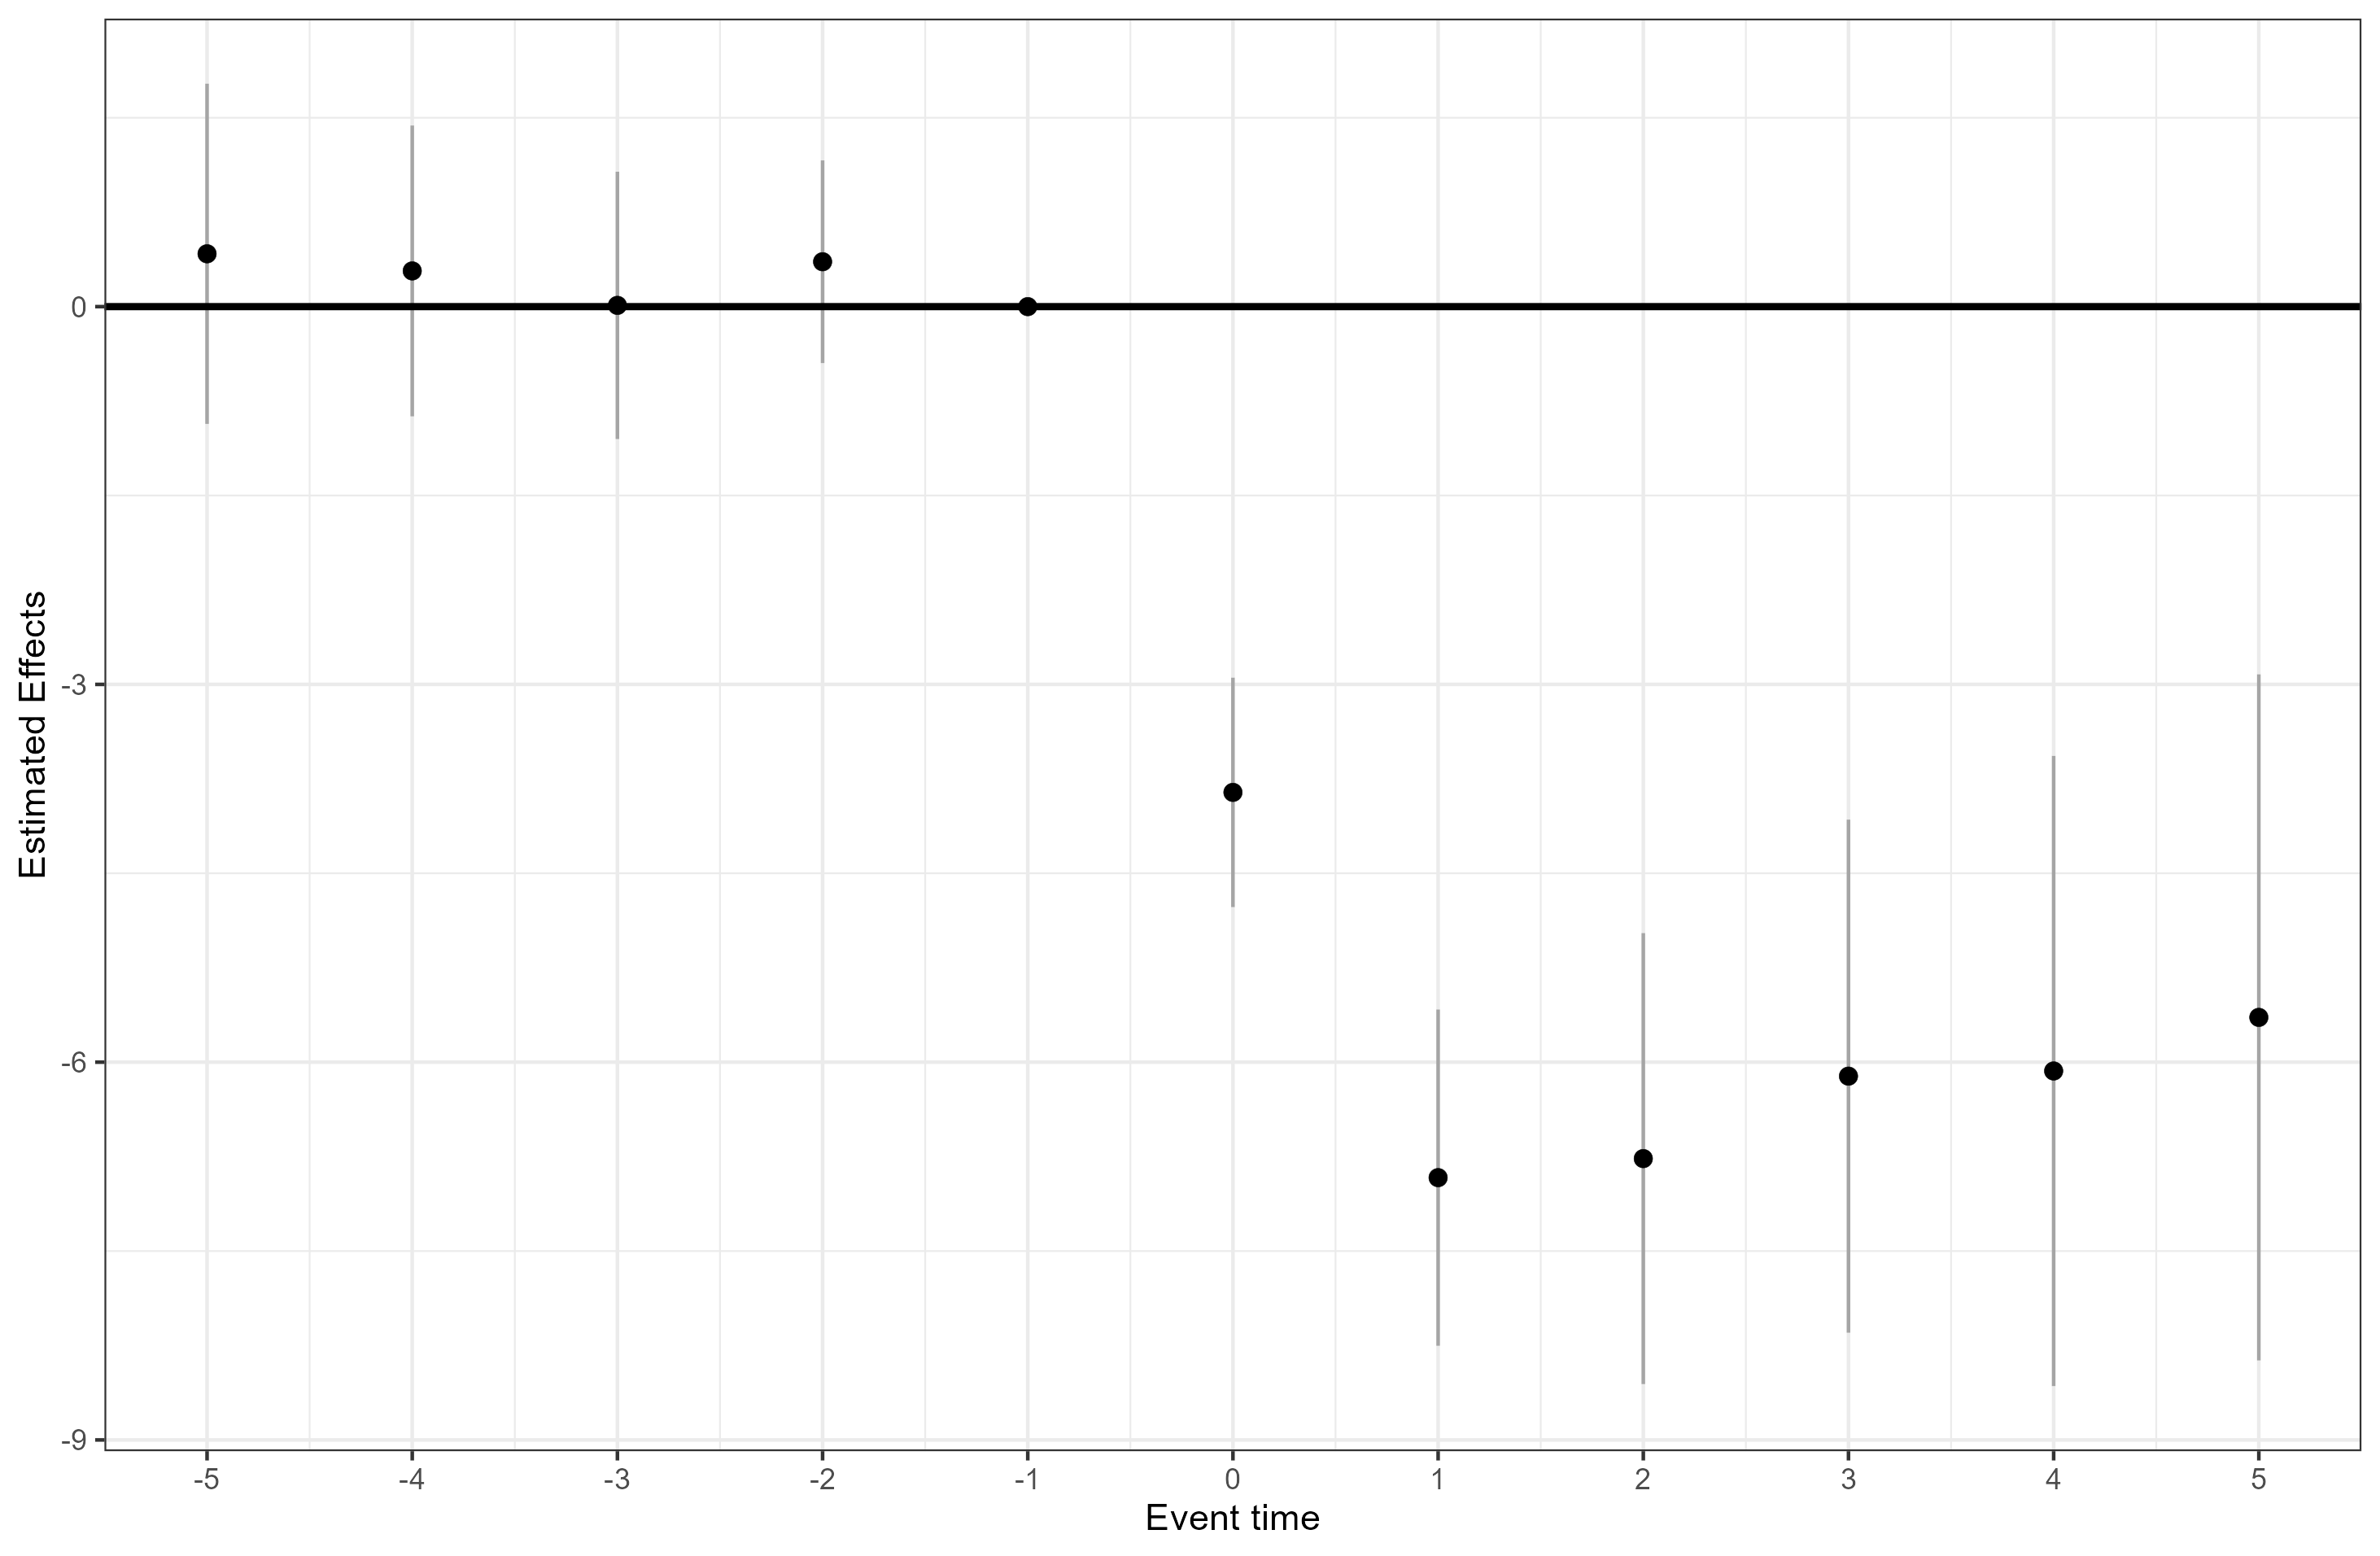
\includegraphics[width=0.48\textwidth]{../results/elig-beds-cs.png} &
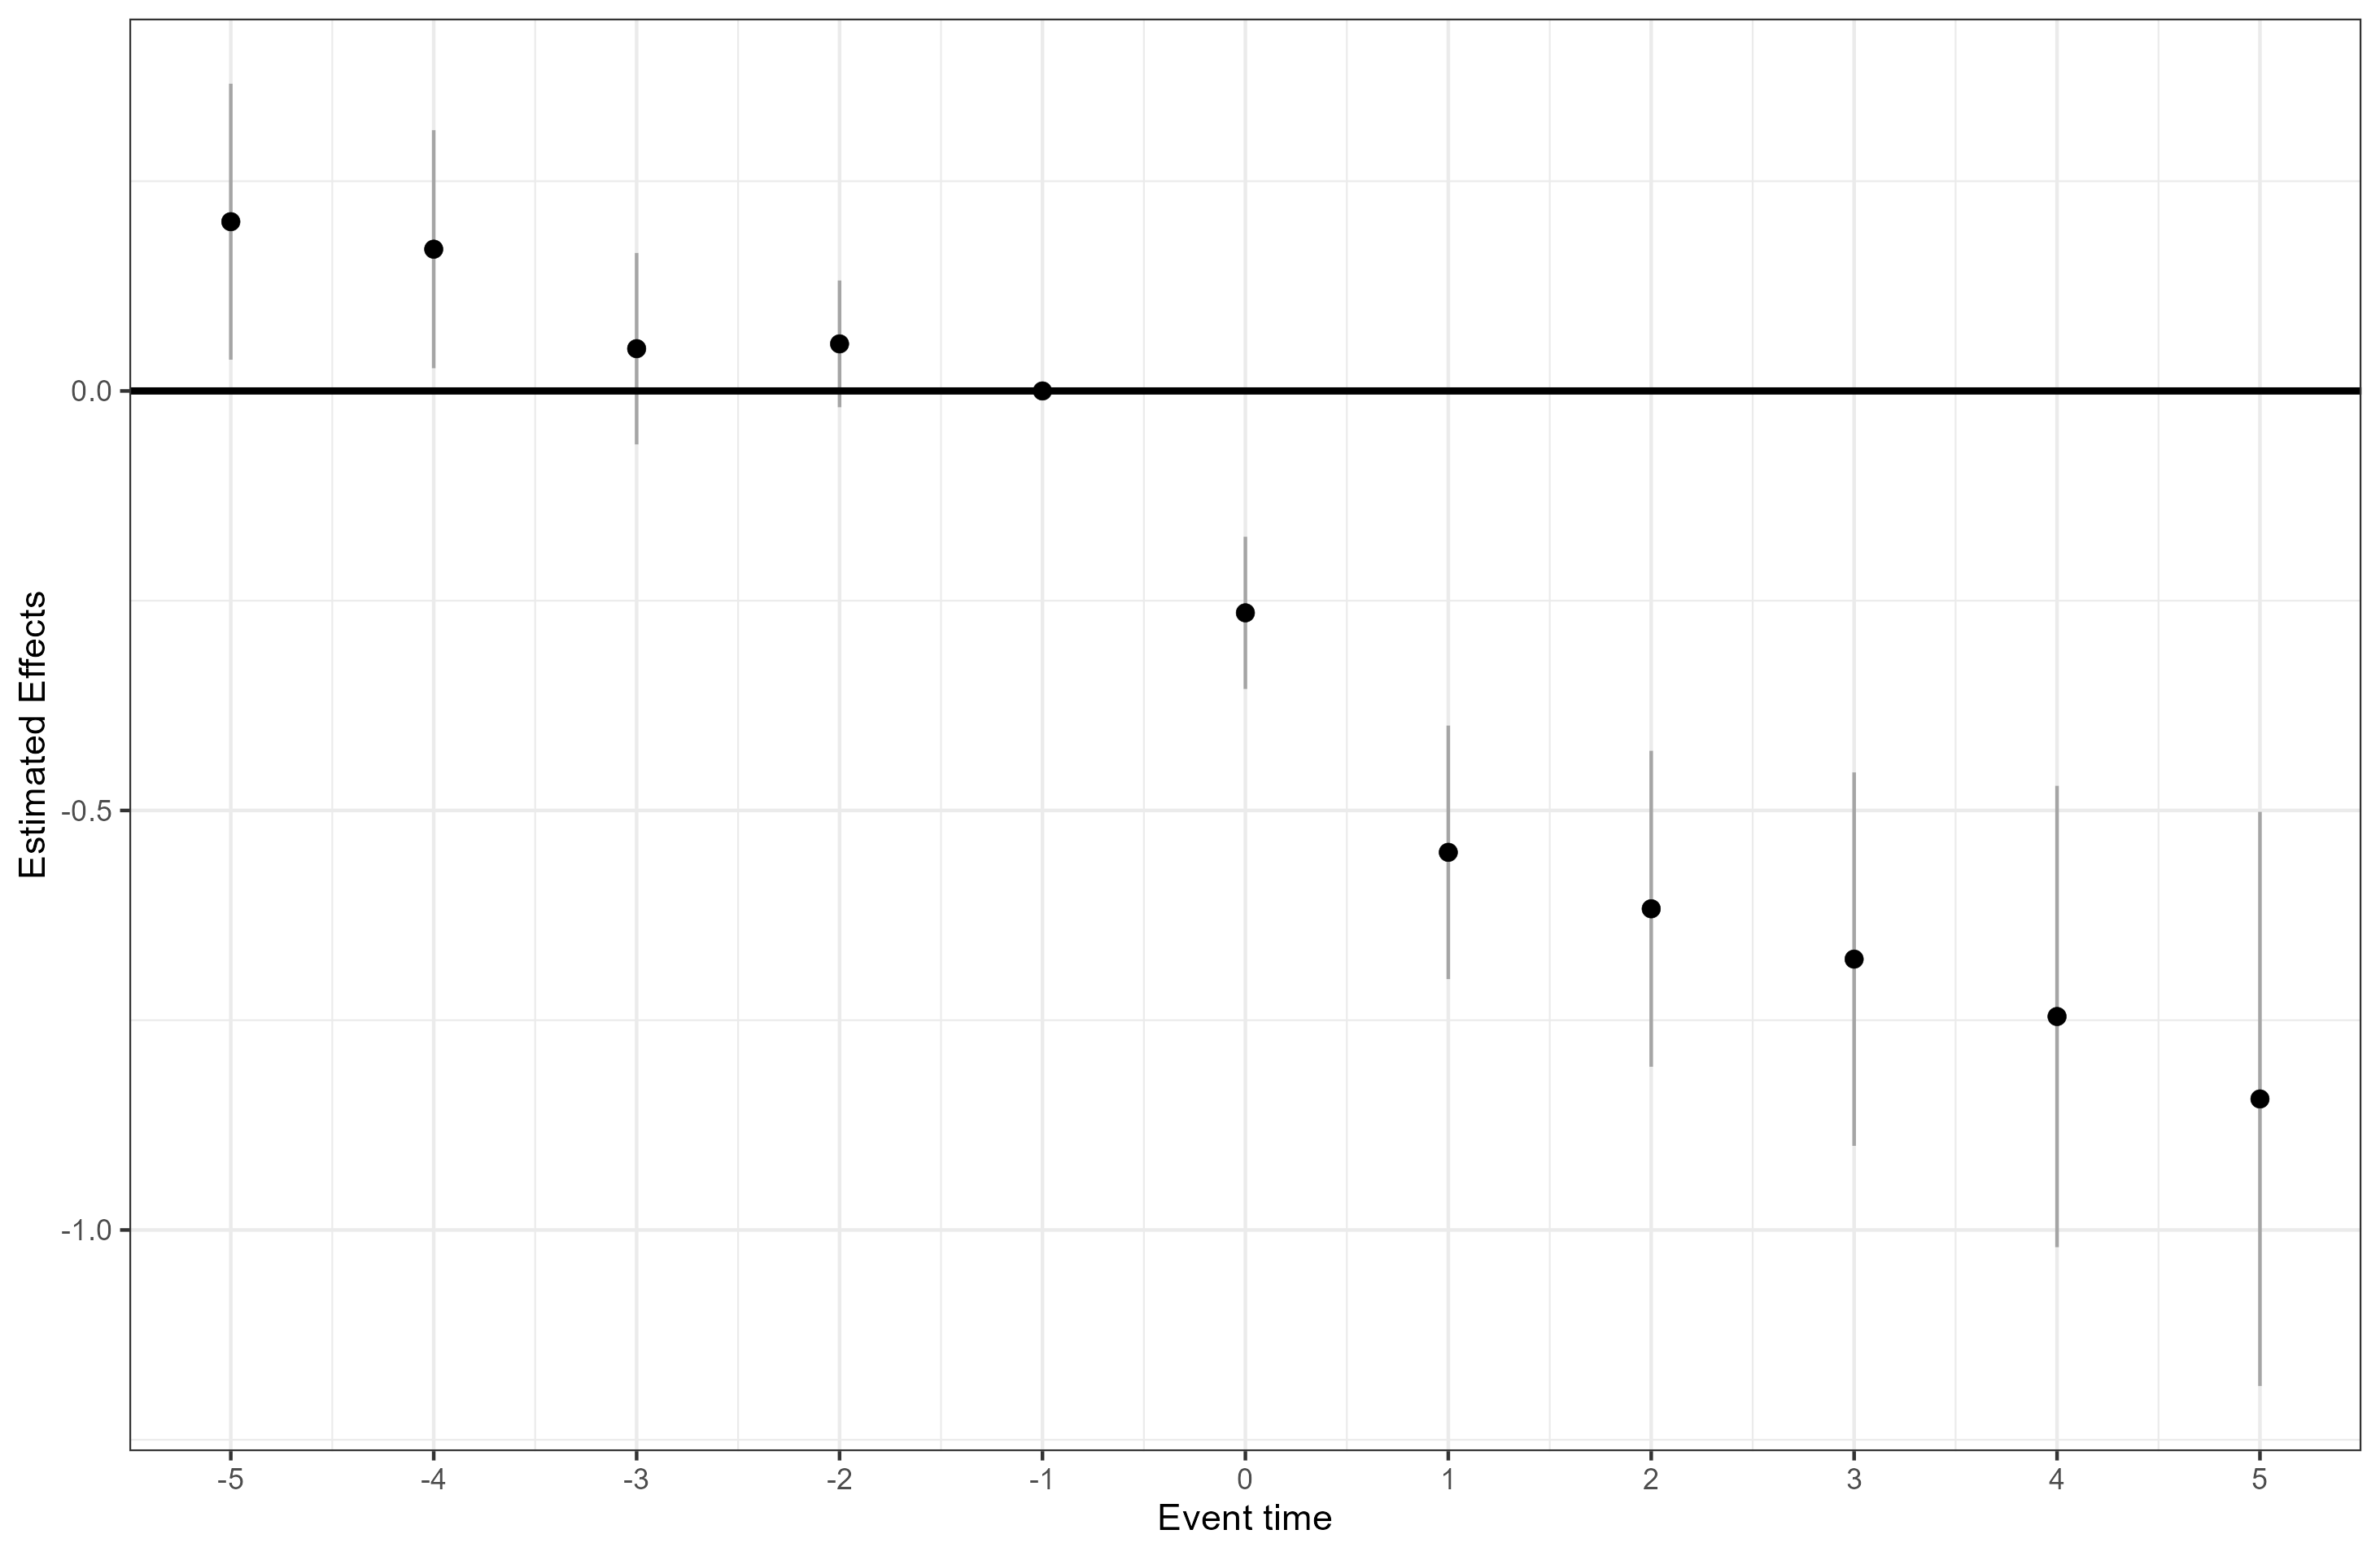
\includegraphics[width=0.48\textwidth]{../results/elig-beds_ob-cs.png} \\
\small (a) Total Beds & \small (b) Obstetric Beds \\[0.5cm]
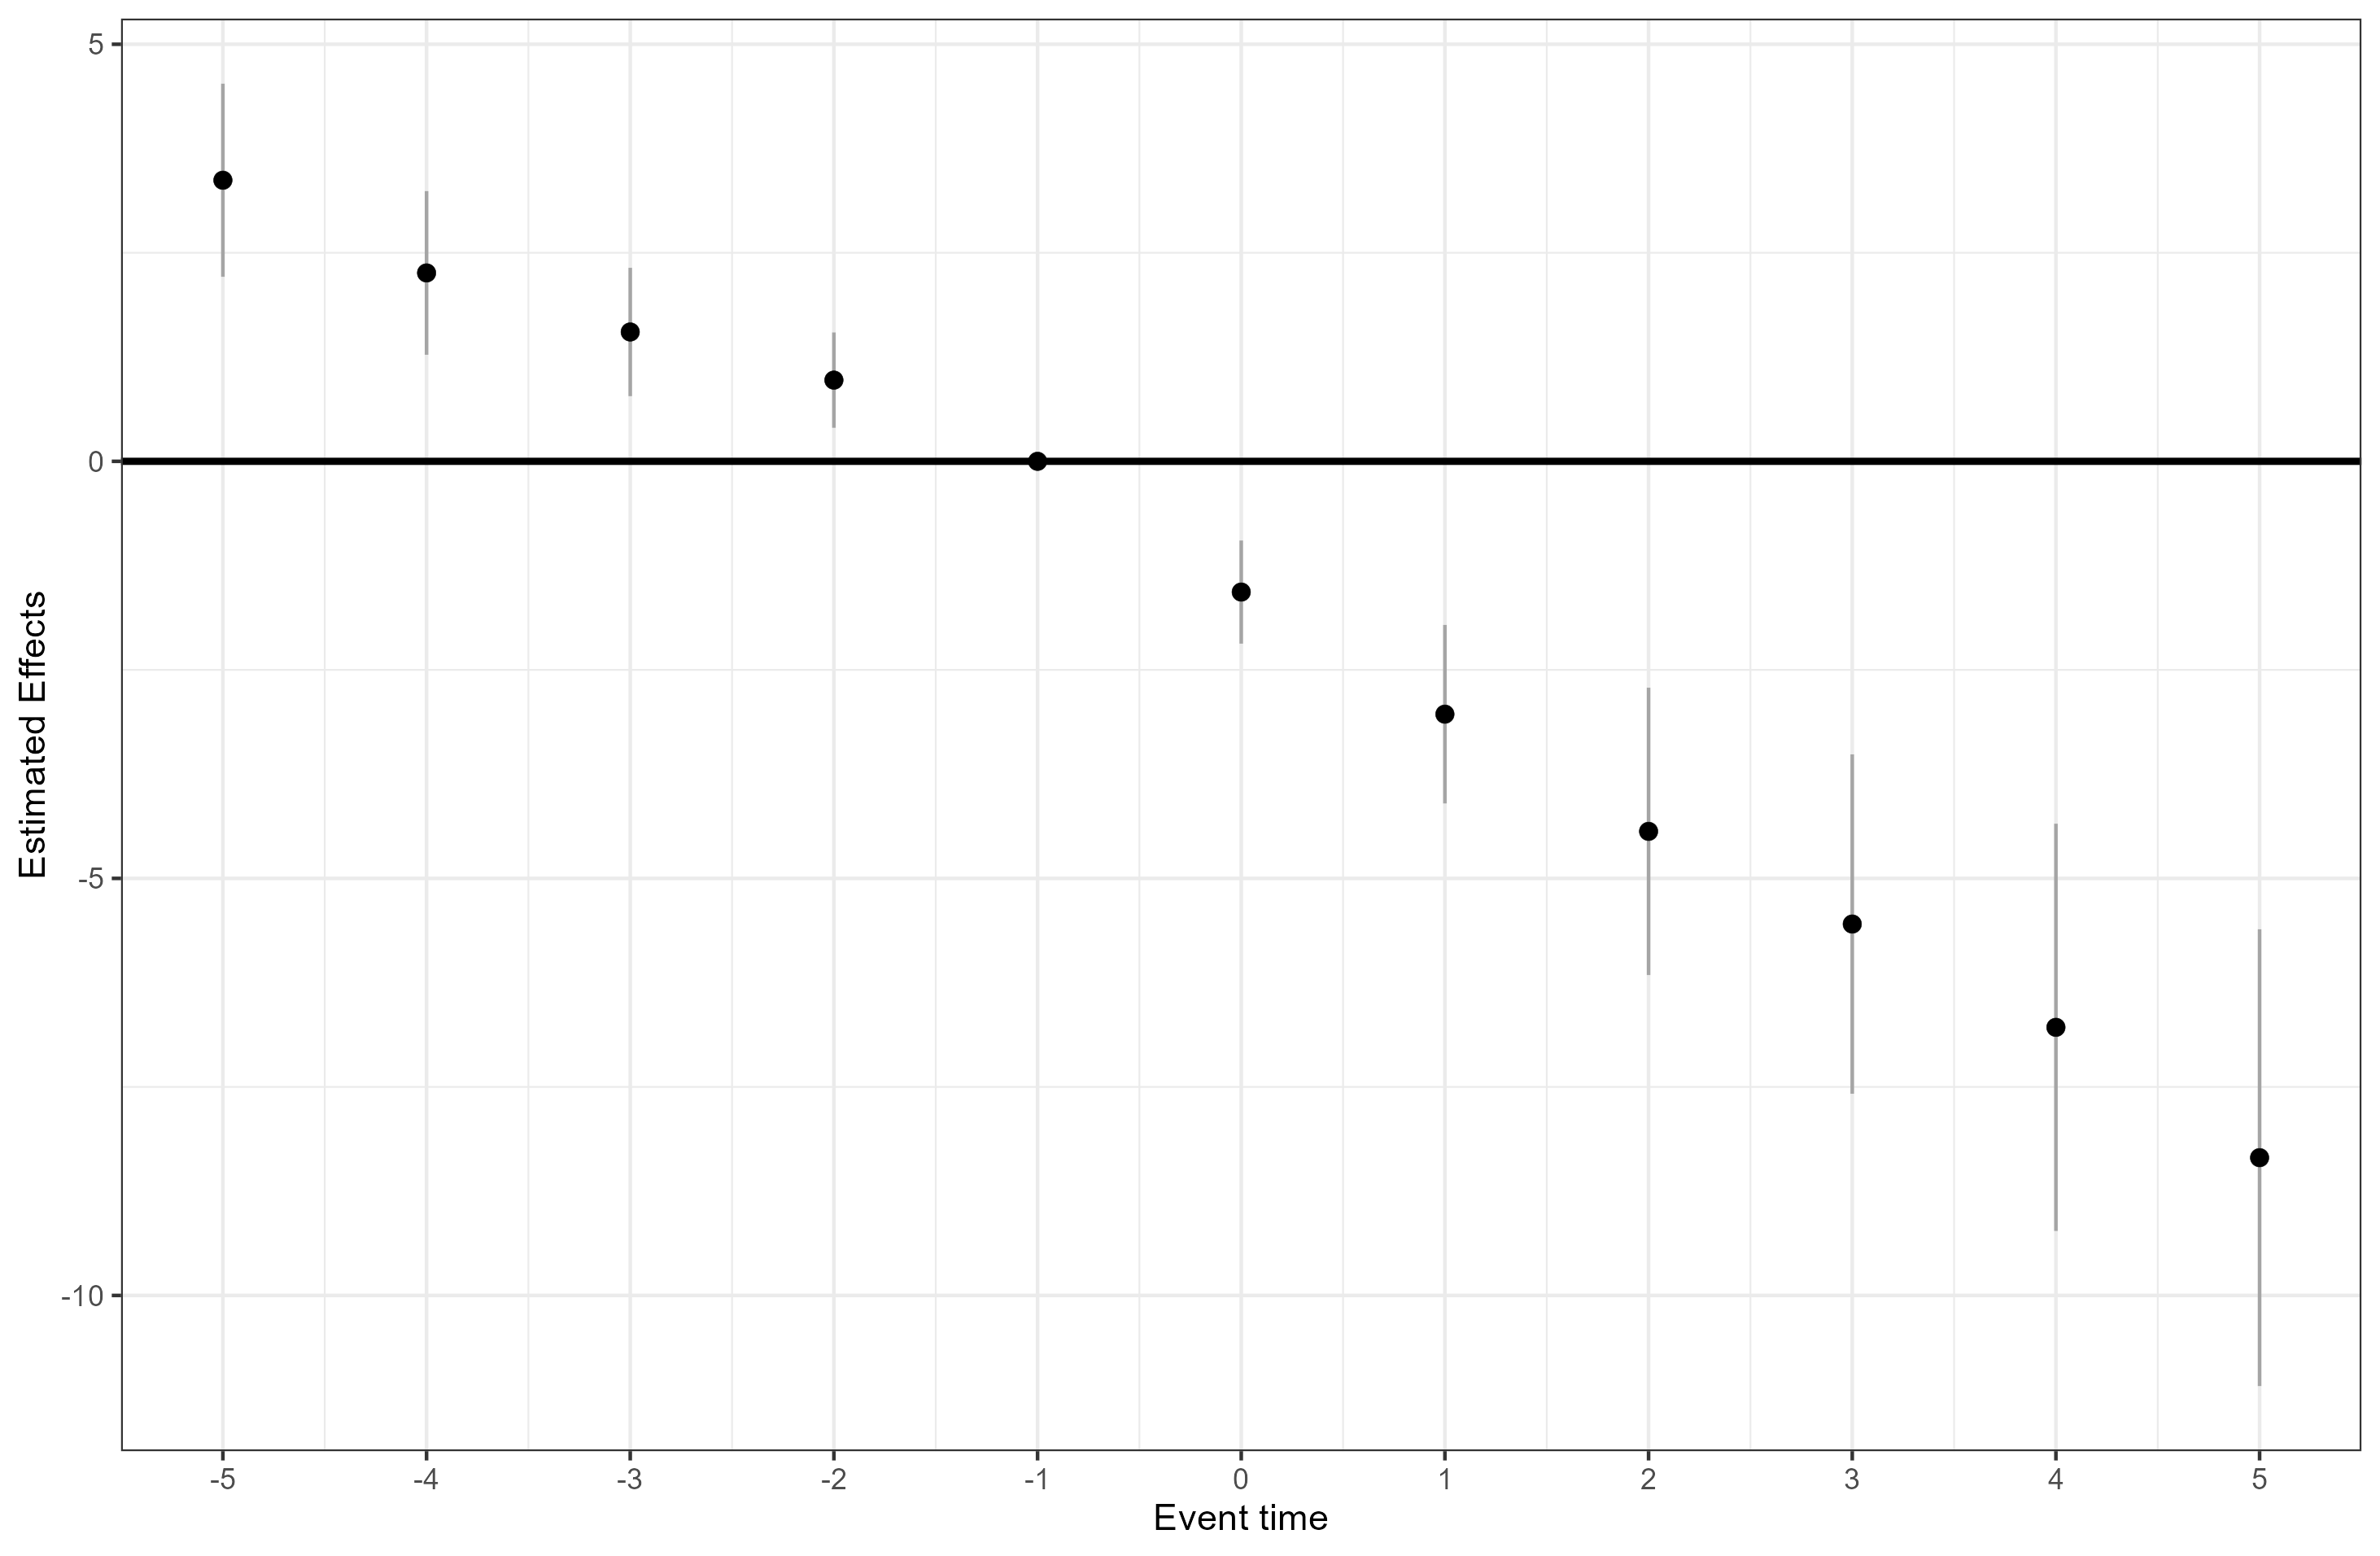
\includegraphics[width=0.48\textwidth]{../results/elig-ftern-cs.png} &
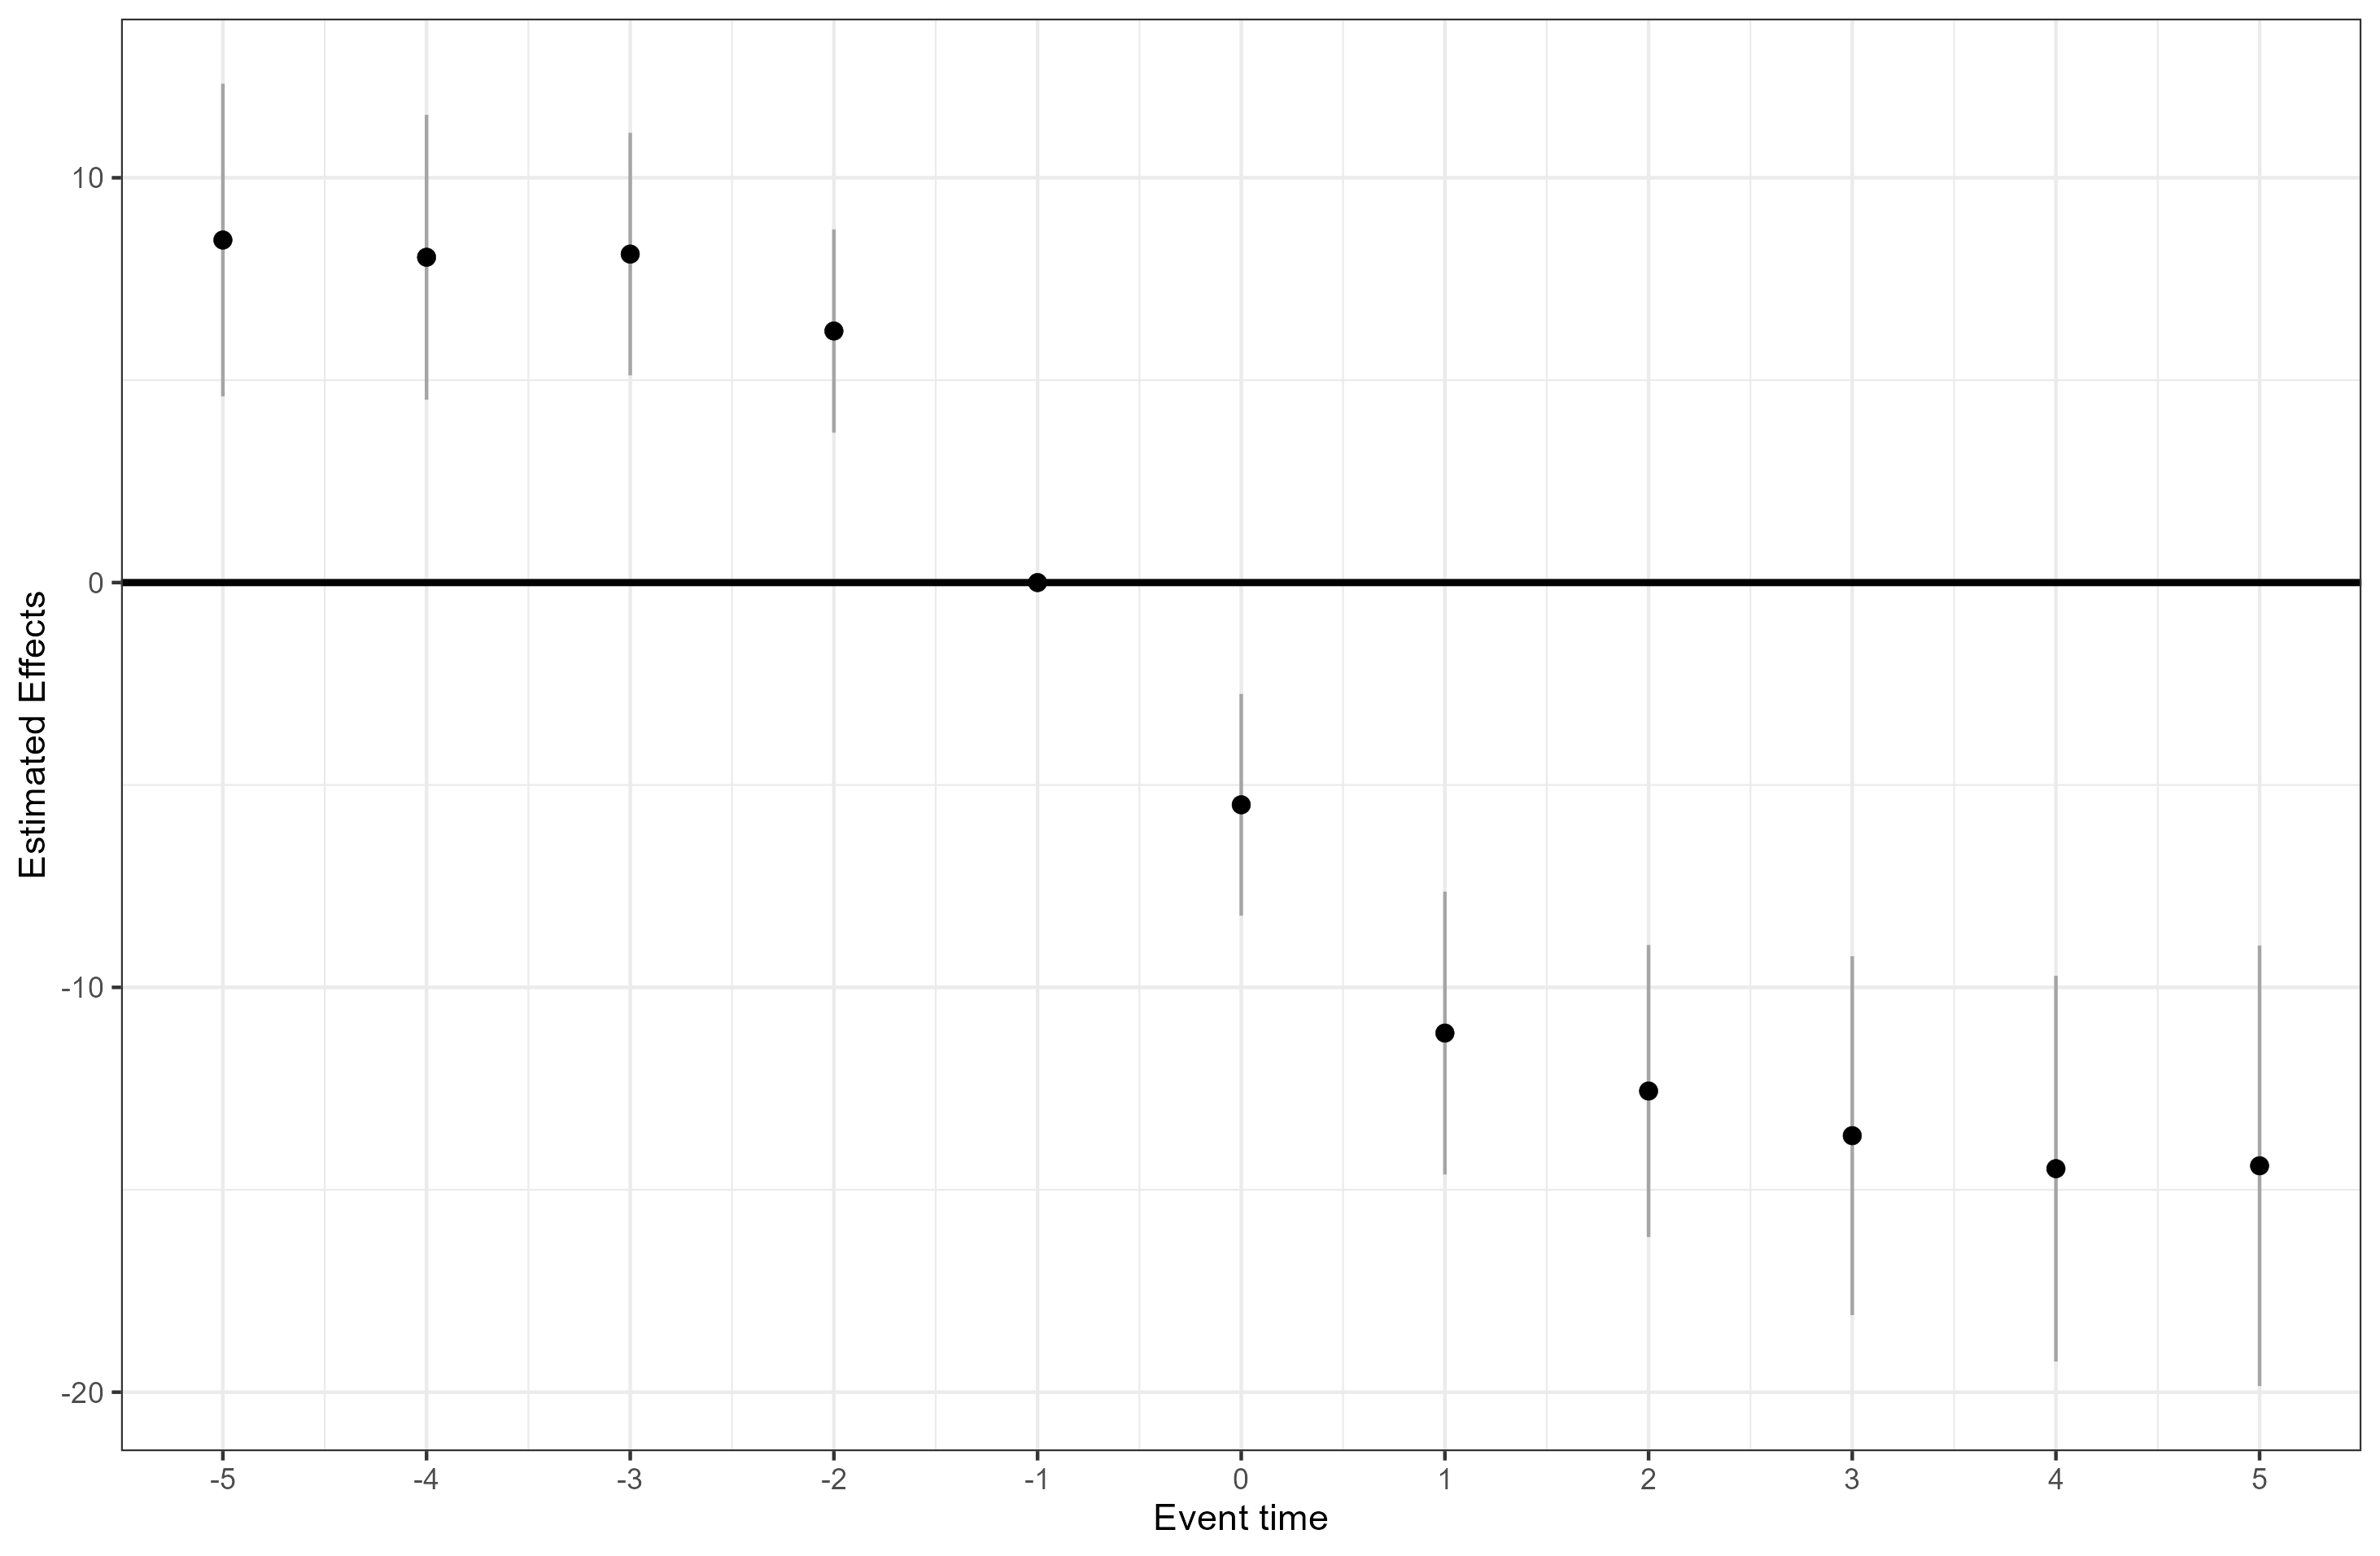
\includegraphics[width=0.48\textwidth]{../results/elig-ipdays-cs.png} \\
\small (c) Full Time Equivalent RNs & \small (d) Inpatient Days per Bed \\[0.5cm]
\multicolumn{2}{c}{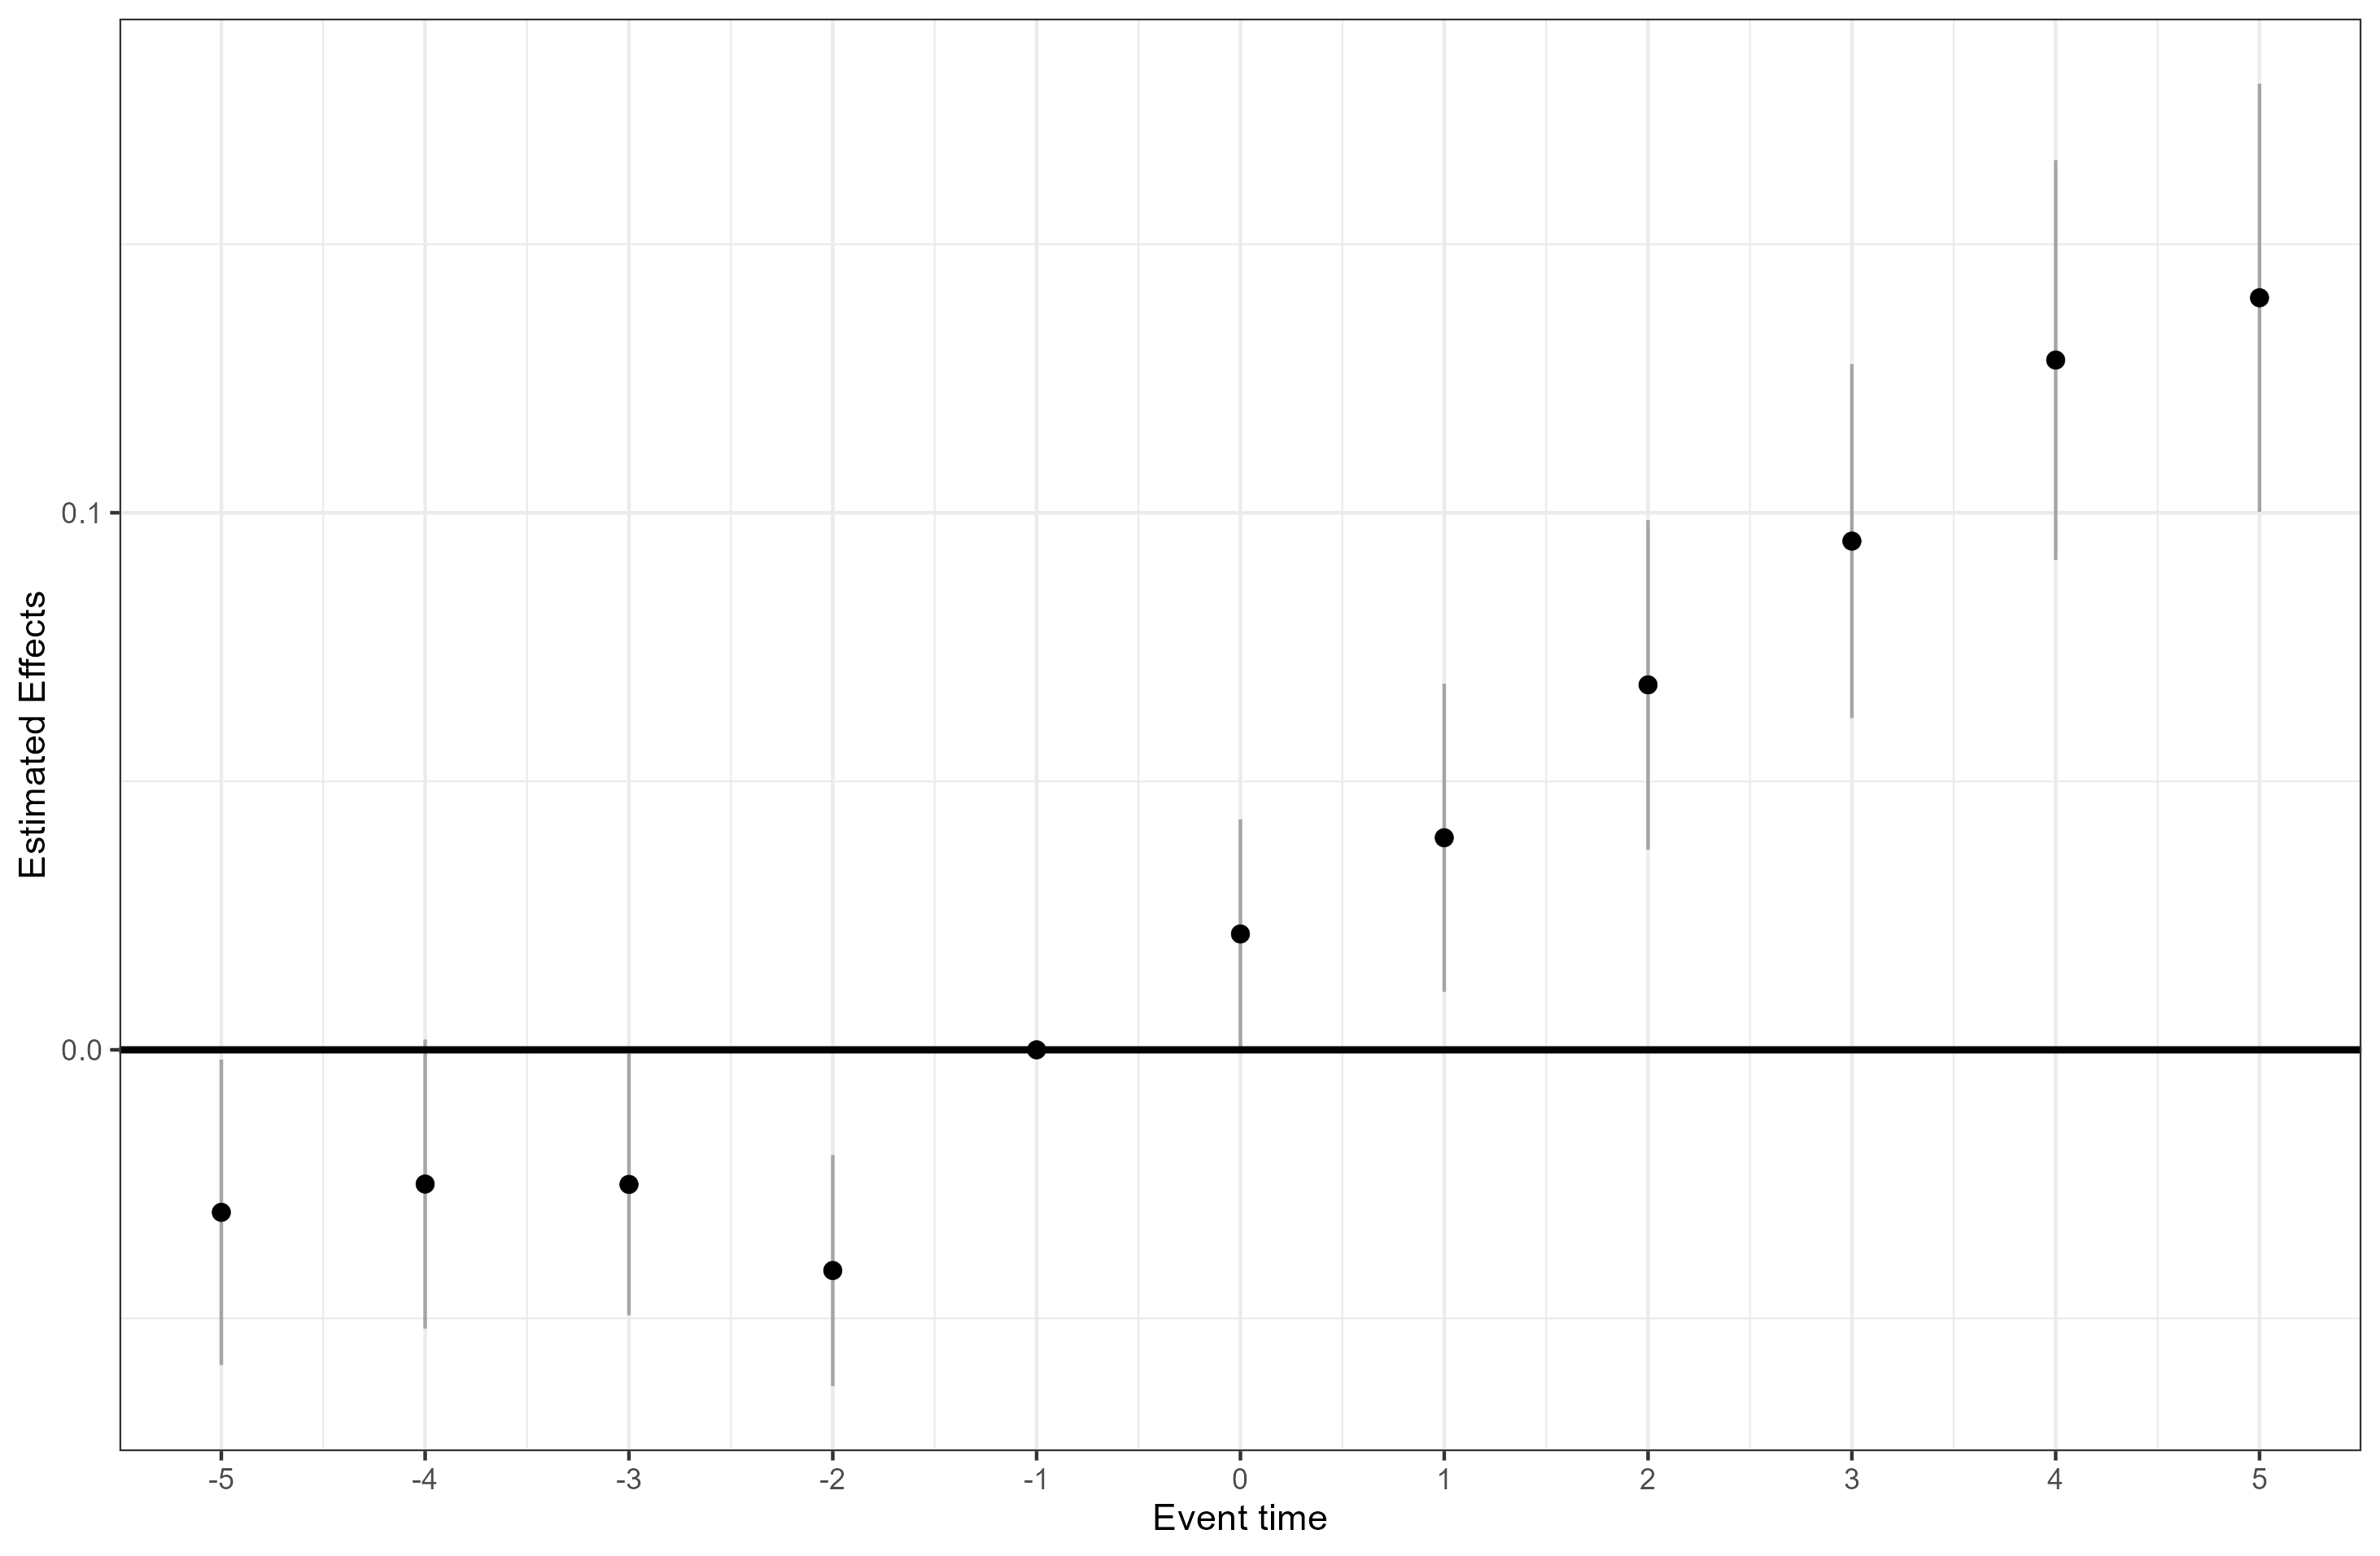
\includegraphics[width=0.48\textwidth]{../results/elig-system-cs.png}} \\
\multicolumn{2}{c}{\small (e) System Membership}
\end{tabular}
\end{minipage}
\end{figure}

\clearpage

\begin{figure}[!h]
\centering
\begin{minipage}[h]{6in}
\caption[Eligibility-Restricted CS Event Studies: Visits and Births]{\textbf{Eligibility-Restricted CS Event-Study Estimates: Outpatient Visits, Emergency Department Visits, and Births}\footnote{Callaway--Sant'Anna event-study estimates with 95\% confidence intervals by years relative to designation, eligibility-restricted design (cohorts 1999--2005), not-yet-treated control group, universal base period. Visit outcomes are annual counts per pre-designation bed; births are annual counts.}}
\label{fig:elig-cs-visits}
\begin{tabular}{cc}
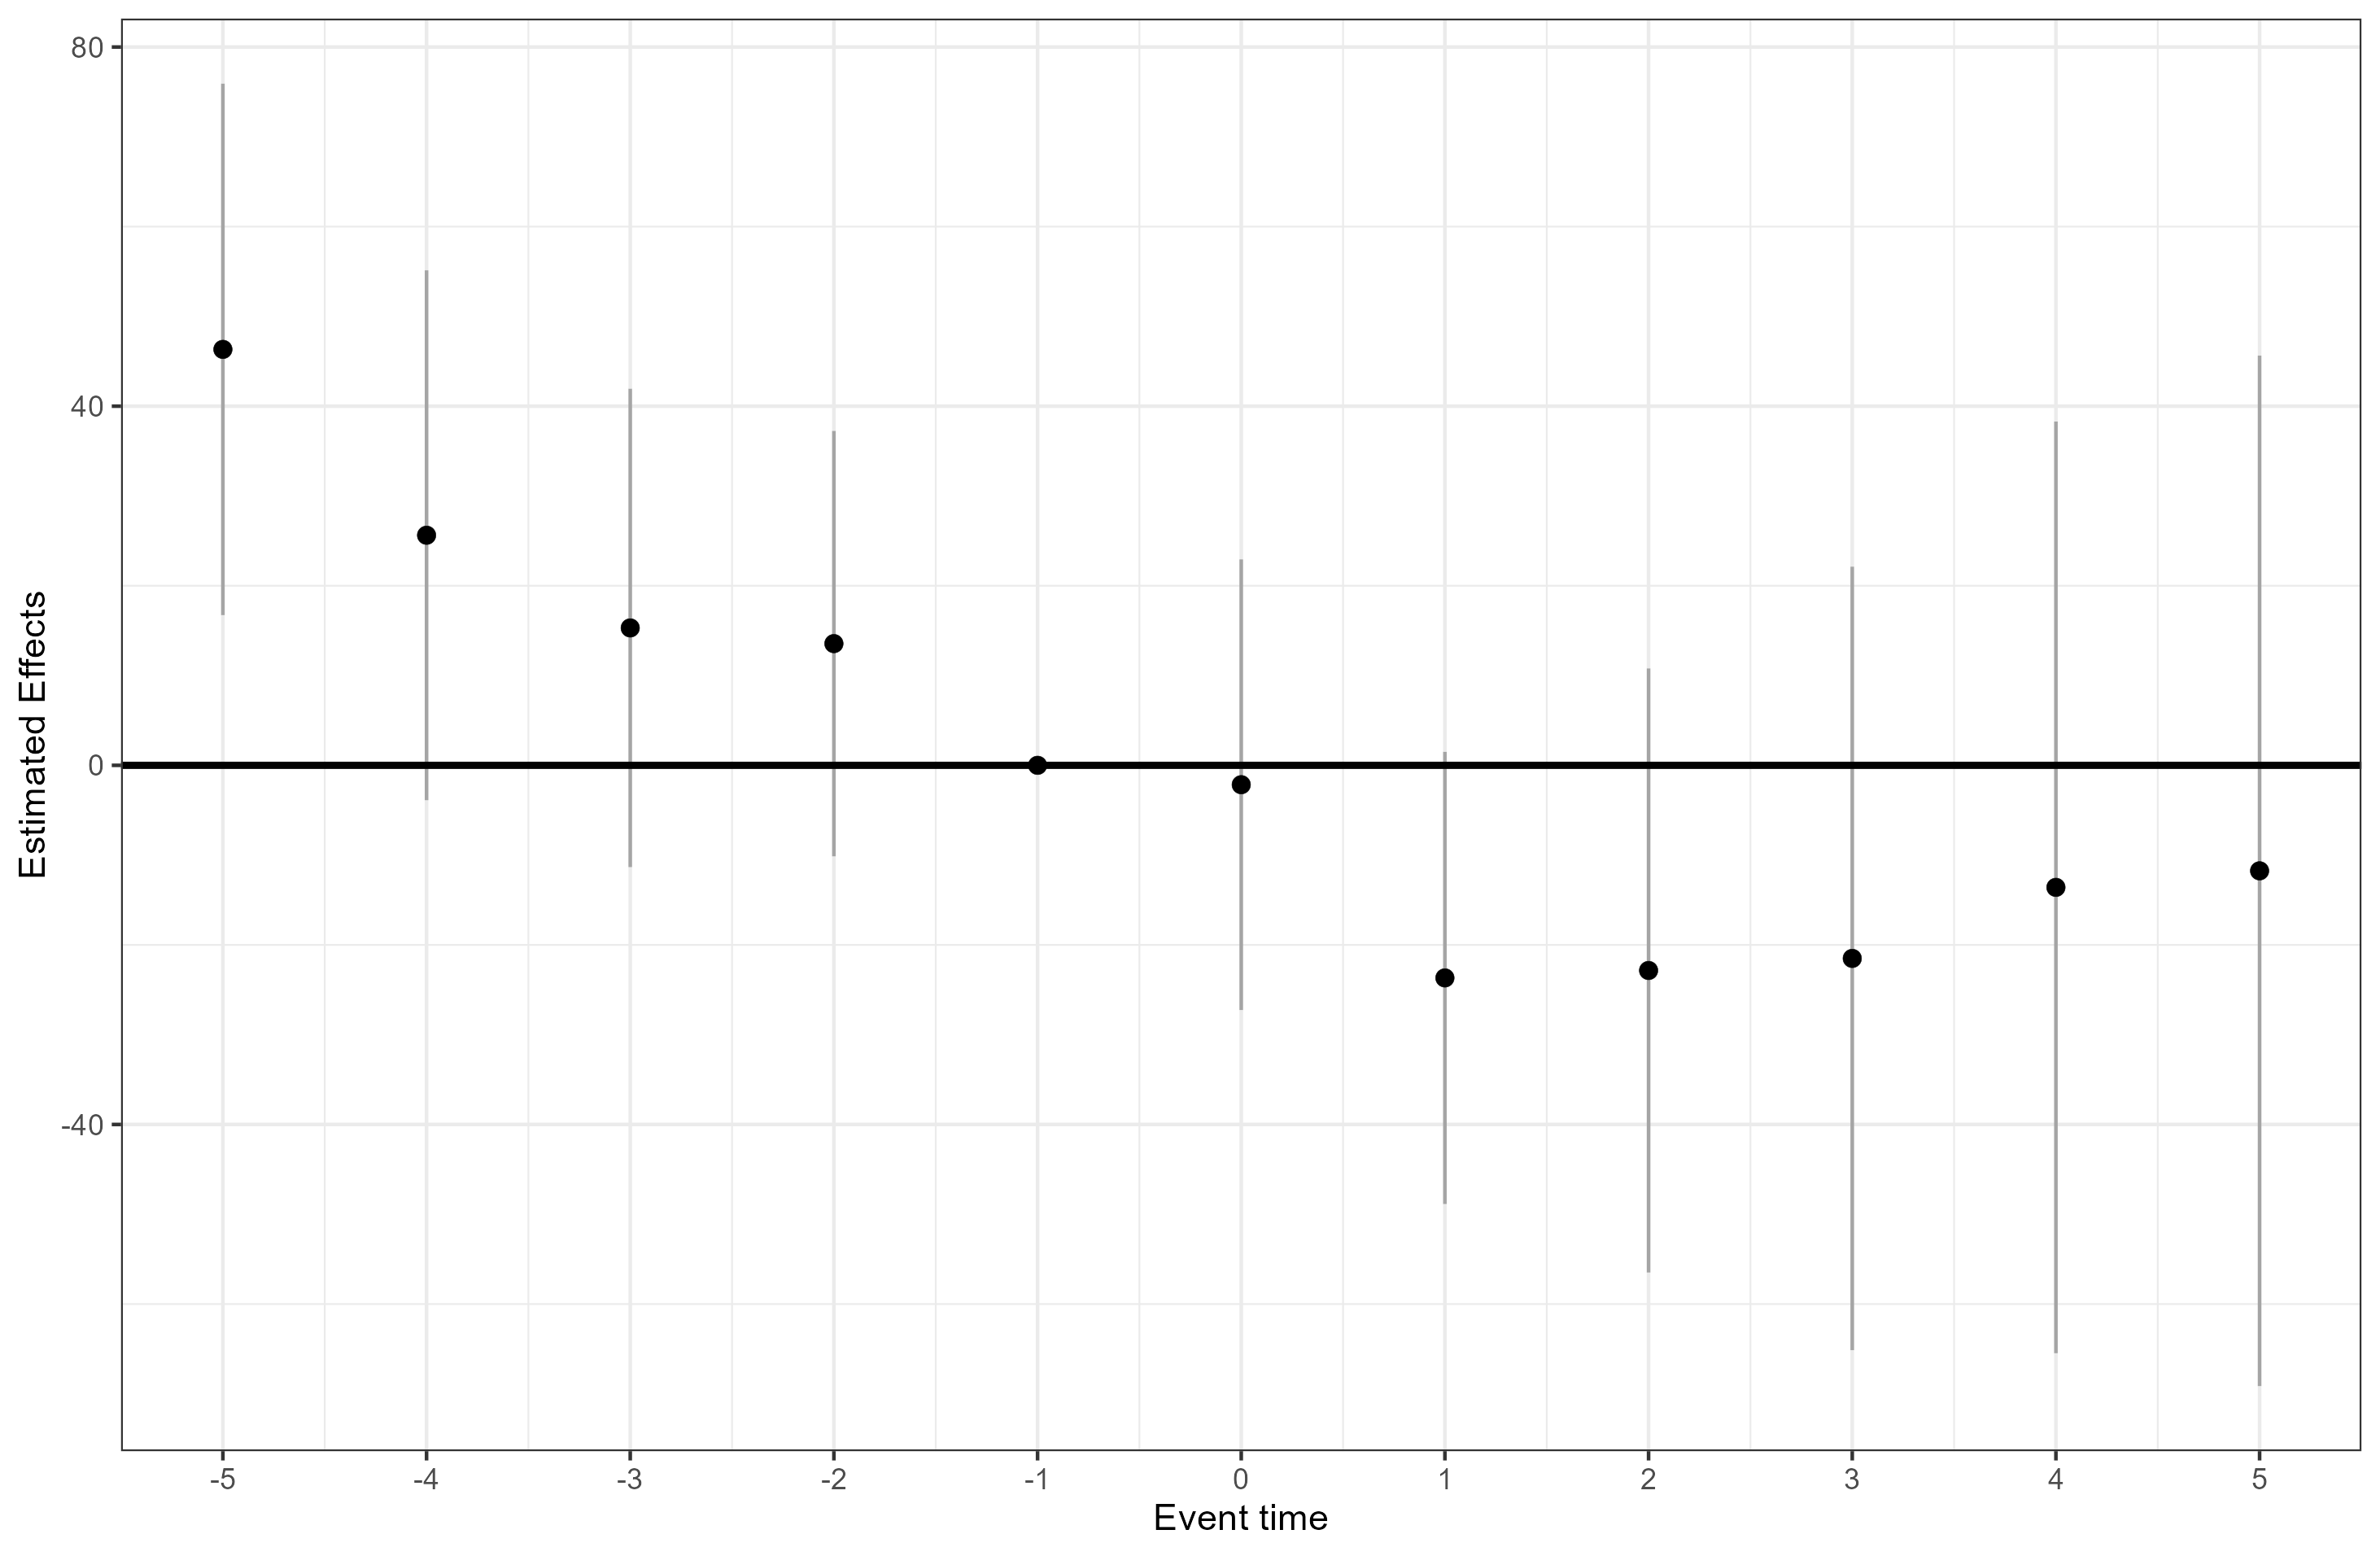
\includegraphics[width=0.48\textwidth]{../results/opvisits-elig-cs.png} &
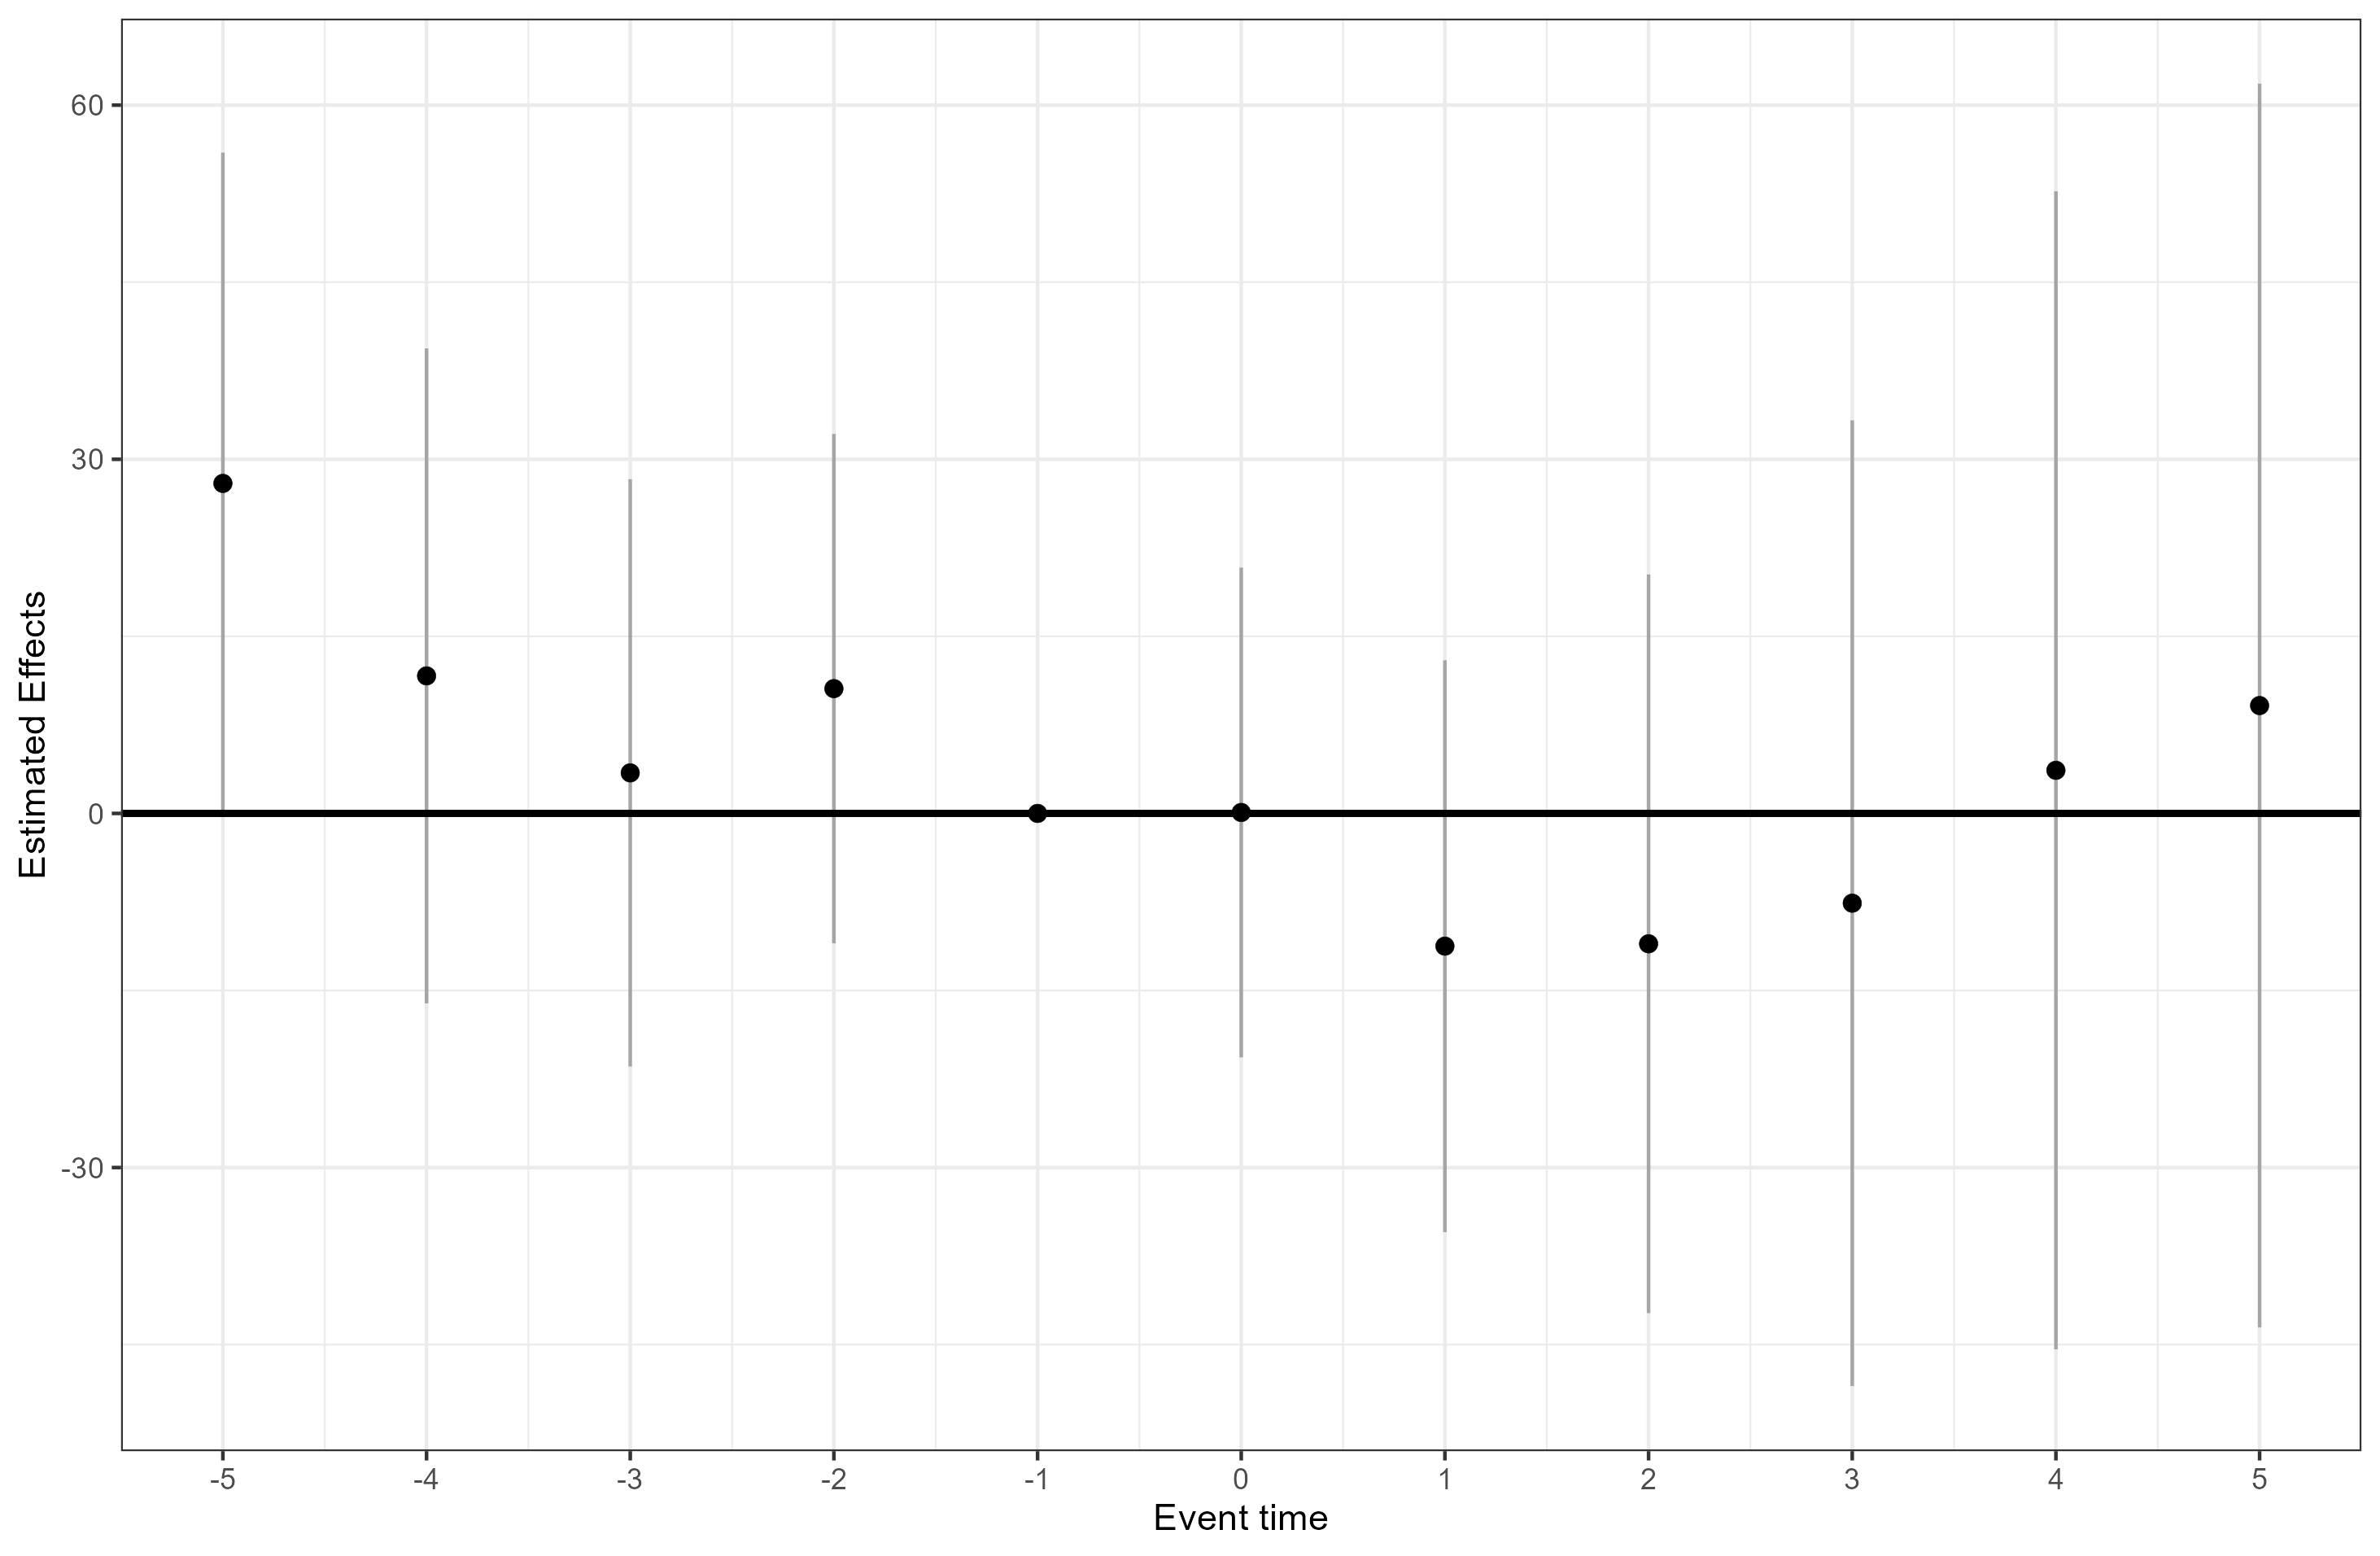
\includegraphics[width=0.48\textwidth]{../results/opvisits-noned-elig-cs.png} \\
\small (a) Outpatient Visits per Bed & \small (b) Non-ED Outpatient Visits per Bed \\[0.5cm]
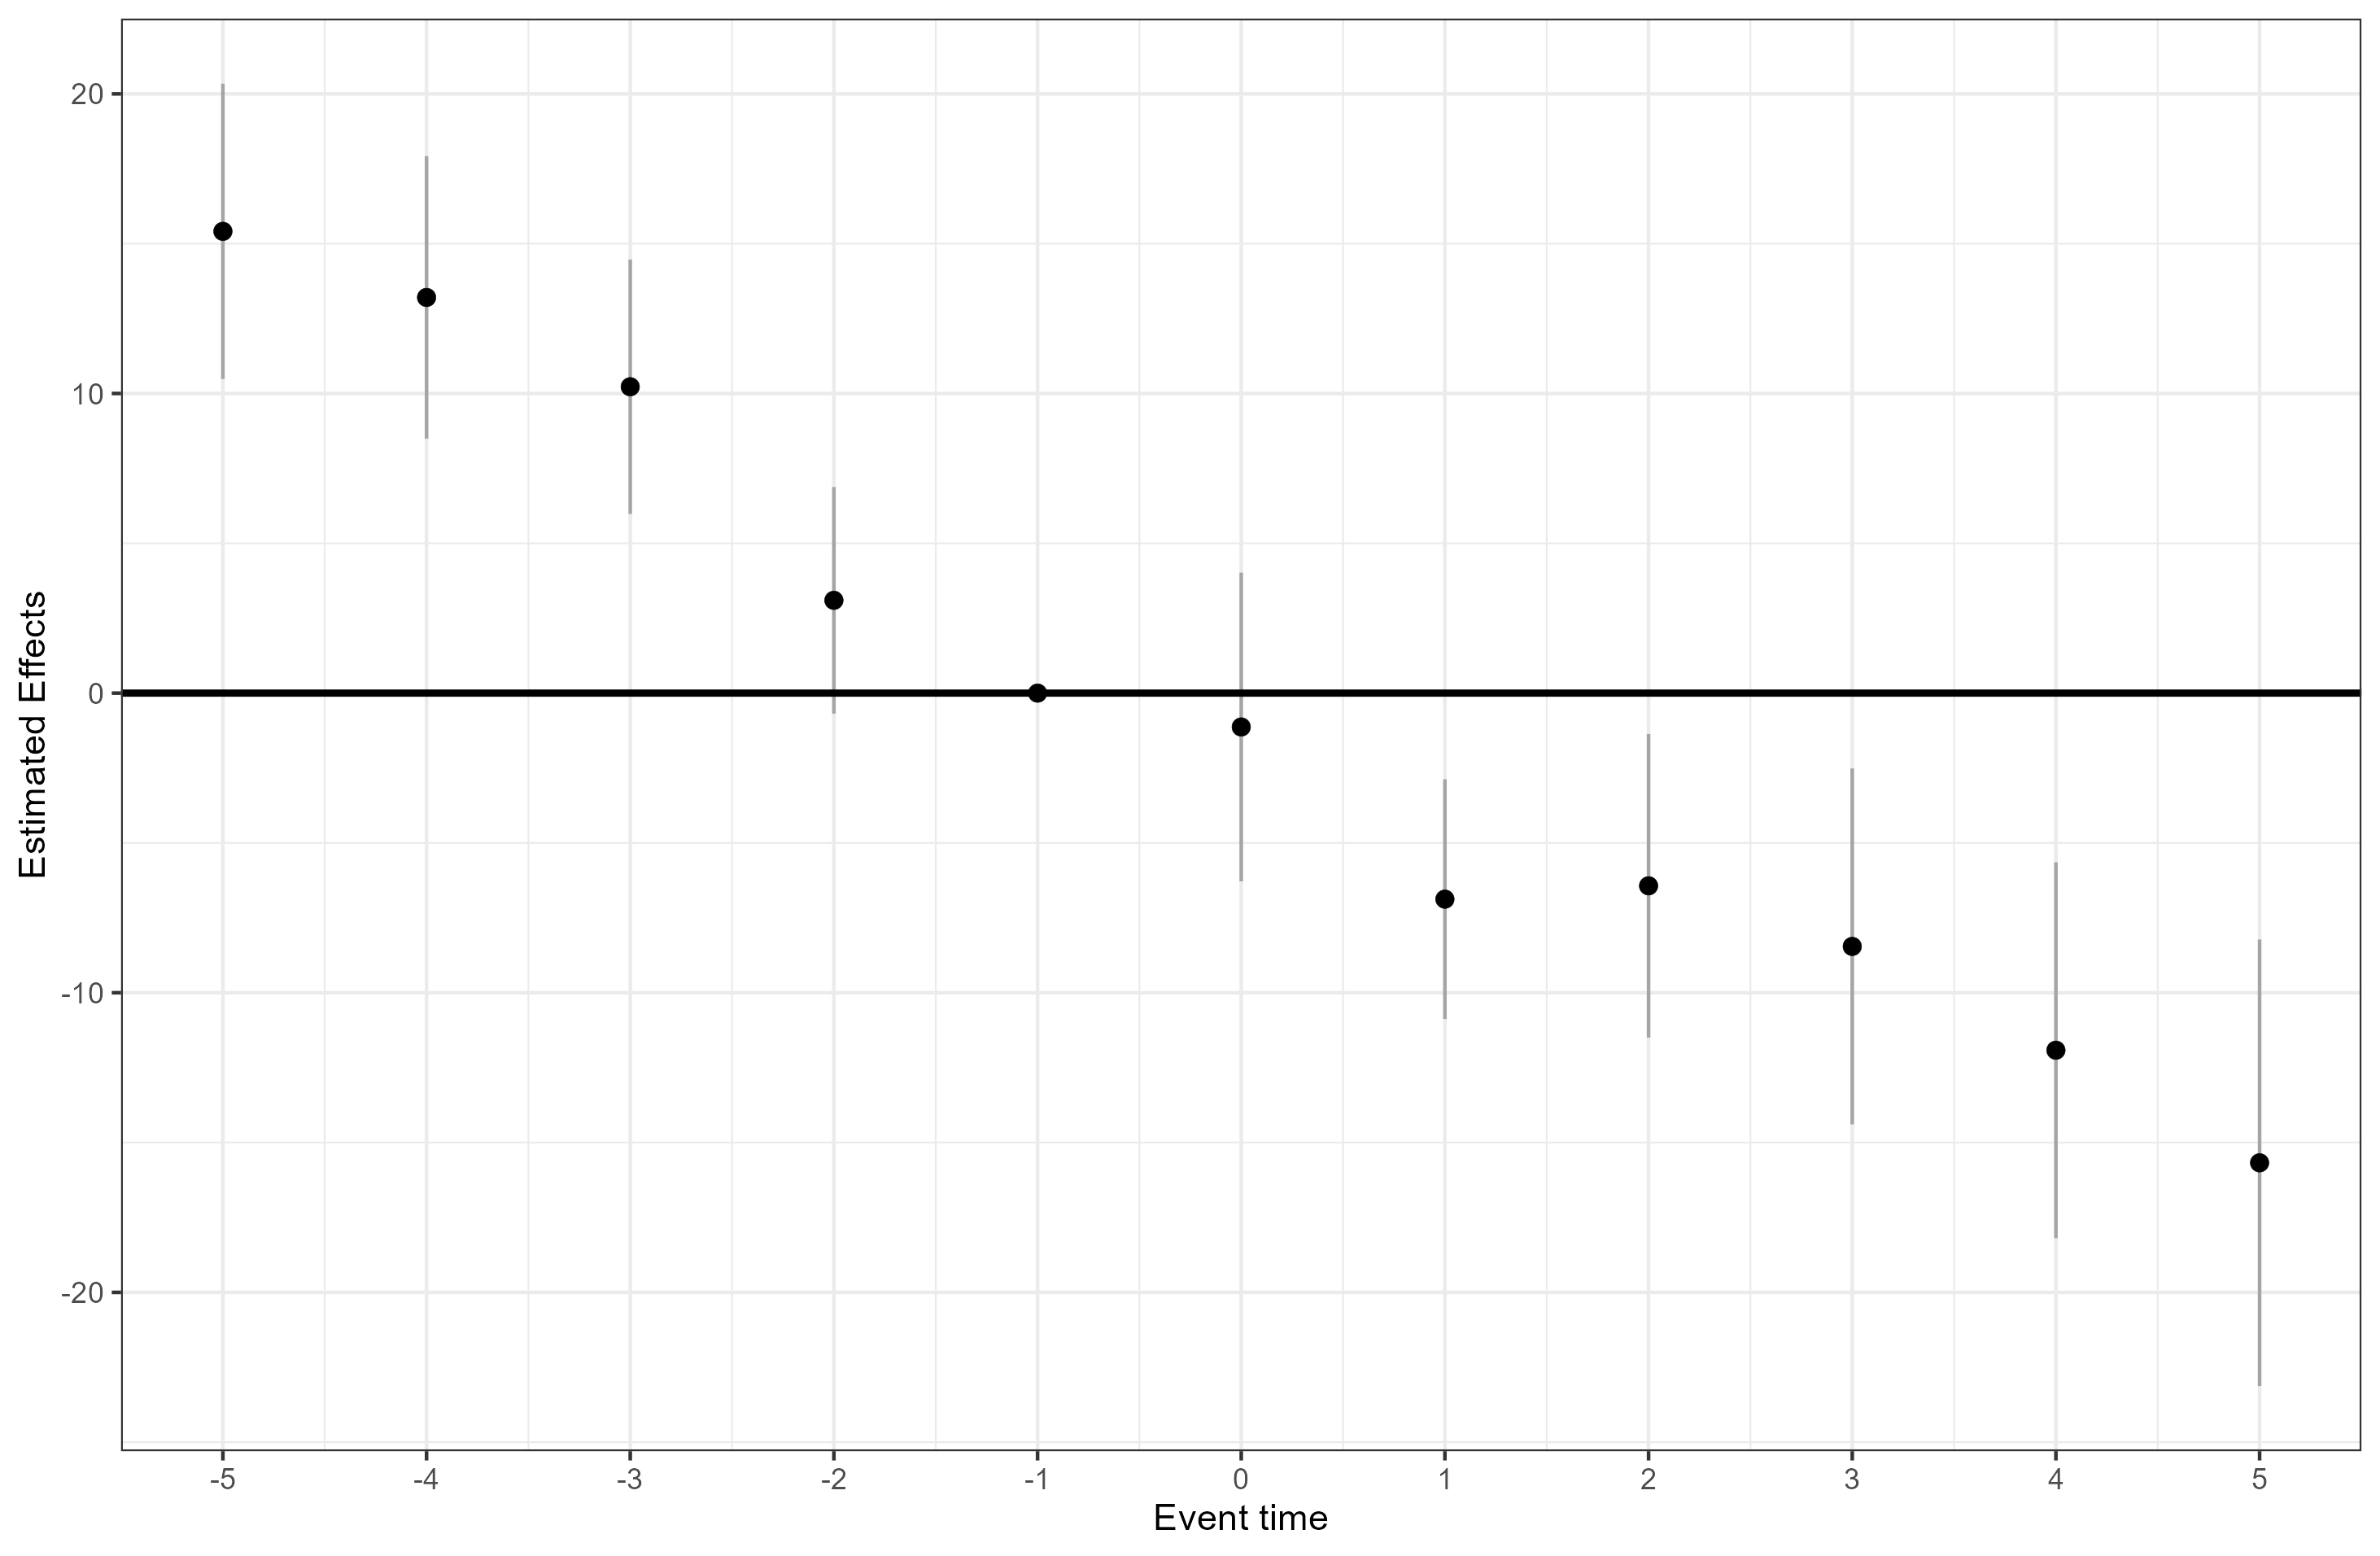
\includegraphics[width=0.48\textwidth]{../results/edvisits-elig-cs.png} &
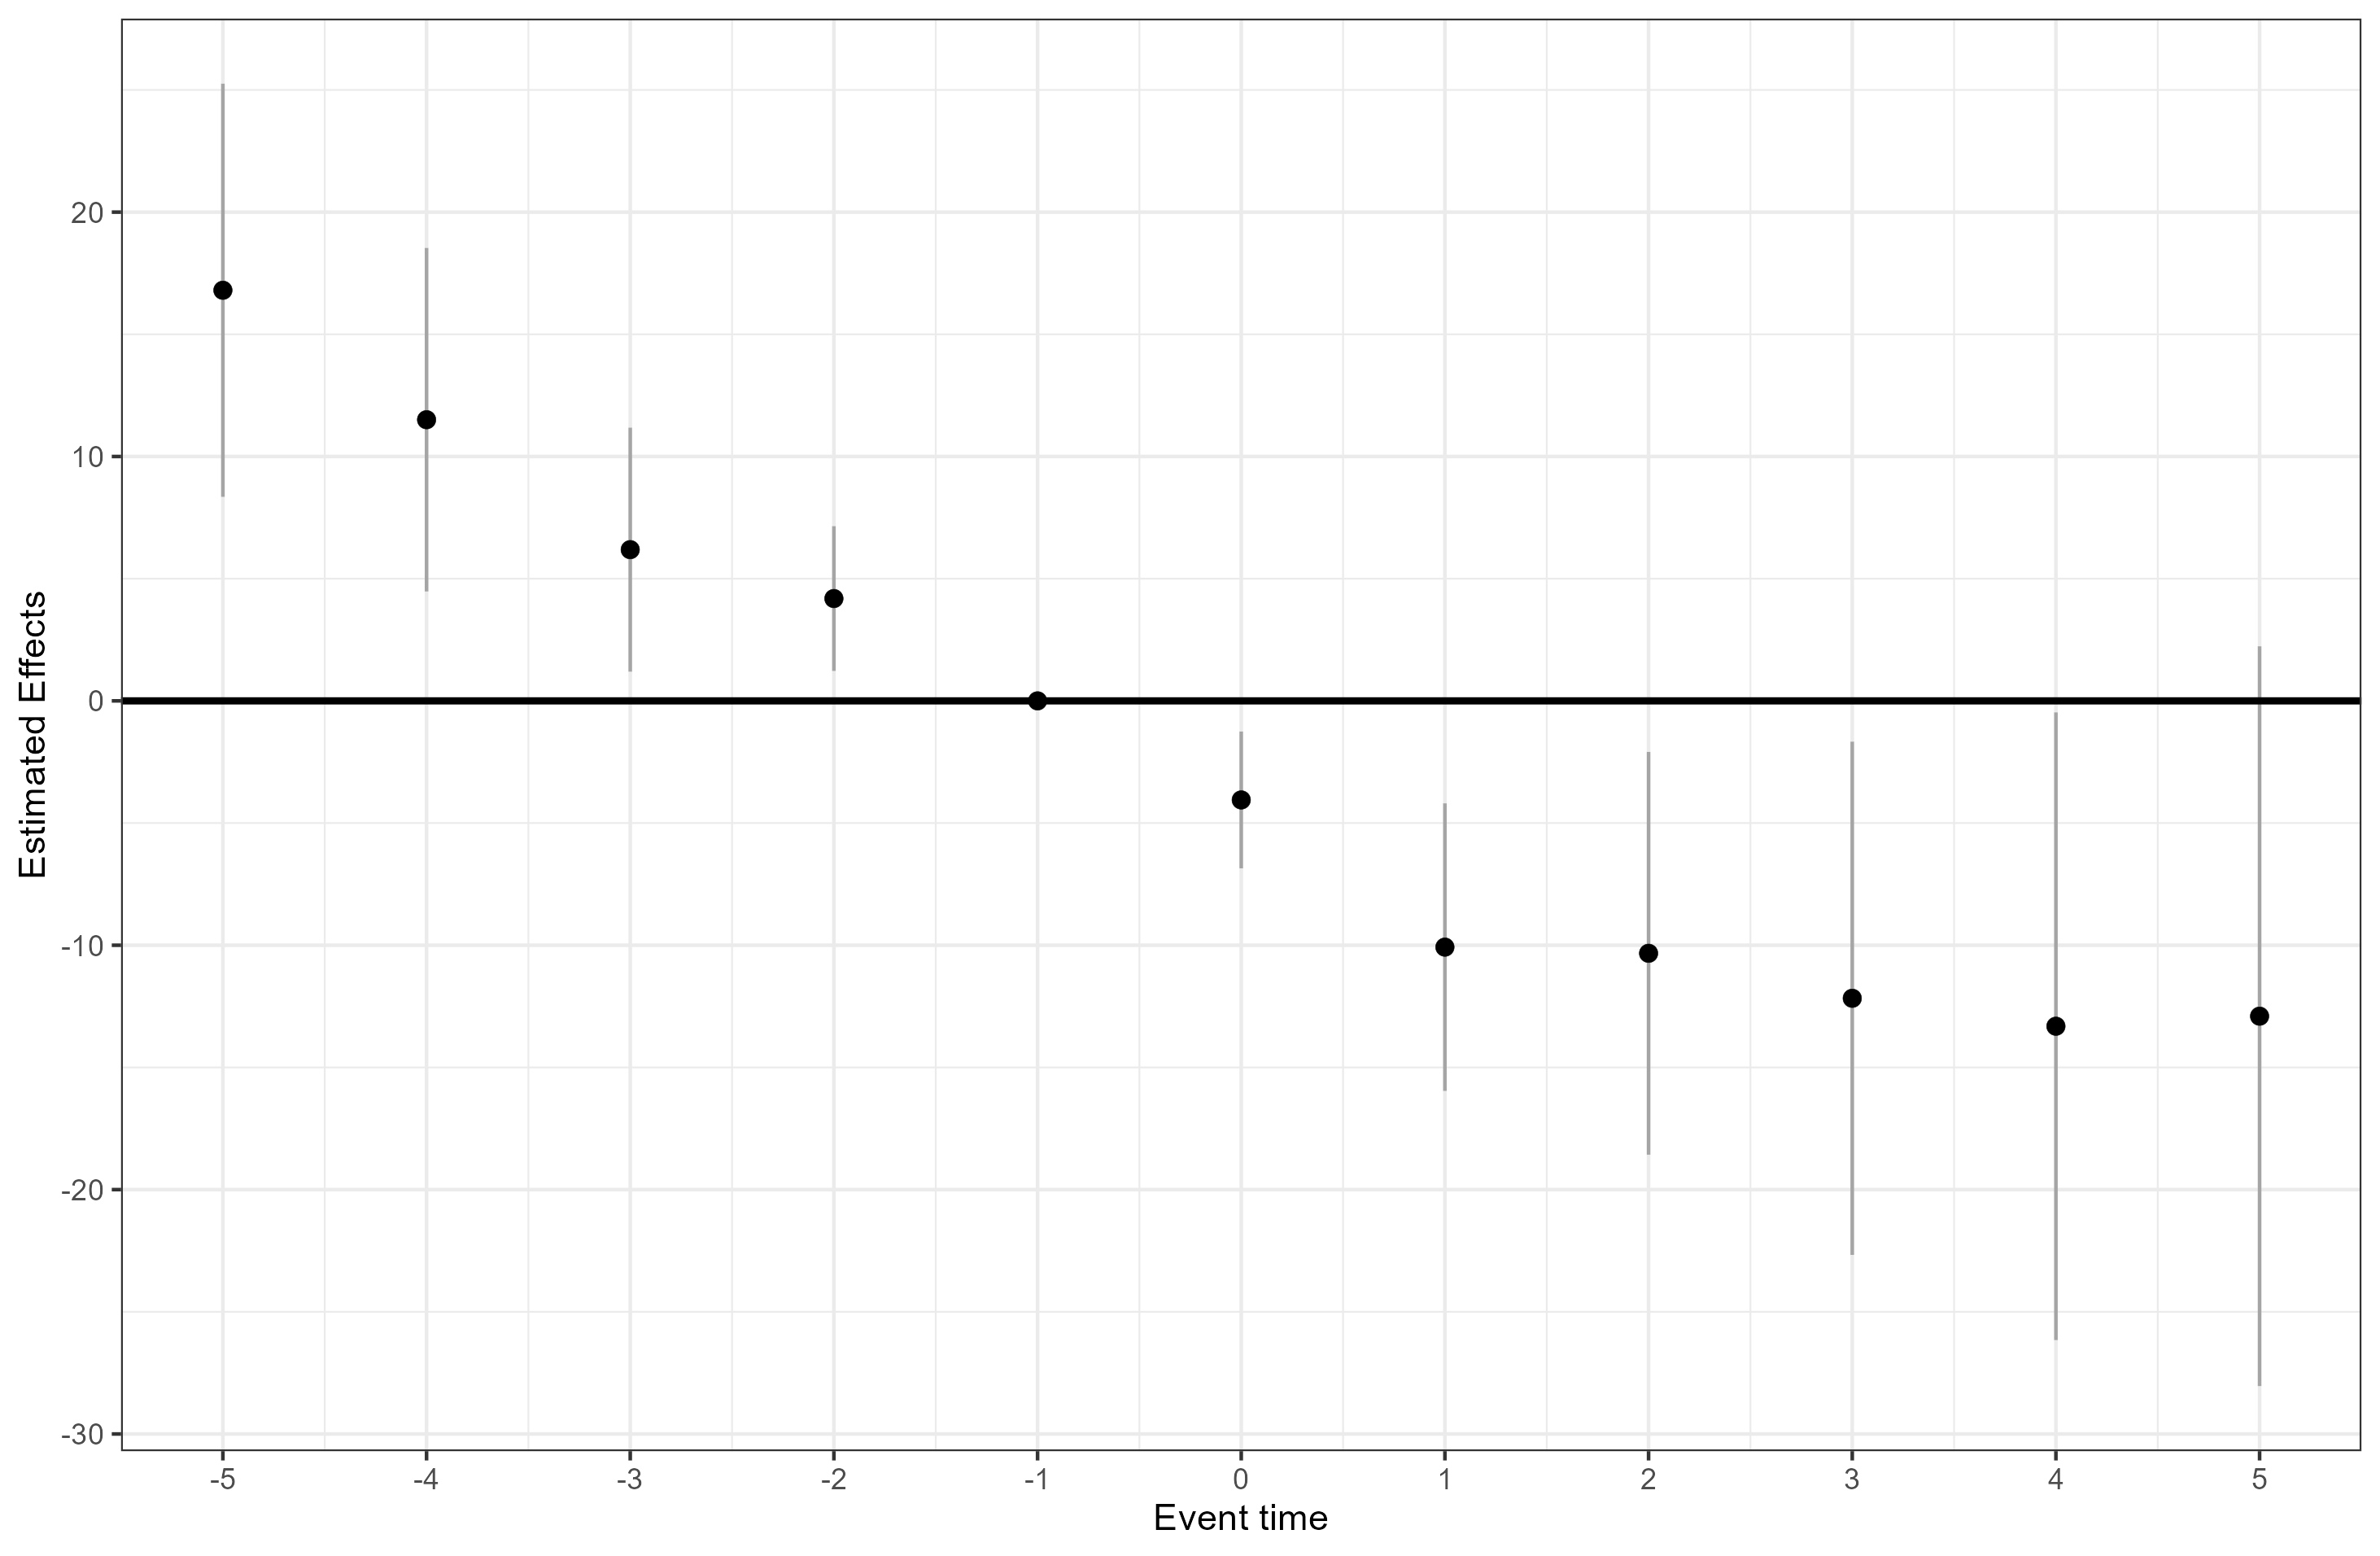
\includegraphics[width=0.48\textwidth]{../results/births-elig-cs.png} \\
\small (c) Emergency Department Visits per Bed & \small (d) Births
\end{tabular}
\end{minipage}
\end{figure}

\clearpage

%%% Permutation Figure

\begin{figure}[!h]
\centering
\begin{minipage}[h]{6in}
\caption[Permutation Inference]{\textbf{Permutation Inference for SDID Estimates}\footnote{Each panel shows the distribution of 500 placebo SDID ATTs obtained by randomly reassigning treatment labels within each cohort's balanced panel. The dashed red line marks the actual SDID estimate. The $p$-value is the two-sided share of placebo ATTs at least as large in absolute value as the observed ATT.}}
\label{fig:permutation}
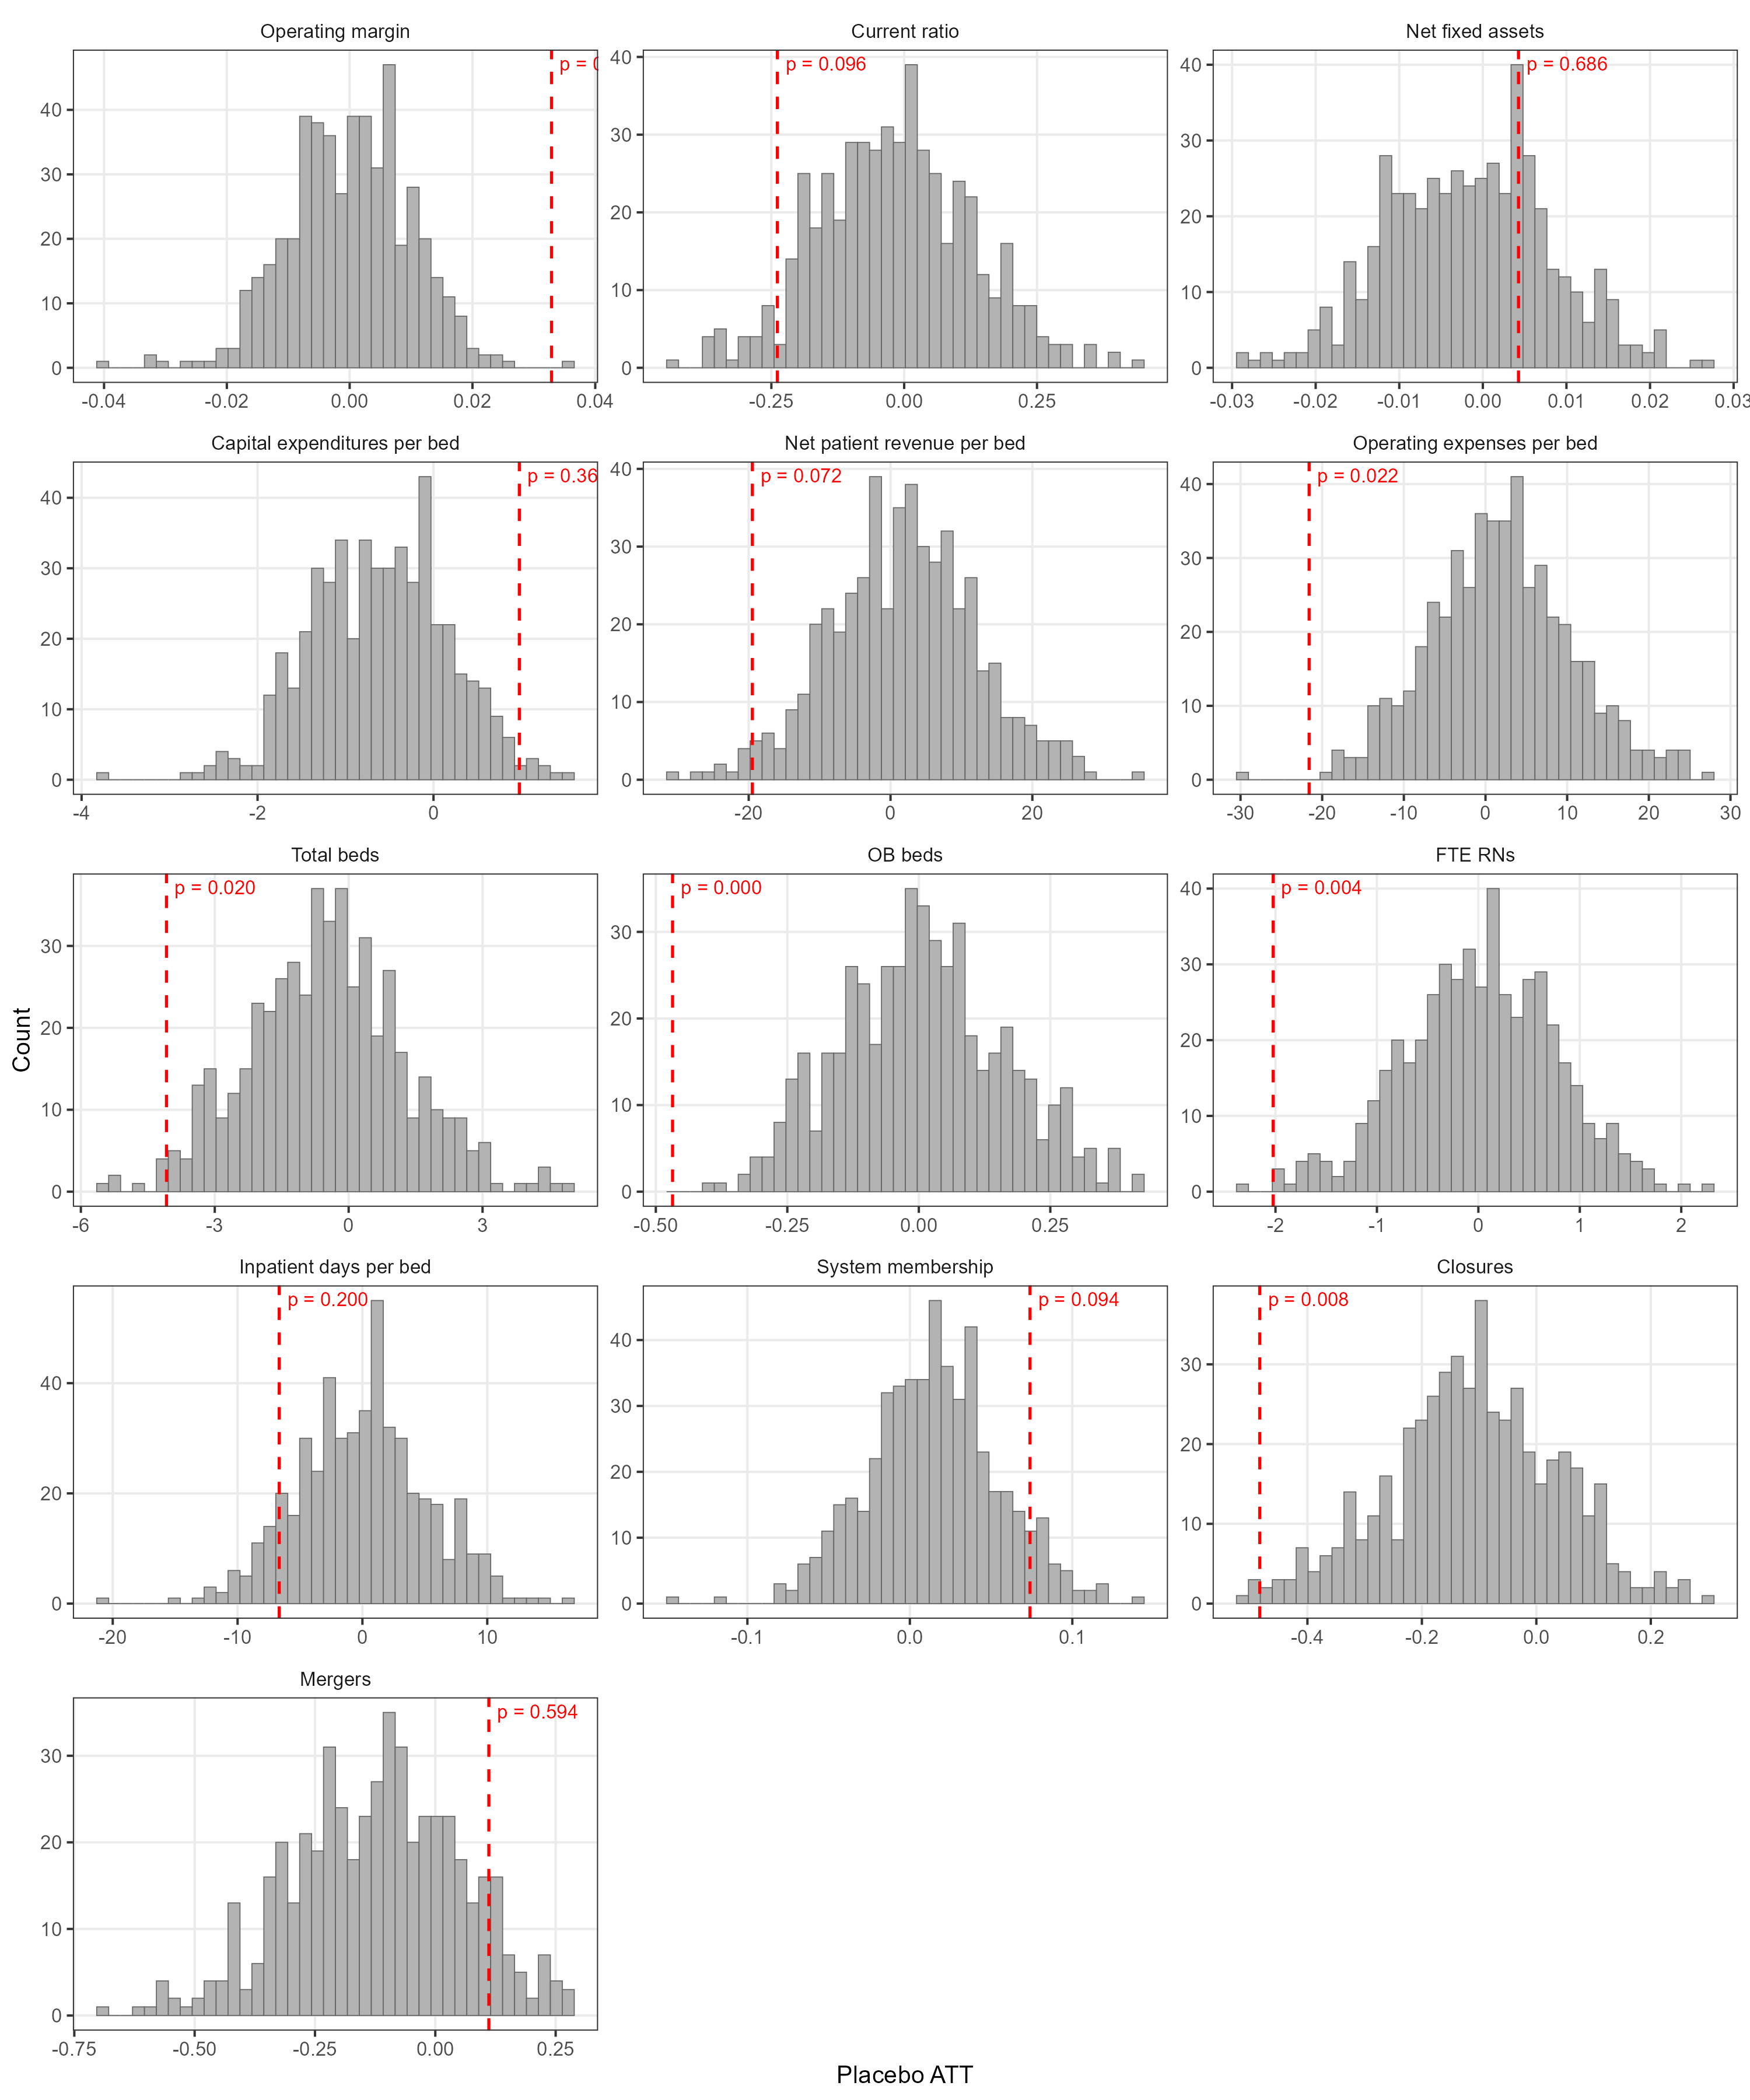
\includegraphics[width=\textwidth]{../results/permutation-sdid.png}
\end{minipage}
\end{figure}

\clearpage
\bibliography{BibTeX_Library}

\end{document}
